
%% Run LaTeX on this file several times to get Table of Contents,
%% cross-references, and citations.

\documentclass[11pt]{book}
\usepackage{Wiley-AuthoringTemplate}
\usepackage[sectionbib,authoryear]{natbib}% for name-date citation comment the below line
%\usepackage[sectionbib,numbers]{natbib}% for numbered citation comment the above line

%%********************************************************************%%
%%       How many levels of section head would you like numbered?     %%
%% 0= no section numbers, 1= section, 2= subsection, 3= subsubsection %%
\setcounter{secnumdepth}{3}
%%********************************************************************%%
%%**********************************************************************%%
%%     How many levels of section head would you like to appear in the  %%
%%				Table of Contents?			%%
%% 0= chapter, 1= section, 2= subsection, 3= subsubsection titles.	%%
\setcounter{tocdepth}{2}
%%**********************************************************************%%

%\includeonly{ch01}
\makeindex
%\includeonly{week3/Tuesday}
\includeonly{week3/Thursday}
\begin{document}
%Hello
\frontmatter
%%%%%%%%%%%%%%%%%%%%%%%%%%%%%%%%%%%%%%%%%%%%%%%%%%%%%%%%%%%%%%%%
%%%Command
%% Title Pages
%% Wiley will provide title and copyright page, but you can make
%% your own titlepages if you'd like anyway
%% Setting up title pages, type in the appropriate names here:

\booktitle{A First Course \\ In \\
Linear Algebra}

\subtitle{MAT2040 Notebook}

\AuAff{Prof. Tom Luo\\ The Chinese University of Hongkong, Shenzhen}
\AuAff{Prof. Ruoyu Sun\\ University of Illinois Urbana-Champaign}
%\AuAff{Michael D. Logothetis\\ University of Patras}

%% \\ will start a new line.
%% You may add \affil{} for affiliation, ie,
%\authors{Robert M. Groves\\
%\affil{Universitat de les Illes Balears}
%Floyd J. Fowler, Jr.\\
%\affil{University of New Mexico}
%}

%% Print Half Title and Title Page:
\halftitlepage
\titlepage

%%%%%%%%%%%%%%%%%%%%%%%%%%%%%%%%%%%%%%%%%%%%%%%%%%%%%%%%%%%%%%%%
%% Copyright Page

%\begin{copyrightpage}{year}
%Title, etc
%\end{copyrightpage}

% Note, you must use \ to start indented lines, ie,
% 
 \begin{copyrightpage}{2004}
 Survey Methodology / Robert M. Groves . . . [et al.].
 \       p. cm.---(Wiley series in survey methodology)
 \    ``Wiley-Interscience."
 \    Includes bibliographical references and index.
 \    ISBN 0-471-48348-6 (pbk.)
 \    1. Surveys---Methodology.  2. Social 
 \  sciences---Research---Statistical methods.  I. Groves, Robert M.  II. %
 Series.\\

 HA31.2.S873 2004
 001.4'33---dc22                                             2004044064
 \end{copyrightpage}

%%%%%%%%%%%%%%%%%%%%%%%%%%%%%%%%%%%%%%%%%%%%%%%%%%%%%%%%%%%%%%%%
%% Only Dedication (optional) 

%\dedication{To my parents}

\tableofcontents

%\listoffigures %optional
%\listoftables  %optional

%% or Contributor Page for edited books
%% before \tableofcontents

%%%%%%%%%%%%%%%%%%%%%%%%%%%%%%%%%%%%%%%%%%%%%%%%%%%%%%%%%%%%%%%%
%  Contributors Page for Edited Book
%%%%%%%%%%%%%%%%%%%%%%%%%%%%%%%%%%%%%%%%%%%%%%%%%%%%%%%%%%%%%%%%

% If your book has chapters written by different authors,
% you'll need a Contributors page.

% Use \begin{contributors}...\end{contributors} and
% then enter each author with the \name{} command, followed
% by the affiliation information.

 \begin{contributors}
 \name{Zhi-quan Luo,} Shenzhen Research Institute of Big Data, Lecturer

 \name{Ruoyu Sun,} Industrial and Enterprise Systems Engineering, Lecturer

 \name{Jie Wang,} The Chinese University of Hongkong, Shenzhen, Typer
 \end{contributors}

%%%%%%%%%%%%%%%%%%%%%%%%%%%%%%%%%%%%%%%%%%%%%%%%%%%%%%%%%%%%%%%%
% Optional Foreword:

\begin{foreword}
\lipsum[1-2]
\end{foreword}

%%%%%%%%%%%%%%%%%%%%%%%%%%%%%%%%%%%%%%%%%%%%%%%%%%%%%%%%%%%%%%%%
% Optional Preface:

\begin{preface}
\lipsum[1-1]
\prefaceauthor{}
\where{place\\
 date}
\end{preface}

% ie,
% \begin{preface}
% This is an example preface.
% \prefaceauthor{R. K. Watts}
% \where{Durham, North Carolina\\
% September, 2004}

%%%%%%%%%%%%%%%%%%%%%%%%%%%%%%%%%%%%%%%%%%%%%%%%%%%%%%%%%%%%%%%%
% Optional Acknowledgments:

\acknowledgments
\lipsum[1-2]
\authorinitials{I. R. S.}  

%%%%%%%%%%%%%%%%%%%%%%%%%%%%%%%%
%% Glossary Type of Environment:

% \begin{glossary}
% \term{<term>}{<description>}
% \end{glossary}

%%%%%%%%%%%%%%%%%%%%%%%%%%%%%%%%
\begin{acronyms}
\acro{ASTA}{Arrivals See Time Averages}
\acro{BHCA}{Busy Hour Call Attempts}
\acro{BR}{Bandwidth Reservation}
\acro{b.u.}{bandwidth unit(s)}
\acro{CAC}{Call / Connection Admission Control}
\acro{CBP}{Call Blocking Probability(-ies)}
\acro{CCS}{Centum Call Seconds}
\acro{CDTM}{Connection Dependent Threshold Model}
\acro{CS}{Complete Sharing}
\acro{DiffServ}{Differentiated Services}
\acro{EMLM}{Erlang Multirate Loss Model}
\acro{erl}{The Erlang unit of traffic-load}
\acro{FIFO}{First in - First out}
\acro{GB}{Global balance}
\acro{GoS}{Grade of Service}
\acro{ICT}{Information and Communication Technology}
\acro{IntServ}{Integrated Services}
\acro{IP}{Internet Protocol}
\acro{ITU-T}{International Telecommunication Unit -- Standardization sector}
\acro{LB}{Local balance}
\acro{LHS}{Left hand side}
\acro{LIFO}{Last in - First out}
\acro{MMPP}{Markov Modulated Poisson Process}
\acro{MPLS}{Multiple Protocol Labeling Switching}
\acro{MRM}{Multi-Retry Model}
\acro{MTM}{Multi-Threshold Model}
\acro{PASTA}{Poisson Arrivals See Time Averages}
\acro{PDF}{Probability Distribution Function}
\acro{pdf}{probability density function}
\acro{PFS}{Product Form Solution}
\acro{QoS}{Quality of Service}
\acro{r.v.}{random variable(s)}
\acro{RED}{random early detection}
\acro{RHS}{Right hand side}
\acro{RLA}{Reduced Load Approximation}
\acro{SIRO}{service in random order}
\acro{SRM}{Single-Retry Model}
\acro{STM}{Single-Threshold Model}
\acro{TCP}{Transport Control Protocol}
\acro{TH}{Threshold(s)}
\acro{UDP}{User Datagram Protocol}
\end{acronyms}
\mainmatter
\setcounter{page}{1}

%\begin{introduction}
%
%The word \textit {traffic} becomes \textit {teletraffic} in telecommunications, as communications becomes telecommunications to indicate technology use, e.g., conversation from some distance through phones or Internet. The term teletraffic covers all kinds of computer communication traffic and telecom traffic.  This book includes teletraffic loss models.
%\end{introduction}

\chapter{Week1}

\section{Tuesday}\index{Tuesday_lecture}

\subsection{Introduction}
\subsubsection{\textit{Why do you learn Linear Algebra?}}
\paragraph{Important: LA + Calculus + Probability}

Every SSE student should learn {\emph{Linear Algebra}}, {\emph{Calculus}}, and {\emph{Probability}} to build strong fundation.

\paragraph{Practical: Computation}

Linear Algebra is more widely used than Calculus since we could use this {\emph{powerful}} tool to do discrete computation. (As we know, we can use calculus to deal with something continuous. But how do we do integration when facing lots of \emph{discrete data}? But linear algebra can help us deal with these data.)

\paragraph{Visualize} 

Conncect between \emph{Geometry} and \emph{Algebra}.

Let's take an easy example:
\begin{example}

Let $v$ and $w$ donate two vectors as below:
\[
\begin{array}{ll}
v= \begin{bmatrix}
1 \\ 2
\end{bmatrix},
&
w = \begin{bmatrix}
3 \\ 4
\end{bmatrix}.
\end{array}
\]

Then we can donate these two vectors in the graph:
\begin{center}
\setlength{\unitlength}{0.5 cm}
\begin{picture}(15,3)\thicklines
\put(0,0){\vector(1,2){1}} \put(0,0){\vector(1,0){2}}
\put(-0.2,1){$v$} \put(1,-0.6){$w$} \put(3.2,2){$v+w$}
\put(1,2){\line(1,0){0.2}} \put(0,0){\vector(3,2){3}}
\put(1.4,2){\line(1,0){0.2}} \put(1.8,2){\line(1,0){0.2}}
\put(2.2,2){\line(1,0){0.2}} \put(2.6,2){\line(1,0){0.2}}
\put(8,1){\vector(1,1){2}} \put(8,1){\vector(2,-1){2}}
\put(10,0){\vector(0,1){3}} \put(8.3,1.9){$v$} \put(8.3,0){$w$}
\put(10.5,1){$v-w$}
\end{picture}
\end{center}

And we can also add two vectors to get $v+w$. Additionally, we can change the coefficients in front of $v$ and $w$ to get $v-w$.

In two dimension space, we can visualize the vector in the coordinate. Then let's watch the \emph{three} dimension space.There are four vectors $u$,$v$,$w$ and $b$. We can also denote it in coordinate.

Here we raise a question: Can we denote vector $b$ as a linear combination with the three vectors $u$, $v$, and $w$? That is to say,
\begin{quotation}
Is there exists coefficients $x_1$, $x_2$, $x_3$ such that 
\[
x_1 \begin{pmatrix}
1 \\ 1 \\ 1
\end{pmatrix}+
x_2 \begin{pmatrix}
1 \\ 2 \\ 3
\end{pmatrix}+
x_3 \begin{pmatrix}
1 \\ 3 \\ 4
\end{pmatrix}=
\begin{pmatrix}
2 \\ 5 \\ 7
\end{pmatrix}?
\]
\end{quotation}

Then we only need to solve the system of equations 
\[\left\{ \begin{gathered}
x_1 + x_2 + x_3 = 2 \\
x_1 + 2x_2 + 3x_3 = 5 \\
x_1 + 3x_2 + 4x_3 = 7
\end{gathered} \right.
\implies \begin{pmatrix}
x_1 \\ x_2 \\ x_3
\end{pmatrix} = \begin{pmatrix}
0 \\ 1 \\ 1
\end{pmatrix}
\]
\end{example}
\paragraph{Abstract: Broad Applications}

Don't worry, broad doesn't mean boring. Instead, it means Linear Algebra can applied to lots of applications.

For example, if we denote a sequence of infinite numbers as a tuple that contains infinite numbers, and we denote this tuple as a vector, then we could build \emph{an infinite banach space.} Moreover, Given a function $f:\mathbb{R} \to \mathbb{R}$, we can describle a set of functions as a tuple, then we could build a \emph{function space}. These abstract knowledge may be not covered in this course. We will learn it in future courses.

\subsubsection{What is Linear Algebra?}
The central problem in math is to \emph{solve equations}. And equations can be seperated into two parts, \emph{nonlinear} and \emph{linear} ones. 

Let's look an example of Nonlinear equations below:
\[ 
\left\{ \begin{gathered}
3x_1x_2 + 5x_1^2 + 6x_2 = 9 \\
x_1x_2^2 + 5x_1 + 7x_2^2 = 10
\end{gathered}
\right.
\]

Well, it is a little bit complicated. We don't find a efficient algorithm to solve these equations. But in algebraic geometry course we will solve some nonlinear equations.

What you need to know about in this course is the linear equations and the methodology to solve it.

\begin{definition}[Linear Equations]
A linear equation in $n$ unknowns is the equation of the form
\[
a_1x_1 + a_2x_2 +\dots + a_nx_n = b,
\]
where $a_1,a_2,\dots,a_n,b$ are real numbers and $x_1,x_2,\dots,x_n$ are variables
\end{definition}

\begin{definition}[Linear System of Equations]
Linear system of $m$ equations in $n$ unknowns is the system of the form

\begin{gather}
a_{11}x_1 + a_{12}x_2 + \dots + a_{1n}x_n = b_1 \notag \\ 
a_{21}x_1 + a_{22}x_2 + \dots + a_{23}x_n = b_2 \notag \\
\dots 	\notag 	\\
a_{m1}x_1 + a_{m2}x_2 + \dots + a_{m3}x_n = b_m , \label{Eq:1.1}
\end{gather}
where $a_{ij}$ and the $b_i$ are all real numbers. We refer to (\ref{Eq:1})as $m \times n$ \emph{linear systems}.
\end{definition}

 
%------------------------------------------------

\subsection{Gaussian Elimination}

Here we mainly focus on $n \times n$ system of equations. 

\begin{example}
Let's recall how to solve a $2 \times 2$ system equatons as below:
\begin{align}
1x_1 + 2x_2 &= 5\label{Eq:1.2}\\
4x_1 + 5x_2 &=14\label{Eq:1.3}.
\end{align}

We can simplify the equation system above into the form (\emph{Augmented matrix}):
\[
\left[
\begin{array}{@{}cc|c@{}}
1 & 2 & 5 \\
4 & 5 & 14
\end{array}
\right]
\]

Secondly, by adding $(-4)\times(\ref{Eq:1.2})$ into (\ref{Eq:1.3}), we obtain:
\begin{align}
{1}x_1 + 2x_2 &=5\label{Eq:1.4}\\
0x_1 + (-3)x_2 &= -6\label{Eq:1.5}
\end{align}

Thirdly, by multiplying $-(1/3)$ of (\ref{Eq:1.5}), we obtain:
\begin{align}
{1}x_1 + 2x_2 &=5 \label{Eq:1.6}\\
1x_2 &= 2\label{Eq:1.7}
\end{align}

Fourthly, by adding $(-2)\times(\ref{Eq:1.7})$ into $(\ref{Eq:1.6})$, we obtain:
\begin{align}
{1}x_1 + 0x_2 &=1 	\\
1x_2 &= 2 
\end{align}

Here we get the solution $(x_1=1, x_2=2)$, and we could write the above process with augmented matrix form:
\[
\left[
\begin{array}{@{}cc|c@{}}
1 & 2 & 5 \\
4 & 5 & 14
\end{array}
\right]
\implies
\left[
\begin{array}{@{}cc|c@{}}
1 & 2 & 5 \\
0& -3 & -6
\end{array}
\right]
\implies
\left[
\begin{array}{@{}cc|c@{}}
1 & 2 & 5 \\
0& 1 & 2
\end{array}
\right]
\implies
\left[
\begin{array}{@{}cc|c@{}}
1 & 0 & 1 \\
0& 1 & 2
\end{array}
\right].
\]
\end{example}

The method shown above is called \emph{Gaussian Elimination}. Here we give a strict definition for Augmented matrix:
\begin{definition}[Augmented matrix]
For the system of equations
\begin{gather}
a_{11}x_1 + a_{12}x_2 + \dots + a_{1n}x_n = b_1 \notag \\ 
a_{21}x_1 + a_{22}x_2 + \dots + a_{2n}x_n = b_2 \notag \\
\dots 	\notag 	\\
a_{m1}x_1 + a_{m2}x_2 + \dots + a_{mn}x_n = b_m , \label{eq:linear system equations_2}
\end{gather}
the corresponding augmented matrix is given by 
\[
\left[
\begin{array}{@{}cccc|c@{}}
a_{11} & a_{12} & \dots & a_{1n} &  b_1 \\
a_{21} & a_{22} & \dots & a_{2n} &  b_2 \\
\vdots    & \vdots    & \ddots & \vdots    & \vdots \\
a_{m1} & a_{m2} & \cdots & a_{mn} &   b_n
\end{array}
\right].
\]
\end{definition}

We give the definition for a new term \emph{pivot}:
\begin{definition}[pivot]
Returning to the example, we find after third step the matrix is given by 
\[
\left[
\begin{array}{@{}cc|c@{}}
1 & 2 & 5 \\
0 & 1 & 2
\end{array}
\right].
\]

We find that the second row will be used to eliminate the element in the second column of the first row. Here we refer to the second row as the \emph{pivot
row}. The first nonzero entry in the pivotal row is called the \emph{pivot}. For the example case, the element in the second column of the second row is the pivot.
\end{definition}

\subsubsection{How to visualize the system of equation?}
Here we try to visualize the system of equation $
\left \{	\begin{gathered}
1x_1 + 2x_2 =5	\\
4x_1 + 5x_2 = 14 
\end{gathered}	\right.$:

\paragraph{Row Picture} Focusing on the row of the system of equation, we can denote each equation as a line on the coordinate axis. And the solution denote the coordinate.

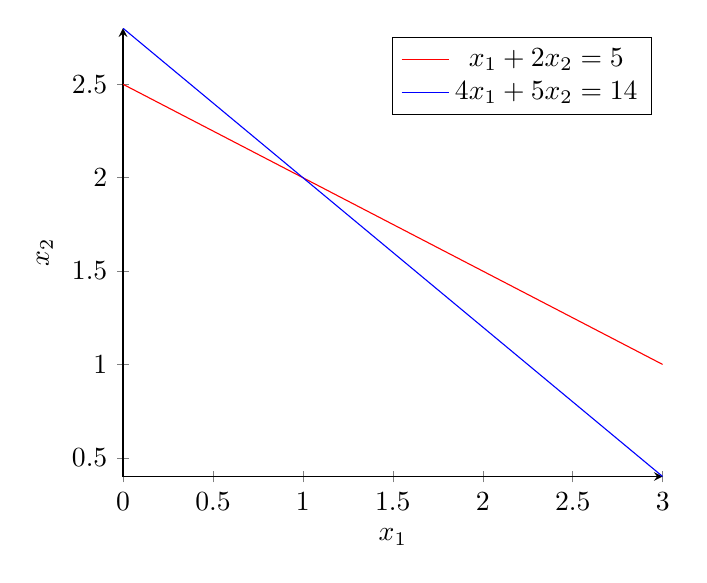
\begin{tikzpicture}
\begin{axis}[
    axis lines = left,
    xlabel = $x_1$,
    ylabel = {$x_2$},
]
%Below the red parabola is defined
\addplot [
    domain=0:3, 
    samples=100, 
    color=red,
]
{2.5-0.5*x};
\addlegendentry{$x_1+2x_2=5$}
%Here the blue parabloa is defined
\addplot [
    domain=0:3, 
    samples=100, 
    color=blue,
    ]
    {-0.8*x+2.8};
\addlegendentry{$4x_1+5x_2=14$}
\end{axis}
\end{tikzpicture}
\paragraph{Column Picture} Focusing on the column of the system of equation, we can denote 
$\begin{bmatrix}
1\\4
\end{bmatrix}$ and $\begin{bmatrix}
2\\5
\end{bmatrix}
$ as vectors in coordinate axis. {Could the linear combinations of these two vectors form the vector}
$\begin{bmatrix}
5\\14
\end{bmatrix}$?  If we denote $x_1$ and $x_2$ as coefficients, it suffices to solve the equation 
$
x_1\begin{bmatrix}
1\\4
\end{bmatrix} + x_2\begin{bmatrix}
2\\5
\end{bmatrix} = \begin{bmatrix}
5\\14
\end{bmatrix}$.

\subsubsection{The solutions of the Linear System of Equations}
The solution to linear system equation could only be \emph{unique}, \emph{infinite}, or \emph{empty}. Let's talk about it case by case in graphic way:
\paragraph{Case 1: unique solution} If two lines intersect at one point, then there is unique solution.
\begin{center}
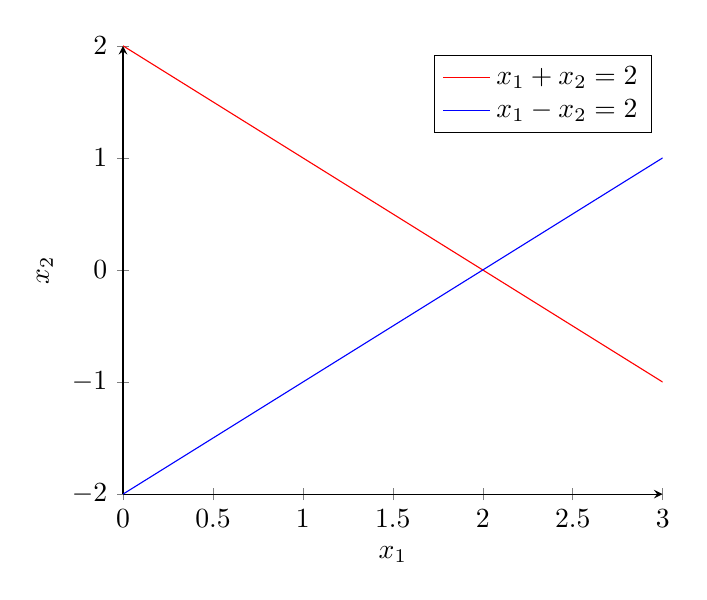
\begin{tikzpicture}
\begin{axis}[
    axis lines = left,
    xlabel = $x_1$,
    ylabel = {$x_2$},
]
%Below the red parabola is defined
\addplot [
    domain=0:3, 
    samples=100, 
    color=red,
]
{2-x};
\addlegendentry{$x_1+x_2=2$}
%Here the blue parabloa is defined
\addplot [
    domain=0:3, 
    samples=100, 
    color=blue,
    ]
    {x-2};
\addlegendentry{$x_1-x_2=2$}
\end{axis}
\end{tikzpicture}
\end{center}
\paragraph{Case2: no solution} If two lines are parallel, then there is no solution.
\begin{center}
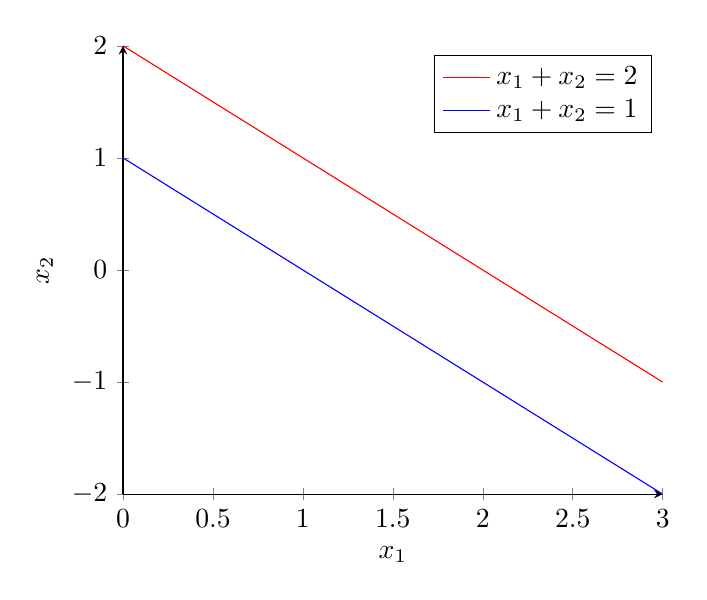
\begin{tikzpicture}
\begin{axis}[
    axis lines = left,
    xlabel = $x_1$,
    ylabel = {$x_2$},
]
%Below the red parabola is defined
\addplot [
    domain=0:3, 
    samples=100, 
    color=red,
]
{2-x};
\addlegendentry{$x_1+x_2=2$}
%Here the blue parabloa is defined
\addplot [
    domain=0:3, 
    samples=100, 
    color=blue,
    ]
    {1-x};
\addlegendentry{$x_1+x_2=1$}
\end{axis}
\end{tikzpicture}
\end{center}
\paragraph{Case 3: infinite number of solutions} If both equations represent the same line, then there are infinite number of solutions.
\begin{center}
\begin{tikzpicture}
\begin{axis}[
    axis lines = left,
    xlabel = $x_1$,
    ylabel = {$x_2$},
]
%Below the red parabola is defined
\addplot [
    domain=0:3, 
    samples=100, 
    color=red,
]
{2-x};
\addlegendentry{$x_1+x_2=2$}
%Here the blue parabloa is defined
\addplot [
    domain=0:3, 
    samples=100, 
    color=blue,
    ]
    {2-x};
\addlegendentry{$-x_1-x_2=-2$}
 
\end{axis}
\end{tikzpicture}
\end{center}
\subsubsection{How to solve $3 \times 3$ Systems?}

\begin{example} \qquad
\\
Let's recall how to solve a $3 \times 3$ system equations as below:

\[
\left \{	\begin{gathered}
2x_1 + x_2 +x_3=5 	\\
4x_1 + (-6)x_2 = -2 \\
-2x_2+7x_2+2x_3 = 9
\end{gathered}	\right.
\]
We can simplify the equation system above into the \emph{Augmented matrix} form:
\[
\left \{	\begin{gathered}
2x_1 + x_2 +x_3=5 	\\
4x_1 + (-6)x_2 = -2 \\
-2x_2+7x_2+2x_3 = 9
\end{gathered}	\right.
\qquad \implies \qquad
\left[
\begin{array}{@{}ccc|c@{}}
2 & 1 & 1 & 5\\
4 & -6 & 0 & -2\\
-2 & 7 & 2 & 9
\end{array}
\right]
\]
%
\[
\xLongrightarrow[\text{Add row 1 to row 3}]{\text{Add $(-2)\times$ row 1 to row 2}}{\quad\quad}
\left[
\begin{array}{@{}ccc|c@{}}
2 & 1 & 1 & 5\\
0 & -8 & -2 & -12\\
0 & 8 & 3 & 14
\end{array}
\right]
\]
\[\xLongrightarrow{\text{Add row 2 to row 3}}{\quad\quad}
\left[
\begin{array}{@{}ccc|c@{}}
2 & 1 & 1 & 5\\
0 & -8 & -2 & -12\\
0 & 0 & 1 & 2
\end{array}
\right]\]
This augmented matrix is the \emph{strictly triangular system}, and it's trial to get the final solution:
\[\implies
\begin{pmatrix}
x_1\\x_2\\x_3
\end{pmatrix}=
\begin{pmatrix}
1\\1\\2
\end{pmatrix}\]
\end{example}

Here we give the definition for strictly triangular system:
\begin{definition}[strictly triangular system]
For the augmented matrix
\[
\left[
\begin{array}{@{}cccc|c@{}}
a_{11} & a_{12} & \dots & a_{1n} &  b_1 \\
a_{21} & a_{22} & \dots & a_{2n} &  b_2 \\
\vdots    & \vdots    & \ddots & \vdots    & \vdots \\
a_{m1} & a_{m2} & \cdots & a_{mn} &   b_n
\end{array}
\right],
\]
if in the $k$th row, the first $(k-1)$th column entries are \textit{all zero} and the $k$th column entries is nonzero, we say the augmented matrix(or corresponding system equation) is of \emph{strictly triangular form}. This kind of matrix(or corresponding system equation) is called \emph{strictly triangular system}.
$(k = 1, . . . , m).$
\end{definition}

\subsubsection{How to solve $n \times n$ System?}
We try to reduce an $n \times n$ System to strictly triangular form. Let's take a special example:
\begin{example}
Given an $n \times n$ System of the form:
\begin{equation}\left[
\begin{array}{@{}cccc|c@{}}
a_{11} & a_{12} & \dots & a_{1n} &  b_1 \\
a_{21} & a_{22} & \dots & a_{2n} &  b_2 \\
\vdots    & \vdots    & \ddots & \vdots    & \vdots \\
a_{n1} & a_{n2} & \cdots & a_{nn} &   b_n
\end{array}\right]\label{eq:n*n_matrix}\end{equation}
Assuming the \emph{diagonal entries} are always \textit{nonzero} during our operation. 
Add row 1 that multiplied by a constant to other $n-1$ row to ensure the first entry of other $n-1$ rows are all \textit{zero}:
\begin{equation}
\implies 
\left[
\begin{array}{@{}cccc|c@{}}
a_{11} & a_{12} & \dots & a_{1n} &  b_1 \\
0 & \x & \dots & \x &  \x \\
\vdots    & \vdots    & \ddots & \vdots    & \vdots \\
0 & \x & \cdots & \x &   \x
\end{array}
\right] \label{eq:n*n_matrix_version1}\end{equation}


Then we proceed this way $n-1$times to obtain:
\begin{equation}
  \left[
    \begin{array}{@{}ccccc|c@{}}
    \x    & \x       & \x    & \x    & \x & \x\\ \cline{1-1}
    \bord & \x       & \x    & \x    & \x & \x\\ \cline{2-2}
          & \bord    & \x    & \x    & \x & \vdots \\ \cline{3-3}
          & \bigzero & \bord & \x    & \x & \vdots \\ \cline{4-4}
          &          &       & \bord & \x & \x \\ \cline{5-5}
  \end{array}\right]\label{eq:n*n_matrix_version2}
\end{equation}

This matrix is the \emph{Row-echelon form}.
And we do the back substitution again to obtain:
\begin{equation}
  \left[
    \begin{array}{@{}ccccc|c@{}}
    \x    &        &     &     &  & \x\\ \cline{1-1}
    \bord & \x       &     &     & \bigzero & \x\\ \cline{2-2}
          & \bord    & \x    &     &  & \vdots \\ \cline{3-3}
          & \bigzero & \bord & \x    &  & \vdots \\ \cline{4-4}
          &          &       & \bord & \x & \x \\ \cline{5-5}
  \end{array}\right]\label{eq:n*n_matrix_version3}
\end{equation}
This matrix is the \emph{Reduced Row-Echelon Form}.
Finally by multiplying every row by a nonzero constant to ensure its \emph{diagnoal entries} are all $1$:
\begin{equation}
  \left[
    \begin{array}{@{}ccccc|c@{}}
    1    &        &     &     &  & \x\\ \cline{1-1}
    \bord & 1       &     &     & \bigzero & \x\\ \cline{2-2}
          & \bord    & \ddots    &     &  & \vdots \\ \cline{3-3}
          & \bigzero & \bord & 1    &  & \vdots \\ \cline{4-4}
          &          &       & \bord & 1 & \x \\ \cline{5-5}
  \end{array}\right]\label{eq:n*n_matrix_version4}
\end{equation}
\end{example}

Then let's analysis the complexity of solving such a $n\times n$ system.
\subsection{Complexity Analysis}
\subsubsection{Step1: Reduction from matrix (\ref{eq:n*n_matrix}) to matrix (\ref{eq:n*n_matrix_version1})}
\begin{proposition}
The time complexity for Augmented matrix reduction using back-substitution algorithm is $\mathcal{O}(n^3)$.
\end{proposition}

\begin{proof}
The estimation for the time complexity requires us to estimate how many steps of \emph{multiplication} we need. (The time for addition is so small that can be ignored).
\begin{itemize}
\item
Reducing matrix (\ref{eq:n*n_matrix}) to matrix (\ref{eq:n*n_matrix_version1}) we need to do $n(n-1)$times multiplications.

This is because for each row (except first row) we have known the first entry is zero, while the remaining $(n-1)$ entries in each row should be computed by multiplying first row's entries and then add it to the row.
\item
Then it suffices to deal with the inner $(n-1)\times (n-1)$ matrix, which requires the $(n-1)\times (n-2)$ times multiplication.
\item
The back substitution for matrix (\ref{eq:n*n_matrix}) requires $n$ times reduction.
\end{itemize}
Hence the total multiplication times for back substitution for matrix (\ref{eq:n*n_matrix}) is
\begin{equation*}
\begin{split}
\sum_{i=1}^n i(i-1)
	&= \sum_{i=1}^n (i^2-i)  \\
 		&=\sum_{i=1}^n i^2 - \sum_{i=1}^n i \\
		&=\frac{n(n+1)(2n+1)}{6} - \frac{n(n+1)}{2} \\
		&=\frac{n^3-2n}{3} \sim \frac{n^3}{3} =O(n^3)
\end{split}
\end{equation*}
\end{proof}
But we can always develop more advanced algorithm that have smaller time complexity.

\subsubsection{Step2: Reduction from triangular system to diagonal system}

In order to reducing matrix (\ref{eq:n*n_matrix_version2}) to matrix (\ref{eq:n*n_matrix_version3}) we need to do back-substitution again. The matrix (\ref{eq:n*n_matrix_version3}) is diagonal system. Obviously, for this process the total multiplication times is given by
\[
1+2+\cdots+n-1 = \frac{n(n-1)}{2} \sim O(n^2)
\]
\subsubsection{Step3: Get final solution}

In the final step, we want to reduce matrix (\ref{eq:n*n_matrix_version3}) to matrix (\ref{eq:n*n_matrix_version4}), the only thing we need to do is to do one multiplication for each row to let the diagonal entries be $1$. Hence the total multiplication times for this process is given by
\[
\underbrace{1+1+\dots+1}_{\text{totally $n$ terms}} = O(n)
\]
\subsection{Brief Summary}
The reduction of $n\times n$ matrix requires three kinds of Row operations:
\begin{itemize}
\item \emph{Addition and Multiplication}.

Add to a row by a constant multiple of another row.

\item \emph{Multiplication}

Multiply a row by a nonzero constant.
\item \emph{Interchange}

Interchange two rows
\end{itemize}


\begin{enumerate}
\item
agds
\end{enumerate}•
\section{Thursday}\index{Thursday_lecture}

\subsection{Row-Echelon Form}
\subsubsection{Gaussian Elimination does't always work}

Let's discuss an example to introduce the concept for row-echelon form.
\begin{example}
We apply Gaussian Elimination to try to transfrom a  Augmented matrix:
\begin{itemize}
\item
In step one we choose the first row as pivot row (the first nonzero entry is the pivot):
\[ \left(
\begin{array}{@{}ccccc|c@{}}
\rowcolor{blue!10}
\cellcolor{black!20}1 & 1 & 1 & 1 & 1 & 1 \\
-1 & -1 & 0 & 0 & 1 & -1 \\
-2 & -2 & 0 & 0 & 3 & 1 \\
0 & 0 & 1 & 1 & 3 & -1 \\
1 & 1 & 2 & 2 & 4 & 1
\end{array}
\right)
\xLongrightarrow[\text{Add $1\times$ row 1 to row 2; Add $2\times$ row 1 to row 3}]{\text{Add $(-1)\times$ row 1 to row 5}}
\]
\[ \left[
\begin{array}{@{}ccccc|c@{}}
1 & 1 & 1 & 1 & 1 & 1 \\
\rowcolor{blue!10}
0 & 0 & \cellcolor{black!20}1 & 1 & 2 & 0 \\
0 & 0 & 2 & 2 & 5 & 3 \\
0 & 0 & 1 & 1 & 3 & -1 \\
0 & 0 & 1 & 1 & 3 & 0 \\
\end{array}
\right]
\]
\item
Then we choose second row as pivot row to continue elimination:
\[ 
\xLongrightarrow[\text{Add $(-2)\times$ row 2 to row 3; Add $(-1)\times$ row 2 to row 4}]{\text{Add $(-1)\times$ row 2 to row 5}}\left[
\begin{array}{@{}ccccc|c@{}}
1 & 1 & 1 & 1 & 1 & 1 \\
0 & 0 & 1 & 1 & 2 & 0 \\
\rowcolor{blue!10}
0 & 0 & 0 & 0 & \cellcolor{black!20}1 & 3 \\
0 & 0 & 0 & 0 & 1 & -1 \\
0 & 0 & 0 & 0 & 1 & 0 \\
\end{array}
\right]
\]
\item
Next, we choose the third row as pivot row to continue elimination:
\begin{equation} 
\xLongrightarrow[\text{Add $(-1)\times$ row 3 to row 5}]{\text{Add $(-1)\times$ row 3 to row 1; Add $(-1)\times$ row 3 to row 4}}\left[
\begin{array}{@{}ccccc|c@{}}
1 & 1 & 1 & 1 & 0 & -2 \\
\rowcolor{blue!10}
0 & 0 & \cellcolor{black!20}1 & 1 & 2 & 0 \\
\rowcolor{blue!10}
0 & 0 & 0 & 0 & \cellcolor{black!20}1 & 3 \\
0 & 0 & 0 & 0 & 0 & -4 \\
0 & 0 & 0 & 0 & 0 & -3 \\
\end{array}
\right] \label{Row-echelon_matrix}
\end{equation}

Note that the matrix (\ref{Row-echelon_matrix}) is said to be the \emph{Row Echlon form}.
\item
Finally, we set second row as pivot row then set third row as pivot row to do elimination:
\begin{equation} 
\xLongrightarrow[\text{Add $2\times$ row 3 to row 1; Add $(-2)\times$ row 3 to row 2}]{\text{Add $(-1)\times$ row 2 to row 1}}\left[
\begin{array}{@{}ccccc|c@{}}
1 & 1 & 0 & 0 & 0 & 4 \\
0 & 0 & 1 & 1 & 0 & -6 \\
0 & 0 & 0 & 0 & 1 & 3 \\
0 & 0 & 0 & 0 & 0 & -4 \\
0 & 0 & 0 & 0 & 0 & -3 \\
\end{array}
\right] \label{Reduced_Row-echelon_matrix}
\end{equation}
\end{itemize}

The matrix (\ref{Reduced_Row-echelon_matrix}) is said to be the \emph{Reduced Row Echelon form}. Or equivalently, it is said to be the \textit{singular matrix}. (Don't worry, we will introduce these concepts in future.)

You may find there exist many solutions to this system of equation, which means Gaussian Elimination \emph{doesn't} always derive \emph{unique} solution.
\end{example}
\begin{definition}[Row Echelon Form]
A matrix is said to be in \emph{row echelon form} if
\begin{itemize}
\item
 \emph{(i)} The \textcolor{blue}{first nonzero entry} in each \textcolor{blue}{nonzero row} is $1$.
 \item
\emph{(ii)} If row $k$ does not consist entirely of zeros, the number of leading zero entries in row $k + 1$ is greater than the number of leading zero entries in row $k$.
\item
\emph{(iii)} If there are rows whose entries are all zero, they are below the rows having nonzero entries.
\end{itemize}
\end{definition}
\begin{definition}[Reduced Row Echelon Form] \qquad \\
A matrix is said to be in \emph{Reduced row echelon form} if
\begin{itemize}
\item
 \emph{(i)} The matrix is in \textcolor{blue}{\textit{row echelon form}}. 
 \item
\emph{(ii)} The \textcolor{blue}{first nonzero} entry in each row is the \textcolor{blue}{only} nonzero entry in its column.
\end{itemize}
\end{definition}
For example, the matrix $\begin{pmatrix}
1 & 0 \\ 0 & 1
\end{pmatrix}$ is also of \textit{Row Echelon Form}! Moreover, it is of \textit{Reduced Row Echelon Form}.
\subsection{Matrix Multiplication}
\subsubsection{Matrix Multiplied by Vector}
Here we introduce the definition for inner product of vector:
\begin{definition}[inner product]
Given two vectors $x = (x_1,x_2,\dots,x_n)$ and $y = (y_1,y_2,\dots,y_n)$, the inner product between $x$ and $y$ is given by 
\begin{equation*}
\inp{x}{y} = x_1y_1 + x_2y_2 + \dots + x_ny_n
\end{equation*}
The notation of inner product can also be written as $x\trans y$ or $x \cdot y$.
\end{definition}
\begin{remark}
Pro. Tom Luo \textcolor{blue}{highly recommends} you to write \textit{inner procuct} as $
\inp{x}{y}$. For myself, I also try to \textcolor{red}{avoid} using notation $x \cdot y$ to avoid misunderstanding.
\end{remark}
Let's study an example for matrix multiplied by a vector:
\begin{example}
For the system of equations $
\left \{	\begin{gathered}
2x_1 + x_2 +x_3=5 	\\
4x_1 - 6x_2 = -2 \\
-2x_2+7x_2+2x_3 = 9
\end{gathered}
\right.$, 
we define 
\[
\begin{array}{lll}
\bm{x} = \begin{pmatrix}
x_1 \\ x_2 \\ x_3
\end{pmatrix},&
\bm{A} = \begin{pmatrix}
2 & 1 & 1 \\ 4 & -6 & 0 \\ -2 & 7 & 2 
\end{pmatrix}
= \begin{pmatrix}
a_1\trans \\ a_2\trans \\ a_3\trans
\end{pmatrix},&
\bm{b} = \begin{pmatrix}
5 \\ -2 \\ 9
\end{pmatrix}.
\end{array}
\]
Here $\bm{x}$ and $a_1,a_2,a_3$ are all vectors. More specifically, 
\[
\begin{array}{lll}
a_1 = \begin{pmatrix}2 \\ 1 \\ 1\end{pmatrix},&
a_2 = \begin{pmatrix}4 \\ -6 \\ 0\end{pmatrix},&
a_3 = \begin{pmatrix}-2 \\ 7 \\ 2\end{pmatrix}.
\end{array}
\]
Then we multiply matrix $\bm{A}$ with vector $\bm{x}$:
\[
\bm{A}\bm{x} = 
\begin{pmatrix}
2x_1+x_2+x_3 \\ 4x_1-6x_2 \\ -2x_1+7x_2+2x_3
\end{pmatrix}
=\begin{pmatrix}
\inp{a_1}{\bm x}\\
\inp{a_2}{\bm x}\\
\inp{a_3}{\bm x}
\end{pmatrix}
=\begin{pmatrix}
b_1 \\ b_2 \\ b_3
\end{pmatrix}
\]
Hence we finally write the system equation as:
\[
\begin{array}{ll}
\bm{A}\bm{x} = \bm{b} &\mbox{Compact Matrix Form}
\end{array}
\]
Also, if we regard $\bm{x}$ as a scalar, we can also write:
\[
\bm{b} = \bm{A}\bm{x} = \begin{pmatrix}
a_1\trans \\ a_2\trans \\ a_3\trans
\end{pmatrix}\bm{x} = \begin{pmatrix}
a_1\trans\bm x \\ a_2\trans\bm x \\ a_3\trans\bm x
\end{pmatrix}
\]
\end{example}
\subsubsection{Matrix Multiply Matrix}
\begin{remark}
Note that an $m\times n$ matrix $\bm A$ can be written as $\begin{bmatrix}
a_{ij}
\end{bmatrix}$, where $a_{ij}$ denotes the entry of $i$th row, $j$th column of $\bm A $.\end{remark}

Notice that matrix $\bm A$ and $\bm B$ can do multiplication operator if and only if \emph{the \# for column of $\bm A$ equal to the \# for row of $\bm B$.} Moreover, for $m \times n$ matrix $\bm A$ and $n\times k$ matrix $\bm B$, we can do multiplication as follows:
\[
\bm A\bm B = \bm A \begin{pmatrix}
b_1 &b_2 & \dots & b_k
\end{pmatrix} = \begin{pmatrix}
\bm Ab_1 &\bm Ab_2 & \dots & \bm Ab_k
\end{pmatrix}
\]

The result is a $m\times k$ matrix. Thus for matrix multiplication, it suffices to calculate matrix multiplied by vectors.
\begin{example}
We want to calculate the result for $m \times n$ matrix $\bm A$ multiply $n\times k$ matrix $\bm B$, which is written as 
\[\bm A\bm B = \bm C = \begin{pmatrix}
\bm Ab_1 &\bm Ab_2 & \dots & \bm Ab_k
\end{pmatrix}\]
Hence the $i$th row, $j$th column of $\bm C $ is given by
\[
c_{ij} = \sum_{l=1}^{n}a_{il}b_{lj} = \inp{a_i}{b_j}
\]
You should understand this result, this means the $i$th row, $j$th column entry of $\bm C $ is given by the $i$th row of $\bm A $ multiplying the $j$th column of $\bm B $.
\end{example}
\begin{remark}
\textbf{Time Complexity Analysis}
\begin{itemize}
\item
To Calculate the single entry of $\bm C$, you need to do $n$ times multiplication.
\item There exists $n^2$ entries in $\bm C$
\item
Hence it takes $n \times n^2 \sim O(n^3)$ operations to compute $\bm C$. (Moreover, using more advanced algorithm, the time complexity could be reduced.
\end{itemize}
\end{remark}

\subsection{Special Matrices}
Here we introduce several special matrices:
\begin{definition}[Identity Matrix]
The $n \x n$ identity matrix is the matrix $\bm I = [m_{ij}]$, where 
\[
m_{ij} = \begin{dcases}
1, & \text{if } i =j; \\
0, & \text{if } i\ne j.
\end{dcases}
\]
\end{definition}
\begin{proposition}
Identity Matrix has the following properties:
\[
\begin{array}{ll}
\bm I \bm B = \bm B,&
\bm A \bm I = \bm A,
\end{array}
\]
where $\bm A$ and $\bm B$ coud be any size-suitable matrix.
\end{proposition}

\begin{definition}[Elementary Matrix of type III]
An elementary matrix $\bm{E}_{ij}$ of type III is a matrix such that 
\begin{itemize}
\item
its \textcolor{blue}{diagonal entries} are all $1$
\item
the $i$th row $j$ th column is a scalar
\item
the remaining entries are all \textcolor{blue}{zero}.
\end{itemize}
\end{definition}
For example, the matrix $\bm A = \begin{pmatrix}
2 & 1 & 1 \\ 4 & -6 & 0 \\ -2 & 7 & 2
\end{pmatrix}$ is elementary matrix of type III.t

\begin{remark}
If $\bm A$ is a matrix, then \textcolor{blue}{postmultiplying} with $\bm E_{ij}$ has the \textcolor{blue}{same} effect of performing row operation on $\bm A$. 

For example, given an elementary matrix of type III and a matrix $\bm A$:
\[
\begin{array}{ll}
\bm E_{21} = \begin{pmatrix}
1 & 0 & 0 \\ -2 & 1 & 0 \\ 0 & 0 & 1
\end{pmatrix}, &A = \begin{pmatrix}
2 & 1 & 1 \\ 4 & -6 & 0 \\ -2 & 7 & 2
\end{pmatrix}
\end{array}\]
Then the effect of $\bm E \bm A$ has the same effect of adding $(-2)\times$ row 1 to row 2:
\[\qquad \bm E_{21}A = \begin{pmatrix}
2 & 1 & 1 \\ 0 & -8 & -2 \\ -2 & 7 & 2
\end{pmatrix}\]
Moreover, if we define $\bm E = \begin{pmatrix}
1 & 0 & 0 \\ 0 & 1 & 0 \\ 1 & 0 & 1
\end{pmatrix}$, then continuing postmultiplying $\bm E_{31}$ is just like doing Gaussian Elimination:
\[
\bm E_{31}\bm E_{21} A = 
\begin{pmatrix}
2 & 1 & 1 \\ 0 & -8 & -2 \\ 0 & 8 & 3
\end{pmatrix}
\]
\end{remark}
% !TEX encoding = UTF-8 Unicode

\section{Friday}\index{Friday_lecture}

\subsection{Matrix Multiplication}
\subsubsection{How to compute matrix multiplication quickly?}
\enlargethispage{1cm}
Given $m\times n$ matrix $\bm A$ and $n\times k$ matrix $\bm B$, then the result of $\bm{AB}$ should be a $m\times k$ matrix.\\
Let’s show a specific example:
\begin{example}
Given $4\times 3$ matrix $\bm A$ and $3\times 2$ matrix $\bm B$, then the result of $\bm{AB}$ should be a $4\times 2$ matrix:
\[
\bm{AB}=\begin{bmatrix}
1&2&3\\4&5&6\\7&8&9\\10&11&12
\end{bmatrix}\begin{bmatrix}
1&1\\1&0\\1&0
\end{bmatrix}=\begin{bmatrix}
\x&\x\\\x&\x\\\x&\x\\\x&\x
\end{bmatrix}_{4\x 2}.
\]
And the $(i,j)$th entry of the result should be the $i$th row of $\bm A$ multiply the $j$th
column of $\bm B$. In this example, the result has $4\x 2$ entries.\\
So we have to process such progress $4\x 2$ times to obtain the final result.\\
But we can try a more effecient method, we can calculate the \textit{entire row} of the result more
easily. For example,
\[
\left[\begin{array}{@{}ccc@{}}
\cellcolor{blue!20}1&\cellcolor{green!20}2&\cellcolor{red!20}3\\4&5&6\\7&8&9\\10&11&12
\end{array}\right]\left[\begin{array}{@{}cc@{}}
\rowcolor{blue!20}1&1\\
\rowcolor{green!20}1&0\\
\rowcolor{red!20}1&0
\end{array}\right]=
\left[\begin{array}{@{}cc@{}}
\rowcolor{black!20}6&1\\\x&\x\\\x&\x\\\x&\x
\end{array}\right].
\]
We should notice that \emph{the first row of the result is the linear combination of the row of
matrix $\bm B$, and the coefficients are entries of the first row of matrix $\bm A$:}
\[
\left[
\begin{array}{c@{}}
\cellcolor{blue!20}1
\end{array}
\right]\times
\left[\begin{array}{cc@{}}
\rowcolor{blue!20}1&1
\end{array}\right]
+
\left[
\begin{array}{c@{}}
\cellcolor{green!20}2
\end{array}
\right]\times
\left[\begin{array}{cc@{}}
\rowcolor{green!20}1&1
\end{array}\right]
+
\left[
\begin{array}{c@{}}
\cellcolor{red!20}3
\end{array}
\right]\times
\left[\begin{array}{cc@{}}
\rowcolor{red!20}1&1
\end{array}\right]=
\left[
\begin{array}{cc@{}}
\rowcolor{black!20}6&1
\end{array}
\right].
\]
On the other hand, we can calculate the \textit{entire column} of the result quickly:
\[
\left[\begin{array}{>{\columncolor{blue!20}}c>{\columncolor{green!20}}c>{\columncolor{red!20}}c@{}}
1&2&3\\4&5&6\\7&8&9\\10&11&12
\end{array}\right]\left[\begin{array}{cc@{}}
\cellcolor{blue!20}1&1\\
\cellcolor{green!20}1&0\\
\cellcolor{red!20}1&0
\end{array}\right]=
\left[\begin{array}{>{\columncolor{black!20}}cc@{}}
6&1\\\x&\x\\\x&\x\\\x&\x
\end{array}\right].
\]
\emph{The first column of the result is the linear combination of the column of matrix $\bm A$, and
the coefficients are entries of the first column of matrix $\bm B$:}
\[
\left[\begin{array}{>{\columncolor{blue!20}}c@{}}
1\\4\\7\\10
\end{array}\right]\left[\begin{array}{c@{}}
\cellcolor{blue!20}1
\end{array}\right]
+
\left[\begin{array}{>{\columncolor{green!20}}c@{}}
2\\5\\8\\11
\end{array}\right]\left[\begin{array}{c@{}}
\cellcolor{green!20}1
\end{array}\right]
+
\left[\begin{array}{>{\columncolor{red!20}}c@{}}
3\\6\\9\\12
\end{array}\right]\left[\begin{array}{c@{}}
\cellcolor{red!20}1
\end{array}\right]
=
\left[\begin{array}{>{\columncolor{red!20}}c@{}}
6\\15\\24\\33
\end{array}\right].
\]
You can do the remaining calculation by yourself, and the final result is given by:
\[
\bm{AB}=\begin{bmatrix}
1&2&3\\4&5&6\\7&8&9\\10&11&12
\end{bmatrix}_{4\x 3}\x\begin{bmatrix}
1&1\\1&0\\1&0
\end{bmatrix}_{3\x 2}=\begin{bmatrix}
6&1\\15&4\\24&7\\33&10
\end{bmatrix}_{4\x 2}.
\]
\end{example}
\subsection{Elementary Matrix}
So let’s review the concept for elementary matrix by an example:
\begin{remark}
It seems that we only talk about elementary matrix of type III instead of other types. So in
this course you can think there is \emph{only one} type of elementary matrix. This may contradict what
you see in the textbook.
\end{remark}
\begin{definition}[Elementary Matrix]
An elementary matrix $\bm E_{ij}$ is a matrix that its \textit{diagonal entries} are all $1$ and the $(i,j)$th column is a \textit{scalar}, and the remaining entries are all \textit{zero}.
\end{definition}
For example, the matrix $\bm A=\begin{pmatrix}
1&0&0\\0&1&0\\4&0&1
\end{pmatrix}$ is elementary matrix.
\begin{example}
Given vector $\bm b=\begin{bmatrix}
b_1&b_2&b_3
\end{bmatrix}\trans$ and elementary matrix $\bm E_{31}=\begin{bmatrix}
1&0&0\\0&1&0\\-l_{31}&0&1
\end{bmatrix}$, the effct of \textit{postmultiplying} $\bm E_{31}$ has the same effect of doing row operation:
\[
\bm E_{31}\bm b=\begin{bmatrix}
b_1\\b_2\\b_3-l_{31}b_1
\end{bmatrix}
\]
Let’s do more practice, given matrix $\bm E_{21}=\begin{bmatrix}
1&0&0\\-l_{21}&1&0\\0&0&1
\end{bmatrix}$, we can calculate the result of $\bm E_{21}\x(\bm E_{31}\bm b)$ and $\bm E_{21}\bm E_{31}$:
\begin{gather*}
\bm E_{21}\x(\bm E_{31}\bm b)=\begin{bmatrix}
1&0&0\\-l_{21}&1&0\\0&0&1
\end{bmatrix}\times\begin{bmatrix}
b_1\\b_2\\b_3-l_{31}b_1
\end{bmatrix}=\begin{bmatrix}
b_1\\b_2-l_{21}b_1\\b_3-l_{31}b_1
\end{bmatrix}\\
\bm E_{21}\bm E_{31}=\begin{bmatrix}
1&0&0\\-l_{21}&1&0\\0&0&1
\end{bmatrix}\begin{bmatrix}
1&0&0\\0&1&0\\-l_{31}&0&1
\end{bmatrix}
=\begin{bmatrix}
1&0&0\\-l_{21}&1&0\\-l_{31}&0&1
\end{bmatrix}
\end{gather*}
And additionally, we can use matrix multiplication to derive the result of $(\bm E_{21}\bm E_{31})\times\bm b$:
\[
(\bm E_{21}\bm E_{31})\times\bm b=\begin{bmatrix}
1&0&0\\-l_{21}&1&0\\-l_{31}&0&1
\end{bmatrix}\begin{bmatrix}
b_1\\b_2\\b_3
\end{bmatrix}=\begin{bmatrix}
b_1\\b_2-l_{21}b_1\\b_3-l_{31}b_1
\end{bmatrix}
\]
\end{example}
Amazingly, we find the result of $\bm E_{21}\x(\bm E_{31}\bm b)$ is actually the same as $(\bm E_{21}\bm E_{31})\times\bm b$, which is one of the properties of matrix.
\subsection{Properties of Matrix}
Operations on matrix has the following properties:
\begin{enumerate}
\item
$\bm A(\bm B+\bm C)=\bm{AB}+\bm{AC}.$
\item
$\bm{AB}\ne\bm{BA}$, this means $\bm{AB}$ doesn’t \textit{necessarily} equal to $\bm{BA}$.
\begin{remark}
In some special cases, $\bm{AB}$ may equal to $\bm{BA}$. For example, for elementary matrix, we have $\bm E_{21}\bm E_{31}=\bm E_{31}\bm E_{21}$, this means the order of row operation can be changed sometimes.\\\\
However, for most cases the equality is not satisfied. given row vector $\bm a=\begin{bmatrix}
a_1&a_2&a_3
\end{bmatrix}$ and column vector $\bm b=\begin{pmatrix}
b_1\\b_2\\b_3
\end{pmatrix}$, the result of $\bm{ab}$ and $\bm{ba}$ is given by:
\begin{gather*}
\bm{ab}=\begin{pmatrix}
a_1&a_2&a_3
\end{pmatrix}\begin{pmatrix}
b_1\\b_2\\b_3
\end{pmatrix}=a_1b_1+a_2b_2+a_3b_3\\
\bm{ba}=\begin{pmatrix}
b_1\\b_2\\b_3
\end{pmatrix}\begin{pmatrix}
a_1&a_2&a_3
\end{pmatrix}=\begin{pmatrix}
b_1a_1&b_1a_2&b_1a_3\\
b_2a_1&b_2a_2&b_2a_3\\
b_3a_1&b_3a_2&b_3a_3
\end{pmatrix}.
\end{gather*}
\end{remark}
\item
\emph{Block Multiplication} 
We use an example to show the process of block multiplicaion:
\begin{example}
Given two matrix $\bm A$ and $\bm B$, and we obtain $\bm A\x\bm B=\bm C$. In order to
compute the result of $\bm C$, we can partition $\bm A$ and $\bm B$ arbitrarily, for example, 
\[
\bm A=\left[
\begin{array}{@{}cc|c@{}}
4&0&4\\
6&6&8\\
\hline
-9&5&-8
\end{array}
\right]
=\begin{bmatrix}
\bm A_1&\bm A_2\\\bm A_3&\bm A_4
\end{bmatrix},\qquad
\bm B=\left[
\begin{array}{@{}cc|c@{}}
8&-3&-7\\
3&-7&-4\\
\hline
4&-4&1
\end{array}
\right]=\begin{bmatrix}
\bm B_1&\bm B_2\\\bm B_3&\bm B_4
\end{bmatrix}.
\]
The entries in $\bm A$ and $\bm B$ are picked arbitrarily. Thus we partition $\bm C$ into $4$ blocks
respectively:
\[
\bm C=\bm{AB}=\begin{bmatrix}
\bm C_1&\bm C_2\\\bm C_3&\bm C_4
\end{bmatrix}
\]
And there is an effective way to calculate $\bm C_1$, that is the block multiplication method
shown below:
\begin{gather*}
\bm{AB}=\begin{bmatrix}
\bm A_1&\bm A_2\\\bm A_3&\bm A_4
\end{bmatrix}\begin{bmatrix}
\bm B_1&\bm B_2\\\bm B_3&\bm B_4
\end{bmatrix}=\begin{bmatrix}
\bm{A_1B_1}+\bm{A_2B_3}&\bm{A_1B_2}+\bm{A_2B_4}\\\bm{A_3B_1}+\bm{A_4B_3}&\bm{A_3B_2}+\bm{A_4B_4}
\end{bmatrix}
=\begin{bmatrix}
\bm C_1&\bm C_2\\\bm C_3&\bm C_4
\end{bmatrix}\\
\implies
\bm C_1=\bm{A_1B_1}+\bm{A_2B_3}
=\begin{bmatrix}
4&0\\6&6
\end{bmatrix}\begin{bmatrix}
8&-3\\3&-7
\end{bmatrix}+\begin{bmatrix}
4\\-8
\end{bmatrix}\begin{bmatrix}
4&-4
\end{bmatrix}=\begin{bmatrix}
48&-28\\34&-28
\end{bmatrix}.
\end{gather*}
And you can do the remaining calculation to get result of $\bm{AB}$:
\[
\bm{AB}=\bm C=\left[\begin{array}{@{}cc|c@{}}
48&-28&-24\\34&-28&-74\\-89&24&35
\end{array}\right]
\]
\end{example}
And if we know $\bm B$ has $k$ columns, we can partition $\bm B$ into $k$ blocks to compute $\bm{AB}$:
\[
\bm{AB}=\bm A\x
\left[
\begin{array}{@{}c|c|c|c@{}}
B_1&B_2&\dots&B_k
\end{array}\right]
=\left[
\begin{array}{@{}c|c|c|c@{}}
\bm AB_1&\bm AB_2&\dots&\bm AB_k
\end{array}\right].
\]
Also, if we know $\bm A$ has $m$ rows, we can partition $\bm A$ into $m$ blocks to compute $\bm{AB}$:
\[
\bm{AB}=\left[\begin{array}{@{}c@{}}
\bm A_1\\
\hline
\bm A_2\\
\hline
\dots\\
\hline
\bm A_{m}
\end{array}\right]\x\bm B
=\left[\begin{array}{@{}c@{}}
\bm A_1\bm B\\
\hline
\bm A_2\bm B\\
\hline
\dots\\
\hline
\bm A_{m}\bm B
\end{array}\right]
\]
\end{enumerate}
\subsection{Permutation Matrix}
We notice that there is one type of matrix $\bm P$ such that postmultiplying $\bm P$ for arbitararily matrix $\bm A$ has the same effect of interchanging two rows of $\bm A$.\\
For example, if $\bm P=\begin{bmatrix}
0&1\\1&0
\end{bmatrix},$ $\bm A=\begin{bmatrix}
1&2\\3&4
\end{bmatrix},$ by postmultiplying $\bm P$ for $\bm A$ we obtain:
\[
\bm{PA}=\begin{bmatrix}
0&1\\1&0
\end{bmatrix}\begin{bmatrix}
1&2\\3&4
\end{bmatrix}=\begin{bmatrix}
3&4\\1&2
\end{bmatrix}.
\]
This progress has the same effect of interchanging the first row and the second row of $\bm A$.\\
This kind of matrix is called \textit{permutaion matrix}:
\begin{definition}[Permutation Matrix]\qquad\\
$\bm P$ is a \emph{permutation matrix} if postmultiplying $\bm P$ for matrix $\bm A$ has the same effect of interchanging rows of matrix $\bm A$.
\end{definition}
But how to describle a matrix that exchanges row $i$ and row $j$? We use notation $\bm P_{ij}$ to denote such
matrix. A matrix that only interchange two rows is called \textit{row exchange matrix}:
\begin{definition}[Row Exchange Matrix]
After a identity matrix’s $i$th and $j$th row being exchanged, it is denoted by $\bm P_{ij}$. And $\bm P_{ij}$ is called \emph{Row Exchange Matrix}. By postmultiplying $\bm P_{ij}$ for matrix $\bm A$ has the same effect of interchanging row $i$ and row $j$ of matrix $\bm A$.
\end{definition}
Let’s raise some examples to show what is row exchange matrix:
\begin{example}
$\bm P_{23}$ is used to exchange row $2$ and row $3$ of arbitarary matrix. And it is converted from identity matrix:
\begin{gather*}
\bm I=\begin{bmatrix}
1&0&0\\0&1&0\\0&0&1
\end{bmatrix}
\xLongrightarrow{\text{Interchange row $2$ and $3$}}
\begin{bmatrix}
1&0&0\\0&0&1\\0&1&0
\end{bmatrix}=\bm P_{23}.\\
\bm I=\begin{bmatrix}
1&0&0&0\\0&1&0&0\\0&0&1&0\\0&0&0&1
\end{bmatrix}
\xLongrightarrow{\text{Interchange row $2$ and $3$}}
\begin{bmatrix}
1&0&0&0\\0&0&1&0\\0&1&0&0\\0&0&0&1
\end{bmatrix}=\bm P_{23}.
\end{gather*}
Postmultiplying by $\bm P_{23}$ exchanges row $2$ and row $3$ of any matrix:
\[
\begin{bmatrix}
1&0&0\\0&0&1\\0&1&0
\end{bmatrix}
\left[
\begin{array}{cc@{}}
6&7\\
\rowcolor{blue!20}
15&4\\
\rowcolor{green!20}
24&3
\end{array}
\right]=
\left[
\begin{array}{cc@{}}
6&7\\
\rowcolor{green!20}
24&3\\
\rowcolor{blue!20}
15&4
\end{array}
\right]
\qquad\text{and}\qquad
\begin{bmatrix}
1&0&0&0\\0&1&0&0\\0&0&1&0\\0&0&0&1
\end{bmatrix}
\left[
\begin{array}{c@{}}
6\\
\rowcolor{green!20}
24\\
\rowcolor{blue!20}
15\\
4
\end{array}\right]
=\left[
\begin{array}{c@{}}
6\\
\rowcolor{blue!20}
15\\
\rowcolor{green!20}
24\\
4
\end{array}\right]
\]
\end{example}
\begin{remark}
You may be confused about the concept between \textit{permutation matrix} and \textit{row exchange matrix.} Our $\bm P_{23}$ (row exchange matrix) is just one particular permutation matrix---it exchanges
row 2 and row 3. Soon we will meet other permutation matrix, which can change the order of \emph{several} rows. For example, rows 1,2,3 can be changed to 3,2,1.
\end{remark}
Before we talk about the properties of permutation matrix, let’s introduce the definition for
nonsingular and inverse matrix:
\begin{definition}[Nonsigular matrix]
Let $\bm A$ be an $n\x n$ matrix, the following statements are equivalent:
\begin{enumerate}
\item
$\bm A$ is \emph{nonsingular} or \emph{invertible}.
\item
There exists a matrix $\bm B$ such that $\bm{AB}=\bm{BA}=\bm I$. And the matrix $\bm B$ is said to be the \emph{inverse} of $\bm A$, and we can write $\bm B=\bm A^{-1}.$
\item
After multiplying finite numbers of \emph{elementary matrix}, $\bm A$ can be converted to identity matrix $\bm I.$
\item
The system of equations $\bm{Ax}=\bm b$ has a unique solution.
\end{enumerate}
If matrix $\bm A$ is \emph{not} nonsingular, this matrix is called \emph{singular}.
\end{definition}
And we are interested in the form of the inverse of permutation matrix.
\begin{proposition}
\begin{enumerate}
\item
For a permutation matrix $\bm P$, it can always be decomposed into finite multiplication of row
exchange matrix $\bm P_{ij}$:
\[
\bm P=\bm P_{i_1j_1}\bm P_{i_2j_2}\ldots\bm P_{i_nj_n}
\]
\item
The inverse of a row exchange matrix is actually equal to itself:
\[
\bm P_{ij}\bm P_{ij}=\bm I
\Longleftrightarrow
\bm P_{ij}^{-1}=\bm P_{ij}
\]
\item
For a permutation matrix written as $\bm P=\bm P_{i_1j_1}\bm P_{i_2j_2}\ldots\bm P_{i_nj_n},$ its inverse matrix is given by:
\[
\bm P^{-1}=\bm P_{i_nj_n}^{-1}\bm P_{i_{n-1}j_{n-1}}^{-1}\ldots\bm P_{i_1j_1}^{-1}
=\bm P_{i_nj_n}\bm P_{i_{n-1}j_{n-1}}\ldots\bm P_{i_1j_1}
\]
\item
For $n\x n$ permutation matrix and $n\x n$ matrix given by
\[
\bm P=\left[\begin{array}{@{}c|ccc@{}}
1&0&0&0\\
\hline
0&&&\\
\vdots&&\bm P_{(n-1)\x(n-1)}&\\
0&&&
\end{array}\right]\qquad
\bm A=\left[\begin{array}{@{}c|ccc@{}}
a_{11}&a_{12}&\dots&a_{1n}\\
\hline
0&&&\\
\vdots&&\bm A_{(n-1)\x(n-1)}&\\
0&&&
\end{array}\right]
\]
we have:
\[
\bm P\bm A=\left[\begin{array}{@{}c|ccc@{}}
a_{11}&a_{12}&\dots&a_{1n}\\
\hline
0&&&\\
\vdots&&\bm P_{(n-1)\x(n-1)}\bm A_{(n-1)\x(n-1)}&\\
0&&&
\end{array}\right]
\]
\end{enumerate}
\end{proposition}
\begin{proof}[Proofoutline.]\qquad\\
\begin{itemize}
\item
For proposition $2$, it is because that if we exchange two rows of any matrix $\bm A$, and then we
exchange the same rows again, the effect is nothing!
\item
For proposition 3, it is because that we just need to do reverse order of our process in order to
get the inverse matrix.
\end{itemize}
\end{proof}
\subsection{LU decomposition}
After learning matrix multiplication, we should be familiar some basic result of matrix multiply
matrix:
\begin{enumerate}
\item
\emph{Product of upper triangular matries is also upper triangular matrix.}
\[
\left[
    \begin{array}{@{}ccccc@{}}
    \x    & \x       & \x    & \x    & \x \\ \cline{1-1}
    \bord & \x       & \x    & \x    & \x \\ \cline{2-2}
          & \bord    & \x    & \x    & \x \\ \cline{3-3}
          & \bigzero & \bord & \x    & \x \\ \cline{4-4}
          &          &       & \bord & \x \\ \cline{5-5}
  \end{array}\right]
  \left[
    \begin{array}{@{}ccccc@{}}
    \x    & \x       & \x    & \x    & \x \\ \cline{1-1}
    \bord & \x       & \x    & \x    & \x \\ \cline{2-2}
          & \bord    & \x    & \x    & \x \\ \cline{3-3}
          & \bigzero & \bord & \x    & \x \\ \cline{4-4}
          &          &       & \bord & \x \\ \cline{5-5}
  \end{array}\right]
  =
  \left[
    \begin{array}{@{}ccccc@{}}
    \x    & \x       & \x    & \x    & \x \\ \cline{1-1}
    \bord & \x       & \x    & \x    & \x \\ \cline{2-2}
          & \bord    & \x    & \x    & \x \\ \cline{3-3}
          & \bigzero & \bord & \x    & \x \\ \cline{4-4}
          &          &       & \bord & \x \\ \cline{5-5}
  \end{array}\right].
\]
\item
\emph{Product of diagonal matrices is also diagonal matrix.}
\[
\left[
    \begin{array}{@{}ccccc@{}}
    d_1    &        &     &     &  \\ \cline{1-1}
    \bord & d_2       &     & \bigzero    &  \\ \cline{2-2}
          & \bord    & \ddots    &     &  \\ \cline{3-3}
          & \bigzero & \bord & \ddots    &  \\ \cline{4-4}
          &          &       & \bord & d_n \\ \cline{5-5}
  \end{array}\right]
  \left[
    \begin{array}{@{}ccccc@{}}
    e_1    &        &     &     &  \\ \cline{1-1}
    \bord & e_2       &     & \bigzero    &  \\ \cline{2-2}
          & \bord    & \ddots    &     &  \\ \cline{3-3}
          & \bigzero & \bord & \ddots    &  \\ \cline{4-4}
          &          &       & \bord & e_n \\ \cline{5-5}
  \end{array}\right]
  =
  \left[
    \begin{array}{@{}ccccc@{}}
    d_1e_1    &        &     &     &  \\ \cline{1-1}
    \bord & d_2e_2       &     & \bigzero    &  \\ \cline{2-2}
          & \bord    & \ddots    &     &  \\ \cline{3-3}
          & \bigzero & \bord & \ddots    &  \\ \cline{4-4}
          &          &       & \bord & d_ne_n \\ \cline{5-5}
  \end{array}\right].
\]
\end{enumerate}
And like permutation matrix, there are also some intersting properties of elementary matrix:
\begin{proposition}
\item
The inverse of a elementary matrix is also a elementary matrix.\\
For example, $\bm E_{21}=\begin{bmatrix}
1&0&0\\-2&1&0\\0&0&1
\end{bmatrix}$ is an elementary matrix, the result of postmultiplying identity matrix is given by:
\[
\bm E_{21}\bm I=\begin{bmatrix}
1&0&0\\-2&1&0\\0&0&1
\end{bmatrix}
\]
It has the same effect of adding $(-2)\x$ row $1$ to row $2$. How to get identity again? We just need to add $2\x$ row $1$ to row $2$. So we only need to postmultiply another elementary matrix:
\[
\overline{\bm E_{21}}\bm E_{21}\bm I=\overline{\bm E_{21}}\bm E_{21}=\overline{\bm E_{21}}\begin{bmatrix}
1&0&0\\-2&1&0\\0&0&1
\end{bmatrix}
=\begin{bmatrix}
1&0&0\\2&1&0\\0&0&1
\end{bmatrix}\begin{bmatrix}
1&0&0\\-2&1&0\\0&0&1
\end{bmatrix}
=\begin{bmatrix}
1&0&0\\0&1&0\\0&0&1
\end{bmatrix}=\bm I.
\]
Hence $\overline{\bm E_{21}}$ is the inverse matrix of $\bm E_{21}$.
\item
The product of elementary matrix $\bm E_{ij}$ $(i<j)$ is lower triangular matrix. The product of
elementary matrix $\bm E_{ij}$ $(i>j)$ is upper triangular matrix.
\end{proposition}
Let’s look at an example to see what is LU decomposition:
\begin{example}
Let’s try Gaussian Elimination for a matrix that is nonsingular. Here we use elementary matrix to describle row operation above the arrow (without row exchange):
\[
\bm A=\begin{bmatrix}
2&1&1\\4&-6&0\\-2&7&2
\end{bmatrix}\xLongrightarrow{\bm E_{21}}
\begin{bmatrix}
2&1&1\\0&-8&-2\\-2&7&2
\end{bmatrix}\xLongrightarrow{\bm E_{31}}
\begin{bmatrix}
2&1&1\\0&-8&-2\\0&8&3
\end{bmatrix}\xLongrightarrow{\bm E_{32}}
\begin{bmatrix}
2&1&1\\0&-8&-2\\0&0&1
\end{bmatrix}=\bm U
\]
In this process we have $\bm E_{21}=\begin{bmatrix}
1&0&0\\-2&1&0\\0&0&1
\end{bmatrix},\quad\bm E_{31}=\begin{bmatrix}
1&0&0\\0&1&0\\1&0&1
\end{bmatrix},\quad\bm E_{32}=\begin{bmatrix}
1&0&0\\0&1&0\\0&1&1
\end{bmatrix}$.\\
Finally we convert $\bm A$ into an upper triangular matrix $\bm U$. Let’s reverse the process to find some interesting conclusion:
\begin{gather*}
\bm E_{32}\bm E_{31}\bm E_{21}\bm A=\bm U\\
\implies
\bm E_{32}^{-1}\bm E_{32}\bm E_{31}\bm E_{21}\bm A=\bm E_{32}^{-1}\bm U\\
\implies
\bm E_{31}\bm E_{21}\bm A=\bm E_{32}^{-1}\bm U\\
\cdots\implies
\bm A=\bm E_{21}^{-1}\bm E_{31}^{-1}\bm E_{32}^{-1}\bm U=\bm{LU}.
\end{gather*}
where $\bm L=\bm E_{21}^{-1}\bm E_{31}^{-1}\bm E_{32}^{-1}$, which is lower triangular matrix.\\
And we successfully decompose matrix $\bm A$ into multiplication of a lower triangular matrix $\bm L$
and a upper triangular matrix $\bm U$.
\end{example}
\subsubsection{One Square System = Two Triangular Systems}
When considering the \textit{nonsingular} case without row exchanges, recall what we have done before this lecture: we are working on $\bm A$ and $\bm b$ in one equation $\bm{Ax}=\bm b$. But computer wants to deal with $\bm A$ and $\bm b$ in separate equations. So LU decomposition can help us do the following things:
\begin{enumerate}
\item
\emph{Decomposition:} By elimination on matrix $\bm A$, we can decompose $\bm A$ into two matrix multiplication: $\bm A=\bm{LU}.$
\item
\emph{Solve:} forward elimination on $\bm b$ using $\bm L$, then back substitution for $\bm x$ using $\bm U$.
\begin{remark}
\textit{How does Solve work on?} First, we apply forward elimination to $\bm b$, which changes $\bm b$ to $\bm y$. In other words, we are actually solving $\bm{Ly}=\bm b$. After getting $\bm y$, we then do
back substitution to solve $\bm{Ux}=\bm y$. In other words, in second step we are solving $\bm{Ux}=\bm y$. The original system $\bm{Ax}=\bm b$ is converted into two triangular systems:
\[
\text{\emph{Forward and Backward}}\qquad
\text{Solve $\bm{Ly}=\bm b$ and then solve $\bm{Ux}=\bm y$.}
\]
\end{remark}
\begin{remark}
There is nothing new about those steps. This is exactly what we have done all the time. We are really solving the triangular system $\bm{Ly}=\bm b$ as elimination went forward. Then back substitution produced $\bm x$. An example shows what we actually
did:
\begin{example}
Forward elimination on $\bm{Ax}=\bm b$ will result in equation $\bm{Ux}=\bm y$:
\[
\bm{Ax}=\bm b\Longleftrightarrow
\left\{
\begin{aligned}
u+2v&=5\\4u+9v&=21
\end{aligned}
\right\}
\qquad
\text{becomes}
\left\{
\begin{aligned}
u+2v&=5\\v&=1
\end{aligned}
\right\}
\Longleftrightarrow
\bm{Ux}=\bm y.
\]
\textit{How to use matrix to compute it more quickly?}
\begin{itemize}
\item
$\bm{Ly}=\bm b:$\qquad In this system of equation, we know $\bm L=\begin{bmatrix}
1&0\\4&1
\end{bmatrix},$ in oder to solve
$\bm y$, we only need to multiply the inverse of $\bm L$ both sides:
\[
\begin{bmatrix}
1&0\\4&1
\end{bmatrix}\x\bm y=\begin{bmatrix}
5\\21
\end{bmatrix}\implies
\bm y=\bm L^{-1}\begin{bmatrix}
5\\21
\end{bmatrix}=\begin{bmatrix}
1&0\\-4&1
\end{bmatrix}\begin{bmatrix}
5\\21
\end{bmatrix}=\begin{bmatrix}
5\\1
\end{bmatrix}.
\]
\newpage
\item
$\bm{Ux}=\bm y:$\qquad In this system of equation, we know $\bm U=\begin{bmatrix}
1&2\\0&1
\end{bmatrix},$ in oder to solve
$\bm x$, we only need to multiply the inverse of $\bm U$ both sides:
\[
\begin{bmatrix}
1&2\\0&1
\end{bmatrix}\x\bm x=\begin{bmatrix}
5\\1
\end{bmatrix}\implies
\bm x=\bm U^{-1}\begin{bmatrix}
5\\1
\end{bmatrix}=\begin{bmatrix}
1&-2\\0&1
\end{bmatrix}\begin{bmatrix}
5\\1
\end{bmatrix}=\begin{bmatrix}
3\\1
\end{bmatrix}.
\]
Both \emph{Forward} and \emph{Back substitution} has $O(n^2)$ time complexity.
\end{itemize}
\end{example}
\end{remark}
\end{enumerate}
\subsection{LDU decomposition}
Suppose we have decomposed $\bm A$ into $\bm{LU}$, and the upper triangular matrix $\bm U$ is given by:
\[
\left[
    \begin{array}{@{}ccccc@{}}
    d_1    & \x       & \x    & \x    & \x \\ \cline{1-1}
    \bord & d_2       & \x    & \x    & \x \\ \cline{2-2}
          & \bord    & d_3    & \x    & \x \\ \cline{3-3}
          & \bigzero & \bord & d_4    & \x \\ \cline{4-4}
          &          &       & \bord & d_5 \\ \cline{5-5}
  \end{array}\right]
\]
If we want to let its diagonal entries to be all \emph{one}, we just need to multiply a matrix $\bm D^{-1}$ that is
given by:
\[
\left[
    \begin{array}{@{}ccccc@{}}
    d_1^{-1}    &        &     &     &  \\ \cline{1-1}
    \bord & d_2^{-1}       &    &  \bigzero   &  \\ \cline{2-2}
          & \bord    & d_3^{-1}    &     &  \\ \cline{3-3}
          & \bigzero & \bord & d_4^{-1}    &  \\ \cline{4-4}
          &          &       & \bord & d_5^{-1} \\ \cline{5-5}
  \end{array}\right]
\implies
\bm D^{-1}\bm U=
\left[
    \begin{array}{@{}ccccc@{}}
    1    & \x       & \x    & \x    & \x \\ \cline{1-1}
    \bord & 1       & \x    & \x    & \x \\ \cline{2-2}
          & \bord    & 1    & \x    & \x \\ \cline{3-3}
          & \bigzero & \bord & 1    & \x \\ \cline{4-4}
          &          &       & \bord & 1 \\ \cline{5-5}
  \end{array}\right].
\]
And we can translate LU decomposition into LDU decomposition by multiplying factor $\bm D\bm D^{-1}$:
\[
\bm A=\bm L\bm U=\bm L\bm D\bm D^{-1}\bm U
=\bm L\bm D(\bm D^{-1}\bm U)
=\bm L\bm D\overline{\bm U},
\]
where $\overline{\bm U}=\bm D^{-1}\bm U$ is also an upper triangular matix.\\
Since we know exactly matrix $\bm D^{-1}$, we can
solve for matrix $\bm D$:
\[
\bm D=\left[
    \begin{array}{@{}ccccc@{}}
    d_1    &        &     &     &  \\ \cline{1-1}
    \bord & d_2       &    &  \bigzero   &  \\ \cline{2-2}
          & \bord    & d_3    &     &  \\ \cline{3-3}
          & \bigzero & \bord & d_4    &  \\ \cline{4-4}
          &          &       & \bord & d_5 \\ \cline{5-5}
  \end{array}\right]
\]
In order to verify this solution you just need to multiply it by $\bm D^{-1}$ to ensure its result to be
\textit{identity matrix}. And we notice that the \textit{diagonal} entries of $\bm D$ are all \textit{pivots values} of $\bm U$.\\
Similarly, we can proceed this step again to let \textit{diagonal} entries of $\bm L$ to be $1$.
In conclusion, we decompose matrix $\bm A$ into the form:
\begin{align*}
\bm A&=\bm L\bm D\bm U\\
\text{where }&\text{$\bm L$ is lower triangular matrix with unit entries in diagonal}\\
&\text{$\bm D$ is diagonal matrix}\\
&\text{$\bm U$ is upper triangular matrix with unit entries in diagonal}
\end{align*}
This decomposition is called \emph{LDU decomposition}. Here is a property of LDU decomposition,
we state it first without proof. We will proof it in the future.
\begin{proposition}
Let $\bm L$ be a lower triangular matrix, $\bm D$ diagonal, and $\bm U$ upper triangular. If
$\bm A=\bm{LDU}$ and also $\bm A=\bm L_1\bm D_1\bm U_1$, then we have $\bm L=\bm L_1,\bm D=\bm D_1,\bm U=\bm U_1$. In other words, \emph{LDU
decomposition is unique to any matrix.}
\end{proposition}
\subsection{LU Decomposition with row exchanges}
How can we handle row exchange in our $\bm{LU}$ decomposition? \\
Assume we are going to do
Gaussian Elimination with matrix $\bm A$. We can postmultiply many elementary matrix $\bm E$ to get
$\bm{EEEA}$. Sometimes we need to multiply by $\bm P_{ij}$ to do \textit{row exchange} to continue Gaussian
Elimination. So we may end our elimination with something like $\bm{PEEEEPEEEPEEEEA}$. If
we can get all the elementary matrix $\bm L$ together, we could convert them into one single $\bm L$ that has
the same effect as before. \\But \textit{how can we get all the row exchange matrix $\bm P$ out from among
the $\bm L$?}\\
\begin{theorem}
If $\bm A$ is \textit{nonsingular}, then there exists a permutation matrix $\bm P$ such that $\bm{PA}=\bm{LU}$.
\end{theorem}
We skip the proof of this theorem, if you are interested in it, you may check the website:
\begin{verbatim}
http://www.doc88.com/p-9387269167515.html
\end{verbatim}
\section{Assignment One}\index{Assignment One}
\begin{enumerate}
\item
Consider the system
\begin{align*}
ax+2y+3z&=b_1\\
ax+ay+4z&=b_2\\
ax+ay+az&=b_3\\
\end{align*}
For what three values of $a$ will the \textit{elimination} fail to give the pivots? (\textit{Pivots means the first nonzero entry on rows.})
\item
It is impossible for a system of linear equations to have \textit{exactly} two solutions? Explain your answers. And you may consider the following questions as intuitions to derive your final solution.
\begin{enumerate}
\item
In $\mathbb{R}^3$ if $(x,y,z)$ and $(X,Y,Z)$ are two solutions, what is another one?
\item
In $\mathbb{R}^3$ if $25$ planes meet at two points, where else do they meet?
\item
Extend the argument to $\mathbb{R}^n.$
\end{enumerate}
\item
In the following system
\begin{align*}
x+4y-2z&=1\\
x+7y-6z&=6\\
3y+qz&=t
\end{align*}
\begin{enumerate}
\item
Which number $q$ makes this system \textit{singular}? Moreover, if this system is \textit{singular}, which right-hand side $t$ gives \textit{infinitely} many solutions?
\item
Find the solution that has $z=1.$
\end{enumerate}
\item
By \emph{trial} and \emph{error}, find examples of $2\x 2$ matrices such that:
\begin{enumerate}
\item
$\bm A^2=-\bm I$, where $\bm A$ has \textit{real} entries.
\item
$\bm B^2=\bm0$, where $\bm B\ne\bm0.$
\item
$\bm{CD}=-\bm{DC},$ where $\bm CD\ne\bm0.$
\item
$\bm{EF}=\bm0$, and no entries of $\bm E$ or $\bm F$ are zero.
\end{enumerate}
\item
For \textit{real} matrices $\bm A,\bm B,\bm C$ in \textit{finite} field, prove the \textit{associativity product rule:}
\[
(\bm{AB})\bm C=\bm A(\bm{BC}).
\]
\item
Matrices can be cut into blocks (which are smaller matrices). Here is a 4 by 6 matrix broken into blocks of size $2$ by $2$, in this example each block is just $\bm I$:
\[
\begin{aligned}
\text{\emph{4 by 6 matrix}}\\
\text{\emph{2 by 2 blocks}}
\end{aligned}\qquad
\bm A=\left[
\begin{array}{@{}cc|cc|cc@{}}
1&0&1&0&1&0\\
0&1&0&1&0&1\\
\hline
1&0&1&0&1&0\\
0&1&0&1&0&1
\end{array}
\right]=\begin{bmatrix}
\bm I&\bm I&\bm I\\\bm I&\bm I&\bm I
\end{bmatrix}.
\]
We give the definition for \textit{block multiplication}:
\begin{definition}[Block Multiplication]
If the cuts between columns of $\bm A$ match the cuts between rows of $\bm B$, then block multiplication of $\bm{AB}$ is allowed: 
\[
\begin{bmatrix}
\bm A_{11}&\bm A_{12}&\bm A_{21}&\bm A_{22}
\end{bmatrix}\begin{bmatrix}
\bm B_{11}&\cdots\\\bm B_{21}&\cdots
\end{bmatrix}=\begin{bmatrix}
\bm A_{11}\bm B_{11}+\bm A_{12}\bm B_{21}&\cdots\\
\bm A_{21}\bm B_{11}+\bm A_{22}\bm B_{21}&\cdots
\end{bmatrix}.
\]
\end{definition}
If we have $\bm A,\bm B$ such that
\[
\bm A\bm B=\left[
\begin{array}{@{}cc|c@{}}
\x&\x&\x\\
\x&\x&\x\\
\hline
\x&\x&\x
\end{array}\right]\left[
\begin{array}{@{}cc|c@{}}
\x&\x&\x\\
\x&\x&\x\\
\hline
\x&\x&\x\\
\end{array}\right],
\]
replace $\x$ by numbers to verify the block multiplication succeeds.
\item
\[
\begin{array}{@{}cc|c@{}}
4&0&4\\
6&6&8\\
\hline
-9&5&-8
\end{array}
\bm A=\begin{bmatrix}
a&a&a&a\\a&b&b&b\\a&b&c&c\\a&b&c&d
\end{bmatrix}.
\]
Seperate $\bm A$ into $\bm L$ and $\bm U$. Moreover, Find four conditions on $a,b,c,d$ to let $\bm A$ have \textit{four} pivots.
\end{enumerate}
%\include{week2/Lecture_1}
%\include{week2/Lecture_2}

\chapter{Week2}
\section{Tuesday}\index{week2_Tuesday_lecture}
\subsection{Review}
\subsubsection{Solving a system of linear Equations}
\paragraph{Gaussian Elimination}
For the system of equations $\bm A\bm x = \bm b$, it has three cases for its solutions:
\[
\bm A\bm x = \bm b\left\{
\begin{lgathered}
\text{unique solution}\\
\text{no solution}\\
\text{infinitely many solutions}
\end{lgathered}
\right.
\]
We claim that 
\begin{quotation}
if for this system of equation it has \emph{infinitely} many solutions, then \textit{its columns(or rows) could be linearly combined to zero nontrivially.} 
\end{quotation}
Let's raise an example to explain this statement. Let's use an augmented matrix to represent $\bm A\bm x = \bm b$ (Assume $\bm A$ is a $3\times 3$ matrix):
\[
\bm A\bm x = \bm b\Longleftrightarrow 
\left[
\begin{array}{@{}ccc|c@{}}
a_{11}&a_{12}&a_{13}&b_1\\
a_{21}&a_{22}&a_{23}&b_2\\
a_{31}&a_{32}&a_{33}&b_3
\end{array}
\right]
\]
When focusing on the columns, we may have the question: in which case does its columns could be linearly combined to zero? That means we need to choose the coefficients $c_1,c_2,c_3$ such that 
\[
c_1\begin{pmatrix}
a_{11}\\a_{21}\\a_{31}
\end{pmatrix}+c_2\begin{pmatrix}
a_{12}\\a_{22}\\a_{32}
\end{pmatrix}+c_3\begin{pmatrix}
a_{13}\\a_{23}\\a_{33}
\end{pmatrix} = 0
\]
\begin{itemize}
\item
It's obvious that when $c_1=c_2=c_3=0$ we can linearly combine the columns. So $c_1=c_2=c_3=0$ is the \textit{trival} solution.
\item
But is there any \emph{nontrival} solution? We claim that if this system of equation has \textit{infinitely} many solutions, we could linearly combine the columns \textit{nontrivally}. We will prove this statement in the end of this lecutre.

If we focus on the rows, we may have the similar question and conclusion.
\end{itemize}
\paragraph{Matrix to describe Gaussian Elimination}
\begin{enumerate}
\item
Firstly let's consider the nonsingular matrix $\bm A$ without row exchange case. We find that postmultiplying elementary matrix has the same effect as doing gaussian elimination. If we finally convert $\bm A$ into \textit{upper triangular matrix} $\bm U$, we can write this process in matrix notation:
\[
\bm E_n \ldots \bm E_1\bm A = \bm U\implies \bm A = (\bm E_n \ldots \bm E_1)^{-1}\bm U
\implies \bm A = \bm E_1^{-1} \ldots \bm E_n^{-1}\bm U
\]
\begin{enumerate}
\item
If we define $\bm L := \bm E_1^{-1} \ldots \bm E_n^{-1}$, which is a lower triangular matrix, then we finally decompose $\bm A$ into the product of two triangular matrix:
\[
\bm A = \bm L\bm U
\]
\item
We can fuirther decompose $\bm A$ into product of three matrices to make the diagonal entries of $\bm U$ and $\bm L$ to be \emph{one}:
\[
\bm A = \bm L\bm D\bm U
\]
Recall that the LDU decomposition is unique for any matrix.
\end{enumerate}
\item
If we have to do row exchange, the process for converting $\bm A$ into $\bm U$ may be like the form:
\[
\bm E\cdots \bm E\bm P\bm E\cdots \bm E\bm P \bm E\cdots \bm E\bm A = \bm U,
\]
but we can always do row exchange first to combine all elementary matrix together, which means we can convert this process into:
\[
\bm E \cdots \bm E\bm P\bm A = \bm U\implies \bm P\bm A = \bm L\bm U
\]
Also, we can do LDU decomposition to get $ \bm P\bm A = \bm L\bm D\bm U$.
\end{enumerate}
\subsection{Special matrix multiplication case}
Firstly let's introduce a new type of vector named unit vector:
\begin{definition}[unit vector]
An $i$th unit vector is given by:
\[
e_i = \begin{bmatrix}
0\\0\\ \vdots \\ 1 \\ 0 \\ \vdots \\ 0
\end{bmatrix}
\]
Only in $i$th row its entry is $1$, other entries of $e_i$ are all $0$.
\end{definition}
Then let's discuss some interesting matrix multiplication cases:
\begin{enumerate}
\item
\begin{enumerate}
\item
Given $m\times n$ matrix $\bm A = \begin{bmatrix}
a_{ij}
\end{bmatrix}_{m\times n}$, the product $\bm Ae_i$ is given by:
\[
\bm Ae_i = \begin{bmatrix}
a_{:i}
\end{bmatrix},
\]
where $\begin{bmatrix}
a_{:i}
\end{bmatrix}$ denotes the $i$th column of $\bm A$. (It is from the MATLAB or Julia language.)
\item
Also, given a row vector $e_j\trans :=\begin{bmatrix}
0&0& \ldots& 1& \ldots&0
\end{bmatrix}$, the product $e_j\trans\bm A$ is given by:
\[
e_j\trans\bm A = \begin{bmatrix}
a_{j:}
\end{bmatrix},
\]
where $\begin{bmatrix}
a_{j:}
\end{bmatrix}$ denotes the $j$th row of $\bm A$.
\end{enumerate}
\item
Secondly, we want to compute the product $\bm 1\trans\bm A\bm 1$, where $\bm 1$ denotes a column vector that all entries of $\bm 1$ are $1$ and $\bm 1\trans$ denotes the corresponding row vector.

Let's first compute $\bm A\times\bm 1$, where $\bm A\in\mathbb{R}^{m\times n}$ and $\bm 1\in\mathbb{R}^n$:
\[
\bm A\times\bm 1 = \begin{pmatrix}
\sum_{j=1}^{n}a_{1j}\\\sum_{j=1}^{n}a_{2j}\\\vdots\\\sum_{j=1}^{n}a_{mj}
\end{pmatrix}
\]
It follows that
\[
\bm 1\trans\bm A\bm 1 = \bm 1\trans(\bm A\bm 1) = \bm 1\trans\begin{pmatrix}
\sum_{j=1}^{n}a_{1j}\\\sum_{j=1}^{n}a_{2j}\\\vdots\\\sum_{j=1}^{n}a_{mj}
\end{pmatrix} = \inp{\bm 1}{\bm A\bm 1} = \sum_{i=1}^{m}\sum_{j=1}^{n}a_{ij},
\]
\item
For vectors $x\in\mathbb{R}^{m}$, $y\in\mathbb{R}^{n}$, we can compute $x\trans\bm A y$:
\[
x\trans\bm A y = x\trans\begin{pmatrix}
\sum_{j=1}^{n}a_{1j}y_j\\\sum_{j=1}^{n}a_{2j}y_j\\\vdots\\\sum_{j=1}^{n}a_{mj}y_j
\end{pmatrix} = \sum_{i=1}^{m}x_i(\sum_{i=1}^{n}a_{ij}y_j) = \sum_{i,j}a_{ij}x_iy_j
\]
\item
For vectors $x\in\mathbb{R}^{n}$, $y\in\mathbb{R}^{n}$, you should distinguish $x\trans y$ and $xy\trans$:
\[
x\trans y = \inp{x}{y}= \sum_{i=1}^{n}x_iy_i
\]
\[
xy\trans = \begin{bmatrix}
x_1y_1&x_1y_2&\ldots&x_1y_n\\
x_2y_1&x_2y_2&\ldots&x_2y_n\\
\vdots&&\vdots\\
x_ny_1&x_ny_2&\ldots&x_ny_n\\
\end{bmatrix} = \begin{bmatrix}
x_iy_j
\end{bmatrix}_{n\times n}
\]
\item
For vectors $x\in\mathbb{R}^{m}$, $y\in\mathbb{R}^{n}$, we can compute $x\trans\bm A y$ by using block matrix:\\
Firstly, We partition $\bm A$ into four parts:
\[
\bm A = \begin{bmatrix}
\bm A_{11}&\bm A_{12}\\\bm A_{21}&\bm A_{22}
\end{bmatrix}_{(m_1+m_2)\times(n_1+n_2)}.
\]

Then we partition vector $x$ and $y$ respectively:
\[
\begin{array}{ll}
x = \begin{pmatrix}
x_1\\x_2
\end{pmatrix}_{m_1+m_2},
&
y = \begin{pmatrix}
y_1\\y_2
\end{pmatrix}_{n_1+n_2},
\end{array}
\]
where $x_1$ has $m_1$ rows, $x_2$ has $m_2$ rows, $y_1$ has $n_1$ rows, $y_2$ has $n_2$ rows.

Then we can compute $x\trans\bm A y$:
\[
x\trans\bm A y = \begin{bmatrix}
x_1\trans&x_2\trans
\end{bmatrix}\begin{bmatrix}
\bm A_{11}&\bm A_{12}\\\bm A_{21}&\bm A_{22}
\end{bmatrix}\begin{pmatrix}
y_1\\y_2
\end{pmatrix} = \sum_{i=1}^{2}\sum_{j=1}^{2}x_{i}\trans\bm A_{ij} y_{j}.
\]
\item
\begin{proposition}
Postmultiplying $\bm Q$ for the vector $v = \begin{bmatrix}
x_1\\x_2
\end{bmatrix}$ has the same effect of rotating $v$ in the plane \textit{anticlockwise} by the angle $\theta$, where
\[
\bm Q = \begin{bmatrix}
cos\theta & -sin\theta \\ sin\theta & cos\theta
\end{bmatrix}.
\]
\end{proposition}
\begin{proof}
We convert vector $v$ into the form $v = \begin{bmatrix}
\rho cos\varphi\\\rho sin\varphi
\end{bmatrix}$, where $\rho = \sqrt{x_1^2+x_2^2}$, and $\varphi = arctan(\frac{x_2}{x_1})$. Hence we obtain the product of $\bm Q$ and $v$:
\[
\bm Qv = \begin{bmatrix}
cos\theta & -sin\theta \\ sin\theta & cos\theta
\end{bmatrix}\begin{bmatrix}
\rho cos\varphi\\\rho sin\varphi
\end{bmatrix} = \begin{bmatrix}
\rho cos\theta cos\varphi - \rho sin\theta sin\varphi\\
\rho cos\theta sin\varphi + \rho sin\theta cos\varphi
\end{bmatrix} = \begin{bmatrix}
\rho cos(\theta + \varphi)\\
\rho sin(\theta + \varphi)
\end{bmatrix}
\]
This is the form that this vector has been rotated anticlockwise by the angle $\theta$.
\end{proof}
\item
Given $m\times n$ matrix $\bm A = \begin{bmatrix}
a_{ij}
\end{bmatrix}$, how to flip this matrix vertically? We just need to postmultiply a special matrix:
\[
\left[
\begin{array}{@{}cccc@{}}
\bigzero &  &  & 1  \\
 &  & 1 &   \\
    & \iddots    &  &     \\
1 &  &  &  \bigzero
\end{array}
\right]
\left[
\begin{array}{@{}cccc@{}}
a_{11} & a_{12} & \dots & a_{1n}  \\
a_{21} & a_{22} & \dots & a_{2n}  \\
\vdots    & \vdots    & \ddots & \vdots    \\
a_{m1} & a_{m2} & \cdots & a_{mn} 
\end{array}
\right]
 = \left[
\begin{array}{@{}cccc@{}}
a_{m1} & a_{m2} & \dots & a_{mn}  \\
a_{(m-1)1} & a_{(m-1)2} & \dots & a_{(m-1)n}  \\
\vdots    & \vdots    & \ddots & \vdots    \\
a_{11} & a_{12} & \cdots & a_{1n} 
\end{array}
\right]
\]
If we aftermultiply this matrix for the matrix $\bm A$, we can flip $\bm A$ horizontally:
\[
\left[
\begin{array}{@{}cccc@{}}
a_{11} & a_{12} & \dots & a_{1n}  \\
a_{21} & a_{22} & \dots & a_{2n}  \\
\vdots    & \vdots    & \ddots & \vdots    \\
a_{m1} & a_{m2} & \cdots & a_{mn} 
\end{array}
\right]\left[
\begin{array}{@{}cccc@{}}
\bigzero &  &  & 1  \\
 &  & 1 &   \\
    & \iddots    &  &     \\
1 &  &  &  \bigzero
\end{array}
\right] = \left[
\begin{array}{@{}cccc@{}}
a_{1n} & a_{1(n-1)} & \dots & a_{11}  \\
a_{2n} & a_{2(n-1)} & \dots & a_{21}  \\
\vdots    & \vdots    & \ddots & \vdots    \\
a_{mn} & a_{m(n-1)} & \cdots & a_{m1} 
\end{array}
\right]
\]
\end{enumerate}
\subsection{Inverse}
Let's introduce the definition for inverse matrix:
\begin{definition}[Inverse matrix]
For $n\times n$ matrix $\bm A$, the matrix $\bm B$ is said to be the \emph{inverse} of $\bm A$ if we have $\bm A\bm B = \bm B\bm A = \bm I$. If such $\bm B$ exists, we say matrix $\bm A$ is \emph{invertible} or \emph{nonsingular}.
\end{definition}
And inverse matrix has some interesting properties:
\begin{proposition}
\emph{Matrix inverse is Unique}. In other words, if we have $\bm A\bm B_1 = \bm B_1\bm A=\bm I$ and $\bm A\bm B_2 =\bm B_2\bm A= \bm I$, then we obtain $\bm B_1 = \bm B_2$.
\end{proposition}
\begin{proof}
\[
\bm A\bm B_1 = \bm I\implies \bm B_2\bm A\bm B_1 = \bm B_2\bm I\implies\bm B_2\bm A\bm B_1 = \bm B_2
\]
\[
\implies (\bm B_2\bm A)\bm B_1 =\bm I\bm B_1=\bm B_1= \bm B_2.
\]
\end{proof}
\begin{proposition}
If we have both $\bm A\bm B = \bm I$ and $\bm C\bm A = \bm I$, then we have $\bm C = \bm B$.
\end{proposition}
\begin{proof}On the one hand, we have
\[
\bm{CAB} = \bm C(\bm{AB}) = \bm C\bm I = \bm C
\]
On the other hand, we obtain:
\[
\bm{CAB} = (\bm C\bm A)\bm B = \bm I\bm B = \bm B
\]
Hence we have $\bm C = \bm B$.
\end{proof}
\subsubsection{How to compute inverse? When does it exist?}
Assuming the inverse of $n\times n$ matrix $\bm A$ exists, and we define it to be
\[
\bm A^{-1}:=\bm X = \left[
\begin{array}{@{}c|c|c|c@{}}
x_1&x_2&\ldots&x_n
\end{array} \right] = \begin{bmatrix}
x_{ij}
\end{bmatrix}
\]
By definition, we have $\bm A\bm X = \bm I$. We write it into block columns:
\[
\bm A\bm X = \bm A\left[
\begin{array}{@{}c|c|c|c@{}}
x_1&x_2&\ldots&x_n
\end{array} \right]
=
\bm I = \left[
\begin{array}{@{}c|c|c|c@{}}
e_1&e_2&\ldots&e_n
\end{array} \right],
\]
where $e_1,e_2,\dots,e_n$ are all unit vectors.

Hence we obtain 
\[
\bm A\left[
\begin{array}{@{}c|c|c|c@{}}
x_1&x_2&\ldots&x_n
\end{array} \right] = \left[
\begin{array}{@{}c|c|c|c@{}}
\bm Ax_1&\bm Ax_2&\ldots&\bm Ax_n
\end{array} \right] = \left[
\begin{array}{@{}c|c|c|c@{}}
e_1&e_2&\ldots&e_n
\end{array} \right].
\]
Thus we only need to compute $n$ system of equations $\bm Ax_i = e_i, i=1,\dots,n$ to get the columns of the inverse matrix $\bm X$. Or equivalently, we need to do Gaussian Elimination to convert the augmented matrix $\left[
\begin{array}{@{}c|c@{}}
\bm A&\bm I
\end{array} \right]$ into the form $\left[
\begin{array}{@{}c|c@{}}
\bm I&\bm X
\end{array} \right]$. Once we have done that, we get the inverse of $\bm A$ immediately. Let's discuss an example to show how to achieve it:
\begin{example}
Assuming we have only $3$ systems of equations to solve. And we put them altogehter into one Augmented matrix. And the right side of augmented matrix is an identity matrix
\[
\left[\begin{array}{@{}c|c|c|c@{}}
\bm A&e_1&e_2&e_3
\end{array}\right]
 = \left[\begin{array}{@{}ccc|ccc@{}}
2&1&1&1&0&0\\
4&-6&0&0&1&0\\
-2&7&2&0&0&1
\end{array}
\right]
\xLongrightarrow[\bm E_{21} = \begin{bmatrix}
1 & 0 &0\\-2&1&0\\0&0&1
\end{bmatrix}]{\bm E_{31} = \begin{bmatrix}
1 & 0 &0\\0&1&0\\1&0&1
\end{bmatrix}}
\left[\begin{array}{@{}ccc|ccc@{}}
2&1&1&1&0&0\\
0&-8&-2&-2&1&0\\
0&8&3&1&0&1
\end{array}
\right]
\]
\[
\xLongrightarrow{\bm E_{32} = \begin{bmatrix}
1 & 0 &0\\0&1&0\\0&1&1
\end{bmatrix}}
\left[\begin{array}{@{}ccc|ccc@{}}
2&1&1&1&0&0\\
0&-8&-2&-2&1&0\\
0&0&1&-1&1&1
\end{array}
\right]
\xLongrightarrow[\bm E_{13} = \begin{bmatrix}
1 & 0 &-1\\0&1&0\\0&0&1\end{bmatrix}]{\bm E_{23} = \begin{bmatrix}
1 & 0 &0\\0&1&2\\0&0&1\end{bmatrix}}
\left[\begin{array}{@{}ccc|ccc@{}}
2&1&0&2&-1&-1\\
0&-8&0&-4&3&2\\
0&0&1&-1&1&1
\end{array}
\right]\]
\[
\xLongrightarrow{}
\left[\begin{array}{@{}ccc|ccc@{}}
2&1&0&2&-1&-1\\
0&1&0&\frac{1}{2}&-\frac{3}{8}&-\frac{1}{4}\\
0&0&1&-1&1&1
\end{array}
\right]
\xLongrightarrow{\bm E_{12} = \begin{bmatrix}
1 & -1 &0\\0&1&0\\0&0&1
\end{bmatrix}}
\left[\begin{array}{@{}ccc|ccc@{}}
2&0&0&\frac{12}{8}&-\frac{5}{8}&-\frac{6}{8}\\
0&1&0&\frac{1}{2}&-\frac{3}{8}&-\frac{1}{4}\\
0&0&1&-1&1&1
\end{array}
\right]
\]
\[
\xLongrightarrow{}
\left[\begin{array}{@{}ccc|ccc@{}}
1&0&0&\frac{12}{16}&-\frac{5}{16}&-\frac{6}{16}\\
0&1&0&\frac{1}{2}&-\frac{3}{8}&-\frac{1}{4}\\
0&0&1&-1&1&1
\end{array}
\right]
\]

The final augmented matrix is equivalent to the system $\bm I\bm X = \begin{bmatrix}
\frac{12}{16}&-\frac{5}{16}&-\frac{6}{16}\\
\frac{1}{2}&-\frac{3}{8}&-\frac{1}{4}\\
-1&1&1
\end{bmatrix}$.

Hence we obtain the inverse: $\bm A^{-1} = \bm X = \begin{bmatrix}
\frac{12}{16}&-\frac{5}{16}&-\frac{6}{16}\\
\frac{1}{2}&-\frac{3}{8}&-\frac{1}{4}\\
-1&1&1
\end{bmatrix}$.
\end{example}
Then let's study in which case does the inverse exist:
\begin{theorem}
The inverse of $n\times n$ matrix $\bm A$ exists if and only if $\bm{Ax} = \bm b$ has a unique solution.
\end{theorem}
\begin{proof}[Proofoutline.]
The inverse of $n\times n$ matrix $\bm A$ exists\\
$\Leftrightarrow$
none pivot values of $\bm A$ is zero.
$\Leftrightarrow$
$\bm{Ax} = \bm b$ has a unique solution $\bm x = \bm A^{-1}\bm b$.
\end{proof}
At the end, let's prove the claim at the beginning of the lecture:
\begin{theorem}
Let $\bm A$ be $n\times n$ matrix, the following statements are equivalent:
\begin{enumerate}
\item
Columns of $\bm A$ can be linearly combined to zero nontribally.
\item
$\bm{Ax} = \bm 0$ has infinitely many solutions.
\item
Row vectors of $\bm A$ can be linearly combined to zero nontrivally.
\end{enumerate}
\end{theorem}
\begin{proof}[Proofoutline.]
The following statements are equivalent:
\begin{itemize}
\item
Columns of $\bm A$ can be linearly combined to zero nontribally.
\item
Given $\bm A = \left[
\begin{array}{@{}c|c|c|c@{}}
a_1&a_2&\dots&a_n
\end{array}\right]$, then there exists $x_i$'s that are not all zero such that 
\[
a_1x_1+a_2x_2+\dots+a_nx_n = 0.
\]
\item
$\bm{Ax} = \bm 0$ has a nonzero solution $\overline{\bm x}$.
\item
$2\overline{\bm x},3\overline{\bm x},\dots$ are also solutions to $\bm{Ax} = \bm 0$.
\item
$\bm{Ax} = \bm 0$ has infinitely many solutions.
\item
$\bm{A}^{-1}$ does not exist. (otherwise we will only have unique solution $\bm A^{-1}\times \bm 0 = \bm 0$.)
\item
Gaussian Elimination breaks down, i.e., there exists zero row in the row echelon form.
\item
Row vectors of $\bm A$ can be linearly combined to zero nontrivally.
\end{itemize}
\end{proof}
















%\chapter{Week2}

\section{Wednesday}\index{week2_Wednesday_lecture}
\subsection{Remarks on Gaussian Elimination}
\begin{enumerate}
\item
Gaussian Elimination to compute $\bm A^{-1}$ 
$\xleftrightarrow{}$
Solving $\bm{Ax_{i}} =e_i$ for $i=1,2,\dots,n$.\\
For each $i$ solving $\bm{Ax_i} = e_i$ takes $O(n^3)$.\\ Hence solving $nn$ such systems take $O(n^4)$ time.\\
However, if we solve $\bm{Ax_i} = e_i$ for $i=1,2,\dots,n$ simultaneously(that means we write all $b_i$ at the right side of the Augmented matrix.) ,by Gaussian Elimination takes $O(n^3)$ time.
\item
Gaussian Elimination is not a good job for large scale sparse matrix (\emph{sparse matrix} is a matrix in which most of the elements are zero. If given a $1000\times 1000$ sparse matrix, it is expensive to do Gaussian Elimination on this matrix).\\
Actually, for such matrix we use iterative method to solve it.(We have $\sum_{j=0}^{\infty}N^{j} = \bm A^{-1}$.)
\item
Given nonsingular matrix $\bm A$, Gaussian Elimination is really a sequence of multiplications by $\bm E$'s and $\bm P$'s:
\[
\bm E\ldots\bm E\bm P \bm A= \bm D
\]
where $\bm D$ is a diagonal matrix.(By doing row operation we can also convert $\bm A$ into $\bm D$.)\\
By postmultiplying $\bm D^{-1}$ we obtain 
\[
\bm D^{-1}(\bm E\ldots\bm E\bm P \bm A) = \bm I
\]
where the diagonals of $\bm D^{-1}$ are $1$ divides by pivots.\\
Hence we have
\[
\bm D^{-1}(\bm E\ldots\bm E\bm P \bm A) = \bm I
\implies (\bm D^{-1}\bm E\ldots\bm E\bm P )\bm A = \bm I
\]\[
\implies
\bm A = (\bm D^{-1}\bm E\ldots\bm E\bm P )^{-1} = \bm P^{-1}\bm E^{-1}\ldots\bm E^{-1}\bm D
\]

\end{enumerate}
\subsection{Properties of matrix}
\begin{enumerate}
\item
If $\bm A$ is a diagonal matrix which is given by
$
\bm A = \begin{bmatrix}
d_1&&0\\
&\vdots&\\
0&&d_n
\end{bmatrix}$,\\ then $\bm A^{-1}$ exists $\implies$ $d_1d_2d_3\dots d_n \ne 0$$\implies$
$
\bm A^{-1} = \begin{bmatrix}
d_1^{-1}&&0\\
&\vdots&\\
0&&d_n^{-1}
\end{bmatrix}
$
\item
If $\bm D_1,\bm D_2$ are diagonal and their product exists, then we have
\[
\bm D_1\bm D_2 = \bm D_2\bm D_1
\]
\item
If $\bm A,\bm B$ are both invertible, then $\bm{AB}$ is also invertible. The inverse of product $\bm{AB}$ is 
\[
(\bm{AB})^{-1} = \bm B^{-1}\bm A^{-1}
\]
\begin{proof}[Proofoutline.]
To see why the order is reversed, firstly multiply $\bm{AB}$ with $\bm B^{-1}\bm A^{-1}$:
\[
\bm{AB}(\bm B^{-1}\bm A^{-1}) = \bm{A}(\bm B\bm B^{-1})\bm A^{-1} = \bm A \bm I\bm A^{-1} = \bm A\bm A^{-1} = \bm I
\]
Similarly, $\bm B^{-1}\bm A^{-1}$ times $\bm{AB}$ leads to the same result. Hence we draw the conclusion: Inverse come in reverse order.
\end{proof}
\item
The same reverse order applies to three or more matrix:\\
If $\bm A,\bm B,\bm C$ are nonsingular, then $(\bm{ABC})^{-1} = \bm C^{-1}\bm B^{-1}\bm A^{-1}$.
\item
It's hard to say whether $(\bm A+\bm B)$ is invertible, but we have an interesting property:
\[
(\bm I-\bm A)^{-1} = \sum_{i=1}^{\infty}\bm A^{i}\qquad\text{when $\bm A$ is ``small'', we will explain ``small'' later.}
\]
\item
\emph{A triangular matrix is invertible if and only if no diagonal entries are zero.}\\
In order to explain it, let's discuss an example:
\begin{example}\qquad\\
We want to find the inverse of a lower triangular matrix $\bm A$:
\[
\bm A = \begin{bmatrix}
1&0&0&0\\
1&1&0&0\\
1&1&1&0\\
1&1&1&1
\end{bmatrix}
\]
Thus we do Gaussian Elimination to compute solution to $\bm{Ax} = \bm I$:
\[\left[
\begin{array}{@{}cccc|cccc@{}}
1&0&0&0&1&0&0&0\\
1&1&0&0&0&1&0&0\\
1&1&1&0&0&0&1&0\\
1&1&1&1&0&0&0&1
\end{array}\right]
\implies 
\left[
\begin{array}{@{}cccc|cccc@{}}
1&0&0&0&1&0&0&0\\
0&1&0&0&-1&1&0&0\\
0&0&1&0&0&-1&1&0\\
0&0&0&1&0&0&-1&1
\end{array}\right]
\]
Note that this result is obtained by three row operations:\\
``Add $(-1)\x$ row 3 to row 4'';\\``Add $(-1)\x$ row 2 to row 3'';\\``Add $(-1)\x$ row 1 to row 2''.
\end{example}
Hence we know why a nonzero diagonal lower triangular matrix is invertible. Because only in this case can we continue the Gaussian Elimination to convert it into identity matrix.
\item
Given an invertible lower triangular matrix $\bm A$, the inverse of $\bm A$ remains lower triangular.
\item
If $\bm A$ is $n\x n$ matrix and it is invertible. Then $\bm A$ could be decomposed into $\bm{LDU}$, such decomposition is unique.
\begin{proof}
Assume $\bm A$ could be written as $\bm A = \bm L_{1}\bm D_{1}\bm U_{1} = \bm L_{2}\bm D_{2}\bm U_{2}$.\\
And for the latter equation, we aftermultiply $\bm U_{1}^{-1}$ to obtain:
\[
\bm L_{1}\bm D_{1}\bm U_{1} = \bm L_{2}\bm D_{2}\bm U_{2}
\implies 
\bm L_{1}\bm D_{1} = \bm L_{2}\bm D_{2}\bm U_{2}\bm U_{1}^{-1}
\]
And then by postmultiplying $\bm L_{2}^{-1}$ we obtain:
\[
\bm L_{2}^{-1}\bm L_{1}\bm D_{1} = \bm D_{2}\bm U_{2}\bm U_{1}^{-1}
\]
Notice that the product of $\bm L_{2}^{-1}\bm L_{1}$ is lower triangular with unit diagonal. (This is because LDU decomposition requires $\bm L$ and $\bm U$ to have unit diagonal.) Hence the product $\bm L_{2}^{-1}\bm L_{1}\bm D_{1}$ must be lower triangular matrix. Similarly, the product $\bm D_{2}\bm U_{2}\bm U_{1}^{-1}$ must be upper triangular matrix. Hence they must be diagonal matrix.\\
Also, notice that the diagonal of $\bm L_{2}^{-1}\bm L_{1}\bm D_{1}$ is the same as the diagonal of $\bm D_{1}$(This is because the diagonal of $\bm L_{2}^{-1}\bm L_{1}$ has unit diagonal.) Hence $\bm L_{2}^{-1}\bm L_{1}\bm D_{1} = \bm D_{1}$. Similarly, $\bm D_{2}\bm U_{2}\bm U_{1}^{-1} = \bm D_{2}$. Hence we obtain $\bm D_{1} = \bm D_{2}$.\\
And we also obtain $\bm L_{2}^{-1}\bm L_{1}\bm D_{1} = \bm D_{1}\implies \bm L_{2}^{-1}\bm L_{1} = \bm D_{1}\bm D_{1}^{-1} = \bm I\implies \bm L_{1} = \bm L_{2}$. Similarly, we have $\bm U_{1} = \bm U_{2}$.
\end{proof}
\end{enumerate}
\subsection{matrix transpose}
We introduce a new matrix, it is the \emph{transpose} of $\bm A$, which is denoted by $\bm A\trans$. \textit{The columns of $\bm A\trans$ are the rows of $\bm A$.} For example, given a column vector $x\in \mathbb{R}^{n}$, the transpose $x\trans = (x_1,x_2,\dots,x_n)$ is row vector.\\
When $\bm A$ is $m\x n$ matrix, the transpose is $n\x m$:
\[
\bm A = \begin{bmatrix}
2 & 1 & 4\\0 &0 &3
\end{bmatrix}\qquad \bm A\trans = \begin{bmatrix}
2&0\\1&0\\4&3
\end{bmatrix}\qquad (\bm A\trans)\trans = \bm A
\] 
The entry in row $i$, column $j$ of $\bm A\trans$ comes from row $j$, column $i$ of the original matrix $\bm A$:
\[
\text{\emph{Exchange rows and columns}}\qquad (\bm A\trans)_{ij} = \bm A_{ji}
\]
The rules for transposes are very direct:
\begin{proposition}\qquad \\
\begin{itemize}
\item
\emph{Sum}\qquad The transpose of $\bm A+\bm B$ is $\bm A\trans + \bm B\trans$.
\item
\emph{Product}\qquad The transpose of $\bm{AB}$ is $(\bm{AB})\trans = (\bm B)\trans(\bm A)\trans.$
\end{itemize}
\end{proposition}
\newpage

\begin{proof}[Proofoutline.]
To understand why the product rule holds, we start with $(\bm{A}x)\trans = x\trans\bm A\trans:$\\
\emph{$\bm{A}x$ combines the columns of $\bm A$ while $x\trans\bm A\trans$ combines the rows of $\bm A\trans$.}\\
It is the same combination of the same vectors! So the transpose of the column $\bm{A}x$ is the row $x\trans\bm A\trans$. Now we can prove the formula $(\bm{AB})\trans = (\bm B)\trans(\bm A)\trans$, where $\bm B$ has several columns.\\
Assuming $\bm B = \left[
\begin{array}{c|c|c|c}
b_1&b_2&\ldots&b_k
\end{array}\right]$, Transposing $\bm{AB} = \left[
\begin{array}{c|c|c|c}
\bm Ab_1&\bm Ab_2&\ldots&\bm Ab_k
\end{array}\right]$ gives $\begin{bmatrix}
b_1\trans\bm A\trans\\b_2\trans\bm A\trans\\\vdots\\b_k\trans\bm A\trans
\end{bmatrix}$, which is actually $\bm B\trans\bm A\trans$.
\end{proof}
\subsubsection{symmetric matrix}
For a \textit{symmetric matrix}, transposing $\bm A$ into $\bm A\trans$ makes no change.
\begin{definition}[symmetric matrix]
A matrix $\bm A$ is \emph{symmetric matrix} if we have $\bm A = \bm A\trans$. This means that $\begin{bmatrix}
a_{ij}
\end{bmatrix} = \begin{bmatrix}
a_{ji}
\end{bmatrix}$.
\end{definition}
Choose any matrix $\bm A$, probably rectangular. Postmultiply $\bm A\trans$ to $\bm A$. Then the product $\bm A\trans\bm A$ is automatically a square symmetric matrix:\\
\begin{center}
\emph{The transpose of $\bm A\trans\bm A$ is $\bm A\trans(\bm A\trans)\trans$, which is $\bm A\trans\bm A$.}
\end{center}
The matrix $\bm A\bm A\trans$ is also symmetric. But $\bm A\bm A\trans$ is a different matrix from $\bm A\trans\bm A$. \\
We should make the transpose notation clear:\\
\begin{remark}
For two vector $x$ and $y$,
\begin{itemize}
\item
\emph{The dot product or inner product is $x\trans y$.}
\item
\emph{The rank one product or outer product is $xy\trans$.}
\end{itemize}
$x\trans y$ is a number while $xy\trans$ is a matrix.
\end{remark}
And we introduce a matrix that seems opposite to symmetric matrix:
\begin{definition}[Skew-symmetric]
For matrix $\bm A$, if we have $\bm A\trans = -\bm A$, then we say $\bm A$ is \emph{skew-symmetric} or \emph{anti-symmetric}.
\end{definition}
And moreover, any $n\x n$ matrix can be decomposed as the sum of a symmetric and skew-symmetric matrices. Let's prove it in the next lecture.






\section{Assignment Two}\index{Assignment_Two}
\begin{enumerate}
\item
Let $\bm M=\bm{ABC}$, where $\bm A,\bm B,\bm C$ are \textit{square} matrices. Then show that $\bm M$ is \textit{invertible} if and only if $\bm A,\bm B,\bm C$ are \emph{all} invertible.
\item
Find the inverses of
\[
\begin{bmatrix}
\bm I&\bm0\\\bm C&\bm I
\end{bmatrix}\qquad\begin{bmatrix}
\bm A&\bm0\\\bm C&\bm D
\end{bmatrix}\qquad\begin{bmatrix}
\bm0&\bm I\\\bm I&\bm D
\end{bmatrix}.
\]
\item
For which values of $c$ is the following matrix not \textit{invertible}? Explain your answers.
\[
\begin{bmatrix}
2&c&c\\c&c&c\\8&7&c
\end{bmatrix}.
\]
\item
Determine if the following statements are true or false. (with a counter example if false and a reason if true)
\begin{enumerate}
\item
A $4\x 4$ matrix with a row of \emph{zeros} is not \textit{invertible.}
\item
A matrix with $1$'s down the \textit{main diagonal} is \textit{invertible.}
\item
If $\bm A$ is invertible, then $\bm A^{-1}$ is \textit{invertible.}
\item
If $\bm A\trans$ is invertible, then $\bm A$ is \textit{invertible.}
\end{enumerate}
\end{enumerate}

%\chapter{Week2}

\section{Friday}\index{week2_Friday_lecture}
\subsection{symmetric matrix}
\begin{definition}[symmetric matrix]
A $n\x n$ matrix $\bm A$ is a \emph{symmetric matrix} if we have $\bm A\trans = \bm A$, which means $a_{ij}=a_{ji}$ for all $i,j$.
\end{definition}
For example, the matrix $\bm A$ shown below is a symmetric matrix:
\[
\begin{array}{ll}
\mbox{\emph{symmetric matrix}}
&
\bm A = \begin{bmatrix}
2&1\\1&3
\end{bmatrix}=\bm A\trans
\end{array}
\]
\begin{definition}[skew-symmetric matrix]
A $n\x n$ matrix $\bm A$ is a \emph{skew-symmetric matrix} or say, \emph{anti-symmetric matrix} if we have $\bm A = -\bm A\trans$.
\end{definition}
For example, matrix $\bm B$ shown below is a skew-symmetric matrix:
\[
\begin{array}{ll}
\mbox{\emph{skew-symmetric matrix}}
&
\bm B = \begin{bmatrix}
0&-1\\1&0
\end{bmatrix}=-\bm B\trans
\end{array}
\]
\begin{theorem}
Any $n\x n$ matrix can be decomposed as the sum of a \textit{symmetric} and a \textit{skew-symmetric} matrix.
\end{theorem}
\begin{proof}[Proofoutline.]
Given any $n\x n$ matrix $\bm A$, we can write $\bm A$ as:
\[
\bm A = \underbrace{\frac{\bm A+\bm A\trans}{2}}_{\mbox{symmetric}} + \underbrace{\frac{\bm A-\bm A\trans}{2}}_{\mbox{skew-symmetric}}
\]
\end{proof}
\newpage
\subsection{Interaction of inverse and transpose}
\begin{proposition}
If $\bm A$ exists, then $\bm A\trans$ also exists, and $(\bm A\trans)^{-1} = (\bm A^{-1})\trans$.
\end{proposition}
\begin{proof}
\[(\bm A^{-1}\bm A)\trans = \bm A\trans(\bm A^{-1})\trans = \bm I \implies (\bm A^{-1})\trans = (\bm A\trans)^{-1}\]
\end{proof}
\begin{corollary}
If matrix $\bm A$ is symmetric and invertible, then $\bm A^{-1}$ remains symmetric.
\end{corollary}
\begin{proof}
\[
(\bm A^{-1})\trans = (\bm A\trans)^{-1} = \bm A^{-1}
\implies \text{$\bm A^{-1}$ is symmetric.}
\]
\end{proof}
\begin{proposition}
If $\bm M = \begin{bmatrix}
\bm A&\bm B\\\bm C&\bm D
\end{bmatrix}$, then $\bm M\trans = \begin{bmatrix}
\bm A\trans&\bm C\trans\\\bm B\trans&\bm D\trans
\end{bmatrix}.$
\end{proposition}
\begin{corollary}
Given matrix $\bm M = \begin{bmatrix}
\bm A&\bm B\\\bm C&\bm D
\end{bmatrix}$, matrix $\bm M$ is symmetric if and only if \[
\bm A=\bm A\trans,\bm D =\bm D\trans,\bm B\trans = \bm C.
\]
\end{corollary}
\begin{proposition}
Suppose $\bm A$ is invertible and symmetric. When we do LDU decomposition such that $\bm A = \bm L\bm D\bm U$, $\bm U$ is exactly $\bm L\trans$.
\end{proposition}
\begin{proof}[Proofoutline.]
Note that
\[
\bm A\trans = (\bm{LDU})\trans = \bm U\trans\bm D\trans\bm L\trans=\bm A = \bm{LDU}.
\]

Since $\bm D$ is diagonal matrix, we have $\bm D = \bm D\trans$. It follows that
\[
\bm U\trans\bm D\bm L\trans= \bm{LDU}=\bm A.
\]

Since $\bm U\trans$ is also a lower triangular matrix, $\bm L\trans$ is also an upper triangular matrix, $\bm U\trans\bm D\bm L\trans$ is also the LDU decomposition of $\bm A$.

Due to the uniqueness of LDU decomposition, we obtain $\bm U\trans = \bm L,\bm L\trans = \bm U$.
\end{proof}
\subsection{Vector Space}
We move to a new topic: vector spaces. 
\paragraph{From Numbers to Vectors} We know matrix calculation(such as $\bm Ax = \bm b$) involves many numbers, but they are just linear combinations of $n$ vectors.  
\paragraph{Third Level Undetstanding} This topic moves from numbers and vectors to a third level of understanding (the highest level). Instead of individual column vectos, we look at  "\textit{spaces}" of vectors. And this topic will end with the "\textit{Fundamental Theorem of Linear Algebra}".
\[\begin{array}{ll}
\mbox{Matrix Calculation: }
&
\mbox{Numbers}\implies
\mbox{Vectos}
\implies
\mbox{\emph{Spaces}}
\end{array}
\]
We begin with the typical vector space, which is denoted as $\mathbb{R}^{n}$.
\begin{definition}[Real Space]
The space $\mathbb{R}^{n}$ contains all column vectors $v$ such that $v$ has $n$ real number entries.
\end{definition}
\paragraph{Notation} We denote vectors as \textit{a
column between brackets}, or \textit{along a line using commas and parentheses:}
\[
\begin{array}{ll}
\begin{bmatrix}
4\\\pi
\end{bmatrix}
\mbox{ is in $\mathbb{R}^{2}$}
&
(1,1,1)
\mbox{ is in $\mathbb{R}^{3}.$}
\end{array}
\]
\begin{definition}[vector space]
A \emph{vector space} $\bm V$ is a set of vectors such that these vectors satisfy \textit{vector addition} and \textit{scalar multiplication}:
\begin{itemize}
\item
\emph{vector addition:}If vector $v$ and $w$ is in $\bm V$, then $v+w\in \bm V.$
\item
\emph{scalar multiplication:}If vector $v\in \bm V$, then $cv\in \bm V$ for any real numbers $c$.
\end{itemize}
\end{definition}
In other words, the set of vectors is \emph{closed} under \textit{addition} $v + w$ and \textit{multiplication} $cv$. In other words, 
\begin{quotation}
\emph{any linear combination is closed under vector space.}
\end{quotation}
\begin{proposition}
Every vector space must contain the zero vector.
\end{proposition}
\begin{proof}
Given $v\in\bm V\implies -v\in\bm V\implies v+(-v) = \bm 0\in \bm V.$
\end{proof}
\begin{example}
\[
\bm V = \left\{\begin{pmatrix}
a_1\\a_2\\\vdots\\a_n\\\vdots
\end{pmatrix}
\middle|
 \{a_n\}\text{ is infinite length sequences.} \right\}
\] 
is a vector space.

This is because for any vector $v = \begin{pmatrix}
a_1\\a_2\\\vdots\\a_n\\\vdots
\end{pmatrix},w = \begin{pmatrix}
b_1\\b_2\\\vdots\\b_n\\\vdots
\end{pmatrix}$, we can define vector addition and scalar multiplication as follows:
\[
\begin{array}{ll}
v+w = \begin{pmatrix}
a_1+b_1\\a_2+b_2\\\vdots\\a_n+b_n\\\vdots
\end{pmatrix}
&
cv = \begin{pmatrix}
ca_1\\ca_2\\\vdots\\ca_n\\\vdots
\end{pmatrix}
\mbox{ for any $c\in\mathbb{R}$}.
\end{array}
\]
\[
\begin{aligned}
\bm V &= \Span\left\{v_1=\begin{pmatrix}
\frac{1}{2}\\\frac{1}{4}\\\vdots\\\frac{1}{2^n}\\\vdots
\end{pmatrix},v_2=\begin{pmatrix}
\frac{1}{3}\\\frac{1}{9}\\\vdots\\\frac{1}{3^n}\\\vdots
\end{pmatrix},v_3=\begin{pmatrix}
\frac{1}{4}\\\frac{1}{16}\\\vdots\\\frac{1}{4^n}\\\vdots
\end{pmatrix}\right\} \\
&= \{\alpha_1v_1+\alpha_2v_2+\alpha_3v_3\mid \alpha_1,\alpha_2,\alpha_3\in\mathbb{R}\}
\end{aligned}
\] 
is also vector space. 

\begin{definition}[Span]
The \emph{span} of a collection of vectors $\bm a_1,\dots,\bm a_n\in\mathbb{R}^m$ is defined as:
\[
\Span\{\bm a_1,\dots,\bm a_n\}
=\left\{
\bm y\in\mathbb{R}^m\middle|\bm y=\sum_{i=1}^n\alpha_i\bm a_i, \bm\alpha\in\mathbb{R}^n
\right\},
\]
i.e., it is the set of all linear combinations of $\bm a_1,\dots,\bm a_n$.
\end{definition}

How to check $\bm V$ is a vector space?

Given any two vectors $u,w$ in $\bm V$, suppose 
\[
\begin{array}{ll}
u = \alpha_1v_1+\alpha_2v_2+\alpha_3v_3,
&
v=\beta_1v_1+\beta_2v_2+\beta_3v_3,
\end{array} 
\] 
then we obtain:
\[
\begin{split}
\gamma_1u+\gamma_2v &= \gamma_1(\alpha_1v_1+\alpha_2v_2+\alpha_3v_3)+\gamma_2(\beta_1v_1+\beta_2v_2+\beta_3v_3) \\&= (\gamma_1\alpha_1+\gamma_2\beta_1)v_1+(\gamma_1\alpha_2+\gamma_2\beta_2)v_2+(\gamma_1\alpha_3+\gamma_2\beta_3)v_3
\end{split}
\]
where $\gamma_1,\gamma_2\in\mathbb{R}$. Hence any linear combination of $u$ and $w$ are also in $\bm V$. Hence $\bm V$ is a vector space.
\end{example}
\begin{example}
$\bm F = \{f(x) \mid f:[0,1]\mapsto \mathbb{R}\}$ is also a vector space. (verify it by yourself.) 

This vector space $\bm F$ contains all real functions defined on $[0,1]$, an it is infinite dimensional. 

Given two functions $f$ and $g$ in $\bm F$, the inner product of $f$ and $g$ is defined as:
\[
\inp{f}{g} := \int_0^1f(x)g(x)\diff x
\]
Also, we can use the span to form a vector space:
\[
\bm F = \Span\{sinx,x^3,e^x\} = \{\alpha_1sinx+\alpha_2x^3+\alpha_3e^x\mid \alpha_1,\alpha_2,\alpha_3\in\mathbb{R}.\}
\]
This set $\bm F$ is also a vector space.
\end{example}
\begin{example}
\[
\bm V = \left\{\begin{bmatrix}
a_{11}&a_{12}&a_{13}\\a_{21}&a_{22}&a_{23}
\end{bmatrix}\middle| a_{ij}\in\mathbb{R}\text{ for $i=1,2; j=1,2,3.$}\right\}
\] 
is a vector space. Moreover, it is equivalent to the span of six basic vectors:
\[
\bm V = \Span\left\{
\begin{bmatrix}
1&0&0\\0&0&0
\end{bmatrix},\begin{bmatrix}
0&1&0\\0&0&0
\end{bmatrix},\begin{bmatrix}
0&0&1\\0&0&0
\end{bmatrix},\begin{bmatrix}
0&0&0\\1&0&0
\end{bmatrix},\begin{bmatrix}
0&0&0\\0&1&0
\end{bmatrix},\begin{bmatrix}
0&0&0\\0&0&1
\end{bmatrix}
\right\}
\]
We say that $\bm V$ is 6-dimensional without introducing the definiton of dimension formally.
\end{example}
\begin{example}
\[
\bm V = \left\{\begin{bmatrix}
a_{ij}
\end{bmatrix}_{3\x 3}\middle| \text{any $3\x 3$ matrices}\right\}
\]
 is also a vector space.
 
Obviously, it is 9-dimensional. We usually denote it as $\dim(\bm V) = 9$.

\[\bm V_1 = \left\{\begin{bmatrix}
a_{ij}
\end{bmatrix}_{3\x 3}\middle| \text{any $3\x 3$ symmetric matrices}\right\}
\] 
is a special vector space.

Notice that $\bm V_1\subset\bm V$, so we say $\bm V_1$ is a \textit{subspace} of $\bm V$. In the future we will know $\dim(\bm V_1) = 6<9$.
\end{example}
\subsubsection{The solution to $\bm{Ax}= \bm 0$}
We can use vector space to discuss the solution to system of equation. Firstly, let's introduce some definitions:
\begin{definition}[homogeneous equations]
A system of linear equations is said to be \emph{homogeneous} if the constants on the righthand
side are all zero. In other words, $\bm{Ax} = \bm 0$ is said to be \emph{homogeneous}.
\end{definition}
\begin{definition}[column space]
The column space consists of all linear combinations of the columns of matrix $\bm A$. In other words, for the matrix $\bm A\in\mathbb{R}^{m\times n}$ given by $\bm A = \left[
\begin{array}{c|c|c|c}
a_1&a_2&\ldots&a_n
\end{array}\right]$, its column space is denoted as 
\[
\bm C(\bm A) := \Span(a_1,a_2,\dots,a_n)\subset\mathbb{R}^{m}.
\]
\end{definition}
\begin{definition}[null space]
The null space of a matrix $\bm A\in\mathbb{R}^{m\times n}$ consists of all solutions to $\bm{Ax} = \bm 0$, which can be denoted as 
\[
\bm N(\bm A) = \{\bm x\mid\bm{Ax} = \bm 0\}\subset\mathbb{R}^{n}.
\]
\end{definition}
\begin{proposition}
The null space $\bm N(\bm A)$ is a vector space.
\end{proposition}
\begin{proof}[Proofoutline.]
For any two vectors $\bm x,\bm y\in\bm N(\bm A)$, we have $\bm{Ax} = \bm 0,\bm{Ay} = \bm 0$.
\[
\begin{array}{ll}
\implies \bm A(\alpha\bm x +\beta\bm y) = \alpha(\bm{Ax})+\beta(\bm{Ay}) = \alpha\bm 0+\beta\bm 0 = \bm 0
&
\alpha,\beta\in\mathbb{R}.
\end{array}
\]
Since the linear combination of $\bm x$ and $\bm y$ is also in $\bm N(\bm A)$, $\bm N(\bm A)$ is a vector space.
\end{proof}
\begin{example}
Describe the null space of $\bm A = \begin{bmatrix}
1&0\\5&0\\2&3
\end{bmatrix}.$\\
Obviously, converting matrix into linear system of equation we obtain:
\[
\left\{\begin{lgathered}
x_1+0x_2=0\\5x_1+4x_2=0\\2x_1+3x_2=0
\end{lgathered}\right.
\]
We can easily obtain the solution 
$\left\{\begin{lgathered}
x_1=0\\x_2=0
\end{lgathered}\right.$. 
Hence the null space is $\bm N(\bm A) = \bm 0$.
\end{example}
\begin{example}
Describe the null space of $\bm A = \begin{bmatrix}
1&0&1\\5&4&9\\2&3&5
\end{bmatrix}.$

In the next lecture we will know its null space is a line.

We find that $\bm A\begin{pmatrix}
1\\1\\-1
\end{pmatrix}= \bm 0$, so $\begin{pmatrix}
1\\1\\-1
\end{pmatrix}$ is a special solution. 

Note that \textit{the null space contains all linear combinations of special solutions.} Hence the null space is $\bm N(\bm A) = \left\{c\begin{pmatrix}
1\\1\\-1
\end{pmatrix}\middle| c\in\mathbb{R}\right\}$.
\end{example}
\subsubsection{The complete solution to $\bm{Ax} = \bm b$}
In order to find all solutions of $\bm{Ax} = \bm b$, ($\bm A$ may not be square matrix), let's introduce two kinds of solutions:

\begin{definition}[Particular $\&$ Special Solution]
For the system of equations $\bm A\bm x=\bm b$, there are two kinds of solutions:
\[
\begin{array}{ll}
\bm{x_{\mbox{particular}}}
&
\mbox{\emph{The particular solution that solves $\bm{Ax} = \bm b$}}
\end{array}
\]
\[
\begin{array}{ll}
\bm{x_{\mbox{nullspace}}}
&
\mbox{\emph{The special solutions that solves $\bm{Ax} = \bm 0$}}
\end{array}
\]
\end{definition}
There is a theorem that helps us to obtain the complete solution to $\bm{Ax} = \bm b$.
\begin{theorem}
Any solution to $\bm{Ax} = \bm b$ can be represented as $\bm{x_{complete}} = \bm{x_p} + \bm{x_n}$.
\end{theorem}
\begin{proof}
\begin{proof}[Sufficiency.]Given $\bm{x_{complete}} = \bm{x_p} + \bm{x_n}$, it suffices to show $\bm{x_{complete}}$ is the solution to $\bm{Ax} = \bm b$. 

Note that
\[
\bm A\bm{x_{complete}} = \bm A(\bm{x_p} + \bm{x_n}) = \bm A\bm{x_p}+\bm A\bm{x_n} = \bm b+\bm 0 = \bm b.
\]
Hence $\bm{x_{complete}}$ is the solution to $\bm{Ax} = \bm b$.
\end{proof}
\begin{proof}[Necessity.]Suppose $\bm x^*$ is the solution to $\bm{Ax} = \bm b$, it suffices to show $\bm x^*$ could be represented as $\bm{x_p} + \bm{x_n}$. 

It suffices to show $\bm x^*- \bm{x_p}\in \bm N(\bm A)$.

Notice that $\bm A(\bm x^*-\bm{x_p}) = \bm A\bm x^*-\bm A\bm{x_p} = \bm b-\bm b = \bm 0\implies \bm x^*- \bm{x_p}\in \bm N(\bm A)$. 
\end{proof}\end{proof}
\begin{example}
Let's study a system that has $n=2$ unknowns but only $m=1$ equation:
\[
x_1+x_2 = 2.
\]
It's easy to check that the particular solution is $\bm{x_p} = \begin{pmatrix}
1\\1
\end{pmatrix}$, the special solutions are $\bm{x_n} = c\begin{pmatrix}
1\\-1
\end{pmatrix}$, $c$ can be taken arbitararily.

Hence the complete solution for the equations could be written as 
\[\bm{x_{complete}} = \bm{x_p}+\bm{x_n} = \begin{pmatrix}
c+1\\-c+1
\end{pmatrix}.\]

So we summarize that if there are $n$ unknowns and $m$ equations such that $m<n$, then $\bm{Ax} = \bm b$ is \emph{underdetermined} (It may have infinitely many solutions since the special solutions could be infinite).
\begin{figure}[H]
\centering
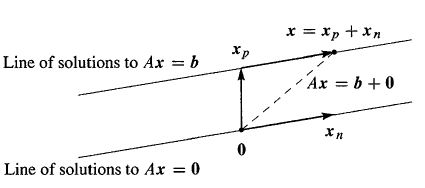
\includegraphics{week2/complete.jpg}
\caption{Complete solution = one particular solution + all nullspace solutions}
\end{figure}
\end{example}
\subsubsection{Row-Echelon Matrices}
Given $m\x n$ rectangular matrix $\bm A$, we can still do Gaussian Elimination to convert $\bm A$ into $\bm U$, where $\bm U$ is of \emph{Row Echelon form}. The whole process could be expressed as:
\[
\bm{PA} = \bm{LDU}.
\]
where $\bm L$ is $m\x m$ \emph{lower triangular} matrix, $\bm U$ is $m\x n$ matrix that is of \emph{row echelon form}.

\begin{example} Here is a $4\x 7$ row echelon matrix with the three pivots $\bm 1$ highlighted in blue:
\[
\bm U = \left[
\begin{array}{@{}ccccccc@{}}
\cellcolor{cyan!50}1&\x&\x&\x&\x&\x&\x\\
0&\cellcolor{cyan!50}1&\x&\x&\x&\x&\x\\
0&0&0&0&0&\cellcolor{cyan!50}1&\x\\
0&0&0&0&0&0&0
\end{array}
\right]
\]
\begin{itemize}
\item
Columns 3,4,5,7 have no pivots, and we say the free variables are $x_3,x_4,x_5,x_7.$
\item
Columns 1,2,6 have pivots, and we say the pivot variables are $x_1,x_2,x_6.$
\end{itemize}
Moreover, we can continue Gaussian Elimination to convert $\bm U$ into $\bm R$ that is of \emph{reduced row echelon form}:
\[
\bm R = \left[
\begin{array}{@{}ccccccc@{}}
\cellcolor{cyan!50}1&0&\x&\x&\x&0&\x\\
0&\cellcolor{cyan!50}1&\x&\x&\x&0&\x\\
0&0&0&0&0&\cellcolor{cyan!50}1&\x\\
0&0&0&0&0&0&0
\end{array}
\right]
\]
\emph{The reduced row echelon matrix $\bm R$ has zeros above the pivots as well as below. Zeros above the pivots come from upward elimination.}
\end{example}
\begin{remark}
Remember the two steps (forward and back elimination) in solving $\bm{Ax} = \bm b$:
\begin{enumerate}
\item
\emph{Forward Elimination} takes $\bm A$ to $\bm U$. (or its reduced form $\bm R$)
\item
\emph{Back Elimination} in $\bm{Ux} = \bm c$ or $\bm{Rx} = \bm d$ produces $\bm x$.
\end{enumerate}
\end{remark}

\subsubsection{Problem Size Analysis}
When faced with $m\x n$ matrix $\bm A$, notice that $\bm m$ refers to the \emph{number of equations}, $\bm n$ refers to the \emph{number of variables}. Assume $\bm r$ denotes \emph{number of pivots}, then we know $\bm r$ is also the \emph{number of pivot variables}, $\bm n-\bm r$ is the \emph{number of free variables}. Finally we have $\bm m-\bm r$ \emph{redundant equations} and $\bm r$ \emph{irredundant equations}. In next lecture, we will introduce the definition for $\bm r$ formally (rank).











\section{Assignment Three}\index{Assignment_Three}
\begin{enumerate}
\item
Check and verify the following:
\begin{enumerate}
\item
If $\bm M=\bm I-\bm u\bm v\trans$, then \[\bm M^{-1}=\bm I+\frac{\bm u\bm v\trans}{1-\bm v\trans\bm u}.\qquad(\bm v\trans\bm u\ne1)\]
\item
If $\bm M=\bm A-\bm u\bm v\trans$, then \[\bm M^{-1}=\bm A^{-1}+\frac{\bm A^{-1}\bm u\bm v\trans\bm A^{-1}}{1-\bm v\trans\bm A^{-1}\bm u}.\qquad(\bm v\trans\bm A^{-1}\bm u\ne1)\]
\item
If $\bm M=\bm I-\bm U\bm V$, where $\bm U\in\mathbb{R}^{n\x m},\bm V\in\mathbb{R}^{m\x n}$, then \[\bm M^{-1}=\bm I_n+\bm U(\bm I_m-\bm V\bm U)^{-1}\bm V.\]
\item
If $\bm M=\bm I-\bm U\bm W^{-1}\bm V$, where $\bm W\in\mathbb{R}^{m\x m},\bm U\in\mathbb{R}^{n\x m},\bm V\in\mathbb{R}^{m\x n}$, then \[\bm M^{-1}=\bm A^{-1}+\bm A^{-1}\bm U(\bm W-\bm V\bm A^{-1}\bm U)^{-1}\bm V\bm A^{-1}.\]
\end{enumerate}
\item
If $\bm A=\bm A\trans$ and $\bm B=\bm B\trans$, which of these matrices are certainly \textit{symmetric}?
\begin{enumerate}
\item
$\bm A^2-\bm B^2$
\item
$(\bm A+\bm B)(\bm A-\bm B)$
\item
$\bm{ABA}$
\item
$\bm{ABAB}$
\end{enumerate}
\item
Strat from LDU decomposition, show that each $n\x n$ matrix $\bm A$ can be factorized into a \textit{triangular} matrix times a \textit{symmetric} matrix.
\item
Let
\[
\bm A=\begin{bmatrix}
5&3\\3&2
\end{bmatrix},\quad\bm B=\begin{bmatrix}
6&2\\2&4
\end{bmatrix},\quad\bm C=\begin{bmatrix}
4&-2\\-6&3
\end{bmatrix}
\]
solve each of the following matrix equations:
\begin{enumerate}
\item
$\bm{Ax}+\bm B=\bm C$
\item
$\bm{XA}+\bm B=\bm C$
\item
$\bm{AX}+\bm B=\bm X$
\item
$\bm{XA}+\bm C=\bm X$
\end{enumerate}
\item
Let $\bm U$ and $\bm R$ be $n\x n$ upper triangular matrices and $\bm T=\bm{UR}$, show that $\bm T$ is also \textit{upper triangular} and that $t_{jj}=u_{jj}r_{jj},j=1,\dots,n.$
\item
Consider the graph
\begin{figure}[H]
\centering
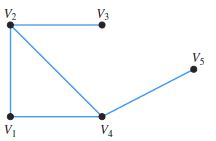
\includegraphics{week2/adj}
\end{figure}
\begin{enumerate}
\item
Determine the adjacency matrix $\bm A$ of the graph.
\item
Compute $\bm A^2$. What do the entries in the first row of $\bm A^2$ tell you about walks of length $2$ that start from $V_1$?
\item
Compute $\bm A^3$. How many walks of length $3$
are there from $V_2$ to $V_3$? How many walks of
length \textit{less than} or \textit{equal} to $3$ are there from $\bm V_2$ to $\bm V_4$?
\end{enumerate}
\end{enumerate}
%\include{week3/Lecture_1}
%\include{week3/Lecture_2}

\chapter{Week3}

\section{Tuesday}\index{week3_Tuesday_lecture}
\subsection{Introduction}
\subsubsection{Motivation of Linear Algebra}
So, we raise the question again, why do we learn LA?
\begin{itemize}
\item
Baisis of AI/ML/SP/etc.\\
In information age, \textit{artificial intelligence, machine learning, structured programming}, and otherwise gains great popularity among researchers. LA is the basis of them, so in order to explore science in modern age, you should learn LA well.
\item
Solving linear system of equations.\\
How to solve linear system of equations efficiently and correctly is the \emph{key} question for mathematicians.
\item
Internal grace.\\
LA is very beautiful, hope you enjoy the beauty of math.
\item
Interview questions.\\
LA is often used for interview questions for phd. The interviewer usually ask difficult questions about LA.
\end{itemize}
\subsubsection{Preview of LA}
The main branches of Mathematics are given below:
\[
\text{mathematics}\begin{cases}
\mbox{Analysis + Calculus} \\
\mbox{Algebra: foucs on structure} \\
\mbox{Geometry}
\end{cases}
\]
All parts of math are based on \emph{axiom systems}. And \emph{LA} is the significant part of \textit{Algebra}, which focus on the linear structure.

\subsection{Review of 2 weeks}
\paragraph{How to solve linear system equations?}
The basic method is \emph{Gaussian Elimination}, and the main idea is \textit{induction} to make simpler equations.
\begin{itemize}
\item
Given one equation $ax=b$, we can easily sovle it:
\[
\begin{array}{ll}
\mbox{If $a=0$, there is no solution}
&
\mbox{otherwise $x=\frac{b}{a}$}.
\end{array}
\]
\item
We could solve $1\times 1$ system. By induction, if we could solve $n\x n$ systems, then we can solve $(n+1)\x(n+1)$ systems.
\end{itemize}

In the above process, math notations is needed:
\begin{itemize}
\item
matrix multiplication
\item
matrix inverse
\item
transpose, symmetric matrices
\end{itemize}
So in first two weeks, we just learn two things:
\begin{itemize}
\item
\textit{linear system could be solved \emph{almost} by G.E.}
\item
\textit{Furthermore, Gaussian Elimination is (almost) LU decomposition.}
\end{itemize}
But there is a question remained to be solved:
\paragraph{How to solve linear singular system equations?}
\begin{itemize}
\item
When does the system have no solution, when does the system have infinitely many solutions? (Note that singular system don't has unique solution.)
\item
If it has infinitely many solutions, how to find and express these solutions?
\end{itemize}
If we express system into matrix form, the question turns into:
\begin{quotation}
How to solve the rectangular?
\end{quotation}

\subsection{Examples of solving equations}

\begin{itemize}
\item
For square case, we often convert the system into $\bm{Ux} = \bm c$, where $\bm U$ is of \textit{row echelon form}.
\item
However, for rectangular case, \textit{row echelon form}(ref) is not enough, we must convert it into \emph{reduced row echelon form}(rref):
\[\bm U\text{(ref)} = \left[
\begin{array}{@{}ccccccc@{}}
\cellcolor{cyan!50}1&0&\x&\x&\x&0&\x\\
0&\cellcolor{cyan!50}1&\x&\x&\x&0&\x\\
0&0&0&0&0&\cellcolor{cyan!50}1&\x\\
0&0&0&0&0&0&0
\end{array}
\right]
\implies
\bm R\text{(rref)} = \left[
\begin{array}{@{}ccccccc@{}}
\cellcolor{cyan!50}1&0&\x&\x&\x&0&\x\\
0&\cellcolor{cyan!50}1&\x&\x&\x&0&\x\\
0&0&0&0&0&\cellcolor{cyan!50}1&\x\\
0&0&0&0&0&0&0
\end{array}
\right]\]
\end{itemize}
\begin{example}
We discuss how to solve \emph{square} matrix of \emph{rref}:
\begin{itemize}
\item
If all rows have nonzero entry, we have:
\[
\begin{bmatrix}
1&&\bigzero&\\
&1&&\\
&&1&\\
&\bigzero&&1
\end{bmatrix}\bm x = \bm c
\implies \bm x = \bm c
\]
\item
But note that \textit{some rows could be all zero}:
\[
\begin{bmatrix}
1&&&\\
&1&&\\
&&1&\\
&&&0
\end{bmatrix}\bm x = \bm c\implies
\begin{cases}
x_1 = c_1\\
x_2 = c_2\\
x_3 = c_3\\
0 = c_4
\end{cases}
\]
So the solution results have two cases:
\begin{itemize}
\item
If $c_4\ne0$, we have no solution of this system.
\item
If $c_4=0$, we have infinitely many solutions, which can be expressed as:
\[
x_{\text{complete}} = \begin{pmatrix}
c_1\\c_2\\c_3\\x_4
\end{pmatrix} = \begin{pmatrix}
c_1\\c_2\\c_3\\0
\end{pmatrix}+x_4\begin{pmatrix}
0\\0\\0\\1
\end{pmatrix}
\]
where $x_4$ could be arbitarary number.
\end{itemize}
\end{itemize}
Hence, for square system, does Gaussian Elimination work?

Answer: Almost, except for the ``pivot=0''case:
\begin{itemize}
\item
All pivots $\ne0\implies$ the system has unique solution.
\item
Some pivots $=0$ (The matrix is singular)
\begin{enumerate}
\item
No solution. (When LHS $\ne$ RHS)
\item
Infinitely many solutions.
\end{enumerate}
\end{itemize}
\end{example}

\subsubsection{
Review of G.E. for Nonsingular case
}
We use matrix to represent system of equations: 
\[
\begin{cases}
a_{11}x_1 + a_{12}x_2 + \dots + a_{1n}x_n = b_1 \\ 
a_{21}x_1 + a_{22}x_2 + \dots + a_{23}x_n = b_2  \\
\dots 	 	\\
a_{m1}x_1 + a_{m2}x_2 + \dots + a_{m3}x_n = b_m  
\end{cases}
\implies
\bm{Ax} = \bm b\]
By postmultiplying $\bm E_{ij}$ or $\bm P_{ij}$, we are essentially doing one step of elimination:
\[
\begin{array}{lll}
\bm E_{ij}\bm A\bm x = \bm E_{ij}\bm b
&
\mbox{or}
&
\bm P_{ij}\bm A\bm x = \bm E_{ij}\bm b
\end{array}
\]
By several steps of elimination, we obtain the final result:
\[
\bm{\hat LPAx} = \bm{\hat LP}\bm b
\]
where $\bm{\hat LPA}$ represents an upper triangular matrix $\bm U$, $\hat L$ is the lower triangular matrix.

 Equivalently, we obtain
\[
\bm{\hat LPA} = \bm U\implies
\bm{PA} = \bm{\hat L}^{-1}\bm U\triangleq\bm{LU}
\]
Hence, Gaussian Elimination is almost the $LU$ decomposition.

\subsubsection{Example for solving rectangular system of rref}
Recall the definition for rref:
\begin{definition}[reduced row echelon form]
Suppose a matrix has $r$ \textit{nonzero} rows, each row has leading $1$ as pivots. If all columns with pivots (call it pivot column) are all zero entries apart from the pivot in this column, then this matrix is said to be \emph{reduced row echelon form}(\emph{rref}).
\end{definition}
Next, we want to show how to solve a rectangular system of rref. Note that in last lecture we study the solution to a rectangular system  is given by:
\[
\bm x_{\text{complete}} =\bm x_p +\bm x_{\text{special}}.
\]

\begin{example}
Solve the system 
\[
\begin{bmatrix}
1&3&0&0\\0&0&1&1\\0&0&0&0
\end{bmatrix}\bm x = \bm c.
\]
\paragraph{Step 1: Find null space} Firstly we solve for $\bm{Rx} = \bm 0$:
\[
\begin{bmatrix}
1&3&0&0\\0&0&1&1\\0&0&0&0
\end{bmatrix}\begin{bmatrix}
x_1\\x_2\\x_3\\x_4
\end{bmatrix} = \begin{bmatrix}
0\\0\\0
\end{bmatrix}\implies \left\{\begin{rgathered}
x_1+3x_2=0\\
x_3+x_4=0
\end{rgathered}\right.
\]

Then we express the \emph{pivot variables} in the form of \emph{free variables.}
\begin{quotation}
Note that the pivot columns in $\bm R$ are column $1$ and $3$, so the pivot variable is $x_1$ and $x_3$. The free variable is the remaining variable, say, $x_2$ and $x_4$.
\end{quotation}
The expressions for $x_1$ and $x_3$ are given by:
\[
\left\{\begin{lgathered}
x_1=-3x_2\\
x_3=-x_4
\end{lgathered}\right.
\]

Hence, all solutions to $\bm{Rx} = \bm 0$ are
\[
\bm x_{\text{special}} = \begin{bmatrix}
-3x_2\\x_2\\-x_4\\x_4
\end{bmatrix} = x_2\begin{bmatrix}
-3\\1\\0\\0
\end{bmatrix} + x_4\begin{bmatrix}
0\\0\\-1\\1
\end{bmatrix}
\]
where $x_2$ and $x_4$ can be taken arbitararily.
\paragraph{Step 2: Find one particular solution to $\bm{Rx} = \bm c$} The trick for this step is to set $x_2=x_4=0$. (\textit{set free variable to be zero and then derive the pivot variable.}):
\[
\begin{bmatrix}
1&3&0&0\\0&0&1&1\\0&0&0&0
\end{bmatrix}\begin{bmatrix}
x_1\\0\\x_3\\0
\end{bmatrix} = \begin{bmatrix}
c_1\\c_2\\c_3
\end{bmatrix}
\implies
\left\{\begin{rgathered}
x_1 =c_1\\
x_3 =c_2\\
0 =c_3
\end{rgathered}\right.
\]
which follows that:
\begin{itemize}
\item
if $c_3 = 0$, then exists particular solution $\bm x_p = \begin{bmatrix}
c_1\\0\\c_2\\0
\end{bmatrix}$;
\item
if $c_3\ne 0$, then $\bm{Rx} = \bm c$ has no solution.
\end{itemize}
\paragraph{Final solution} If assume $c_3= 0$, then all solutions to $\bm{Rx} = \bm c$ are given by:
\[
\bm x_{complete} = \bm x_p + \bm x_{\text{special}} = 
\begin{bmatrix}
c_1\\0\\c_2\\0
\end{bmatrix} + x_2\begin{bmatrix}
-3\\1\\0\\0
\end{bmatrix} + x_4\begin{bmatrix}
0\\0\\-1\\1
\end{bmatrix}
\]
\end{example}
Next we show how to solve a general rectangular:
\newpage
\subsection{How to solve a general rectangular}
For linear system $\bm{Ax} = \bm b$, where $\bm A$ is rectangular, we can solve this system as follows:
\paragraph{Step 1: Gaussian Elimination}
With proper row permutaion (postmultiply $\bm P_{ij}$) and row transformation (postmultiply $\bm E_{ij}$), we convert $\bm A$ into $\bm R$(rref), then we only need to solve $\bm{Rx} = \bm c$.
\begin{example}
The first example is a $3\x 4$ matrix with two pivots:
\[
\bm A = \begin{bmatrix}
1&1&2&3\\2&2&8&10\\3&3&10&13
\end{bmatrix}
\]
Clearly $a_{11}=1$ is the first pivot, then we clear row 2 and row 3 of this matrix:
\[
\bm A
\xLongrightarrow[\bm E_{31} = \begin{bmatrix}
1&0&0\\0&1&0\\-3&0&1
\end{bmatrix}]{\bm E_{21} = \begin{bmatrix}
1&0&0\\-2&1&0\\0&0&1
\end{bmatrix}}
\begin{bmatrix}
1&1&2&3\\0&0&4&4\\0&0&4&4
\end{bmatrix}
\xLongrightarrow[\bm E_{32} = \begin{bmatrix}
1&0&0\\0&1&0\\0&-1&1
\end{bmatrix}]{\bm E_{12} = \begin{bmatrix}
1&-\frac{1}{2}&0\\0&1&0\\0&0&1
\end{bmatrix}}
\begin{bmatrix}
1&1&0&1\\0&0&4&4\\0&0&0&0
\end{bmatrix}\\
\]
\[\implies \begin{bmatrix}
1&1&0&1\\0&0&1&1\\0&0&0&0
\end{bmatrix}\]
If we want to solve $\bm{Ax} = \bm b$, firstly we should convert $\bm A$ into $\begin{bmatrix}
1&1&0&1\\0&0&1&1\\0&0&0&0
\end{bmatrix}$(rref).
\end{example}

Then we should identify \emph{pivot variables} and \emph{free variables}. we can follow the proceed below:
\[
\mbox{pivots}
\implies
\mbox{pivot columns}
\implies
\mbox{pivot variables}
\]
\begin{example}
we want to identify \emph{pivot variables} and \emph{free variables} of $\bm R$: 
\[
\bm R = \left[
\begin{array}{@{}ccccccc@{}}
\cellcolor{cyan!50}1&0&\x&\x&\x&0&\x\\
0&\cellcolor{cyan!50}1&\x&\x&\x&0&\x\\
0&0&0&0&0&\cellcolor{cyan!50}1&\x\\
0&0&0&0&0&0&0
\end{array}
\right]
\]
The pivot are $r_{11},r_{22},r_{36}$. So the pivot columns are column $1,2,6$. So the \textit{pivot variables} are $x_1,x_2,x_6$; the \textit{free variables} are $x_3,x_4,x_5,x_7$.
\end{example}
\paragraph{Step2: Compute null space $N(\bm A)$}
In order to find $N(\bm A)$, it suffices to compute $N(\bm R)$. The space $N(\bm R)$ has $(n-r)$ dimensions, so it suffices to get $(n-r)$ special solutions first:
\begin{itemize}
\item
For each of the $(n-r)$ free variables,
\begin{itemize}
\item
set the value of \emph{it} to be $1$;
\item
set the value of other \emph{free variables} to be 0;
\item
Then solve $\bm{Rx} = \bm 0$ (to get the value of pivot variables) to get the special solution.
\end{itemize}
\begin{example}
Continue with $3\x 4$ matrix example:
\[
\bm R = \begin{bmatrix}
1&1&0&1\\0&0&1&1\\0&0&0&0
\end{bmatrix}\]
We want to find special solutions to $\bm{Rx} = \bm 0$:
\begin{enumerate}
\item
Set $x_2=1$ and $x_4=0$. Solve $\bm{Rx} = \bm 0$, then $x_1=-1$ and $x_3 = 0$. \\Hence one special solution is $y_1 = \begin{bmatrix}
-1\\1\\0\\0
\end{bmatrix}$.
\item
Set $x_2=0$ and $x_4=1$. Solve $\bm{Rx} = \bm 0$, then $x_1=-1$ and $x_3 = -1$. \\Then another special solution is $y_2 = \begin{bmatrix}
-1\\0\\-1\\1
\end{bmatrix}$.
\end{enumerate}
\end{example}
\item
Then $N(\bm A)$ is the collection of linear combinations of these special solutions:
\[
N(\bm A) = \Span(y_1,y_2,\dots,y_{n-r}).
\]
\begin{example}
We continue the example above, when we get all special solutions 
\[
\begin{array}{ll}
y_1 = \begin{bmatrix}
-1\\1\\0\\0
\end{bmatrix}
&
y_2 = \begin{bmatrix}
-1\\0\\-1\\1
\end{bmatrix},
\end{array}
\] 
\emph{the null space contains all linear combinations of the special solutions}:
\[
\bm x_{\text{special}} = \Span(\begin{bmatrix}
-1\\1\\0\\0
\end{bmatrix},\begin{bmatrix}
-1\\0\\-1\\1
\end{bmatrix}) = x_2\begin{bmatrix}
-1\\1\\0\\0
\end{bmatrix} + x_4\begin{bmatrix}
-1\\0\\-1\\1
\end{bmatrix}
\]
where $x_2,x_4$ here could be arbitarary.
\end{example}
\end{itemize}

\paragraph{Step3: Compute a particular solution $\bm x_p$}
The easiest way is to ``read'' from $\bm{Rx} = \bm c$:
\begin{quotation}
\begin{itemize}
\item
\emph{Guarantee the existence of the solution}. Suppose $\bm R\in\mathbb{R}^{m\x n}$ has $r (\le m)$ pivot variables, then it has $(m-r)$ zero rows and $(n-r)$ free variables. For the existence of solutions, the value of entries of $\bm c$ which correspond to zero rows in $\bm R$ must also be zero.
\begin{example}
If $\bm{Rx} = \begin{bmatrix}
1&3&0&2\\0&0&1&4\\\bm 0&\bm 0&\bm 0&\bm 0
\end{bmatrix}\bm x = \bm c = \begin{bmatrix}
c_1\\c_2\\c_3
\end{bmatrix}$, then in order to have a solution, we must let $c_3\ne 0$.
\end{example}
\item
If the condition above is not satisfied, then the system has no solution. Let's preassume the satisfaction of such a condition. To compute a particular solution $\bm x_p$, we set \textit{the value for all \emph{free variables} of $\bm x_p$ to be zero, and the value for the pivot variables are from $\bm c$.} 

More specifically, the first entry in $\bm c$ is exactly the value for the first pivot variable;the second entry in $\bm c$ is exactly the value for the second pivot variable$\dots\dots$, and the remaining entries of $\bm x_p$ are set to be zero.
\begin{example}
If $\bm{Rx} = \begin{bmatrix}
1&3&0&2\\0&0&1&4\\\bm 0&\bm 0&\bm 0&\bm 0
\end{bmatrix}\bm x = \bm c = \begin{bmatrix}
c_1\\c_2\\0
\end{bmatrix}$, we want to compute particular solution 
\[\bm x_p = \begin{bmatrix}
x_1\\x_2\\x_3\\x_4
\end{bmatrix}\]
As we know $x_2,x_4$ are free variable, $x_2=x_4=0$; and $x_1,x_3$ are pivot variable, so we have $\begin{pmatrix}
x_1\\x_3
\end{pmatrix} = \begin{pmatrix}
c_1\\c_2
\end{pmatrix}$.\\
Hence the solution for $\bm{Rx} = \bm c$ is 
\[
\bm x_p=
\begin{bmatrix}
c_1\\0\\c_2\\0
\end{bmatrix}.
\]
\end{example}
\end{itemize}
\end{quotation}
\paragraph{Final step: Obtain complete solutions}
All solution of $\bm{Ax} = \bm b$ are 
\[
\bm x_{\text{complete}} = \bm x_p + \bm x_{\text{special}},
\] 
where $x_{\text{special}}\in N(\bm A)$. Note that $\bm x_p$ is defined in step3, $\bm x_{\text{special}}$ is defined in step2.

However, where does the number $r$ come? $r$ denotes the \emph{rank} of a matrix, which will be discussed in the next lecture.





















%\chapter{Week3}

\section{Thursday}\index{week3_Thursday_lecture}
\subsection{Review}
Last time you may be confused about how to compute $N(\bm A)$ or $y_1,y_2,\dots,y_{n-r}$ (step2). Now let's review the whole steps for solving rectangular bu using block matrix:\\
\begin{itemize}
\item
Firstly, we convert our rref into the form $\begin{bmatrix}
\bm I&\bm B\\\bm 0&\bm 0
\end{bmatrix}$ by switching columns.
\begin{example}
Last time our rref is given by:
\[
\bm R = \begin{bmatrix}
1&3&0&-1\\0&0&1&1\\0&0&0&0
\end{bmatrix}
\]
We notice that column 3 is pivot column, so we can switch it into the second column. (By switching column 2 and column 3):
\[
\bm R\implies \begin{bmatrix}
1&0&3&-1\\0&1&0&1\\0&0&0&0
\end{bmatrix} = \begin{bmatrix}
\bm I&\bm B\\\bm 0&\bm 0
\end{bmatrix}
\]
\end{example}
\item
Then our system equation is translated (We use $3\x 4$ matrix to show the whole process.):
\[
\bm{Rx} = \bm c\implies \begin{bmatrix}
\bm I&\bm B\\\bm 0&\bm 0
\end{bmatrix}\begin{bmatrix}
x_1\\x_2\\x_3\\x_4
\end{bmatrix} = \begin{bmatrix}
c_1\\c_2\\c_3
\end{bmatrix}
\]
\newpage

Because we have changed the columns, so here row $2$ and row $3$ is also switched respectively. And then $x_1$ and $x_2$ are pivot variables, $x_3$ and $x_4$ are free variables. Then we derive:
\[
\implies
\left\{\begin{aligned}
\bm I\begin{bmatrix}
x_1\\x_2
\end{bmatrix}+ \bm B\begin{bmatrix}
x_3\\x_4
\end{bmatrix} &= \begin{bmatrix}
c_1\\c_2
\end{bmatrix}\\
0 &= c_3
\end{aligned}\right.
\]
\item
If $c_3\ne 0$, then there is no solution; next, let's assume $c_3=0$. Then \textit{pivot variables} could be expressed as the form of \textit{free variables}:
\[
\begin{pmatrix}
x_1\\x_2
\end{pmatrix} = \begin{pmatrix}
c_1\\c_2
\end{pmatrix} - \bm B\begin{pmatrix}
x_3\\x_4
\end{pmatrix}
\]
Hence all solutions to $\bm{Rx} = \bm c$ is obtained:
\[
\bm x = \begin{bmatrix}
x_1\\x_2\\x_3\\x_4
\end{bmatrix} = \begin{bmatrix}
x_1\\x_2\\0\\0
\end{bmatrix} + \begin{bmatrix}
0\\0\\x_3\\x_4
\end{bmatrix} = 
\begin{bmatrix}
c_1\\c_2\\0\\0
\end{bmatrix} - \begin{bmatrix}
\bm B\begin{pmatrix}
x_3\\x_4
\end{pmatrix}\\0\\0
\end{bmatrix} +\begin{bmatrix}
0\\0\\x_3\\x_4
\end{bmatrix}
\]
Suppose $-\bm B = \begin{bmatrix}
\bm{\hat y_1}&\bm{\hat y_2}
\end{bmatrix}$, then pivot variables is equivalent to
\[
\implies\begin{pmatrix}
x_1\\x_2
\end{pmatrix} = \begin{pmatrix}
c_1\\c_2
\end{pmatrix}+x_3\bm{\hat y_1} + x_4\bm{\hat y_2}
\]
\item
So the complete solution to the system is

\begin{align}
\bm x &= \begin{pmatrix}
c_1\\c_2\\0\\0
\end{pmatrix} +  \begin{pmatrix}
x_3\bm{\hat y_1} + x_4\bm{\hat y_2}\\0\\0
\end{pmatrix} + \begin{pmatrix}
0\\0\\x_3\\x_4
\end{pmatrix}\\
&=\begin{pmatrix}
c_1\\c_2\\0\\0
\end{pmatrix} +  x_3\begin{pmatrix}
\bm{\hat y_1}\\0\\0
\end{pmatrix}+x_4\begin{pmatrix}
\bm{\hat y_2}\\0\\0
\end{pmatrix} + x_3\begin{pmatrix}
0\\0\\1\\0
\end{pmatrix} + x_4\begin{pmatrix}
0\\0\\0\\1
\end{pmatrix}\\
&=\underbrace{\begin{pmatrix}
c_1\\c_2\\0\\0
\end{pmatrix}}_{\bm x_p}
+\underbrace{x_3\begin{pmatrix}
\bm{\hat y_1}\\1\\0
\end{pmatrix} + x_4\begin{pmatrix}
\bm{\hat y_2}\\0\\1
\end{pmatrix}}_{\bm x_{\text{special}}}
\end{align}                                          
where $x_3$ and $x_4$ could be arbitarary.
\item
Notice that the block matrix is given by:
\[\begin{pmatrix}
\bm{\hat y_1}&\bm{\hat y_2}\\1&0\\0&1
\end{pmatrix}
= \begin{pmatrix}
-\bm B\\\bm I
\end{pmatrix}\implies
\begin{pmatrix}
\bm I&\bm B\\\bm 0&\bm 0
\end{pmatrix}\begin{bmatrix}
-\bm B\\\bm I
\end{bmatrix} = \begin{bmatrix}
-\bm B+\bm B\\\bm 0
\end{bmatrix} = \begin{bmatrix}
\bm 0\\\bm 0
\end{bmatrix}
\]
\end{itemize}
If our rectangular matrix is $m\x n(m>n)$, how to solve it?\\
Answer: Also, we do G.E. to get rref, which will be of the form
\[
\begin{bmatrix}
1&&\\&1&\\&&1\\0&\dots&0
\end{bmatrix}\text{ or }\begin{bmatrix}
1& & & & \\
 &\ddots&&&\\
 & & 1&&\\
 &&&0&\\
 &&&&0\\0&0&0&\dots&0
\end{bmatrix}
\]
\subsection{Remarks on solving linear system equations}
\emph{The two possibilities for linear equations depend on $m$ and $n$:}
\begin{theorem}
Let $m$ denote number of equations, $n$ denote number of variables. For number of solutions for $\bm{Ax} = \bm b$, where $\bm A\in\mathbb{R}^{m\x n}$, we obtain:
\begin{itemize}
\item
$m<n$: either no solution or infinitely many solutions
\item
$m\ge n$: no solution;unique solution ($N(\bm A) =\bm 0$); or infinitely many solutions.
\end{itemize}
\end{theorem}
\begin{proof}[Proofoutline for $m<n$ case:]
Recall we can convert $\bm{Ax} = \bm b$ into $\bm{Rx} = \bm{c}$:
\[
\begin{bmatrix}
1&&&\x&\x\\&\ddots&&\x&\x\\&&1&\x&\x\\0&0&0&0&0\\\dots&&&&\\0&0&0&0&0
\end{bmatrix}\bm x = \begin{bmatrix}
c_1\\\vdots\\c_r\\c_{r+1}\\\vdots\\c_n
\end{bmatrix}
\]
Note that $x_1.x_2.\dots,x_r$ is pivot variables (This is because of column switching). Hence we have $(n-r)$ free variables, thus $N(\bm A)$ is spanned by $(n-r)$ special vectors $y_1,y_2,\dots,y_{n-r}$.\\
Hence we only need to show $n>r$ \textit{given the condition} $n>m$:\\
Obviously, $r\le m$, and we have $n>m$, so we obtain $n>r$.
\end{proof}
So we get the proposition immediately:
\begin{proposition}
For system $\bm{Ax} = \bm b$, where $\bm A\in\mathbb{R}^{m\x n},$ $m<n$,\\
\hspace*{1cm}it either has no solution or infinitely many solutions.
\end{proposition}
\begin{corollary}\label{corollary_infinite_condition}
For system $\bm{Ax} = \bm 0$, where $\bm A\in\mathbb{R}^{m\x n},$ $m<n$,\\
\hspace*{1cm} it always has infinitely many solutions.
\end{corollary}
\newpage

\subsubsection{What is r?}
We ask the question again, what is $r$? Let's see some examples before answering this question.
\begin{example}
If we want to solve system of equations of size $1000$ as the following:
\[
\left\{\begin{aligned}
x_1+x_2&=3\\2x_1+2x_2&=6\\\dots\\1000x_1+1000x_2&=3000
\end{aligned}\right.
\]
It seems very difficult when hearding it has 1000 equations, but the remaining 999 equations could be redundant (They actually don't exist):
\[
\begin{bmatrix}
1&1\\2&2\\\vdots&\vdots\\1000&1000
\end{bmatrix}\implies
\begin{bmatrix}
1&1\\0&0\\\vdots&\vdots\\0&0
\end{bmatrix}
\]
\end{example}
Here we see only one equation $x_1+x_2=3$ is true, the remaining part is not true. So we claim that $r$ is the number of ``true'' equations. But what is the definition for ``true'' equations? Let's discuss the definition for \textit{linear dependence} first.
\subsection{Linearly dependence}
\begin{definition}[linearly dependence]
The vectors $\bm v_1,\bm v_2,\dots,\bm v_n$ in linear space $\bm V$ are \emph{linearly dependent} if there exists $c_1,c_2,\dots,c_n\in\mathbb{R}$ s.t.
\[
c_1\bm v_1+c_2\bm v_2 +\dots+c_n\bm v_n = \bm 0.
\]
In other words, it means one of $v_i$ could be expressed as linear combination of others. When assuming $c_n\ne 0$, we can express $\bm v_n$ as:
\[
\bm v_n = -\frac{c_1}{c_n}\bm v_1-\frac{c_2}{c_n}\bm v_2 -\dots-\frac{c_{n-1}}{c_n}\bm v_{n-1}.
\]
\end{definition}
\begin{definition}[linearly independence]
The vectors $\bm v_1,\bm v_2,\dots,\bm v_n$ in linear space $\bm V$ are \emph{linearly independent} if the two statements are equivalent:
\begin{itemize}
\item
$c_1\bm v_1+c_2\bm v_2 +\dots+c_n\bm v_n = \bm 0$
\item
All scalars $c_1=c_2=\dots=c_n=0$.
\end{itemize}
In other words, if $\bm v_1,\bm v_2,\dots,\bm v_n$ are not \emph{linearly dependent}, they must be \emph{linearly independent}.
\end{definition}
\begin{remark}
Note that \emph{only} in this course, if we say vectors are dependent, we mean they are \emph{linearly} dependent. And we often express \textit{dependent} as \textit{dep.}; we also sometimes express \textit{linearly dependent} as \textit{lin. dep.}; express \textit{linearly independent} as \textit{lin. ind.}
\end{remark}
Here we pick some examples to help you understand lin. dep. and lin. ind.:
\newpage
\begin{example}\qquad\\
\begin{itemize}
\item
$\bm v_1=(1,1)$ and $\bm v_2 = (2,2)$ are \emph{dep.} because
\[
(-2)\x\bm v_1 + \bm v_2 = \bm 0.
\]
\item
The only one vector $\bm v_1=2$ is \emph{ind.} because 
\[
c\bm v_1 = \bm 0
\Longleftrightarrow
c=0.
\]
\item
The only one vector $\bm v_1=0$ is \emph{dep.} because
\[
2\x\bm v_1 = \bm 0
\]
\item
$\bm v_1 = (1,2)$ and $\bm v_2 = (0,0)$ are \emph{dep.} because
\[
0\x\bm v_1 + 1\x\bm v_2 = \bm 0.
\]
\item
The upper triangular matrix $\bm A = \begin{bmatrix}
3&4&2\\0&1&5\\0&0&2
\end{bmatrix}$ has three column vectors:
\[
\bm v_1 = \begin{bmatrix}
3\\0\\0
\end{bmatrix},\bm v_2 = \begin{bmatrix}
4\\1\\0
\end{bmatrix},\bm v_3 = \begin{bmatrix}
2\\5\\2
\end{bmatrix}
\]
$\bm v_1,\bm v_2,\bm v_3$ are \emph{ind.} because
\[
c_1\bm v_1 + c_2\bm v_2 + c_3\bm v_3 = \bm 0
\Longleftrightarrow
c_1=c_2=c_3=0. (\text{Why?})
\]
\end{itemize}
\end{example}
\subsubsection{Relation between \textit{lin.ind.} and \textit{equations}}
The following statements are equivalent:
\begin{itemize}
\item
Vectors $a_1,a_2,\dots,a_n\in\mathbb{R}^{m}$ are dep.
\item
$\exists$ $c_i$ not all zero s.t. $\sum_{i=1}^{n}c_ia_i = \bm 0$.
\item
$\exists$ some $\bm c\ne\bm 0$ s.t.
\[
\bm{Ac} = \left[\begin{array}{c|c|c}
a_1&\dots&a_n
\end{array}\right]\bm c = \bm 0
\]
\end{itemize}
So what if $m<n$, when checking corollary (\ref{corollary_infinite_condition}), we immediately obtain:
\begin{corollary}
When vectors $a_1,a_2,\dots,a_n\in\mathbb{R}^{m}(m<n)$ are dependent, there exists infinitely solutions $c_1,c_2,\dots,c_n$ such that $\sum_{i=1}^{n}c_ia_i = \bm 0$.
\end{corollary}
So we say the true equations are those linearly independent equations.
\newpage

\subsection{Basis and dimension}
\begin{definition}[Basis]
The vectors $v_1,\dots,v_n$ form a \emph{basis} for a vector space $\bm V$ if and only if:
\begin{enumerate}
\item
$v_1,\dots,v_n$ are \emph{linearly independent}.
\item
$v_1,\dots,v_n$ span $\bm V$.
\end{enumerate}
\end{definition}
\begin{example}
In $\mathbb{R}^{3}$, $\begin{bmatrix}
1\\0\\0
\end{bmatrix},\begin{bmatrix}
0\\1\\0
\end{bmatrix},\begin{bmatrix}
0\\0\\1
\end{bmatrix}$ form a basis.\\
$\begin{bmatrix}
1\\0\\0
\end{bmatrix}$ is not a basis, since it doesn't span $\mathbb{R}^{3}$.\\
$\begin{bmatrix}
1\\0\\0
\end{bmatrix},\begin{bmatrix}
0\\1\\0
\end{bmatrix},\begin{bmatrix}
0\\0\\1
\end{bmatrix},\begin{bmatrix}
2\\0\\0
\end{bmatrix}$ don't form a basis, since they don'y linearly independent.\\
$\begin{bmatrix}
1\\0\\0
\end{bmatrix},\begin{bmatrix}
1\\2\\3
\end{bmatrix},\begin{bmatrix}
2\\1\\3
\end{bmatrix}$ form a basis.
\end{example}
We feel that the number of vectors for basis of $\mathbb{R}^{3}$ is always 3, is this a coincidence? The theorem below gives the answer.
\begin{theorem}\label{theorem_3.2}
If $v_1,v_2,\dots,v_m$ is a basis; $w_1,w_2,\dots,w_n$ is a basis for the same vector space $\bm V$, then $n=m$.
\end{theorem}
In order to proof it, let's try simple case first:
\begin{proof}[proofoutline.]\qquad\\

\begin{itemize}
\item
Let's consider $\bm V = \mathbb{R}$ case first:\\
For $\mathbb{R}$, 1 forms a basis.\\
Given any two vectors $x$ and $y$, they are not a basis for $\mathbb{R}$. It is because that
\begin{itemize}
\item
if $x=0$ or $y=0$, they are not ind.
\item
otherwise, $y = \frac{y}{x}\x x\implies \frac{y}{x}\x x + (-1)\x y = 0$. So they are not ind.
\end{itemize}\item
Then we consider $\bm V = \mathbb{R}^3$ case:\\
For $\mathbb{R}^3$, $\begin{bmatrix}
1\\0\\0
\end{bmatrix},\begin{bmatrix}
0\\1\\0
\end{bmatrix},\begin{bmatrix}
0\\0\\1
\end{bmatrix}$ is a basis.\\
We want to show if $v_1,v_2,\dots,v_m$ is a basis, then $m=3$.



\begin{itemize}
\item
Let's proof $m=4$ is impossible ($4$ vectors in $\mathbb{R}^{3}$ cannot be a basis.):\\
We only need to show for $\forall a_1,a_2,a_3,a_4\in\mathbb{R}^{3}$ they must be dep.\\
$\Longleftrightarrow$$\bm{Ax} = \bm 0$ has nonzero solutions, where $\bm A = \left[\begin{array}{c|c|c|c}
a_1&a_2&\dots&a_4
\end{array}\right]\in \mathbb{R}^{3\x 4}$. \\
By corollary (\ref{corollary_infinite_condition}), it is obviously true.
\item
The same argument could show any basis for $\mathbb{R}^{3}$ satisfies $m\le 3$.
\item
Then let's prove $m=2$ is impossible (2 vectors in $\mathbb{R}^{2}$ cannot be a basis):\\
We only need to show for $\forall a_1,a_2\in \mathbb{R}^{3}$, they cannot span the whole space.\\
If this is not true, then $\bm{Ax} = \bm b$ must have solution, where $\bm A = \left[\begin{array}{c|c}
a_1&a_2
\end{array}\right]\in \mathbb{R}^{3\x 2}$.\\
However, this kind matrix may have no solution, which forms a contradiction.
\item
The same arugment could show any basis for $\mathbb{R}^{3}$ satisfies $m\ge 3$.
\end{itemize}
\item
The same arugment could show any basis for $\mathbb{R}^{n}$ satisfies $m=n$.
\item
Next, let's consider general vector space:\\
We assume $n<m$ (contradiction).\\
We have known $v_1,\dots,v_n$ is a basis, our goal is to show $w_1,\dots,w_m$ cannot form a basis.\\
$\Leftarrow\exists$ $\bm c = \begin{bmatrix}
c_1&c_2&\dots&c_m
\end{bmatrix}\trans\ne\bm 0$ s.t.
\begin{equation}\label{combination}
c_1w_1+c_2w_2+\dots+c_mw_m = 0.
\end{equation}
Moreover, we can express $w_1,\dots,w_m$ in form of $v_1,\dots,v_n$:
\begin{equation}\label{basis_for_w}
\left\{\begin{aligned}
w_1 &= a_{11}v_1 +\dots+a_{1n}v_n\\
\dots\\
w_m &= a_{m1}v_1 +\dots + a_{mn}v_n
\end{aligned}\right.
\end{equation}
By (\ref{basis_for_w}), we can write (\ref{combination}) as:
\[
\begin{aligned}
0 &= \sum_{j=1}^{m}c_jw_j\\
  &= \sum_{j=1}^{m}c_j(\sum_{i=1}^{n}a_{ji}v_i)\\
  &= \sum_{j=1}^{m}\sum_{i=1}^{n}c_ja_{ji}v_i\\
  &= \sum_{i=1}^{n}\sum_{j=1}^{m}c_ja_{ji}v_i\\
  &= \sum_{i=1}^{n}v_i\x(\sum_{j=1}^{m}c_ja_{ji})\\
  &= v_1\x(\sum_{j=1}^{m}c_ja_{j1}) + v_2\x(\sum_{j=1}^{m}c_ja_{j2}) +\dots +v_n\x(\sum_{j=1}^{m}c_ja_{jn})
\end{aligned}
\]
So, in order to let LHS=0, we only need to let each of RHS=0, more specifically, we only need to let $
\sum_{j=1}^{m}c_ja_{j1} = \sum_{j=1}^{m}c_ja_{j2} = \dots = \sum_{j=1}^{m}c_ja_{jn} = 0.$
\\To write it into matrix form, we only need to let system $\bm A\trans \bm c = \bm 0$ has solution. \\where $\bm A = \begin{bmatrix}
a_{ij}
\end{bmatrix}_{1\le i\le m;1\le j\le n}$ and $\bm c = \begin{bmatrix}
c_1&c_2&\dots&c_m
\end{bmatrix}\trans$.\\
By corollary (\ref{corollary_infinite_condition}), since $\bm A\trans$ is $n\x m$ matrix where $n<m$, it has infinitely nonzero solution.
\end{itemize}
\end{proof}
During the proof, we face two difficulties:
\begin{enumerate}
\item
For arbitararily $\bm V$, we write a concrete form to express $w_1,w_2,\dots,w_m$.
\item
We write matrix form to express $\sum_{j=1}^{m}c_ja_{j1} = \sum_{j=1}^{m}c_ja_{j2} = \dots = \sum_{j=1}^{m}c_ja_{jn} = 0.$
\end{enumerate}
Next since all basis contains the same number of vectors, we can define the number of vectors to be dimension:
\begin{definition}[Dimension]
The \emph{dimension} for a vector space is the number of vectors in a basis for it.
\end{definition}
\begin{remark}
Remember that vector space $\{0\}$ has dimension $0$.\\In order to denote the dimension for a given vector space $\bm V$, we often write it as dim($\bm V$).
\end{remark}
\begin{example}
\begin{itemize}
\item
$\mathbb{R}^{n}$ has dimension $n$.
\item
$\{\text{All $m\x n$ matrix}\}$ has dimension $m\cdot n$.
\item
$\{\text{All $n\x n$ symmetric matrix}\}$ has dimension $\frac{n(n+1)}{2}$.
\item
Let $\bm P$ denote the vector space of all polynomials $f(x) = a_0+a_1x+\dots+a_nx^n$.\\
dim($\bm P$)$\ne 3$ since $1,x,x^2,x^3$ are ind.\\
The same argument can show dim($\bm P$) is not equal to any real number, so dim($\bm P$)=$\infty$
\end{itemize}
\end{example}
Human beings often ask a question: for a line and a plane, which is bigger?
\begin{enumerate}
\item
Does plane has more point than a line?\\
No, Cantor syas they have the same ``number'' of points by constructing a one-to-one mapping.\\
Furthermore, $\mathbb{R},\mathbb{R}^2,\dots,\mathbb{R}^n$ has the same number of points.
\item
However, the plane has bigger dimension than a line. So from this point of view, a plane is bigger than a line.
\end{enumerate}
You should know some common knowledge for dimension:
\begin{enumerate}
\item
Programmer lives in $\bm 2$ dimension world. (They only live with binary.)
\item
Engineer lives in $\bm 3$ dimension world. (They only live with enign.)
\item
Physician lives in $\bm 4$ dimension world. (They discuss time.)
\item
String theories states that our world is $\bm 11$ or $\bm 26$ dimension, which has been proved by Qingshi Zhu.
\item
For 3-body, they can perform dimension attack on you.
\end{enumerate}
\subsubsection{What is rank?}
Finally let's answer the question: What is rank?\\
rank=dimension of row space of a matrix.\\
We will discuss it next lecture.























\section{Friday}\index{week3_Friday_lecture}
\subsection{Review}
\begin{proposition}\label{solution_for_undetermined_system}
Undetermined system $\bm{Ax} = \bm b (m<n\text{ or number of equations < number of unknowns})$ has no solution or infinitely many solutions.
\end{proposition}
We want to understand the meaning of rank: number of ''true'' equations. \\Then we introduce definition of \textit{linearly independence} and \textit{linearly dependence.}\\
Dependence has relation with system:
\begin{proposition}
$\bm{Ax} = \bm 0$ has nonzero solutions if and only if the column vectors of $\bm A$ are dep.
\end{proposition}
Combining it with proposition  (\ref{solution_for_undetermined_system}) we derive the corollary:
\begin{corollary}
Any $(n+1)$ vectors in $\mathbb{R}^{n}$ are dep.
\end{corollary}
\begin{proposition}
Undetermined system $\bm{Ax} = \bm b (m\ge n\text{ or number of equations $\ge$ number of unknowns})$ may have no solution or unique solution or infinitely many solutions.
\end{proposition}
From this proposition we derive the corollary immediately:
\begin{corollary}
Any $(n-1)$ vectors in $\mathbb{R}^{n}$ cannot span the whole space.
\end{corollary}
Then we introduce the definition of basis:
\begin{definition}[Basis]
A set of ind. vectors that span this space is called the \emph{basis} of this space.
\end{definition}
Then we introduce a theorem says \emph{All basis of a given vector space have the same size.}\\
Hence we introduce \emph{dimension} to denote the \textit{number of vectors in a basis.}
\subsection{More on basis and dimension}
The basis of a given vector space has to satisfy two constraints:
\[
\underbrace{\text{lin. ind.}}_{\text{not too many}}+\underbrace{\text{ span the space}}_{\text{not too few}}
\]
The \emph{lin. ind.} constraint let the size of basis not too many. For example, if given $1000$ vectors of $\mathbb{R}^{3}$, they are very likely to be dep. \\
\emph{Spanning the space} let the size of basis not too few. For example, given only $3$ vectors of $\mathbb{R}^{100}$, they cannot span the whole space obviously.\\
We claim: \begin{align*}
\text{A basis }&=\text{ maximal ind. set}\\
&=\text{ minimal spanning set}
\end{align*}
\begin{definition}[spanning set]
$v_1,v_2,\dots,v_n$ is the spanning set of $\bm V$ iff. $\bm V = \text{span}\{v_1,v_2,\dots,v_n\}$.
\end{definition}
\begin{example}
$v_1 = \begin{pmatrix}
1\\2\\1
\end{pmatrix}$ is not a basis of $\mathbb{R}^{3}$.\\
We can add $v_2 = \begin{pmatrix}
1\\0\\0
\end{pmatrix}$, which is ind. of $v_1$. But they still don't form a basis.\\
Then we add one more vector $v_3 = \begin{pmatrix}
0\\1\\0
\end{pmatrix}$, then $v_1,v_2,v_3$ form a basis of $\mathbb{R}^{3}$.
\end{example}
\begin{theorem}\label{theorem_3.3}
Let $\bm V$ be a space of dimension $n>0$, then
\begin{enumerate}
\item
Any set of $n$ ind. vectors span $\bm V$.
\item
Any $n$ vectors that span $\bm V$ are ind.
\end{enumerate}
\end{theorem}

Here I list the proof outline, you should follow the direction to prove it in detail.
\begin{proof}[proofoutline.]\qquad\\
\begin{enumerate}
\item
Suppose $v_1,v_2,\dots,v_n$ are ind. and $v$ is arbitarary vector in $\bm V$. Firstly, show that $v_1,v_2,\dots,v_n,v$ is dep. Thus derive the equation $c_1v_1+c_2v_2+\dots+c_{n}v_n+c_{n+1}v = \bm 0$. Argue that scalar $c_{n+1}\ne 0$. Then express $v$ in form of $v_1,v_2,\dots,v_n$. It follows that $v_1,v_2,\dots,v_n$ span $\bm V$.
\item
Suppose $v_1,v_2,\dots,v_n$ span $\bm V$. Assume $v_1,v_2,\dots,v_n$ are dep. Then show that $v_n$ could be written as form of other $(n-1)$ vectors, it follows that $v_1,v_2,\dots,v_{n-1}$ still span $\bm V$. If $v_1,v_2,\dots,v_{n-1}$ are also dep, we can continue eliminating one vector. We continue this way until we get an ind. spanning set with $k<n$ elements, which contradicts dim($\bm V$)$=n$. Therefore, $v_1,v_2,\dots,v_n$ must be ind.\end{enumerate}
\end{proof}
\enlargethispage{1cm}
\begin{example}\label{span_dimension_three}
$\begin{pmatrix}
1\\1\\2
\end{pmatrix},\begin{pmatrix}
2\\1\\3
\end{pmatrix},\begin{pmatrix}
1\\3\\2
\end{pmatrix}$ are ind. $\implies$ they span $\mathbb{R}^{3}$.
\end{example}
\newpage
\subsubsection{Clarification of dimension}
Firstly, we need to understand ``set'':
\begin{enumerate}
\item
$P\triangleq\{\text{All polynomials}\} = \text{span}\{1,x,x^2,\dots\}\implies \text{dim}(P)=\infty$.
\item
$P_3\triangleq\{\text{All polynomials with degree $\le$ 3}\} = \text{span}\{1,x,x^2,x^3\}\implies \text{dim}(P)=4$.
\item
$Q\triangleq\text{span}\{x^2,1+x^3+x^{10},x^{300}\}\implies \text{dim}(Q) = 3.$
\end{enumerate}
\begin{remark}
dim of space $\ne$ dim of the space it lives in.\\
For example, the line in $\mathbb{R}^{100}$ has dim $1$.
\end{remark}
\subsection{What is rank?}
rank is \textit{the number of nonzero pivots of rref of A.}
\begin{example}\qquad\\
\[
\bm A = \begin{bmatrix}
1&3&3&4\\2&6&9&7\\-1&-3&3&4
\end{bmatrix}
\xLongrightarrow{\text{row transform}}
\bm U = \begin{bmatrix}
1&3&0&-1\\0&0&1&1\\0&0&0&0
\end{bmatrix}
\]
$\bm U$ has two pivots, hence rank($\bm A$) = rank($\bm U$) = 2.
\end{example}
However, the definition for rank is too complicated, can we define rank of $\bm A$ directly?\\
\emph{Key question: What quantity is not changed under row transformation?}\\
\textit{Answer: }Dimension of row space.
\begin{definition}[column space]
The \emph{column space} of a matrix is the subspace of $\mathbb{R}^{n}$ spanned by the columns.\\
In other words, suppose $\bm A = \left[\begin{array}{c|c|c}
a_1&\dots&a_n
\end{array}\right]$, the column space is given by
\[
\text{col}(\bm A) = \text{span}\{a_1,a_2,\dots,a_n\}.
\]
\end{definition}
\begin{definition}[row space]
The \emph{row space} of a matrix is the subspace of $\mathbb{R}^{n}$ spanned by the rows.\\
The \emph{row space} of $\bm A$ is $\text{col}(\bm A\trans)$, it is the column space of $\bm A\trans$.\\
In other words, suppose $\bm A = \left[\begin{array}{c}
a_1\\
\hline
\dots\\
\hline
a_n
\end{array}\right]$, the row space is given by
\[
\row(\bm A) = \Span\{a_1,a_2,\dots,a_n\}.
\]
\end{definition}
\begin{proposition}\label{row_transformation}
Row transforamtion doesn't change the row space
\end{proposition}
\begin{proof}
After row transformation, \textit{new rows are linear combinations of old rows.} \\Hence we have $\row(new rows) \subset\row(old rows)$.\\
Assuming $\bm A\xLongrightarrow{\text{Row Transfom}}\bm B$, then we have $\row(\bm B)\subset\row(\bm A)$.\\
Since row transformations are invertible, we also have $\bm B\xLongrightarrow{\text{Row Transfom}}\bm A$, hence we have $\row(\bm A)\subset\row(\bm B)$.\\
Hence we obtain $\row(\bm B)=\row(\bm A)$.
\end{proof}
\newpage
Hence $\rank(\bm A) = \text{pivots of $\bm U$} = \dim(\row(\bm U)) = \dim(\row(\bm A))$.\\
Hence we have a much simpler definition for rank:
\begin{definition}[rank]
The \emph{dimension of the column space} is the \emph{rank of a matrix}.
\end{definition}
In example (\ref{span_dimension_three}), we find $\dim(\row(\bm A)) = \dim(\col(\bm A)) = 2$, is this a coincidence? \textit{The fundamental theorem of linear algebra} gives this answer:
\begin{theorem}\label{column_rank_row_rank}
The row space and column space both have dimension $\bm r$. Sometimes we call $\dim(\col(\bm A))$ as \textit{column rank}, we call $\dim(\row(\bm A))$ as \textit{row rank}. \\Thus it says \textit{column rank=row rank= rank}.\\
In other words, $\dim(\row(\bm A)) = \dim(\col(\bm A)).$
\end{theorem}
Let's discuss an example to have an idea of proving it.
\begin{example}
\qquad\\
\[
\bm A = \begin{bmatrix}
1&3&3&4\\2&6&9&7\\-1&-3&3&4
\end{bmatrix}
\xLongrightarrow{\text{row transform}}
\bm U = \begin{bmatrix}
1&3&0&-1\\0&0&1&1\\0&0&0&0
\end{bmatrix}
\]
We notice that \emph{column rank of $\bm A =\bm 2$} and \emph{column rank of $\bm U =\bm 2$}.\\
Why do they have the same \emph{column space dimension}?\\
\begin{itemize}
\item
\textit{Wrong reason: }''$\bm A$ and $\bm U$ has the same column space''. This is false. For example, the first column of $\bm A$ is $\begin{pmatrix}
1\\2\\-1
\end{pmatrix}\notin\col(\bm U)$. The column spaces of $\bm A$ and $\bm U$ are \emph{different}, but the dimension of them are the \emph{same}----equal to 2.
\item
\textit{Right reason: }The \emph{same} combinations of the columns are zero (or nonzero) for $\bm A$ and $\bm U$. Say it in another way: $\bm{Ax} = \bm 0$ iff. $\bm{Ux} = \bm 0$. In other words, the $r$ pivot columns(of both) are independent; the $(n-r)$ free columns(of both) are dependent. \\
For example, for $\bm U$, column $1$ and $3$ are ind.(pivot columns); column $2$ and $4$ are dep.(free columns).\\
For $\bm A$, column $1$ and $3$ are also ind.(pivot columns); column $2$ and $4$ are also dep.(free columns).
\end{itemize}
\end{example}
We will show \emph{Row transformation doesn't change ind. relations of columns.}
\begin{proposition}
Suppose matrix $\bm A$ is converted into $\bm B$ by row transformation. If a set of columns of $\bm A$ are ind. then so are corresponding columns of $\bm B$.
\end{proposition}
\begin{proof}
Assume $\bm A = \left[\begin{array}{c|c|c}
a_1&\dots&a_n
\end{array}\right], \bm B = \left[\begin{array}{c|c|c}
b_1&\dots&b_n
\end{array}\right]$.\\
Without loss of generality (We often denote it as ``WLOG''), we assume $a_1,a_2,\dots,a_k$ are ind.(We can achieve it by switching columns.)\\
We define $\bm{\hat{A}} = \left[\begin{array}{c|c|c}
a_1&\dots&a_k
\end{array}\right],\bm{\hat{B}} = \left[\begin{array}{c|c|c}
b_1&\dots&b_k
\end{array}\right]$.\\
\begin{enumerate}
\item
Notice that $\bm{\hat{A}}$ could be converted into $\bm{\hat{B}}$ by row transformation.\\
Hence $\bm{\hat{A}x}=\bm 0$ and $\bm{\hat{B}x}=\bm 0$ has same solutions.
\item
On the other hand, $a_1,a_2,\dots,a_k$ are ind. columns.\\
Hence $\bm{\hat{A}x}=\bm 0$ has only zero solution.
\end{enumerate}
Combining (1) and (2), $\bm{\hat{B}x}=\bm 0$ has only zero solution. Hence $b_1,b_2,\dots,b_k$ are ind.
\end{proof}
\newpage
Thus we can answer why $\bm A$ and $\bm U$ has the same column space dimension:
\begin{proposition}\label{column_rank}
Row transformation doesn't change the column rank.
\end{proposition}
\begin{proof}
Assume $\bm A\xLongrightarrow{\text{row transform}}\bm B$.\\
Assume $\dim(\col(\bm A)) = r$, then we pick $r$ ind. columns if $\bm A$. After row transformation, they are still ind. Hence $\dim(\col(\bm B))\ge r = \dim(\col(\bm A))$.\\
Since row transformations are invertible, we get $\bm B\xLongrightarrow{\text{row transform}}\bm A$.\\ Similarly, $\dim(\col(\bm A))\ge \dim(\col(\bm B))$.\\
Hence $\dim(\col(\bm A))= \dim(\col(\bm B))$.
\end{proof}
Thus using proposition (\ref{row_transformation}) and (\ref{column_rank}) we can proof theorem (\ref{column_rank_row_rank}):
\begin{proof}[Proof for theorem \ref{column_rank_row_rank}]
Assume $\bm A\xLongrightarrow{\text{row transform}}\bm U$(rref).\\
\begin{itemize}
\item
Proposition $(\text{\ref{row_transformation}})\implies \dim(\row(\bm A) = \dim(\row(\bm U))$.
\item
Proposition $(\text{\ref{column_rank}})\implies \dim(\col(\bm A) = \dim(\col(\bm U))$.
\item
Notice that $\dim(\row(\bm U))$ denotes number of pivots, $\dim(\col(\bm U))$ denotes number of pivot columns. Obviously, $\dim(\row(\bm U))=\dim(\col(\bm U))$.
\end{itemize}
Hence $\dim(\row(\bm A))=\dim(\col(\bm A))$.
\end{proof}
\begin{remark}
$\dim(\row(\bm U))$ denotes number of pivots, actually, it denotes the number of ``true'' equations. $\dim(\col(\bm U))$ denotes the number of pivot columns, actually, it denotes the number of ``true'' variables.\\
\emph{Theorem \ref{column_rank_row_rank} implies number of ``true'' equations should equal to number of ``true'' variables.}
\end{remark}
\subsubsection{What is null space dimension?}
Assume the system $\bm{Ax}=\bm b$ has $n$ variables.\\
\emph{Number of pivot varibales + Number of free variables = $\bm n$}.
\[
\implies \rank(\bm A) + \rank(N(\bm A)) = n
\]
where $\rank(\bm A) = \dim(\col(\bm A))$.\\
$\bm b\in\col(\bm A)$ iff. $\bm{Ax} = \bm b$ for some $\bm x$.\\
Hence $\col(\bm A)$ denotes all possible vectors in the form $\bm{Ax}$. Hence we call $\col(\bm A)$ as ``\emph{range space}'' of $\bm A$, which is denoted as range($\bm A$).\\
Finally we have $\dim(\text{range($\bm A$)}) + \dim(N(\bm A)) = n$.
\begin{proposition}
If $\bm{Ax} = \bm b$ has at least one solution, then $\rank(\bm A) = \rank(\begin{bmatrix}
\bm A&\bm b
\end{bmatrix})$.
\end{proposition}
\begin{example}
If $\bm A = \begin{bmatrix}
a_1&a_2&a_3
\end{bmatrix}$, if $\bm{Ax} = \bm b$ has at least one solution, then $\rank(\begin{bmatrix}
a_1&a_2&a_3
\end{bmatrix}) = \rank(\begin{bmatrix}
a_1&a_2&a_3&b
\end{bmatrix})$.
\end{example}
\begin{proof}[Proofoutline.]
\[
\bm{Ax} = \bm b\Longleftrightarrow \bm b\in\col(\bm A)
\]
Hence $\bm b$ is the linear combination of columns of $\bm A$. So Adding one more column $\bm b$ doesn't change the dimension of $\col(\bm A)$. Hence $\rank(\bm A) = \rank(\begin{bmatrix}
\bm A&\bm b
\end{bmatrix})$.
\end{proof}
\begin{proposition}
If $\rank(\bm A)\le n-1$ for $m\x n$ matrix $\bm A$, then $\bm{Ax} = \bm b$ has no or infinitely many solutions.
\end{proposition}
\begin{proof}[Proofoutline.]
\[
\dim(\col(\bm A))+\dim(N(\bm A)) = n
\implies \dim(N(\bm A))\ge 1
\]
So we have special solution for $\bm{Ax} = \bm b$. For particular solution, if it doesn't exist, then we have no solution, otherwise we have infinitely many solutions.
\end{proof}
\begin{definition}[Full Rank]
For $m\x n$ matrix $\bm A$, if $\rank(\bm A) = \min(m,n)$, then we say $\bm A$ is \emph{full rank}.
\end{definition}
\begin{theorem}
For $n\x n$ matrix $\bm A$, it is invertible iff. $\rank(\bm A) = n$.
\end{theorem}
\begin{proof}\qquad\\
\textit{Sufficiency.    }Assume $\rank(\bm A)=r<n$, then by row transformation, we can convert $\bm A$ into $\bm U = \begin{bmatrix}
\bm I_{r}&\bm B\\\bm 0&\bm 0
\end{bmatrix}$(rref), where $\bm B$ is $r\x(n-r)$ matrix. We can represent the process in matrix notation:
\[
\bm P\bm A = \bm U(\text{rref})
\]
$\bm P$ is the product of row transformation matrix, which is obviously invertible.\\
Since $\bm A$ is invertible, we let $\bm A^{-1} = \begin{bmatrix}
\bm C_{1}\\\bm C_{2}
\end{bmatrix}$, where $\bm C_{1}$ is an $r\x n$ matrix. Hence 
\[
\bm P = \bm P\bm I_{n}=\bm P(\bm A\bm A^{-1}) = (\bm{PA})\bm A^{-1} = \bm U\bm A^{-1} = \begin{bmatrix}
\bm I_{r}&\bm B\\\bm 0&\bm 0
\end{bmatrix}\begin{bmatrix}
\bm C_{1}\\\bm C_{2}
\end{bmatrix} = \begin{bmatrix}
\bm C_{1}+\bm B\bm C_{2}\\\bm 0
\end{bmatrix}
\]
Since $\bm P$ has $(n-r)$ rows as zero rows, so it is not invertible, which makes contradiction.\\
\textit{Necessity.   }If $\bm A$ is full rank, then it has $n$ pivots, then by row transformation we can convert it into $\bm I$(rref). We can represent this process in matrix notation:
\[
\bm P\bm A = \bm I
\]
where $\bm P$ is the product of row transformation matrix. Hence $\bm P$ is the left inverse of $\bm A$, $\bm A$ is invertible.
\end{proof}
\subsubsection{Matrices of rank 1}
\begin{example}\[
\bm A = \begin{bmatrix}
2&1&1\\4&2&2\\8&4&4\\-2&-1&-1
\end{bmatrix}\xlongequal{\bm v\trans = \begin{bmatrix}
2&1&1
\end{bmatrix}}\begin{bmatrix}
\bm v\trans\\2\bm v\trans\\4\bm v\trans\\-\bm v\trans
\end{bmatrix} = \begin{bmatrix}
1\\2\\4\\-1
\end{bmatrix}\bm v\trans\xlongequal{\bm u=\begin{bmatrix}
1&2&4&-1
\end{bmatrix}\trans}\bm u\bm v\trans
\]
Here $\rank(\bm A) = 1$.
\end{example}
\begin{proposition}
Every rank 1 matrix $\bm A$ has the form $\bm A = \bm u\bm v\trans = \text{column vector}\x\text{row vector}$.
\end{proposition}
\newpage
\begin{proof}
We set $\bm A = \begin{bmatrix}
\bm c_1\\\bm c_2\\\vdots\\\bm c_n
\end{bmatrix}$, where $\bm c_i$ is row vector.
WLOG, we set $\bm c_1\ne\bm 0$ and $\bm c_1 = \begin{pmatrix}
a_1b_1&a_1b_2&\dots&a_1b_n
\end{pmatrix}$, where $a_1\ne0,b_i(i=1,\dots,n)$ are not all zero.\\
Since $\rank(\bm A) = 1$, we have $\dim(\row(\bm A)) = 1$. Hence $\bm c_i$ is dep. with $\bm c_1$. So we set $b_i = \frac{a_i}{a_1}$ for $i=1,2,\dots,n$. Thus we construct the form of $\bm A$:
\[
\bm A = \begin{bmatrix}
a_1b_1&a_1b_2&\dots&a_1b_n\\
a_2b_1&a_2b_2&\dots&a_2b_n\\
\vdots&\vdots&&\vdots\\
a_nb_1&a_nb_2&\dots&a_nb_n\\
\end{bmatrix} = \begin{bmatrix}
a_1\\a_2\\\vdots\\a_n
\end{bmatrix}\begin{bmatrix}
b_1&b_2&\dots&b_n
\end{bmatrix}
\]
\end{proof}
Question: What about the form of rank 2?

\textit{Enjoy midterm!}\\

\includegraphics[width =10cm]{do_it}





















\section{Assignment Four}\index{Assignment_Four}
\begin{enumerate}
\item
Let
\[
\bm A=\begin{bmatrix}
1&2&3&1&-3\\2&5&5&4&9\\3&7&8&5&6
\end{bmatrix}
\]
\begin{enumerate}
\item
Compute the \textit{reduced row echelon form} $\bm U$ of $\bm A$.
\item
Compute all solutions of $\bm{Ax}=\bm b$, where $\bm b=\begin{bmatrix}
1&1&2
\end{bmatrix}\trans.$
\item
Compute all solutions of $\bm{Ax}=\bm b$, where $\bm b=\begin{bmatrix}
b_1&b_2&b_3
\end{bmatrix}\trans.$\\
Note:Identify when there is \textit{no solution}, and when the solution \textit{exists}, write down all solutions in terms of $b_1,b_2,b_3$.
\end{enumerate}
\item
In each of the following, determine the \textit{dimension} of the space:
\begin{enumerate}
\item
$\Span\left\{
\begin{pmatrix}
1\\-2\\2
\end{pmatrix},\begin{pmatrix}
2\\-2\\4
\end{pmatrix},\begin{pmatrix}
-3\\3\\6
\end{pmatrix}
\right\};$
\item
$\col(\bm A)$, where $\bm A=\begin{bmatrix}
1&-2&3&2\\-1&2&-2&-1\\2&-4&5&3
\end{bmatrix};$
\item
$N(\bm B)$, where $\bm B=\begin{bmatrix}
1&3&2\\2&1&4\\4&7&8
\end{bmatrix};$
\item
$\Span\{(x-2)(x+2),x^2(x^4-2),x^6-8\};$
\item
$\Span\{5,\cos 2x,\cos^2 x\}$ as a \textit{subspace} of $C[-\pi,\pi].$\\
$C[-\pi,\pi]$ denotes the space of \textit{continuous functions defined on the domain $C[-\pi,\pi].$}
\end{enumerate}
\item
Let $\bm A$ be an $6\x n$ matrix of rank $r$. For each pair of values of $r$ and $n$ below, how many solutions could one have for the linear system $\bm{Ax}=\bm b$? Explain your answers.
\begin{enumerate}
\item
$n=7,r=5;$
\item
$n=7,r=6;$
\item
$n=5,r=5.$
\end{enumerate}
\item
Prove the following proposition:\\
Let $\bm V$ be a vector space of dimension $n>0$, then
\begin{enumerate}
\item
Any set of n \textit{linearly independent} vectors in $\bm V$ form a basis.
\item
Any set of $n$ vectors that span $\bm V$ form a basis.
\end{enumerate}
\textit{Hint: refer to theorem(\ref{theorem_3.3})}
\item
\begin{enumerate}
\item
Assume $\bm U.\bm V$ are subspaces of a vector space $\bm W$.\\
Define $\bm U+\bm V=\{u+v|u\in\bm U,v\in\bm V\}$, i.e. each vector in $\bm U+\bm V$ is the sum of one vector in $\bm U$ and one vector in $\bm V$.\\
Prove that $\bm U+\bm V$ is a subspace of $\bm W$.
\item
Prove the intersection $\bm U\cap\bm V=\{x|x\in\bm U\text{ and }x\in\bm V\}$ is also a subspace of $\bm W.$
\item
In $\mathbb{R}^4$, let $\bm U$ be the subspace of all vectors of the form $\begin{bmatrix}
u_1&u_2&0&0
\end{bmatrix}\trans$, and let $\bm V$ be the subspace of all vectors of the form $\begin{bmatrix}
0&v_2&v_3&0
\end{bmatrix}\trans.$ What are the dimensions of $\bm U,\bm V,\bm U\cap\bm V,\bm U+\bm V$?
\item
If $\bm U\cap\bm V=\{\bm0\}$, prove that $\dim(\bm U+\bm V)=\dim(\bm U)+\dim(\bm V).$
\end{enumerate}
\item
Let $\bm A$ and $\bm B$ be $m\x n$ matrices. Prove that 
\[
\rank(\bm A+\bm B)\le\rank(\bm A)+\rank(\bm B).
\]
\item
Let $\bm A\in\mathbb{R}^{m\x n}$ is an arbitrary matrix, $\bm B\in\mathbb{R}^{n\x n}$ is a square matrix. Prove that
\begin{enumerate}
\item
$\rank(\bm{AB})\le\rank(\bm A);$
\item
If $\rank(\bm B)=n$, then $\rank(\bm{AB})=\rank(\bm A).$
\end{enumerate}
\item
Prove that any $(n-1)$ vectors in $\mathbb{R}^n$ cannot form a basis.\\
Note: this is a corollary of theorem$(\ref{theorem_3.2})$. You should prove it by assuming theorem$(\ref{theorem_3.2})$ is unknown. You may check the proposition$(\ref{solution_for_undetermined_system})$ as hint.
\end{enumerate}
%\include{week4/Lecture_1}
%\include{week4/Lecture_2}
\chapterimage{1024} % Chapter heading image

\chapter{Midterm}

\section{Sample Exam}\index{Sample Exam}
DURATION OF EXAMINATION: 2 hours in-class\\
\textit{This examination paper includes $6$ pages and $6$ problems. You are responsible for ensuring that
your copy of the paper is complete. Bring any discrepancy to the attention of your invigilator.}\\
\begin{enumerate}
\item \textbf{(30 points)} \textit{Solving a linear system of equations}\\
For a real number $c$, consider the linear system:
\begin{align}
x_1+x_2+cx_3+x_4&=c\\
-x_2+x_3+2x_4&=0\\
x_1+2x_2+x_3-x_4&=-c
\end{align}
do the following:
\begin{enumerate}
\item
Write out the \textit{coefficient matrix} of the system.\\
\item
Write out the \textit{augmented matrix} for this system and calculate its \textit{row-reduced echelon form.}\\
\item
Write out the complete set of solutions in \textit{vector form.}\\
\item
What is the \textit{rank} of the coefficient matrix $\bm A$? Justify your answer.\\
\item
Find a \textit{basis}  of the subspace of solutions when $c=0$.
\end{enumerate}
\newpage
\item \textbf{(20 points)} \textit{Vector space}\\
Find a \textit{basis} for each of the following spaces.
\begin{itemize}
\item
Space of $n\x n$ \textit{skew symmetric matrices} (i.e. those matrix satisfying $\bm A=-\bm A\trans$)\\
\item
The space of all \textit{polynomials} of the form $ax^2+bx+2a+3b$, where $a,b\in\mathbb{R}.$\\
\item
$\Span\{x-1,x+1,2x^2-2\}.$
\end{itemize}
\newpage
\item \textbf{(15 points)} \textit{Matrix multiplications}\\
Prove the following statements:
\begin{enumerate}
\item
Define the set of $n\x n$ \textit{diagonol matrices} to be $\kappa$. Prove that for a diagonal matrix $\bm D$ with \textit{distinct} elements (i.e. $\bm D_{ii}\ne\bm D_{jj},\forall i\ne j$), the set $\{\bm A\in\mathbb{R}^{n\x n}|\bm{AD}=\bm{DA}\}$ is exactly $\kappa$.\\
\item
If an $n\x n$ matrix $\bm A$ satisfies $\bm{AB}=\bm{BA}$ for any $n\x n$ matrix $\bm B$, then $\bm A$ must be of the form $c\bm I$, where $c$ is a scalar.
\end{enumerate}
\newpage
\item \textbf{(10 points)} \textit{Matrix Inverse}\\
\begin{enumerate}
\item
Compute the inverse of the matrix $\begin{pmatrix}
5&4\\4&5
\end{pmatrix}.$
\item
Compute the inverse of the matrix $\begin{pmatrix}
a&b\\c&d
\end{pmatrix}$ if exists. When does the inverse of the matrix exist?
\end{enumerate}
\newpage
\item \textbf{(15 points)} \textit{Matrix rank}\\
\begin{enumerate}
\item
Suppose $\bm u\in\mathbb{R}^{n\x 1}$ satisfies $\|\bm u\|=1$. What is the rank of the matrix $\bm I-\bm u\bm u\trans$?\\
\item
Suppose $\bm u\in\mathbb{R}^{n\x 1}$ satisfies $\|\bm u\|=1$. Define $\bm P=\bm I-\bm u\bm u\trans$. What is the rank of $\bm P^2$? What about $\bm P^5$?\\
\item
Suppose $\bm x,\bm y\in\mathbb{R}^{n\x 1}$. What is the rank of the matrix $\bm I-\bm x\bm y\trans$?\end{enumerate}
\newpage
\item \textbf{(20 points)} \\
State your answers. No justifications are required.
\begin{enumerate}
\item
We know $a^2-b^2=(a+b)(a-b)$, where $a,b\in\mathbb{R}$. When $\bm A,\bm B$ are square matrices, can we
represent $\bm A^2-\bm B^2$ by only $(\bm A+\bm B)(\bm A-\bm B)$?\\
\item
True or False: If $\bm A$ and $\bm B$ are \textit{invertible}, then $\bm A+\bm B$ is also \textit{invertible}.\\
\item
True or False: The set of all \textit{real-valued} functions on $\mathbb{R}$ such that $f(1)=0$ is a \textit{vector space}.\\
\item
True or False: The product of two \textit{invertible} $n\x n$ matrices is \textit{invertible}\\
\item
True or False: If two matrices have the same \textit{reduced row echelon form}, then they have the
same \textit{column space}.\\
\item
True or False: If two columns of the square $\bm A$ are the same, then $\bm A$ \textit{cannot} be invertible.\\
\item
True or False: For an $m\x n$ matrice $\bm A$, $\rank(\bm A)+\dim(\row(\bm A))=n.$
\end{enumerate}
\end{enumerate}
\section{Midterm Exam}\index{Midterm Exam}
DURATION OF EXAMINATION: 2 hours in-class\\
\textit{This examination paper includes $6$ pages and $6$ problems. You are responsible for ensuring that
your copy of the paper is complete. Bring any discrepancy to the attention of your invigilator.}\\
\begin{enumerate}
\item \textbf{(30 points)} \textit{Solving a linear system of equations}\\
For the system
\begin{align}
x-y+3z&=1\\
y&=-2x+5\\
9z-x-5y+7&=0
\end{align}
do the following:
\begin{enumerate}
\item
Write the system in the matrix form
\[
\bm{Ax}=\bm b\text{ for }\bm x=\begin{pmatrix}
x\\y\\z
\end{pmatrix}.
\]
\item
Write out the \textit{augmented matrix} for this system and calculate its \textit{row-reduced echelon form}.\\
\item
Write out the complete set of solutions (if they exist) in \textit{vector form} using parameters if
needed.\\
\item
Calculate the \textit{inverse} of the \textit{coefficient matrix} $\bm A$ you found in part $(a)$, if it exists, or show that $\bm A^{-1}$ doesn't exist.\\
\item
What is the rank of matrix $\bm A$? Justify your answer.
\end{enumerate}


\newpage
\item \textbf{(20 points)} \textit{Vector space}\\
Let $V$ be the subspace of $\mathbb{R}^4$ given by all solutions to the equation $2x_1-x_2+3x_3=0.$
\begin{enumerate}
\item
Give the set of all solutions in terms of \textit{free variables}.\\
\item
What is the dimension of $V$? Justify your answer.\\
\item
Find a 4 by 3 matrix $\bm A$ such that the \textit{column space} of $\bm A$ is equal to $V$.\\
\item
Find a 1 by 4 matrix $\bm B$ such that the \textit{null space} of $\bm B$ is equal to $V$.\end{enumerate}





\newpage
\item \textbf{(15 points)} \textit{Matrix multiplications}\\
If possible, find 3 by 3 matrices $\bm B$ such that
\begin{enumerate}
\item
$\bm{BA}=2\bm A$ for every $\bm A$.\\
\item
$\bm{BA}=2\bm B$ for every $\bm A$.\\
\item
$\bm{BA}$ has the \textit{first} and \textit{last} rows of $\bm A$ reversed.\\
\item
$\bm{BA}$ has the \textit{first} and \textit{last} columns of $\bm A$ reversed.
\end{enumerate}




\newpage
\item \textbf{(10 points)} \textit{Matrix Inverse}\\
For an $m\x n$ matrix $\bm A$, we say an $n\x m$ matrix $\bm C$ is a \textit{right inverse} of $\bm A$ if $\bm{AC}=\bm I_m$, where $\bm I_m$ is the $m\x m$ identity matrix.
\begin{enumerate}
\item
Prove that $\bm A$ has a \textit{right inverse} if and only if $\bm{Ax}=\bm b$ has at least one solution for any $\bm b\in\mathbb{R}^m$. Prove that the rank of such $\bm A$ must be $m$.\\
\item
Compute a \textit{right inverse} of the following matrices (if exists):
\begin{gather*}
\bm A=\begin{pmatrix}
1&2&7\pi
\end{pmatrix}\\
\bm B=\begin{pmatrix}
1\\2\\7\pi
\end{pmatrix}
\end{gather*}
\end{enumerate}


\newpage
\item \textbf{(15 points)} \textit{Matrix rank}\\
\begin{enumerate}
\item
For a square matrix $\bm A$, is $\rank(\bm A\trans+\bm A)=\rank(\bm A)$ always true? Justify your answer.\\
\item
Prove that for any $m$ by $n$ matrix $\bm A$, the null space of $\bm A$ and the null space of $\bm A\trans\bm A$ are the same.\\
\item
Prove that for any $m$ by $n$ matrix $\bm A$, $\rank(\bm A\trans\bm A)=\rank(\bm A).$
\end{enumerate}



\newpage
\item \textbf{(20 points)} \\
State your answers. No justifications are required.
\begin{enumerate}
\item
If $\bm A=\bm A\trans$ and $\bm B=\bm B\trans$ which of these matrices are certainly \textit{symmetric}?
\begin{enumerate}
\item
$\bm A^2-\bm B^2$
\item
$(\bm A+\bm B)(\bm A-\bm B)$
\item
$\bm{ABA}$
\item
$\bm{ABAB}$
\end{enumerate}
\item
Let $\bm A$ be a $5\x 8$ matrix with rank equal to $5$ and let $\bm b$ be any vector in $\mathbb{R}^5$. How many solutions does this system have?\\
\item
True or False: If two $n\x n$ matrices $\bm A$ and $\bm B$ are both \textit{singular}, then $\bm A+\bm B$ is also \textit{singular}.\\
\item
True or False: The set of $n\x n$ matrices with rank no more than $r(r\le n)$ is a vector space.\\
\item
True or False: The set of all \textit{real-valued} functions on $\mathbb{R}$ such that $f(1)=1$ is a vector space.
\end{enumerate}
\end{enumerate}

\chapter{Week4}

\section{Friday}\index{week4_Friday_lecture}
\subsection{Linear Transformation}
We start with a matrix $\bm A$. When multiplying $\bm A$ with a vector $\bm v$, it essentially transforms $\bm v$ to another vector $\bm{Av}$. Matrix multiplication $L(\bm v) = \bm{Av}$ gives a \emph{linear transformation}:
\begin{definition}[linear transformation]
A transformation $L$ assigns an output $T(\bm v)$ to each inpout vector $\bm v$ in $\bm V$.\\
The transformation $L(\cdot)$ is siad to be a \emph{linear transformation} if it satisfies
\[
L(\alpha \bm v_1 + \beta \bm v_2)=\alpha L(\bm v_1)+\beta L(\bm v_2)
\]
for all vectors $v_1,v_2$ and scalars $\alpha,\beta$.
\end{definition}
\emph{Key Observation:} If the input is $\bm v = \bm 0$, the output must be $L(\bm v) = \bm 0$.
\subsubsection{The idea of linear transformation}
Given the linear transformation $L: \mathbb{R}^{n}\mapsto\mathbb{R}^{m}$, let's show that in order to study the output, it suffices to start from the \emph{basis} of our output: 

Assume the basis of $\mathbb{R}^{n}$ is $\{e_1,e_2,\dots,e_n\}$, where $L(e_i)=a_i\in\mathbb{R}^{m}$ for $i=1,\dots,n$. \emph{The linearity of transformation extends to the combinations of $\bm n$ vectors.}

Hence given any vector $\bm x=x_1e_1+x_2e_2+\dots+x_ne_n\in\mathbb{R}^{n}$, we can express its transformation in matrix multiplication form:
\[
\begin{aligned}
L(\bm x) &= L(x_1e_1+x_2e_2+\dots+x_ne_n)\\
			 &= x_1L(e_1)+x_2L(e_2)+\dots+x_nL(e_n)\\
			 &= x_1a_1+x_2a_2+\dots+x_na_n=\begin{bmatrix}
a_1&a_2&\dots&a_n
\end{bmatrix}\begin{bmatrix}
x_1\\x_2\\\dots\\x_n
\end{bmatrix}\\
			 &= \bm{Ax}
\end{aligned}
\]
where $a_i:=L(e_i)$, and $\bm A$ is a $m\x n$ matrix with columns $a_1,\dots,a_n$.

\subsubsection{Matrix defines linear transformation}
Conversely, given $m\x n$ matrix $\bm A$, $L(\bm x) = \bm{Ax}$ defines a linear mapping. This is because matrix multiplication is also a linear operator.

\begin{remark}
Transformations have a new ``language''. For example, for \textit{nonlinear} transformation, if there is \emph{no matrix}, we cannot talk about \emph{column space}. But this idea could be rescued. We know the \textit{column space} consists of all outputs $\bm{Av}$, the \textit{null space} consists of all inputs for which $\bm{Av}=\bm 0$. We could generalize those terms into ``range'' and ``kernel'':
\end{remark}
\begin{definition}[range]
For a linear transformation $L:V\mapsto W$, the range (or image) of $L$ refers to the set of all outputs $T(\bm v)$, which is denoted as:
\[
\Range(L)=\{L(\bm x):x\in\bm V\}
\]
Sometimes we also use notation $\im(L)$ to express the same thing.
\end{definition}
\emph{The range corresponds to the column space}. If $L(\bm x)=\bm{Ax}$, we have $\Range(L)=\mathcal{C}(\bm A)$.
\begin{definition}[kernel]
The kernel of $L$ refers to the set of all inputs for which $L(\bm v)=\bm 0$, which is denoted as:
\[
\ker(L)=\{\bm x:L(\bm x)=\bm 0\}
\]
\end{definition}
\emph{Kernel corresponds to the null space}. If $L(\bm x)=\bm{Ax}$, we have $\ker(L)=N(\bm A)$.
\begin{remark}
For linear transformation $L:\bm V\mapsto \bm W$, where $L(\bm x)=\bm{Ax}$. We have two rules:
\[
L(\cdot):\left\{
\begin{aligned}
N(\bm A)&\mapsto \{\bm 0\}\\
\bm V&\mapsto \col(\bm A)
\end{aligned}\right.
\]
\end{remark}
\subsection{Example: differentiation}
\emph{Key idea of this section:}
\begin{quotation}
{\bfseries\textit{Suppose we know $L(\bm v_1),\dots,L(\bm v_n)$ for the basis vectors $\bm v_1,\dots,\bm v_n$,Then the linearity property produces $L(\bm v)$ for every other input vector $\bm v$}}
\end{quotation}
\emph{Reason:} Every $\bm v$ has a unique combination $c_1\bm v_1+\dots+c_n\bm v_n$ of the basis vector $\bm v_i$. Suppose $L$ is a linear transformation, then $L(\bm v)$ must be the \emph{same combination} $c_1L(\bm v_1)+\dots+c_nL(v_n)$ of the \emph{known outputs} $L(\bm v_i)$.

\paragraph{Derivative is a linear transformation}
The derivative of the functions $1,x,x^2,x^3$ are $0,1,2x,3x^2$. If we consider ``\emph{taking the derivative}'' as a transformation, whose inputs and outputs are functions, then we claim that the \emph{derivative transformation} is \emph{linear}:
\[
L(\bm v)=\frac{\diff \bm v}{\diff x}\qquad\text{obeys the linearity rule}\qquad\frac{\diff}{\diff x}(c\bm v+d\bm w) = c\frac{\diff \bm v}{\diff x}+d\frac{\diff \bm w}{\diff x}
\]
If we consider $1,x,x^2,x^3$ as vectors instead of functions, we notice they form a basis for the space $\bm V:=\{\mbox{\textit{polynomials with degree$\le 3$}}\}.$ Find derivatives of these four basis tells us all derivatives in $\bm V$:
\begin{example}
Given any vector $\bm v$ in $\bm V$, it can be expressed as $\bm v=a+bx+cx^2+dx^3$. We want to find the derivative transformation output for $\bm v$:
\[
\begin{aligned}
L(\bm v)&=aL(1)+bL(x)+cL(x^2)+dL(x^3)\\
        &=a\x(0)+b\x(1)+c\x(2x)+d\x(3x^2)\\
        &=b+2cx+3dx^2
\end{aligned}
\]
Can we express this linear transformation $L$ by a matrix $\bm A$? The answer is \textit{Yes}:

The derivative transforms the space $\bm V$ of cubics to the space $\bm W$ of quadratics. The basis for $\bm V$ is $1,x,x^2,x^3$. The basis for $\bm W$ is $1,x,x^2$. It follows that \textit{The derivative matrix is 3 by 4}:
\[
\bm A:= \begin{bmatrix}
0&1&0&0\\0&0&2&0\\0&0&0&3
\end{bmatrix}=\text{\emph{matrix form of derivative $L$}}.
\]
Why do we define the derivative matrix? Because \emph{multiplying by $\bm A$ agrees with transforming by $L$}. The derivative of $\bm v=a+bx+cx^2+dx^3$ is $L(\bm v)=b+2cx+3dx^2$. The same numbers $b,2c,3d$ appear when we multiply by matrix $\bm A$:
\[
\begin{array}{ll}
\mbox{\textit{\emph{Take the derivative}}}
&
\begin{bmatrix}
0&1&0&0\\0&0&2&0\\0&0&0&3
\end{bmatrix}\begin{bmatrix}
a\\b\\c\\d
\end{bmatrix}=\begin{bmatrix}
b\\2c\\3d
\end{bmatrix}.
\end{array}
\]
What does the matrix $\begin{bmatrix}
a\\b\\c\\d
\end{bmatrix}$ and $\begin{bmatrix}
b\\2c\\3d
\end{bmatrix}$ mean? 

It is the \emph{coordinate vector} of $\bm v$ and $L(\bm v)$. If we consider $a+bx+cx^2+dx^3$ as a vector, then it's better for us to study its corresponding coordinate vector $\begin{bmatrix}
a\\b\\c\\d
\end{bmatrix}$.

Hence, taking derivative of $\bm v$ is the same as multiplying matrix $\bm A$ by its coordinate vector.
\end{example}



\subsubsection{The inverse of the derivative.}
\paragraph{The \emph{integral} is the inverse of the derivative. } That is from the Fundamental Theorem of Calculus. We review it from the perspective of linear algebra. The integral transformation $L^{-1}$ that \textit{takes the integral from 0 to x} is also linear! Applying $L^{-1}$ to $1,x,x^2$, which are $\bm w_1,\bm w_2,\bm w_3$:
\[
\mbox{\emph{Integration is $L^{-1}$}}\qquad
\int_0^x1\diff x=x,\quad\int_0^xx\diff x=\frac{1}{2}x^2,\quad\int_0^xx^2\diff x=\frac{1}{3}x^3.
\]
By linearity, the integral of $\bm w=B+Cx+Dx^2$ is $L^{-1}(\bm w)=Bx+\frac{1}{2}Cx^2+\frac{1}{3}Dx^3$. The integral of a quadratic is a cubic. The input space of $L^{-1}$ is the quadratics, the output space is the cubics. \emph{Integration takes W back to V}. Integration matrix will be 4 by 3:
\[
\begin{array}{ll}
\mbox{\emph{Take the integral}}
&
\begin{bmatrix}
0&0&0\\1&0&0\\0&\frac{1}{2}&0\\0&0&\frac{1}{3}
\end{bmatrix}
\begin{bmatrix}
B\\C\\D
\end{bmatrix}=\begin{bmatrix}
0\\B\\\frac{1}{2}C\\\frac{1}{3}D
\end{bmatrix}.
\end{array}
\]
If our input is $\bm w=B+Cx+Dx^2$, our output integral is $0+Bx+\frac{1}{2}Cx^2+\frac{1}{3}Dx^3$.
\paragraph{The derivative and the integration are essentially matrix multiplication}
We have the corresponding derivative and integration matrix:
\[
\bm A=\begin{bmatrix}
0&1&0&0\\0&0&2&0\\0&0&0&3
\end{bmatrix}\qquad\bm A^{-1}=\begin{bmatrix}
0&0&0\\1&0&0\\0&\frac{1}{2}&0\\0&0&\frac{1}{3}
\end{bmatrix}
\]
I want to call this matrix $\bm A^{-1}$, though rectangular matrices don't have inverses. Note that $\bm A^{-1}$ is the \emph{right inverse} of matrix $\bm A$! (Do you remember the definition that shown in mid-term?)
\[
\begin{array}{lll}
\bm A\bm A^{-1}=\begin{bmatrix}
1&0&0\\0&1&0\\0&0&1
\end{bmatrix}
&
\mbox{but}
&
\bm A^{-1}\bm A=\begin{bmatrix}
0&0&0&0\\0&1&0&0\\0&0&1&0\\0&0&0&1
\end{bmatrix}.
\end{array}
\]
This is reasonable. If you integrate a function and then differentiate, you get back to the start. Hence $\bm A\bm A^{-1}=\bm I$. But if you differentiate before integrating, the constant term is lost.

\paragraph{The integral of the derivative of 1 is zero}
\[
L^{-1}L(1)=\text{integral of zero function}=0.
\]
\paragraph{Summary:}
In this example, we want to take the derivative. Then we let $\bm V$ be a vector space of polynomials with degree $\le 3$. Its basis is given by $E=\{1,x,x^2,x^3\}$. Any $v\in\bm V$ there is a unique linear combination of the basis vectors that equals to $v$:
\[
v=a+bx+cx^2+dx^3
\]
We write the coordinate vector of $v$ w.r.t. to $E$:
\[
[v]_{E}=\begin{bmatrix}
a\\b\\c\\d
\end{bmatrix}
\]
Then we postmultiply $\bm A$ by $[v]_{E}$ to get the corresponding coordinate vector of output space:
\[
[L(v)]_{F}=\bm A[v]_{E}
\]
where $F=\{1,x,x^2\}$.

Here we give the formal definition for the coordinate vector:
\begin{definition}[coordinate vector]
Let $\bm V$ be a vector space of dimension $n$ and let $B=\{v_1,v_2,\dots,v_n\}$ be an \emph{ordered} basis for $\bm V$. Then for any $v\in\bm V$ there is a unique linear combination of the basis vectors such that
\[
v=\alpha_1v_1+\alpha_2v_2+\dots+\alpha_nv_n
\]
where $\alpha_1,\dots,\alpha_n$ are scalars.

The \emph{coordinate vector} of $v$ w.r.t. to $B$ is defined by
\[
[v]_{B}=\begin{bmatrix}
\alpha_1\\\vdots\\\alpha_n
\end{bmatrix}
\]
Hence, vector $v$ could be expressed as:
$
v=\begin{bmatrix}
v_1&v_2&\dots&v_n
\end{bmatrix}\x [v]_{B}.
$
\end{definition}
More specifically, the linear transformation of vectors is essentially the matrix multiplication of the corresponding coordinate vectors:
\begin{theorem}
Let $E=\{v_1,\dots,v_n\}$ be a basis for $\bm V$; $F=\{w_1,\dots,w_m\}$ be a basis for $\bm W$. Given linear transformation $L:\bm V\mapsto \bm W$, for any vector $v\in\bm V$, there exists $m\x n$ matrix $\bm A$ such that
\[
[L(v)]_F=\bm A[v]_E
\]
\end{theorem}
If we let $\bm W=\bm V$, then we obtain a more commonly useful corollary:
\begin{corollary}\label{matrix_representation}
Given linear transformation $L:\bm V\mapsto \bm V$. We set $E = \{\alpha_1,\dots,\alpha_n\}$ to be the basis of $\bm V$. Then given any vector $v$, there exists $n\x n$ matrix $\bm A$ such that
\[
[L(v)]_{E}=\bm A[v]_{E}
\]
\end{corollary}
\subsection{Basis Change}
\paragraph{Basis Change is essentially matrix multiplication}
Suppose $L:\bm V\mapsto \bm V$. $E=\{v_1,\dots,v_n\}$ is a basis for $\bm V$, $F=\{u_1,\dots,u_n\}$ is another basis for $\bm V$. Then vector $u_1,\dots,u_n$ could be expressed by vectors $v_1,\dots,v_n$. So we set
\[
\begin{aligned}
u_1&=s_{11}v_1+s_{12}v_2+\dots+s_{1n}v_n,\\
u_2&=s_{21}v_1+s_{22}v_2+\dots+s_{2n}v_n,\\
\dots\\
u_n&=s_{n1}v_1+s_{n2}v_2+\dots+s_{nn}v_n.
\end{aligned}
\]
We could write this system into matrix form:
\[
(u_1,\dots,u_n)=(v_1,\dots,v_n)\begin{pmatrix}
s_{11}&s_{12}&\dots&s_{1n}\\
s_{21}&s_{22}&\dots&s_{2n}\\
\vdots&\vdots&\dots&\vdots\\
s_{n1}&s_{n2}&\dots&s_{nn}
\end{pmatrix}.
\]
We set $\bm S=(s_{ij})$. Hence we obtain:
\begin{equation}\label{basis_change_formula}
(u_1,\dots,u_n)=(v_1,\dots,v_n)\bm S.
\end{equation}
You should \emph{prove it by yourself} that $\bm S$ is invertible. Hence we have:
\begin{equation}\label{basis_change_formula_inverse}
(u_1,\dots,u_n)\bm S^{-1}=(v_1,\dots,v_n).
\end{equation}
\paragraph{We can express linear transformation in terms of different basis}
Given any vector $x\in\bm V$, we want to study the relationship between $L(x)$ and $[x]_{F}$:
\begin{equation}
\begin{aligned}
L(x)  	&=	\begin{bmatrix}v_1&v_2&\dots&v_n\end{bmatrix}\x [L(x)]_{E}\\
	    	&= \begin{bmatrix}v_1&v_2&\dots&v_n\end{bmatrix}\x (\bm A[x]_{E})\qquad\text{$\leftarrow$ due to corollary (\ref{matrix_representation})}
	    	\\
	    	&= \begin{bmatrix}u_1&u_2&\dots&u_n\end{bmatrix}\bm S^{-1}\x (\bm A[x]_{E})\\
\end{aligned}\label{Eq:5:3}
\end{equation}
\begin{itemize}
\item
We claim that $[x]_{E}=\bm S[x]_{F}$:

For any vector $x\in\bm V$, we obtain:
\[
\begin{aligned}
x &=\begin{bmatrix}v_1&v_2&\dots&v_n\end{bmatrix}\x [x]_{E}\\
&=\begin{bmatrix}u_1&u_2&\dots&u_n\end{bmatrix}\x [x]_{F}\\
&= \begin{bmatrix}v_1&v_2&\dots&v_n\end{bmatrix}\x \bm S[x]_{F}
\end{aligned}
\]
Hence $[x]_{E}=\bm S[x]_{F}$.
\end{itemize}

Substituting $[x]_{E}=\bm S[x]_{F}$ into Eq.(\ref{Eq:5:3}), we obtain:
\[
L(x)=\begin{bmatrix}u_1&u_2&\dots&u_n\end{bmatrix}\bm S^{-1}\bm A\bm S[x]_{F}
\]
What do the following process mean? We know that given basis $E=\{v_1,\dots,v_n\}$, performing linear transformation on any vector $x$ is just the same as matrix multiplication:
\[
L(x)=\begin{bmatrix}v_1&v_2&\dots&v_n\end{bmatrix}\x \bm A[x]_{E}
\]

In summary, 
\begin{enumerate}
\item
The linear transformation is essentially postmultiplying matrix for the coordiante vector:
\[
\begin{array}{lll}
x =\begin{bmatrix}v_1&v_2&\dots&v_n\end{bmatrix}\x [x]_{E}
&
\implies
&
L(x)=\begin{bmatrix}v_1&v_2&\dots&v_n\end{bmatrix}\x \bm A[x]_{E}
\end{array}
\]
\item
If we change another basis $F=\{u_1,\dots,u_n\}$, we must change $\bm A$ into $\bm S^{-1}\bm A\bm S$:
\[
\begin{array}{lll}
x =\begin{bmatrix}u_1&u_2&\dots&u_n\end{bmatrix}\x [x]_{F}
&
\implies
&
L(x)=\begin{bmatrix}u_1&u_2&\dots&u_n\end{bmatrix}\x \bm S^{-1}\bm A\bm S[x]_{F}
\end{array}
\]
\end{enumerate}
It suffices to define $\bm B:=\bm S^{-1}\bm A\bm S$, The matrix $\bm B$ is said to be \emph{similar} to $\bm A$.
\begin{definition}[Similar]
Let $\bm A,\bm B$ be $n\x n$ matrix. If there exists invertible $n\x n$ matrix $\bm S$ such that $\bm B=\bm S^{-1}\bm A\bm S$, then we say that $\bm A$ is \emph{similar} to $\bm B$.
\end{definition}
\subsection{Determinant}
The determinat of a \emph{square matrix} is a single number, which contains many amazing amount of information about the matrix. It has four major uses:
\paragraph{The determinant is zero if and only if the matrix has no inverse}
\paragraph{It can be used to calculate the area or volumn of a box} $|\det(\bm A)|$ is the volume of the parallelepiped $\mathcal{P}=\{y=\sum_{i=1}^m\alpha_i\bm a_i\mid \alpha_i\in[0,1]\}$:
\begin{figure}[H]
\centering
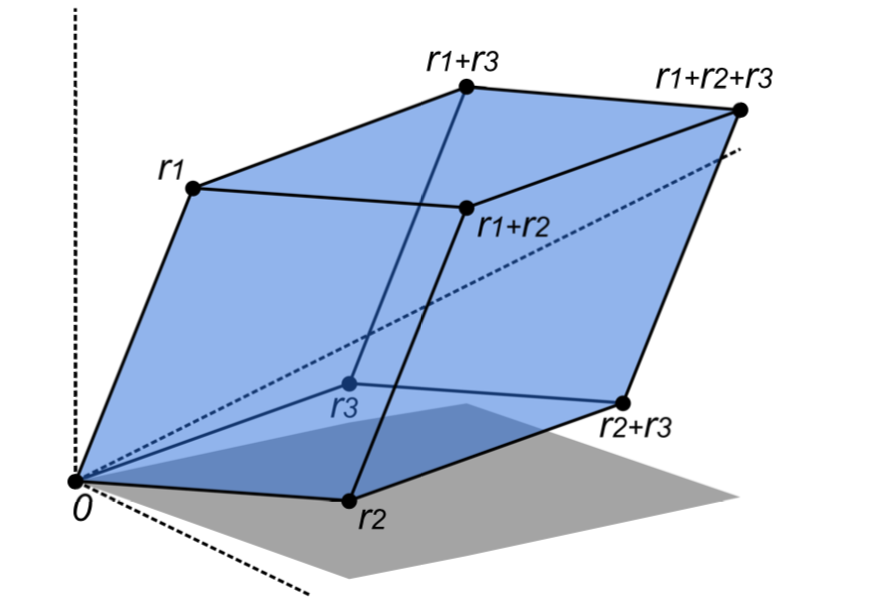
\includegraphics[width=6cm]{week4/F_1.png}
\caption{The parallelepiped $\mathcal{P}=\{y=\sum_{i=1}^3\alpha_i\bm a_i\mid \alpha_i\in[0,1]\}$, where $r_1,r_2,r_3$ are $\bm a_1,\bm a_2,\bm a_3$ on $\mathbb{R}^3$}
\end{figure}
\paragraph{The product of all the pivots $=(\pm 1)\x$the determinant}

For a 2 by 2 matrix $\bm A=\begin{bmatrix}
a&b\\c&d
\end{bmatrix}$, the pivots are $a$ and $d-(\frac{c}{a})b$. The product of pivots is the determinant:
\[
\begin{array}{lll}
\mbox{\emph{Product of pivots}}
&
a(d-\frac{c}{a}b)=ad-bc
&
\mbox{\emph{which is} $\det\bm A$}
\end{array}
\]
\paragraph{Compute determinants to find $\bm A^{-1}$ and $\bm A^{-1}\bm b$} (Cramer's Rule).

\subsubsection{The properties of the Determinant}
We don't intend to define the determinant directly by its formulas. It's better to start with its properties. These properties are simple, but they prepare for the formulas.
\begin{remark}
Brackets for the matrix, straight bars for its determinant. For example,
\[
\text{The determinant of }\begin{bmatrix}
a&b\\c&d
\end{bmatrix} \text{ is } \begin{vmatrix}
a&b\\c&d\end{vmatrix}=ad-bc
\]
The determinant is written in two ways, det $\bm A$ or $|\bm A|$.
\end{remark}

We will introduce three basic properties, then we will show how properties $1-3$ derive other properties.
\begin{enumerate}
\item
\emph{The determinant of the $\bm n$ by $\bm n$ identity matrix is 1.}
\begin{gather*}
\begin{vmatrix}1&0\\0&1\end{vmatrix}=1\qquad\text{and}\qquad\begin{vmatrix}
1&&\\&\ddots&\\&&1\end{vmatrix}=1.
\end{gather*}
\item
\emph{The determianant changes sign when two rows are exchanged.} (sign reversal)
\begin{gather*}
\text{Check:   }\begin{vmatrix}c&d\\a&b\end{vmatrix}=-\begin{vmatrix}a&b\\c&d\end{vmatrix}\qquad\text{(both sides equal $bc-ad$)}.
\end{gather*}
\item
\emph{The determinant is a linear function of each row separately.} (all other rows stay fixed).
\begin{gather*}
\text{\emph{multiply row 1 by any number $\bm t$}}\qquad\begin{vmatrix}ta&tb\\c&d\end{vmatrix}=t\begin{vmatrix}a&b\\c&d\end{vmatrix}
\end{gather*}
\begin{gather*}
\text{\emph{Add row 1 of $\bm A$ to row 1 of $\bm B$:}}\qquad\begin{vmatrix}a_1+a_2&b_1+b_2\\c&d\end{vmatrix}=\begin{vmatrix}a_1&b_1\\c&d\end{vmatrix}+\begin{vmatrix}a_2&b_2\\c&d\end{vmatrix}
\end{gather*}

Note that this rule \emph{deos not} mean $\det (\bm A+\bm B)=\det \bm A+\det\bm B$.

Note that this rule \emph{does not} mean $\det(t\bm A)=t\det(\bm A)$.

Actually, $\det(t\bm A)=t^n\det \bm A$. This is reasonable. Imagining that expanding a rectangle by 2, its area will increase by 4. Expand an $n-$dimensional box by $t$ and its volumn will increase by $t^n$.

Pay special attention to property $1\sim 3$. They completely determine the $\det\bm A$. We could stop here to find a formula for determinants. But before that we prefer to derive other properties that follow directly from the first three:
\item
\emph{If two rows of $\bm A$ are equal, then $\det\bm A=\bm0$.}
\begin{gather*}
\text{Check 2 by 2:   }\begin{vmatrix}a&b\\a&b\end{vmatrix}
=0.
\end{gather*}
Property 4 follows from Property 2.
\begin{proof}[Proofoutline.]
\textit{Exchange the two equal row.} The determinant $\bm D$ is supposed to change sign. But also the matrix is not changed, so we have $-\bm D=\bm D\implies\bm D=0$.
\end{proof}
\item
\emph{Adding a constant multiple of a row to another row doesn't change $\det\bm A$.}
\[
\begin{vmatrix}a+lc&b+ld\\c&d\end{vmatrix}=
\begin{vmatrix}a&b\\c&d\end{vmatrix}+\begin{vmatrix}lc&ld\\c&d\end{vmatrix}=\begin{vmatrix}a&b\\c&d\end{vmatrix}+l\begin{vmatrix}c&d\\c&d\end{vmatrix}=
\begin{vmatrix}a&b\\c&d\end{vmatrix}=\det\bm A
\]
\emph{Conclusion: }\textit{The determinant is not changed by the usual elimination step from $\bm A$ to $\bm U$}. Since every row exchange reverses the sign, we have $\det\bm A=\pm\det\bm U$.
\item
\emph{If $\bm A$ is triangular, then $\det\bm A=$ product of diagonal entries}.
\begin{gather*}
\text{\emph{Triangular}}\qquad\begin{vmatrix}a&b\\0&d\end{vmatrix}=ad\qquad\text{and also}\qquad\begin{vmatrix}a&0\\c&d\end{vmatrix}=ad
\end{gather*}
Suppose all diagonal entries of $\bm A$ are nonzero. We do Gaussian Elimination to convert $\bm A$ into diagonal matrix:
\[
\det\begin{bmatrix}
a_{11}&&&\bigzero\\&a_{22}&&\\&&\ddots&\\\bigzero&&&a_{nn}
\end{bmatrix}=a_{11}a_{22}\dots a_{nn}.
\]
Factor $a_{11}$ from the first row by property 3; then factor $a_{22}$ from the second row;$\dots\dots$. Finally the determinant is $a_{11}\x a_{22}\x a_{33}\dots\x a_{nn}\x\det\bm I=a_{11}\x a_{22}\x a_{33}\dots\x a_{nn}$.
\item 
$\det(\bm{AB})=\det(\bm A)\det(\bm B)$.
\begin{proof}\qquad\\
\begin{itemize}
\item
If $|\bm B|$ is zero, it's easy to verify that $\bm B$ is singular, then $\bm{AB}$ is singular. Thus $\det(\bm{AB})=0=\det(\bm A)\det(\bm B)$.
\item
Suppose $|\bm B|$ is not zero, and $\bm A,\bm B$ is $n\x n$ matrix. Consider the ratio $D(\bm A)=\frac{|\bm{AB}|}{|\bm B|}$. \textit{Check that this ratio has properties 1,2,3.} If so, $D(\bm A)$ has to be the determinant, say, $|\bm A|$. Thus we have $|\bm A|=\frac{|\bm{AB}|}{\bm B}$:\\\\
\emph{Property 1  }\textit{(Determinant of I)}\quad If $\bm A=\bm I$, then the ratio becomes $D(\bm A)=\frac{|\bm B|}{|\bm B|}=1.$\\\\
\emph{Property 2  }\textit{(Sign reversal)}\quad When two rows of $\bm A$ are exchanged, the same two rows of $\bm{AB}$ are also exchanged. Therefore $|\bm{AB}|$ changes sign and so does the ratio $\frac{|\bm{AB}|}{\bm B}$.\\\\
\emph{Property 3  }\textit{(Linearity)}\quad When row 1 of $\bm A$ is multiplied by $t$, so is row 1 of $\bm{AB}$. Thus the ratio is also increased by $t$. Thus we still have $|\bm A|=\frac{|\bm{AB}|}{\bm B}$.\\
If we Add row 1 of $\bm A_1$ to row 1 of $\bm A_2$. Then row 1 of $\bm A_1\bm B$ also adds to row 1 of $A_2B$. By property three, determinants add. After dividing by $|\bm B|$, the ratios add. Hence we still have $|\bm A|=\frac{|\bm{AB}|}{\bm B}$.\\\\
\textit{Conclusion: }The ratio $D(\bm A)$ has the same three properties that defines determinant, hence it equals $|\bm A|$. Hence we obtain the product rule $|\bm{AB}|=|\bm A||\bm B|$.\\
\end{itemize}
\end{proof}

Immediately here follows a corollary:
\begin{corollary}
\[\det(\bm A^{-1})=\frac{1}{\det(\bm A)}\]
\end{corollary}
\item
\emph{The transpose $\bm A\trans$ has the same determinant as $\bm A$.}
\begin{gather*}
\text{\emph{Transpose}}\qquad\begin{vmatrix}a&b\\c&d\end{vmatrix}=\begin{vmatrix}a&c\\b&d\end{vmatrix}\qquad\text{Both sides equal $ad-bc$}.
\end{gather*}
\begin{proof}
\begin{itemize}
\item
When $\bm A$ is singular, $\bm A\trans$ is also singular. Hence $|\bm A\trans|=|\bm A|=0$.
\item
Otherwise $\bm A$ has LU decomposition $\bm{PA}=\bm{LU}$. Transposing both siders gives $\bm A\trans\bm P\trans=\bm U\trans\bm L\trans$. By product rule we have
\[
\det\bm P\det\bm A=\det\bm L\det\bm U\qquad\text{and}\qquad\det\bm A\trans\det\bm P\trans=\det\bm U\trans\det\bm L\trans.
\]
\begin{itemize}
\item
Firstly, $\det\bm L=\det\bm L\trans=1$. (By property 6, they both have 1's on the diagonal).
\item
Secondly, $\det\bm U=\det\bm U\trans$. (By property 6, they have the same diagonal)
\item
Thirdly, $\det\bm P=\det\bm P\trans$. (Verify by yourself that $\bm P\trans\bm P=\bm I$. Hence $|\bm P\trans||\bm P|=1$. Since permutation matrix is obtained by exchanging rows of $\bm I$, the only possible value for determinant of permuation matrix is $\pm 1$. Hence $\bm P$ and $\bm P\trans$ must both equal to 1 or both equal to -1).
\end{itemize}
So $\bm{L,U,P}$ has the same determinants as $\bm L\trans,\bm U\trans,\bm P\trans$, Hence we have $\det\bm A=\det\bm A\trans$.
\end{itemize}
\end{proof}
\end{enumerate}













\section{Assignment Five}\index{Assignment_Five}
\begin{enumerate}
\item
Prove the following properties of \textit{similarity}:
\begin{enumerate}
\item
Any square matrix $\bm A$ is \textit{similar} to itself.
\item
If $\bm B$ is \textit{similar} to $\bm A$, then $\bm A$ is \textit{similar} to $\bm B$.
\item
If $\bm A$ is \textit{similar} to $\bm B$ and $\bm B$ is \textit{similar} to $\bm C$, then $\bm A$ is \textit{similar} to $\bm C$.
\end{enumerate}
\item
Consider the linear operator
\[
L\left(\begin{bmatrix}
x\\y
\end{bmatrix}\right)=\begin{bmatrix}
3x\\x-y
\end{bmatrix}
\]
on $\mathbb{R}^2$, use a \textit{similarity transformation} to find the \textit{matrix representation} with respect to the basis
\[
B=\left\{
\begin{bmatrix}
1\\2
\end{bmatrix},\begin{bmatrix}
2\\3
\end{bmatrix}
\right\}
\]
\item
Let $\mathbb{R}[x]$ be the vector space of all real polynomials in $x$. Determine whether the
following sets are subspaces of $\mathbb{R}[x]$. Justify your answer.
\begin{enumerate}
\item
All polynomials $f(x)$ of degree $\ge3$.
\item
All polynomials $f(x)$ satisfying $f(1)+2f(2)=1$.
\item
All polynomials $f(x)$ satisfying $f(x)=f(1-x)$.
\end{enumerate}
\item
Let $V=\{a+bx+cy+dx^2+exy+fy^2|a,b,c,d,e,f\in\mathbb{R}\}$, where $x,y$ are \textit{variables}. Then $V$ is just the set of all polynomials in $x$ and $y$ of degree two or less. One can show that
$V$ is a vector space in which the same way as we showed $\mathbb{P}_2$ is a vector space.\\
Now consider the function
\[
T:V\mapsto V\text{ by }T(f)=\frac{\partial f}{\partial x}-\frac{\partial f}{\partial y}
\]
where $f$ denotes  arbitrary vector in $V$.
\begin{enumerate}
\item
Prove that $T$ is a \textit{linear transformation}.
\item
Find bases for $kernel(T)$.
\end{enumerate}
\item
Let $S$ be the subspace of $C[a,b]$ spanned by $e^x$,$xe^x$ and $x^2e^x$. Let $D$ be the \textit{differentiation
operator} of $S$. 
Find the \textit{matrix representation} of $D$ with respect to $\{e^x,xe^x,x^2e^x\}$.
\item
Suppose all vectors $x$ in the unit square $0\le x_1\le 1,0\le x_2\le 1$ are transformed to $\bm{Ax}.$
($\bm A$ is 2 by 2)
\begin{enumerate}
\item
What's the shape of the \textit{transformed} region (all $\bm{Ax}$)?
\item
For which matrices $\bm A$ is that region a \textit{square}?
\end{enumerate}
\item
\begin{enumerate}
\item
Show the column space of $\bm A\bm A\trans$ and $\bm A$ are the same.
\item
Show the rank of $\bm A\trans\bm A,\bm A\bm A\trans,\bm A\trans,\bm A$ are the same.
\end{enumerate}
\end{enumerate}
%\include{week5/Lecture_1}
%\include{week5/Lecture_2}

\chapter{Week5}

\section{Tuesday}\index{week5_Tuesday_lecture}
\subsection{Formulas for Determinant}
We want to use the \emph{3 basic properties} to derive the formula for determinant:
\begin{enumerate}
\item
\emph{The determinant of the $\bm n$ by $\bm n$ identity matrix is 1.}
\begin{gather*}
\begin{vmatrix}1&0\\0&1\end{vmatrix}=1\qquad\text{and}\qquad\begin{vmatrix}
1&&\\&\ddots&\\&&1\end{vmatrix}=1.
\end{gather*}
\item
\emph{The determianant changes sign when two rows are exchanged.} (sign reversal)
\begin{gather*}
\text{Check:   }\begin{vmatrix}c&d\\a&b\end{vmatrix}=-\begin{vmatrix}a&b\\c&d\end{vmatrix}\qquad\text{(both sides equal $bc-ad$)}.
\end{gather*}
\item
\emph{The determinant is a linear function of each row separately.} (all other rows stay fixed).
\begin{gather*}
\text{\emph{multiply row 1 by any number $\bm t$}}\qquad\begin{vmatrix}ta&tb\\c&d\end{vmatrix}=t\begin{vmatrix}a&b\\c&d\end{vmatrix}
\end{gather*}
\begin{gather*}
\text{\emph{Add row 1 of $\bm A$ to row 1 of $\bm B$:}}\qquad\begin{vmatrix}a_1+a_2&b_1+b_2\\c&d\end{vmatrix}=\begin{vmatrix}a_1&b_1\\c&d\end{vmatrix}+\begin{vmatrix}a_2&b_2\\c&d\end{vmatrix}
\end{gather*}
\end{enumerate}
Although we derive the formula for $\det\bm A$ is $\det\bm A=\pm\prod_i\text{pivots}_{i}$ (product of pivots), it is not \emph{explicit}. We begin some example to show how to derive the explicit formula for determinant.
\begin{example}
To derive the formula for determinant, let's start with $n=2$.

Given $\bm A=\begin{bmatrix}
a&b\\c&d
\end{bmatrix}$, our goal is to get $\det(\bm A) = ad-bc$.

We can break each row into two simpler rows:
\[
\begin{vmatrix}
a&b
\end{vmatrix}=\begin{vmatrix}
a&0
\end{vmatrix}+\begin{vmatrix}
0&b
\end{vmatrix}\qquad\text{and}\qquad
\begin{vmatrix}
c&d
\end{vmatrix}=\begin{vmatrix}
c&0
\end{vmatrix}+\begin{vmatrix}
0&d
\end{vmatrix}
\]
Now apply property 3, first in row 1(with row 2 fixed) and then in row 2(with row 1 fixed):
\[
\begin{aligned}
\begin{vmatrix}
a&b\\c&d
\end{vmatrix}&=\begin{vmatrix}
a&0\\c&d
\end{vmatrix}+\begin{vmatrix}
0&b\\c&d
\end{vmatrix}\\&=\begin{vmatrix}
a&0\\c&0
\end{vmatrix}+\begin{vmatrix}
a&0\\0&d
\end{vmatrix}+\begin{vmatrix}
0&b\\c&0
\end{vmatrix}+\begin{vmatrix}
0&b\\0&d
\end{vmatrix}
\end{aligned}
\]
The last line has $2^2=4$ determinants. The first and fourth are zero since their rows are \emph{dep.} (one row is a multiple of the other row.) We left two terms to compute:
\[
\begin{vmatrix}
a&0\\0&d
\end{vmatrix}+\begin{vmatrix}
0&b\\c&0
\end{vmatrix}=ad\begin{vmatrix}
1&0\\0&1
\end{vmatrix}+bc\begin{vmatrix}
0&1\\1&0
\end{vmatrix}=ad-bc
\]
The permutation matrices $\begin{bmatrix}
1&0\\0&1
\end{bmatrix}$ and $\begin{bmatrix}
0&1\\1&0
\end{bmatrix}$ have determinant $+1$ or $-1$.
\end{example}
\begin{example}
Now we try $n=3$. Each row splits into 3 simpler rows such as $\begin{bmatrix}
a_{11}&0&0
\end{bmatrix}$. Hence $\det\bm A$ will split into $3^3=27$ simple determinants. For simple determinant, if one column has two nonzero entries, (For example, $\begin{bmatrix}
a_{11}&0&0\\a_{21}&0&0\\0&0&a_{33}
\end{bmatrix}$), then its determinant will be zero.\\
Hence we only need to foucus on the matrix that \emph{the nonzero terms come from defferent columns}:
\[
\begin{aligned}
\begin{vmatrix}
a_{11}&a_{12}&a_{13}\\a_{21}&a_{22}&a_{23}\\a_{31}&a_{32}&a_{33}
\end{vmatrix}
&=
\begin{vmatrix}
a_{11}&&\\&a_{22}&\\&&a_{33}
\end{vmatrix}
+
\begin{vmatrix}
&a_{12}&\\&&a_{23}\\a_{31}&&
\end{vmatrix}
+
\begin{vmatrix}
&&a_{13}\\a_{21}&&\\&a_{32}&
\end{vmatrix}\\&+
\begin{vmatrix}
a_{11}&&\\&&a_{23}\\&a_{32}&
\end{vmatrix}
+
\begin{vmatrix}
&a_{12}&\\a_{21}&&\\&&a_{33}
\end{vmatrix}
+
\begin{vmatrix}
&&a_{13}\\&a_{22}&\\a_{31}&&
\end{vmatrix}
\end{aligned}
\]
There are $3!=6$ ways to permutate the three columns, so there leaves six determinants. The six permutations of $(1,2,3)$ is given by:
\[
\mbox{{\emph{Column numbers}}} = (1,2,3),(2,3,1),(3,1,2),(1,3,2),(2,1,3),(3,2,1).
\]
The last three are \textit{odd permutations} (One exchange from identity permutation $(1,2,3)$.) The first three are \textit{even permutations}. (zero or two exchange from identity permutation $(1,2,3)$.) When the column number is $(\alpha,\beta,\omega)$, we get the entries $a_{1\alpha},a_{2\beta},a_{3\omega}$.  The permutation $(\alpha,\beta,\omega)$ comes with a plus or minus sign. If you don't understand, look at example below:
\[
\begin{aligned}
\det\bm A&=
a_{11}a_{22}a_{33}\begin{vmatrix}
1&&\\&1&\\&&1
\end{vmatrix}
+
a_{12}a_{23}a_{31}\begin{vmatrix}
&1&\\&&1\\1&&
\end{vmatrix}
+
a_{13}a_{21}a_{32}\begin{vmatrix}
&&1\\1&&\\&1&
\end{vmatrix}\\&+
a_{11}a_{23}a_{32}\begin{vmatrix}
1&&\\&&1\\&1&
\end{vmatrix}
+
a_{12}a_{21}a_{33}\begin{vmatrix}
&1&\\1&&\\&&1
\end{vmatrix}
+
a_{13}a_{22}a_{31}\begin{vmatrix}
&&1\\&1&\\1&&
\end{vmatrix}
\end{aligned}
\]
The first three (even) permutation matrices have $\det\bm P=+1$, the last three (odd) permutation matrices have $\det\bm P=-1$. Hence we have:
\[
\begin{aligned}
\det\bm A&=a_{11}a_{22}a_{33}+
a_{12}a_{23}a_{31}+
a_{13}a_{21}a_{32}-
a_{11}a_{23}a_{32}-
a_{12}a_{21}a_{33}-
a_{13}a_{22}a_{31}\\
&=a_{11}(a_{22}a_{33} - a_{23}a_{32})+a_{12}(a_{23}a_{31}-a_{21}a_{33})+a_{13}(a_{21}a_{32}-a_{22}a_{31})
\end{aligned}
\]
\end{example}
\subsubsection{$n$ by $n$ formula of determinant}
Now we can see $n$ by $n$ formula. There are $n!$ permutations of columns, so we have $n!$ terms for determinant. 

Assuming $(\alpha,\beta,\dots,\omega)$ is the permutation of $(1,2,\dots,n)$. The coorsponding term is $a_{1\alpha}a_{2\beta}\dots a_{n\omega}\det\bm P$, where $\bm P$ is the permutation matrix with column number $\alpha,\beta,\dots,\omega$.

The complete determinant of $\bm A$ is the sum of these $n!$ simple determinants. $a_{1\alpha}a_{2\beta}\dots a_{n\omega}$ is obtained by choosing \emph{one entry from every row and every column:}
\begin{definition}[Big formula for determinant]
\[
\begin{aligned}
\det\bm A&=\text{sum of all $n!$ column permutations}\\
&=\sum(\det\bm P)a_{1\alpha}a_{2\beta}\dots a_{n\omega}=\text{\emph{BIG FORMULA}}
\end{aligned}
\]
where $\bm P$ is permutation matrix with column number $(\alpha,\beta,\dots,\omega)$. And $\{\alpha,\beta,\dots,\omega\}$ is a permutation of $\{1,2,\dots,n\}$.
\end{definition}
\begin{remark}
\paragraph{Complexity Analysis}
However, if we want to use big formula to compute matrix, we need to do $n!(n-1)$ multiplications. If we use formula $\det\bm A=\pm\prod pivots$, we only need to do $O(n^3)$ multiplications. Hence the letter one is more efficient.
\end{remark}
\subsubsection{Verify property}
We can also use the big formula to verify property 1 to property 3:
\begin{itemize}
\item $\det\bm I=1$:\\
Only when $(\alpha,\beta,\dots,\omega)$=$(1,2,\dots,n)$, there is no zero entries for $a_{1\alpha}a_{2\beta}\dots a_{n\omega}$. Hence $\det\bm A=a_{11}a_{22}\dots a_{nn}=1$.
\item \emph{sign reversal}:\\
If two rows are interchanged, then all determinant of permutation matrix will change its sign, hence the value for determinant $\bm A$ is opposite.
\item \emph{The determinant is a linear function of each row separately}.\\
\emph{If we separate out the fator $a_{11},a_{12},\dots,a_{1\alpha}$ that comes from the first row}, this property is easy to check. For 3 by 3 matrix, separate the usual 6 terms of the determinant into 3 pairs:
\[
\det\bm A=a_{11}(a_{22}a_{33}-a_{23}a_{32})+a_{12}(a_{23}a_{31}-a_{21}a_{33})+a_{13}(a_{21}a_{32}-a_{22}a_{31}).
\]
Those three quantities in parentheses are called \emph{cofactors}. They are $2\times 2$ determinant coming from matrices in row 2 and 3. The first row contributes the factors $a_{11},a_{12},a_{13}$. The lower rows contribute the cofactors $(a_{22}a_{33}-a_{23}a_{32}),(a_{23}a_{31}-a_{21}a_{33}),(a_{21}a_{32}-a_{22}a_{31})$. Certainly $\det\bm A$ depends \emph{linearly} on $a_{11},a_{12},a_{13}$, which is property 3.
\end{itemize}
\subsection{Determinant by Cofactors}
We could write the determinant in this form:
\[
\begin{vmatrix}
a_{11}&a_{12}&a_{13}\\a_{21}&a_{22}&a_{23}\\a_{31}&a_{32}&a_{33}
\end{vmatrix}=
\begin{vmatrix}
a_{11}&&\\&a_{22}&a_{23}\\&a_{32}&a_{33}
\end{vmatrix}+
\begin{vmatrix}
&a_{12}&\\a_{21}&&a_{23}\\a_{31}&&a_{33}
\end{vmatrix}+
\begin{vmatrix}
&&a_{13}\\a_{21}&a_{22}&\\a_{31}&a_{32}&
\end{vmatrix}.
\]
If we define $\bm A_{1j}$ to be \emph{the submatrix obtained by removing row 1 and column j}, We could compute $\det\bm A$ in this way:
\begin{gather*}
\text{The cofactors along row 1 are } C_{1j}=(-1)^{1+j}\det\bm A_{1j}\quad j=1,2,\dots,n.\\
\text{\emph{The cofactor expansion is }} \det\bm A=a_{11}C_{11}+a_{12}C_{12}+\dots+a_{1n}C_{1n}.
\end{gather*}
More generally, we can cross row $i$ to get the determinant:
\begin{definition}[Determinant]
The determinant is the \emph{dot product} of any row $i$ of $\bm A$ with its cofactors using other rows:
\[
\text{\emph{Cofactor Formula}}\qquad\det\bm A=
a_{i1}C_{i1}+a_{i2}C_{i2}+\dots+a_{in}C_{in}.
\]
Each cofactor $C_{ij}$ is defined as:
\[
\text{\emph{Cofactor}}\qquad C_{ij}=(-1)^{i+j}\det\bm A_{ij}
\]
where $A_{ij}$ is the submatrix obtained by removing row $i$ and column $j$.
\end{definition}

\paragraph{Cofactors down a column} Since we have $\det\bm A=\det\bm A\trans$, we can expand the determinant in cofactors \textit{down a column} instead of across a row. Down column $j$ the entries are $a_{1j}$ to $a_{nj}$, the cofactors are $C_{1j}$ to $C_{nj}$. The determinant is given by:
\[
\begin{array}{ll}
\mbox{\emph{Cofactors down column $j$:}}
&
\det\bm A=a_{1j}C_{1j}+a_{2j}C_{2j}+\dots+a_{nj}C_{nj}.
\end{array}
\]
\subsection{Determinant Applications}
\subsubsection{Inverse}
It's easy to check that the inverse of 2 by 2 matrix $\bm A$ is 
\[
\begin{bmatrix}
a&b\\c&d
\end{bmatrix}^{-1}=\frac{1}{ad-bc}\begin{bmatrix}
d&-b\\-c&a
\end{bmatrix}=\frac{1}{\det\bm A}\begin{bmatrix}
d&-b\\-c&a
\end{bmatrix}.
\]
We could use determinant to compute inverse! Before that let's define \emph{cofactor matrix}:
\begin{definition}[cofactor matrix]
The cofactor matrix of $n\times n$ matrix $\bm A$ is given by:
\[
\bm C=\begin{bmatrix}
C_{ij}
\end{bmatrix}_{1\le i,j\le n}
\]
where $C_{ij}$ is the cofactor of $\bm A$.
\end{definition}
Then we try to derive the inverse of matrix $\bm A$. 
\begin{quotation}
For $n\times n$ matrix $\bm A$, the product of $\bm A$ and the \emph{transpose} of \textit{cofactor matrix} is given by:
\begin{equation}\label{11.1}
\bm A\bm C\trans=\begin{bmatrix}
a_{11}&\dots&a_{1n}\\\vdots&\ddots&\vdots\\a_{n1}&\dots&a_{nn}
\end{bmatrix}\begin{bmatrix}
C_{11}&\dots&C_{n1}\\\vdots&\ddots&\vdots\\C_{1n}&\dots&C_{nn}
\end{bmatrix}=\begin{bmatrix}
\det\bm A&&\\&\det\bm A&\\&&\det\bm A
\end{bmatrix}
\end{equation}
\end{quotation}
\emph{Proofoutline:} 
\begin{itemize}
\item
Row 1 of $\bm A$ times the column 1 of $\bm C\trans$ yields the first $\det\bm A$ on the right:
\[
a_{11}C_{11}+a_{12}C_{12}+\dots+a_{1n}C_{1n}=\det\bm A
\]
Similarly, row $j$ of $\bm A$ times column $j$ of $\bm C\trans$ yields the determinant.
\item
\textit{How to explain the zeros off the main diagonal in equation (\ref{11.1})?} Rows of $\bm A$ are multiplying $\bm C\trans$ from \emph{different} columns. Why is the answer zero? For example, the (2,1)th entry of the result is given by
\begin{equation}
\begin{aligned}
\text{\emph{Row 2 of $\bm A$}}\\
\text{\emph{Row 1 of $\bm C$}}
\end{aligned}
\qquad\qquad
a_{21}C_{11}+a_{22}C_{12}+\dots+a_{2n}C_{1n}=0.\label{Eq:6:2}
\end{equation}

\textit{Explaination for Eq.(\ref{Eq:6:2}): }
If the second row of $\bm A$ is copied into its first row, we define this new matrix as $\bm A^{*}$. Thus the determinant of $\bm A^{*}$ is given by:
\[
\begin{vmatrix}
a_{21}&a_{22}&\dots&a_{2n}\\
a_{21}&a_{22}&\dots&a_{2n}\\
a_{31}&a_{32}&\dots&a_{3n}\\
\vdots&\vdots&\ddots&\vdots\\
a_{n1}&a_{n2}&\dots&a_{nn}
\end{vmatrix}
=
\begin{vmatrix}
a_{21}&&&\\
&a_{22}&\dots&a_{2n}\\
&a_{32}&\dots&a_{3n}\\
&\vdots&\ddots&\vdots\\
&a_{n2}&\dots&a_{nn}
\end{vmatrix}
+
\begin{vmatrix}
&a_{22}&&\\
a_{21}&&\dots&a_{2n}\\
a_{31}&&\dots&a_{3n}\\
\vdots&&\ddots&\vdots\\
a_{n1}&&\dots&a_{nn}
\end{vmatrix}
+\dots+
\begin{vmatrix}
&&&a_{2n}\\
a_{21}&a_{22}&a_{2(n-1)}&\\
a_{31}&a_{32}&a_{3(n-1)}&\\
\vdots&\vdots&\vdots&\\
a_{n1}&a_{n2}&a_{n(n-1)}&
\end{vmatrix}
\]
Or equivalently, we have
\[\det\bm A^{*}=
\begin{vmatrix}
a_{21}&a_{22}&\dots&a_{2n}\\
a_{21}&a_{22}&\dots&a_{2n}\\
a_{31}&a_{32}&\dots&a_{3n}\\
\vdots&\vdots&\ddots&\vdots\\
a_{n1}&a_{n2}&\dots&a_{nn}
\end{vmatrix}
=a_{21}C_{11}+a_{22}C_{12}+\dots+a_{2n}C_{1n}
\]
Since $\bm A^{*}$ has two equal rows, the determinant must be zero. Hence $a_{21}C_{11}+a_{22}C_{12}+\dots+a_{2n}C_{1n}=0.$

Similarly, \emph{all entries off the main diagonal in Eq.(\ref{11.1}) are zero.}
\end{itemize}	
Thus the equation $(\ref{11.1})$ is correct:
\[
\bm A\bm C\trans=\begin{bmatrix}
\det\bm A&&\\&\det\bm A&\\&&\det\bm A
\end{bmatrix}=\det(\bm A)\bm I
\implies
\bm A^{-1}=\frac{1}{\det\bm A}\bm C\trans.
\]
Hence we could compute the inverse by computing many determinants of submatrix:
\begin{definition}[Inverse]
\emph{The $(\bm i,\bm j)$th entry of $\bm A^{-1}$ is the cofactor $C_{ji}$ (not $C_{ji}$) divided by $\det\bm A$: }
\[
\mbox{\emph{Formula for $\bm A^{-1}$}}\qquad\qquad
(\bm A^{-1})_{ij}=\frac{C_{ji}}{\det\bm A}\qquad\text{and}\qquad\bm A^{-1}=\frac{\bm C\trans}{\det\bm A}.
\]
\end{definition}
\subsubsection{Cramer's Rule}
\paragraph{Cramer's Rule solves $\bm{Ax}=\bm b$}

Assume $\bm A$ is a $n\times n$ matrix that is \emph{nonsingular}. Then we can use determinant to solve this system:

Let's start with $n=3$. We could multiply $\bm A$ with a new matrix $\bm C_1$ to get $\bm B_1$:
\[
\begin{array}{ll}
\mbox{\emph{Key idea:}}
&
\bm A\bm C_1
=
\begin{bmatrix}
a_{11}&a_{12}&a_{13}\\a_{21}&a_{22}&a_{23}\\a_{31}&a_{32}&a_{33}
\end{bmatrix}\begin{bmatrix}
x_1&0&0\\x_2&1&0\\x_3&0&1
\end{bmatrix}=\begin{bmatrix}
b_1&a_{12}&a_{13}\\b_2&a_{22}&a_{23}\\b_3&a_{32}&a_{33}
\end{bmatrix}=\bm B_1
\end{array}
\]
Taking determinants both sides, then we have
\[
\det(\bm A\bm C_1)=\det(\bm A)\det(\bm C_1)=\det(\bm A)(x_1)=\det\bm B_1\implies
x_1=\frac{\det\bm B_1}{\det\bm A_1}.
\]
The matrix $\bm B_1$ is essentaily obtained by replacing the first column of $\bm A$ by the vector $\bm b$.

Similarly, we could get all $x_j$ in this way. $(i=1,\dots,n)$.
\begin{definition}[Cramer's Rule]
If $\det\bm A$ is not zero, $\bm{Ax}=\bm b$ could be solved by determinants:
\[
x_1=\frac{\det\bm B_1}{\det\bm A}\qquad
x_2=\frac{\det\bm B_2}{\det\bm A}\qquad
\dots\dots\qquad
x_n=\frac{\det\bm B_n}{\det\bm A}
\]
The matrix $\bm B_j$ has the $j$th column of $\bm A$ replaced by the vector $\bm b$. In other words,
\[
\begin{array}{ll}
\bm B_{j}=\begin{bmatrix}
a_{11}&\dots&b_1&\dots&a_{1n}\\
a_{21}&\dots&b_2&\dots&a_{2n}\\
\vdots&\ddots&\vdots&\ddots&\vdots\\
a_{n1}&\dots&b_n&\dots&a_{nn}\\
\end{bmatrix}\
&
j=1,\dots,n.
\end{array}
\]
\end{definition}
\subsection{Orthogonality}
\begin{definition}[Orthogonal vectors]
Two vectors $\bm x,\bm y\in\mathbb{R}^{n}$ are orthogonal when their inner product is zero:
\[
\inp{\bm x}{\bm y}=\sum_{i=1}^{n}x_{i}y_{i}=0.
\]
\end{definition}
\begin{remark}
Note that the inner product of two \emph{vectors} satisfies the \textit{commutative rule}. In other words, $\inp{\bm x}{\bm y}=\inp{\bm y}{\bm x}$ for vectors $\bm x$ and $\bm y$. The inner product defined for matrices may not satisfy the \textit{commutative rule}. Generally, if the result of inner product is a scalar, then inner product satisfies commutative rule.
\end{remark}
An important case is the inner product of a vector with \textit{itself}. The inner product $\inp{\bm x}{\bm x}$ gives the \textit{length of $\bm v$ squared}:
\begin{definition}[length/norm]
The \emph{length}(\emph{norm}) $\|\bm x\|$ of a vector $\bm x\in\mathbb{R}^n$ is the square root of $\inp{\bm x}{\bm x}$:
\[
\mbox{\emph{length}}=\|\bm x\|=\sqrt{\inp{\bm x}{\bm x}}=\sqrt{x_1^2+\dots+x_n^2}.
\]
\end{definition}
\subsubsection{Function space}
We can talk about inner product between functions under the function space. For example, if we define $V=\{f(t)\mid \int_{0}^{1}f^2(t)dt<\infty\}$, then we can define inner product and norm under $V$:
\begin{definition}[Inner product; norm]
The \emph{inner product} and the \emph{norm} of $f(x),g(x)$ under the function space $V=\{f(t)\mid \int_{0}^{1}f^2(t)dt<\infty\}$, are defined as:
\[
\inp{f}{g}=\int_{0}^{1}f(x)g(x)dx
\qquad\mbox{and}\qquad
\|f\|^2=\sqrt{\int_{0}^{1}f^2(x)dx}
\]
\end{definition}
Moreover, when $\inp{f}{g}=0$, we say two functions are \emph{orthogonal} and denote it as $f\perp g$.
\subsubsection{Cauchy-Schwarz Inequality}
In $\mathbb{R}^2$, suppose $\bm x=\begin{pmatrix}
x_1\\x_2
\end{pmatrix},\bm y=\begin{pmatrix}
y_1\\y_2
\end{pmatrix}$, then we set:
\[
\begin{array}{ll}
\left\{
\begin{aligned}
x_1=\|\bm x\|\cos\theta\\
x_2=\|\bm x\|\sin\theta
\end{aligned}
\right.
&
\left\{
\begin{aligned}
y_1=\|\bm y\|\cos\varphi\\
y_2=\|\bm y\|\sin\varphi
\end{aligned}
\right.
\end{array}
\]
The inner product of $\bm x$ and $\bm y$ is given by:
\[
\begin{aligned}
<\bm x,\bm y>=\bm x\trans\bm y&=x_1x_2+y_1y_2\\
											 &=\|\bm x\|\|\bm y\|(\cos\theta\cos\varphi+\sin\theta\sin\varphi)\\
											 &=\|\bm x\|\|\bm y\|\cos(\theta-\varphi)
\end{aligned}
\]
Since $|\cos(\theta-\varphi)|$ never exceeds 1, the cosine formula gives a great inequality:
\begin{theorem}[Cauchy Schwarz Inequality]
\[
\inp{\bm x}{\bm y}\le\|\bm x\|\|\bm y\|
\]
holds for two vectors $\bm x$ and $\bm y$.
\end{theorem}
\begin{proof}
Firstly, we want to find optimizer $t^{*}$ such that 
\[
\min\|\bm x-t\bm y\|^2=\|\bm x-t^{*}\bm y\|^2.
\]
Note that
\[\begin{aligned}
\|\bm x-t\bm y\|^2&=\inp{\bm x-t\bm y}{\bm x-t\bm y}=\inp{\bm x}{\bm x}+\inp{-t\bm y}{\bm x}+\inp{\bm x}{-t\bm y}+\inp{-t\bm y}{-t\bm y}\\
&=\|\bm x\|^2-t\inp{\bm y}{\bm x}-t\inp{\bm x}{\bm y}+t^2\|\bm y\|^2\\
&=\|\bm x\|^2-2t\inp{\bm x}{\bm y}+t^2\|\bm y\|^2
\end{aligned}
\]
Hence the minimizer $t*$ must satisfy
\[
\Delta=0\implies
t^{*}=\frac{\inp{\bm x}{\bm y}}{\|\bm y\|^2}
\]
Hence we have 
\[\begin{aligned}
\|\bm x-t\bm y\|^2_{\min}=\|\bm x-t^*\bm y\|^2&=
\|\bm x\|^2-\frac{\inp{\bm x}{\bm y}^2}{\|\bm y\|^2}\\
&=\frac{\|\bm x\|^2\|\bm y\|^2-\inp{\bm x}{\bm y}^2}{\|\bm y\|^2}\ge 0\\
\qquad\qquad\implies
\|\bm x\|^2\|\bm y\|^2\ge\inp{\bm x}{\bm y}^2
\end{aligned}
\]
Or equivalently,
\[
|\inp{\bm x}{\bm y}|\le\|\bm x\|\|\bm y\|.
\]
\end{proof}
\begin{remark}
\paragraph{Cauchy-Schwarz inequality also holds for functions}
If we consider functions $f,g$ as vectors, then
\[
\left[
\int_0^1f(t)g(t)dt
\right]\le
\int_0^1f^2dt\int_0^1g^2dt
\]
\paragraph{The normalization of inner product is bounded by 1}
Since $|\inp{\bm x}{\bm y}|\le\|\bm x\|\|\bm y\|$, we have 
\[
-1\le\frac{\inp{\bm x}{\bm y}}{\|\bm x\|\|\bm y\|}\le 1
\]
If we define $\frac{\inp{\bm x}{\bm y}}{\|\bm x\|\|\bm y\|}:=\cos\theta$, then $\inp{\bm x}{\bm y}=\|\bm x\|\|\bm y\|\cos\theta$, the angle $\theta$ is said to be the intersection angle between $\bm x$ and $\bm y$.
\end{remark}
Cauchy-Schwarz equality holds for \emph{Hilbert space}, which will be discussed in other courses.

\subsubsection{Orthogonal for space}
After defining inner product, we can discuss the orthogonality for space:
\begin{definition}[Orthogonal subspaces]
Two subspaces $\bm U$ and $\bm V$ of a vector space are \emph{orthogonal} if every vector $\bm u$ in $\bm U$ is \textit{perpendicular} to every vector $\bm v$ in $\bm V$:
\[
\begin{array}{ll}
\mbox{\emph{Orthogonal subspaces}}
&
\inp{\bm u}{\bm v}=0\mbox{ for all $\bm u$ in $\bm U$ and all $\bm v$ in $\bm V$.}
\end{array}
\]
\end{definition}

\section{Thursday}\index{week5_Thursday_lecture}
\subsection{Orthogonality}
Recall that two vectors are orthogonal if their inner product is zero:
\[
\bm u\perp\bm v
\Longleftrightarrow
\inp{\bm u}{\bm v}=0
\]

Orthogonality among vectors has an important property:
\begin{proposition}
If \emph{nonzero} vectors $v_1,\dots,v_k$ are mutually orthogonal, i.e., $v_i\perp v_j$ for any $i\ne j$, then $\{v_1,\dots,v_k\}$ must be ind.
\end{proposition}
\begin{proof}
It suffices to show that 
\[
\alpha_1v_1+\dots+\alpha_kv_k=\bm 0 \implies
\alpha_i=0\text{ for any $i\in\{1,2,\dots,k\}$.}
\]
\begin{itemize}
\item
We do inner product to show $\alpha_1$ must be zero:
\[
\begin{aligned}
\inp{v_1}{\alpha_1v_1+\dots+\alpha_kv_k}
&=\inp{v_1}{\bm 0}=0\\
&=\alpha_1\inp{v_1}{v_1}+\alpha_2\inp{v_1}{v_2}+\dots+\alpha_k\inp{v_1}{v_k}\\
&=\alpha_1\inp{v_1}{v_1}=\alpha_1\|v_1\|_2^2\\
&=0
\end{aligned}
\]
Since $v_1\ne \bm 0$, we have $\alpha_1=0$.
\item
Similarly, we have $\alpha_i=0$ for $i=1,\dots,k$.
\end{itemize}
\end{proof}
Now we can also talk about orthogonality among spaces:
\begin{definition}[Subspace Orthogonality]
Two subspaces $\bm U$ and $\bm V$ of a vector space are \emph{orthogonal} if every vector $\bm u$ in $\bm U$ is \textit{perpendicular} to every vector $\bm v$ in $\bm V$:
\[
\begin{array}{lll}
\mbox{\emph{Orthogonal subspaces}}
&
\bm u\perp\bm v,
&
\forall\bm u\in\bm U,\bm v\in\bm V.
\end{array}
\]
\end{definition}
\begin{example}
Two walls look \textit{perpendicular} but they are not orthogonal subspaces! The meeting line is in both $\bm U$ and $\bm V$-and this line is not perpendicular to itself. Hence, two planes (both with dimension $2$ in $\mathbb{R}^{3}$) cannot be orthogonal subspaces.

\begin{figure}[H]
\centering
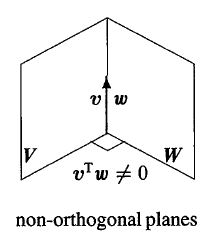
\includegraphics{week5/orthogonality}
\caption{Orthogonality is impossible when $\dim\bm U+\dim\bm V>\dim(\bm U\cup\bm V)$}
\end{figure}
\end{example}
\begin{remark}
When a vector is in two orthogonal subspaces, it \textit{must} be zero. It is \emph{perpendicular} to
itself. 
\\The reason is clear: this vector $\bm u\in\bm U$ and $\bm u\in\bm V$, so $\inp{\bm u}{\bm u}=0$. It has to be zero vector.
\end{remark}
If two subspaces are perpendicular, their basis must be ind.
\begin{theorem}
Assume $\{u_1,\dots,u_k\}$ is the basis for $\bm U$, $\{v_1,\dots,v_l\}$ is the basis for $\bm V.$ If $\bm U\perp\bm V$ ($u_i\perp v_j$ for $\forall i,j$), then $u_1,u_2,\dots,u_k,v_1,v_2,\dots,v_l$ must be ind.
\end{theorem}
\begin{proof}
Suppose there exists $\{\alpha_1,\dots,\alpha_k\}$ and $\{\beta_1,\dots,\beta_l\}$ such that
\[
\alpha_1u_1+\dots+\alpha_ku_k+\beta_1v_1+\dots+\beta_lv_l=\bm 0
\]
then equivalently,
\[
\alpha_1u_1+\dots+\alpha_ku_k=-(\beta_1v_1+\dots+\beta_lv_l).
\]
Then we set $\bm w=\alpha_1u_1+\dots+\alpha_ku_k$, obviously, $\bm w\in\bm U$ and $\bm w\in\bm V$.

 Hence it must be zero (This is due to remark above). Thus we have
\begin{gather*}
\alpha_1u_1+\dots+\alpha_ku_k=\bm 0\\
\beta_1v_1+\dots+\beta_lv_l=\bm 0.
\end{gather*}
Due to the independence, we have $\alpha_i=0$ and $\beta_j=0$ for $\forall i,j$. 
\end{proof}
\begin{corollary}
For subspaces $\bm U$ and $\bm V$, we obtain
\[
\dim(\bm U\cup\bm V)\le \dim(\bm U) + \dim(\bm V).
\]
\end{corollary}
For subspaces $\bm U$ and $\bm V\in\mathbb{R}^{n}$, if $\mathbb{R}^{n}=\bm U\cup\bm V$, and moreover, $n=\dim(\bm U)+\dim(\bm V)$, then we say $\bm V$ is the \emph{orthogonal complement} of $\bm U$.
\begin{definition}[orthogonal complement]
For subspaces $\bm U$ and $\bm V\in\mathbb{R}^{n}$, if $\dim(\bm U)+\dim(\bm V)=n$ and $\bm U\perp\bm V$, then we say $\bm V$ is the \emph{orthogonal complement} of $\bm U$. We denote $\bm V$ as $\bm U^{\perp}$.

Moreover, $\bm V=\bm U^{\perp}$ iff $\bm V^{\perp}=\bm U$.
\end{definition}
\begin{example}
Suppose $\bm U\cup\bm V=\mathbb{R}^{3}$, $\bm U=\Span\{\bm e_1,\bm e_2\}$. If $\bm V$ is the orthogonal complement of $\bm U$, then $\bm V=\Span\{\bm e_3\}$.
\end{example}

Next we study the relationship between the null space and the row space in $\mathbb{R}^n$.
\begin{theorem}[Fundamental theorem for linear alegbra, part 2] Given $\bm A\in\mathbb{R}^{m\times n}$,

\emph{$N(\bm A)$ is the orthogonal complement of the row space of $\bm A$, $\mathcal{C}(\bm A\trans)$ (in $\mathbb{R}^{n}$).}

\emph{$N(\bm A\trans)$ is the orthogonal complement of the column space $\mathcal{C}(\bm A)$ (in $\mathbb{R}^{m}$).}
\end{theorem}
\begin{proof}
\begin{itemize}
\item
Firstly, we show $\dim(N(\bm A))+\dim(\mathcal{C}(\bm A\trans))=n$:

We know that $\dim(N(\bm A))=n-r$ and $\dim(\mathcal{C}(\bm A\trans)) = r$, where $r=\rank(\bm A)$.

Hence $\dim(N(\bm A))+\dim(\mathcal{C}(\bm A\trans))=n$.
\item
Then we show $N(\bm A)\perp \mathcal{C}(\bm A\trans)$:

For any $x\in N(\bm A)$, if we set $\bm A=\begin{bmatrix}
a_1\trans\\a_2\trans\\\vdots\\a_m\trans
\end{bmatrix}$, then we obtain:
\[
\bm{Ax}=\begin{bmatrix}
a_1\trans\\a_2\trans\\\vdots\\a_m\trans
\end{bmatrix}\begin{bmatrix}
\bm x
\end{bmatrix}=\begin{bmatrix}
0\\0\\\vdots\\0
\end{bmatrix}
\]
Hence \textit{every row has a zero product with} $\bm x$, i.e., $\inp{a_i}{\bm x}=0$ for $\forall i\in\{1,2,\dots,m\}$.

For any $y=\sum_{i=1}^m\alpha_ia_i\in \mathcal{C}	(\bm A\trans)$, we obtain:
\[
\begin{aligned}
\inp{\bm x}{y}&=\inp{y}{\bm x}=\inp{\sum_{i=1}^m\alpha_ia_i}{\bm x}\\
&=\sum_{i=1}^{m}\alpha_i\inp{a_i}{\bm x}=0.
\end{aligned}
\]
Hence $\bm x\perp y$ for $\forall \bm x\in N(\bm A)$ and $y\in \mathcal{C}(\bm A\trans)$.\\
\end{itemize}
Hence $N(\bm A)^{\perp}=\mathcal{C}(\bm A\trans)$. Similarly, we have $N(\bm A\trans)^{\perp}=\mathcal{C}(\bm A)$. 
\end{proof}

\begin{corollary}
$\bm{Ax}=\bm b$ is solvable if and only if $\bm y\trans\bm A=\bm 0$ implies $\bm y\trans\bm b$=0.
\end{corollary}
\begin{proof} The following statements are equivalent:
\begin{itemize}
\item
$\bm{Ax}=\bm b$ is solvable.
\item
$\bm b\in \mathcal{C}(\bm A)$.
\item
$\bm b\in N(\bm A\trans)^{\perp}$
\item
$\bm y\trans\bm b=0$ for $\forall y\in N(\bm A\trans)$
\item
Given $\bm y\trans\bm A=\bm 0$, i.e., $y\in N(\bm A\trans)$, it implies $\bm y\trans\bm b=0$.
\end{itemize}
\end{proof}
The \emph{Inverse Negative Proposition} is more commonly useful:
\begin{corollary}
$\bm{Ax}=\bm b$ has no solution if and  and only if $\exists \bm y$ s.t. $\bm y\trans\bm A=0$ and $\bm y\trans\bm b\ne 0$.
\end{corollary}
We could extend this corollary into general case:
\begin{remark}
\begin{theorem}\label{theorem_12.3}
$\bm{Ax}\ge\bm b$ has no solution if and only if $\exists \bm y\ge\bm 0$ such that $\bm y\trans\bm A=\bm 0$ and $\bm y\trans\bm b\ge \bm 0$.
\end{theorem}
$\bm y\trans\bm A=0$ requires that there exists one linear combination of the row space to be zero.

The complete proof for this theorem is not required in this course. We only show the necessity case.
\begin{proof}[Necessity case.]
Suppose $\exists \bm y\ge\bm 0$ such that $\bm y\trans\bm A=\bm 0$ and $\bm y\trans\bm b\ge \bm 0$. Assume there exists $x^{*}$ such that $\bm Ax^{*}\ge\bm b$. By postmultiplying $\bm y\trans$ we have 
\[\bm y\trans\bm Ax^{*}\ge\bm y\trans\bm b>\bm 0
\implies 
\bm 0>\bm 0.
\]
which is a contradiction!
\end{proof}
\end{remark}

\begin{example}
Given the system 
\begin{align}
x_1+x_2&\ge1\label{Eq:6:3}
\\
-x_1&\ge-1\label{Eq:6:4}
\\
-x_2&\ge2\label{Eq:6:5}
\end{align}
Eq.(\ref{Eq:6:3})$\x$1+Eq(\ref{Eq:6:4})$\x$1+Eq.(\ref{Eq:6:5})$\x$1 gives
\[
0\ge 2
\]
which is a contradiction!\\
So the key idea of theorem (\ref{theorem_12.3}) is to construct a linear combination of row space to let it become zero. If the right hand is larger than zero, then this system has no solution.
\end{example}
\begin{remark}
\begin{corollary}
If $\bm A=\bm A\trans$, then $N(\bm A\trans)^{\perp}=\mathcal{C}(A)=\mathcal{C}(\bm A\trans)=N(\bm A)$.
\end{corollary}
\begin{corollary}\label{corollary_12.5}
The system $\bm{Ax}=\bm b$ may not have a solution, but $\bm A\trans\bm A\bm x=\bm A\trans\bm b$ always have at least one solution for $\forall\bm b$.
\end{corollary}
\begin{proof}
Since $\bm A\trans\bm A$ is symmetric, we have $\mathcal{C}(\bm A\trans\bm A)=\mathcal{C}(\bm A\bm A\trans)$. Show by yourself that $\mathcal{C}(\bm A\bm A\trans)=\mathcal{C}(\bm A\trans)$, hence $\mathcal{C}(\bm A\trans\bm A)=\mathcal{C}(\bm A\trans)$.

For any vector $\bm b$, we have $\bm A\trans\bm b\in \mathcal{C}(\bm A\trans)\implies\bm A\trans\bm b\in \mathcal{C}(\bm A\trans\bm A)$, which means there exists a linear combination of the columns of $\bm A\trans\bm A$ that equals to $\bm b$.

Or equivalently, there exists a solution to $\bm A\trans\bm A\bm x=\bm A\trans\bm b$.
\end{proof}
\begin{corollary}\label{corollary_12.6}
$\bm A\trans\bm A$ is invertible if and only if $\bm A$ is full column rank, i.e., columns of $\bm A$ are ind.
\end{corollary}
\begin{proof}
We have shown that $C(\bm A\trans\bm A)=C(\bm A\trans)$.

Hence $C(\bm A\trans\bm A)^{\perp}=C(\bm A\trans)^{\perp}\implies N(\bm A\trans\bm A)=N(\bm A)$.

Thus, the following statements are equivalent:
\begin{itemize}
\item
$\bm A$ has ind. columns
\item
$N(\bm A)=\{\bm 0\}$
\item
$N(\bm A\trans\bm A)=\{\bm 0\}$
\item
$\bm A\trans\bm A$ is invertible.
\end{itemize}
\end{proof}
\end{remark}
\subsection{Least Squares Approximations}
The linear system $\bm{Ax}=\bm b$ often has no solution, if so, what should we do?

We cannot always get the error $\bm e=\bm b-\bm{Ax}$ down to zero, so we want to use \textit{least square method} to minimize the error. In other words, our goal is to
\[
\min_{\bm x\in\mathbb{R}^n}\bm e^2:=\min_{\bm x}\|\bm{Ax}-\bm b\|^2=\sum_{i=1}^{m}(a_i\trans\bm x-b_i)^2
\]
where $\bm A\in\mathbb{R}^{m\times n}$ and $\bm b\in\mathbb{R}^m$. The minimizer $\bm x$ is called the \emph{linear least squares solution}.

\subsubsection{Least Squares by Convex Optimization}
Firstly, you should know some basic calculus knowledge for matrix:
\paragraph{The Chian Rule} Given two vectors $f(x),g(x)$ of appropriate size,
\[
\frac{\partial(f\trans g)}{\partial x}=\frac{\partial f(x)}{\partial x}g(x)+\frac{\partial g(x)}{\partial x}f(x)
\]
\paragraph{Examples of Matrix Derivative}
\begin{align}
\frac{\partial(a\trans \bm x)}{\partial \bm x}&=a\\
\frac{\partial(a\trans \bm A\bm x)}{\partial \bm x}&=\frac{\partial((\bm A\trans a)\trans\bm x)}{\partial \bm x}=\bm A\trans a\\
\frac{\partial(\bm A\bm x)}{\partial \bm x}&=\bm A\trans\\
\frac{\partial(\bm x\trans\bm A\bm x)}{\partial \bm x}&=\bm A\bm x+\bm A\trans\bm x
\end{align}

Thus, in order to minimize $\|\bm{Ax}-\bm b\|^2=(\bm{Ax}-\bm b)\trans(\bm{Ax}-\bm b)$, it suffices to let its \emph{derivative} with respect to $\bm x$ to be \emph{zero.} (Since $\|\bm{Ax}-\bm b\|^2$ is convex, which will be discussed in detail in other courses.) Hence we have:
\[\begin{aligned}
\frac{\partial (\bm{Ax}-\bm b)\trans(\bm{Ax}-\bm b)}{\partial \bm x}&=\frac{\partial(\bm{Ax}-\bm b)}{\partial \bm x}(\bm{Ax}-\bm b)+\frac{\partial(\bm{Ax}-\bm b)}{\partial \bm x}(\bm{Ax}-\bm b)\\
&=2\frac{\partial(\bm{Ax}-\bm b)}{\partial \bm x}(\bm{Ax}-\bm b)\\
&=2(\frac{\partial(\bm A\bm x)}{\partial \bm x}-\frac{\partial(\bm b)}{\partial \bm x})(\bm{Ax}-\bm b)\\
&=2\bm A\trans(\bm{Ax}-\bm b)=\bm 0.
\end{aligned}
\]
Or equivalently, 
\[
\bm A\trans\bm{Ax}=\bm A\trans\bm b.
\]
According to corollary (\ref{corollary_12.5}), this equation always exists a solution. This equation is called the \emph{normal equation}.
\begin{theorem}\label{theorem_12.4}
A vector $\bm x_{\text{LS}}$ is an optimal solution to the least squares problem
\begin{subequations}
\begin{equation}
\min_{\bm x\in\mathbb{R}^n}\|\bm b-\bm{Ax}\|_2^2
\end{equation}
if and only if it satisfies
\begin{equation}
\bm A\trans\bm A\bm x_{\text{LS}} = \bm A\trans\bm b.
\end{equation}
\end{subequations}
\end{theorem}
\subsubsection{Fit a stright line}
Given a collection of data $(\bm x_i,y_i)$ for $i=1,\dots,m$, we can use a stright line to fit these points:
\[
\left\{
\begin{aligned}
y_1&=a_0+a_1x_{1,1}+a_2x_{1,2}+\dots+a_nx_{1,n}+\varepsilon_1\\
y_2&=a_0+a_1x_{2,1}+a_2x_{2,2}+\dots+a_nx_{2,n}+\varepsilon_2\\
\vdots\\
y_m&=a_0+a_1x_{m,1}+a_2x_{m,2}+\dots+a_nx_{m,n}+\varepsilon_m
\end{aligned}
\right.
\]
Our fit line is 
\[
\hat y=a_0+a_1x_1+a_2x_2+\dots+a_nx_n
\]
In \textit{compact matrix form}, we have
\[
\begin{bmatrix}
y_1\\y_2\\\vdots\\y_n
\end{bmatrix}
=\begin{bmatrix}
1&x_{1,1}&x_{1,2}&\dots&x_{1,n}\\
1&x_{2,1}&x_{2,2}&\dots&x_{2,n}\\
\vdots&\vdots&&&\\
1&x_{m,1}&x_{m,2}&\dots&x_{m,n}\\
\end{bmatrix}\begin{bmatrix}
a_0\\a_1\\a_2\\\vdots\\a_{n}
\end{bmatrix}+\begin{bmatrix}
\varepsilon_1\\\varepsilon_2\\\vdots\\\varepsilon_m
\end{bmatrix}
\]
Or equivalently, we have 
\[
\bm y=\bm{Ax}+\bm \varepsilon
\]
where $\bm A =\begin{bmatrix}
1&x_{1,1}&x_{1,2}&\dots&x_{1,n}\\
1&x_{2,1}&x_{2,2}&\dots&x_{2,n}\\
\vdots&\vdots&&&\\
1&x_{m,1}&x_{m,2}&\dots&x_{m,n}\\
\end{bmatrix}_{m\times (n+1)}$, $\bm x=\begin{bmatrix}
a_0\\a_1\\a_2\\\vdots\\a_{n}
\end{bmatrix}_{(n+1)\times 1}$, $\bm \varepsilon=\begin{bmatrix}
\varepsilon_1\\\varepsilon_2\\\vdots\\\varepsilon_m
\end{bmatrix}_{m\times 1}$.\\
Our goal is to minimize $\|\hat{\bm y}-\bm y\|^2=\|\bm{Ax}-\bm y\|^2$. Then by theorem (\ref{theorem_12.4}), it suffices to sovle $\bm A\trans\bm A\bm x=\bm A\trans\bm y$.

\subsection{Projections}
In corollary (\ref{corollary_12.6}), we know that if $\bm A$ has ind. columns, then $\bm A\trans\bm A$ is invertible. On this condition, the normal equation $\bm A\trans\bm A\bm x=\bm A\trans\bm b$ has the unique solution $\bm x^{*}=(\bm A\trans\bm A)^{-1}\bm A\trans\bm b$, which follows that the error $\bm b-\bm A\bm x^{*}$ is minimized. Note that $\bm A\bm x^{*}=\bm A(\bm A\trans\bm A)^{-1}\bm A\trans\bm b$ is \emph{approximately} equal to $\bm b$. 
\begin{itemize}
\item
If $\bm b$ and $\bm{A}\bm x^{*}$ are exactly in the same space, i.e., $\bm b\in\mathcal{C}(\bm A)$, then $\bm{A}\bm x^{*}=\bm b$. The error is equal to zero.
\item
Otherwise, just as the Figure (\ref{figure_12.2}) shown, $\bm A\bm x^{*}$ is the projection of $\bm b$ to subspace $\mathcal{C}(\bm A)$.
\end{itemize}
\begin{figure}[t]
\centering
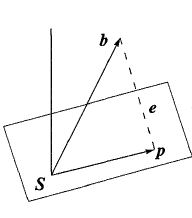
\includegraphics{week5/projection}
\caption{The projection of $\bm b$ onto a subspace $\bm S:=\mathcal{C}(\bm A)$.}\label{figure_12.2}
\end{figure}
\begin{definition}[Projection]
Let $\bm S\in\mathbb{R}^{m}$ be a non-empty closed set and $\bm b\in\mathbb{R}^m$ be given. Then the projection of $\bm b$ onto the set $\bm S$ is the solution to
\[
\min_{\bm z\in\bm S}\|\bm z-\bm b\|_2^2,
\]
where we use notation $\Proj_{\bm S}(\bm b)$ to denote the projection of $\bm b$ onto $\bm S$.
\end{definition}
By definition, the projection of $\bm b$ onto the subspace $\mathcal{C}(\bm A)$ is given by 
\[
\Proj_{\mathcal{C}(\bm A)}(\bm b):=\bm A\bm x^*,\quad
\text{where }\bm x^*=\arg\min_{\bm x\in\mathbb{R}^n}\|\bm{Ax} - \bm b\|.
\]

\begin{definition}[Projection matrix]
Given the projection
\[
\Proj_{C(\bm A)}(\bm b):=\bm A\bm x^{*}=\bm A(\bm A\trans\bm A)^{-1}\bm A\trans\bm b,
\]
since $[\bm A(\bm A\trans\bm A)^{-1}\bm A\trans]\bm b$,
we call the projection operator $\bm P:=\bm A(\bm A\trans\bm A)^{-1}\bm A\trans$ as the \emph{projection matrix} of $\bm A$.
\end{definition}
\begin{definition}[Idempotent]
Let $\bm A$ be a \emph{square} matrix that satisfies $\bm A=\bm A\bm A$, then $\bm A$ is called an \emph{idempotent} matrix.
\end{definition}
Let's show that the projection matrix is \textit{idempotent}:
\[
\begin{aligned}
\bm P^{2}&=\bm A(\bm A\trans\bm A)^{-1}\bm A\trans\bm A(\bm A\trans\bm A)^{-1}\bm A\trans\\
&=\bm A(\bm A\trans\bm A)^{-1}(\bm A\trans\bm A)(\bm A\trans\bm A)^{-1}\bm A\trans\\
&=\bm A(\bm A\trans\bm A)^{-1}\bm A\trans=\bm P.
\end{aligned}
\]

\subsubsection{Observations}
\begin{itemize}
\item
Suppose $\bm b\in \mathcal{C}(\bm A)$, i.e., $\exists \bm x$ s.t. $\bm{Ax}=\bm b$. Then the projection of $\bm b$ is exactly $\bm b$:
\[
\begin{aligned}
\bm{Pb}&=\bm A(\bm A\trans\bm A)^{-1}\bm A\trans(\bm b)\\
&=\bm A(\bm A\trans\bm A)^{-1}\bm A\trans(\bm{Ax})\\
&=\bm A(\bm A\trans\bm A)^{-1}(\bm A\trans\bm A)\bm x\\
&=\bm{Ax}=\bm b.
\end{aligned}
\]
\item
Assume $\bm A$ has only one column, say, $\bm a$. Then we have
\[\begin{aligned}
\bm x^{*}&=(\bm A\trans\bm A)^{-1}\bm A\trans\bm b=\frac{\bm a\trans\bm b}{\bm a\trans\bm a}\\
\bm A\bm x^{*}&=\bm{Pb}=\bm A(\bm A\trans\bm A)^{-1}\bm A\trans(\bm b)=\frac{\bm a\trans\bm b}{\bm a\trans\bm a}\times\bm a=\frac{\bm a\trans\bm b}{\|\bm a\|^2}\times\bm a
\end{aligned}
\]
More interestingly, 
\[\frac{\bm a\trans\bm b}{\|\bm a\|^2}\times\bm a=\frac{\|\bm a\|\|\bm b\|\cos\theta}{\|\bm a\|^2}\times\bm a=\|\bm b\|\cos\theta\times\frac{\bm a}{\|\bm a\|}\]
which is the projection of $\bm b$ onto a line $\Span\{\bm a\}$. (Shown in figure (\ref{Fig:6:3}).)
\begin{figure}[H]
\centering
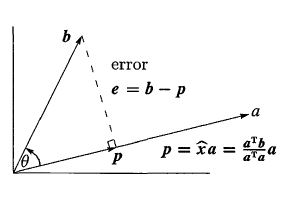
\includegraphics[width=10cm]{week5/projection_line}
\caption{The projection of $\bm b$ onto a line $\bm a$.}
\label{Fig:6:3}
\end{figure}
More generally, we can write the projection of $\bm b$ onto the line $\Span\{\bm a\}$ as:
\[
\Proj_{\Span\{\bm a\}}(\bm b)=\frac{\inp{\bm a}{\bm b}}{\inp{\bm a}{\bm a}}\bm a
\]
\paragraph{Changing an Orthogonal Basis}
Note that the error $\bm b-\Proj_{\Span\{\bm a\}}(\bm b)$ is perpendicular to $\bm a$, and $\bm b-\Proj_{\Span\{\bm a\}}(\bm b)\in\Span\{\bm a,\bm b\}.$

If we define $\bm b'=\bm b-\Proj_{\Span\{\bm a\}}(\bm b)$, then it's easy to check that $\Span\{\bm a,\bm b'\}=\Span\{\bm a,\bm b\}$ and $\bm a\perp\bm b'$. 

Hence, we convert the basis $\{\bm a,\bm b\}$ into another basis $\{\bm a,\bm b'\}$ such that the elements are orthogonal to each other. For general subspace we could also use this approach to obtain an orthogonal basis, which will be discussed in next lecture. 
\end{itemize}










%\chapter{Week5}

\section{Friday}\index{week5_Friday_lecture}
This lecture has two goals. The first is to see \emph{how orthogonality makes it easy to find projection matrix $\bm P$ and the projection $\Proj_{C(\bm A)}\bm b$}. \textit{Orthogonality makes the product $\bm A\trans\bm A$ a diagonal matrix}. The second goal is to \emph{show how to construct orthogonal vectors}. For matrix $\bm A=\begin{bmatrix}
a_1&a_2&\dots&a_n
\end{bmatrix}$, the columns may not be orthogonal. Then we convert $a_1,\dots,a_n$ to orthogonal vectors, which will be the columns of a new matrix $\bm Q$.
\subsection{Orthonormal basis}
The vectors $\bm q_1,\dots,\bm q_n$ are \emph{orthogonal} when their inner product $\inp{\bm q_i}{\bm q_j}$ are zero. ($i\ne j$.) With one more step--just divide each vector by its length, then the vectors become \emph{orthogonal unit vectors}. Their lengths are all 1. Then its basis is called \emph{orthonormal}.
\begin{definition}[orthonormal]
The vectors $\bm q_1,\dots,\bm q_n$ are \emph{orthonormal} if
\[
\inp{\bm q_i}{\bm q_j}=\begin{cases}
0&\text{when $i\ne j$}\qquad\text{(\emph{orthogonal} vectors)},\\
1&\text{when $i=j$}\qquad\text{(\emph{unit} vectors: $\|\bm q_i\|=1$)}.
\end{cases}
\]
Moreover, if $\bm q_1,\dots,\bm q_n$ are \emph{orthonormal}, then the basis $\{\bm q_1,\dots,q_n\}$ is called \emph{orthonormal basis}.
\end{definition}
\begin{example}
Unit vectors $\bm e_1=\begin{pmatrix}
1\\0\\\vdots\\0
\end{pmatrix},\bm e_2=\begin{pmatrix}
0\\1\\\vdots\\0
\end{pmatrix},\dots,\bm e_n=\begin{pmatrix}
0\\0\\\vdots\\1
\end{pmatrix}$ is an \textit{orthonormal basis} for $\mathbb{R}^{n}$.
\end{example}
If we want to express vector $\bm b$ as a linear combination of arbitrary basis $\{\bm q_1,\bm q_2,\dots,\bm q_n\}$, what should you do?\\
\textit{Answer:} To solve the system $\bm{Ax}=\bm b$, where $\bm A=\begin{bmatrix}
\bm q_1&\bm q_2&\dots&\bm q_n
\end{bmatrix}$.\\
What if $\{\bm q_1,\bm q_2,\dots,\bm q_n\}$ form an \emph{orthogonal} basis? How to find solution $\bm x$ s.t. 
\[
\bm b=x_1\bm q_1+x_2\bm q_2+\dots+x_n\bm q_n?
\]
\textit{Answer}: We just do the inner product of each $\bm q_i$ with $\bm b$ to get the coefficient $x_i$:
\[
\begin{aligned}
\inp{\bm q_i}{\bm b}&=x_1\inp{\bm q_i}{\bm q_1}+x_2\inp{\bm q_i}{\bm q_2}+\dots+x_n\inp{\bm q_i}{\bm q_n}\\
&=x_i\inp{\bm q_i}{\bm q_i}=x_i
\end{aligned}
\]
Since $x_i=\inp{\bm q_i}{\bm b}$, we could express $\bm b$ as:
\[
\bm b=\sum_{i=1}^{n}\inp{\bm q_i}{\bm b}\bm q_i.
\]
In this case, since $\{\bm q_1,\bm q_2,\dots,\bm q_n\}$ forms a basis, the columns of $\bm A$ must be ind. Hence $\bm A$ is invertible, then we get the solution to $\bm{Ax}=\bm b$:
\begin{equation}
\bm x=\bm A^{-1}\bm b.
\end{equation}
\begin{definition}[matrix with orthonormal columns]\qquad\\
Define $\bm Q=\begin{bmatrix}
q_1&q_2&\dots&q_n
\end{bmatrix}$. If vectors $\bm q_1,\dots,\bm q_n$ are \emph{orthonormal}, then we say $\bm Q$ is a matrix with \emph{orthonormal} columns.
\begin{remark}
Note that a matrix with \emph{orthonormal} columns is often denoted as $\bm Q$.
\end{remark}
\end{definition}
Such matrix \emph{is easy to work with} because we have:
\begin{equation}\label{eq:easy_to_work}
\bm Q\trans\bm Q=\begin{pmatrix}
\bm q_1\trans\\\bm q_2\trans\\\dots\\\bm q_n\trans
\end{pmatrix}\begin{pmatrix}
\bm q_1&\bm q_2&\dots&\bm q_n
\end{pmatrix}=\begin{pmatrix}
\bm q_1\trans\bm q_1&&\\
&\ddots&\\
&&\bm q_n\trans\bm q_n
\end{pmatrix}=\bm I.
\end{equation}
\begin{remark}
Note that a matrix with orthonormal columns $\bm Q$ is \textit{not required to be square}! Moreover, $\{\bm q_1,\dots,\bm q_n\}$ in $\bm Q$ is \textit{not required to form a basis}.
\end{remark}
\begin{definition}[orthogonal matrix]
An \emph{square} that is a \textit{matrix with orthonormal columns} is called \emph{othogonal matrix}.
\end{definition}
\begin{example}\qquad\\
If $\bm Q$ is a orthogonal matrix, while $\bm{\hat\bm Q}$ is a matrix with orthonormal columns that is \emph{not square}. Do the products $\bm Q\bm Q\trans$ and $\bm{\hat Q}\bm{\hat Q\trans}$ always be \textit{identity matrix}?\\
\textit{Answer}:
\begin{itemize}
\item
$\bm Q\bm Q\trans$ is always \textit{identity matrix}. According to equation (\ref{eq:easy_to_work}), we have $\bm Q\trans\bm Q=\bm I$.\\ Hence $\bm Q\trans$ is the left inverse of square matrix $\bm Q$.\\ Hence $\bm Q^{-1}=\bm Q\trans\implies\bm Q\bm Q\trans=\bm Q\bm Q^{-1}=\bm I$.\\
Moreover, solving $\bm{Qx}=\bm b$ is equivalent to $\bm x=\bm Q^{-1}\bm b=\bm Q\trans\bm b$, which is \textit{exactly} 
\[
\bm x=\begin{bmatrix}
\inp{\bm q_1}{\bm b}\\\inp{\bm q_2}{\bm b}\\\vdots\\\inp{\bm q_n}{\bm b}
\end{bmatrix}.
\]
\item
But the product $\bm \hat Q\bm \hat Q\trans$ will never be identity matrix. Assume $\bm \hat Q$ is a $m\times n$ matrix. ($m\ne n$.) Then it's easy to verify that $\rank(\bm \hat Q\bm \hat Q\trans)=\rank(\bm\hat Q)$.\\ Since $\bm\hat Q$ has orthonormal columns, the columns of $\bm\hat Q$ are ind. Hence $\rank(\bm\hat Q)=n$.\\ But $\rank(\bm \hat Q\bm \hat Q\trans)=\rank(\bm\hat Q)=n\ne m=\rank(\bm I_{m})$.\\
Moreover, if $\bm\hat Q$ has only one column $\bm\hat q$, then $\bm \hat Q\bm \hat Q\trans=\bm\hat q\bm\hat q\trans=\rank(1)\ne \bm I_{m}$.
\end{itemize}
\end{example}
\begin{proposition}\quad\\
If $\bm Q$ has orthonormal columns, then it \textit{leaves lengths unchanged}, in other words,
\[
\text{\emph{Same length}}\qquad\qquad
\|\bm{Qx}\|=\|\bm x\|\quad\text{for every vector $\bm x$.}
\]
Also, $\bm Q$ preserves inner products for vectors:
\[
\inp{\bm{Qx}}{\bm{Qy}}=\inp{\bm x}{\bm y}\quad\text{for every vectors $\bm x$ and $\bm y$.}
\]
\end{proposition}
\begin{proof}[Proofoutline.]
$\|\bm{Qx}\|^2=\|\bm x\|^2$ because
\[\begin{aligned}
\inp{\bm{Qx}}{\bm{Qx}}&=\bm x\trans\bm Q\trans\bm Q\bm x=\bm x\trans(\bm Q\trans\bm Q)\bm x\\
&=\bm x\trans\bm I\bm x=\bm x\trans\bm x
\end{aligned}
\]
Hence we have $\|\bm{Qx}\|=\|\bm x\|$. Just using $\bm Q\trans\bm Q=\bm I$, we can derive $\inp{\bm{Qx}}{\bm{Qy}}=\inp{\bm x}{\bm y}$.
\end{proof}
Orthogonal matrices are excellent for computations, since numbers can never grow too large when lengths of vectors are fixed.\\
In particular, if $\bm Q\in\mathbb{R}^{m\times n}$ has orthonormal columns, the least square problem is easy:\\
Although $\bm{Qx}=\bm b$ may not have a solution, but the normal equation
\[
\bm Q\trans\bm Q\bm \hat x=\bm Q\trans\bm b
\]
must have a unique solution $\bm\hat x=\bm Q\trans\bm b$. Why? Since $\bm Q\trans\bm Q=\bm I$, we derive $\bm\hat x=\bm Q\trans\bm Q\bm \hat x=\bm Q\trans\bm b$.\\
\emph{\textit{\Large Summary:}}\\
Hence the \emph{least squares solution} to $\bm{Qx}=\bm b$ is $\bm\hat x=\bm Q\trans\bm b$. In other words, $\bm Q\bm Q\trans\bm b\approx \bm b$. \emph{The projection matrix is} $\bm P=\bm Q\bm Q\trans$. Note that the projection $\Proj_{\col(\bm Q)}(\bm b)=\bm Q\bm Q\trans\bm b$ doesn't equal to $\bm b$ in general.\\
For general $\bm A$, the projection matrix is $\bm P=\bm A(\bm A\trans\bm A)^{-1}\bm A\trans$.
\subsection{Gram-Schmidt Process}
``Orthogonal is good''. So our goal for this section is: \textit{Given ind. vectors, how to make them orthonormal?}\\
We start with three ind. vectors $\bm a,\bm b,\bm c$ in $\mathbb{R}^{3}$. In order to construct orthonormal vectors, firstly we construct three \emph{orthogonal} vectors $\bm A,\bm B,\bm C$. Then we divide $\bm A,\bm B,\bm C$ by their lengths to get three \emph{orthonormal} vectors $\bm q_1=\frac{\bm A}{\|\bm A\|},\bm q_2=\frac{\bm B}{\|\bm B\|},\bm q_3=\frac{\bm C}{\|\bm C\|}.$
\newpage
Firstly we set $\bm A=\bm a$. The next vector $\bm B$ must be perpendicular to $\bm A$.\\ Look at the figure (\ref{figure_13.1}) below, We find that $\bm B=\bm b-\Proj_{\bm A}(\bm b)$. Hence
\[
\text{\emph{First Gram-Schmidt step}}\qquad
\bm B=\bm b-\frac{\inp{\bm A}{\bm b}}{\inp{\bm A}{\bm A}}\bm A.
\]
\begin{figure}[H]
\centering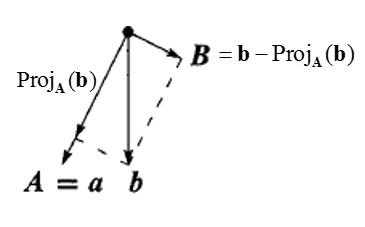
\includegraphics[width=5cm]{week5/gram}
\caption{Subtract projection to get $\bm B=\bm b-\Proj_{\bm A}\bm b$.}\label{figure_13.1}
\end{figure}
You can take inner product between $\bm A$ and $\bm B$ to verify that $\bm A$ and $\bm B$ are orthogonal in Figure (\ref{figure_13.1}). Note that $\bm B$ is not zero (otherwise $\bm a$ and $\bm b$ would be dep. We will show it later.)\\\\
Then we want to construct vector $\bm C$. $\bm C$ is not a linear combination of $\bm A$ and $\bm B$. (Because $\bm c$ is not a linear combination of $\bm a$ and $\bm b$.) But most likely $\bm c$ is \emph{not} perpendicular to $\bm A$ and $\bm B$. Hence we \textit{subtract $\bm c$ off its projections onto the space of $\bm A$ and $\bm B$.} to get $\bm C$:
\[
\text{\emph{Next Gram-Schmidt step}}\qquad\begin{aligned}
\bm C&=\bm c-\Proj_{\Span\{\bm A,\bm B\}}(\bm c)\\
&=\bm c-\Proj_{\bm A}(\bm c)-\Proj_{\bm B}(\bm c)\\
&=\bm c-\frac{\inp{\bm A}{\bm c}}{\inp{\bm A}{\bm A}}\bm A-\frac{\inp{\bm B}{\bm c}}{\inp{\bm B}{\bm B}}\bm B.
\end{aligned}
\]
\begin{figure}[H]\centering
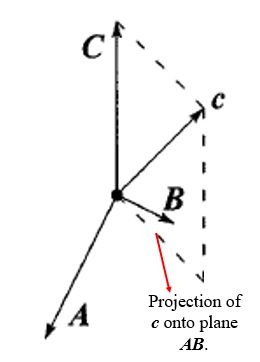
\includegraphics[width=5cm]{week5/nextgram}
\end{figure}
Finally we get $\bm A,\bm B,\bm C$. Orthonormal vectors $\bm q_1,\bm q_2,\bm q_3$ are obtained by dividing their lengths (shown in Figure (\ref{Final_gram})):
\begin{figure}[H]\centering
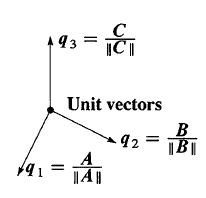
\includegraphics[width=5cm]{week5/finalgram}
\caption{Final Gram-Schmidt step}
\label{Final_gram}
\end{figure}
Next we show an example of Gram-Schmidt step:
\begin{example}
How to construct orthonormal vectors for $\bm a=\begin{pmatrix}
1\\0\\1
\end{pmatrix},\bm b=\begin{pmatrix}
1\\0\\0
\end{pmatrix},\bm c=\begin{pmatrix}
2\\1\\0
\end{pmatrix}?$\\
\begin{itemize}
\item
Firstly we set $\bm A=\bm a=\begin{pmatrix}
1\\0\\1
\end{pmatrix}$.
\item
\[
\begin{aligned}
\bm B&=\bm b-\Proj_{\bm A}(\bm b)=\bm b-\frac{\inp{\bm A}{\bm b}}{\inp{\bm A}{\bm A}}\bm A\\
&=\begin{pmatrix}
1\\0\\0
\end{pmatrix}-\begin{pmatrix}
1\\0\\1
\end{pmatrix}\trans\begin{pmatrix}
1\\0\\0
\end{pmatrix}2^{-1}\begin{pmatrix}
1\\0\\1
\end{pmatrix}\\
&=\begin{pmatrix}
\frac{1}{2}\\0\\-\frac{1}{2}
\end{pmatrix}
\end{aligned}
\]
\item
\[
\begin{aligned}
\bm C&=\bm c-\Proj_{\bm A}(\bm c)-\Proj_{\bm B}(\bm c)=\bm c-\frac{\inp{\bm A}{\bm c}}{\inp{\bm A}{\bm A}}\bm A-\frac{\inp{\bm B}{\bm c}}{\inp{\bm B}{\bm B}}\bm B\\
&=\begin{pmatrix}
2\\1\\0
\end{pmatrix}-\begin{pmatrix}
1\\0\\1
\end{pmatrix}\trans\begin{pmatrix}
2\\1\\0
\end{pmatrix}2^{-1}\begin{pmatrix}
1\\0\\1
\end{pmatrix}-\begin{pmatrix}
\frac{1}{2}\\0\\-\frac{1}{2}
\end{pmatrix}\trans\begin{pmatrix}
2\\1\\0
\end{pmatrix}(\frac{1}{2})^{-1}\begin{pmatrix}
\frac{1}{2}\\0\\-\frac{1}{2}
\end{pmatrix}\\
&=\begin{pmatrix}
0\\1\\0
\end{pmatrix}
\end{aligned}
\]
Hence we obtain our orthonormal vectors:
\[
\bm q_1=\frac{\bm A}{\|\bm A\|}
=\begin{pmatrix}
\frac{1}{\sqrt 2}\\0\\\frac{1}{\sqrt 2}
\end{pmatrix},
,\bm q_2=\frac{\bm B}{\|\bm B\|}
=\begin{pmatrix}
\frac{1}{\sqrt 2}\\0\\-\frac{1}{\sqrt 2}
\end{pmatrix}
,\bm q_3=\frac{\bm C}{\|\bm C\|}
=\begin{pmatrix}
0\\1\\0
\end{pmatrix}
\]
\end{itemize}
And we derive the orthogonal matrix $\bm Q$:
\[
Q=\begin{pmatrix}
\frac{1}{\sqrt 2}&\frac{1}{\sqrt 2}&0\\0&0&1\\
\frac{1}{\sqrt 2}&-\frac{1}{\sqrt 2}&0
\end{pmatrix}
\]
\end{example}
But when will the Gram-Schmidt process ``fail''? Let's describle this process in general case, then we answer this question.\\
\subsubsection{Gram-Schmidt process in general case}
\emph{Input: }Ind. vectors $a_1,\dots,a_n$.\\
Firstly we want to construct orthogonal vectors $\bm A_1,\dots,\bm A_n$.\\
In step $j\in\{1,\dots,n\}$, we want to compute $a_j$ minus its projection in the space spanned by $\{\bm A_1,\bm A_2,\dots,\bm A_{j-1}\}$:
\[
\begin{aligned}
\bm A_j&=a_j-\Proj_{\Span\{\bm A_1,\bm A_2,\dots,\bm A_{j-1}\}}(a_j)\\
&=a_j-\Proj_{\bm A_1}(a_j)-\Proj_{\bm A_2}(a_j)-\dots-\Proj_{\bm A_{j-1}}(a_j)\\
&=a_j-\frac{\inp{\bm A_1}{a_j}}{\inp{\bm A_1}{\bm A_1}}\bm A_1-\frac{\inp{\bm A_2}{a_j}}{\inp{\bm A_2}{\bm A_2}}\bm A_2-\dots-\frac{\inp{\bm A_{j-1}}{a_j}}{\inp{\bm A_{j-1}}{\bm A_{j-1}}}\bm A_{j-1}
\end{aligned}
\]
After we get $\bm A_1,\dots,\bm A_n$, we can construct orthonormal vectors:
\[
\bm q_j=\frac{\bm A_j}{\|\bm A_j\|}\quad\text{for }j=1,2,\dots,n.
\]
So when do this process fail? When $\exists j$ such that $\bm A_j=\bm 0$, we cannot continue this process anymore.
\begin{proposition}
$\bm A_j\ne\bm0$ for $\forall j$ if and only if $a_1,a_2,\dots,a_n$ are ind.
\end{proposition}
\begin{proof}[Proofoutline.]
$\bm A_j=\bm0\Longleftrightarrow
a_j=\Proj_{\Span{\bm A_1,\dots,\bm A_{j-1}}}(a_j)$\\
Hence we only need to prove $\exists j$ s.t. $\bm A_j=\bm 0$ if and only if $a_1,a_2,\dots,a_n$ are dep.\\
\textit{Sufficiency. }Given $\bm A_j=\bm0$, then $a_j=\Proj_{\Span{\bm A_1,\dots,\bm A_{j-1}}}(a_j)\in\Span\{\bm A_1,\dots,\bm A_{j-1}\}$. It's easy to verify that $\Span\{\bm A_1,\dots,\bm A_{j-1}\}=\Span\{a_1,\dots,a_{j-1}\}$. Hence $a_j\in\Span\{a_1,\dots,a_{j-1}\}$. \\Hence $a_1,\dots,a_j$ are dep. Thus $a_1,\dots,a_n$ are dep.\\\\
\textit{Necessity. }Given $a_1,a_2,\dots,a_n$ are dep. Then obviously, $a_n\in\Span\{a_1,\dots,a_{n-1}\}$. It's easy to verify that $a_n=\Proj_{\Span\{a_1,\dots,a_{n-1}\}}(\bm a_n)$. Thus $a_n=\Proj_{\Span\{\bm A_1,\dots,\bm A_{n-1}\}}(\bm a_n)\implies \bm A_n=\bm0$.
\end{proof}
\subsection[The Factorization $A=QR$.]{The Factorization $\bm A=\bm{QR}$}
We know Gaussian Elimination leads to \textit{LU decomposition}; in fact, Gram-Schmidt process leads to \textit{QR factorization}. These two decomposition methods are quite important in LA, let's discuss QR factorization briefly:\\
Given a matrix $\bm A=\begin{bmatrix}
\bm a&\bm b&\bm c
\end{bmatrix}$, we finally end with a matrix $\bm Q=\begin{bmatrix}
\bm q_1&\bm q_2&\bm q_3
\end{bmatrix}$.\\ How are these two matrix related? \\
\textit{Answer:} Since the linear combination of $\bm a,\bm b,\bm c$ leads to $\bm q_1,\bm q_2,\bm q_3$ (vice versa), there must be a third matrix connecting $\bm A$ to $\bm Q$. This third matrix is the triangular $\bm R$ such taht $\bm A=\bm{QR}$.\\
In general case, $\bm a_1,\dots,\bm a_k$ are combinations of $\bm q_1,\dots,\bm q_k$ at every step.\\ (In general suppose $\bm A=\begin{bmatrix}
\bm a_1&\bm a_2&\dots&\bm a_n
\end{bmatrix}, \bm Q=\begin{bmatrix}
\bm q_1&\bm q_2&\dots&\bm q_n
\end{bmatrix}$)
\newpage
Let's discuss a specific example to show how to do factorization.
\begin{example}
Given $\bm A=\begin{bmatrix}
\bm a&\bm b&\bm c
\end{bmatrix}$, whose columns are ind. We can write $\bm A$ as:
\[
\bm A=\begin{bmatrix}
\bm q_1&\bm q_2&\bm q_3
\end{bmatrix}\begin{bmatrix}
\bm q_1\trans\bm a&\bm q_1\trans\bm b&\bm q_1\trans\bm c\\0&\bm q_2\trans\bm b&\bm q_2\trans\bm c\\0&0&\bm q_3\trans\bm c
\end{bmatrix}
\]
where $\bm q_1,\bm q_2,\bm q_3$ are \emph{orthonormal}.\\
We define $\bm R\triangleq\begin{bmatrix}
\bm q_1\trans\bm a&\bm q_1\trans\bm b&\bm q_1\trans\bm c\\0&\bm q_2\trans\bm b&\bm q_2\trans\bm c\\0&0&\bm q_3\trans\bm c
\end{bmatrix}, \bm Q\triangleq\begin{bmatrix}
\bm q_1&\bm q_2&\bm q_3
\end{bmatrix}$.\\
Hence $\bm A$ could be factorized into:
\[
\bm A=\bm{QR}
\]
where $\bm R$ is upper triangular, $\bm Q$ is a matrix with orthonormal columns.
\end{example}
We have a theorem about QR faactorization (without proof):
\begin{theorem}
Every $m\times n$ matrix $\bm A$ with ind. columns can be factorized as
\[
\bm A=\bm{QR}
\]
where $\bm Q$ is a matrix with \textit{orthonormal columns}, $\bm R$ is a upper triangular matrix (always square).
\end{theorem}
We postmultiply $\bm Q\trans$ both sides for $\bm A=\bm{QR}$ to obtain $\bm R=\bm Q\trans\bm A$. In fact, the inverse of $\bm R$ always exists.
\enlargethispage{1cm}
\begin{proof}
suppose $\bm A=\begin{bmatrix}
\bm a_1&\bm a_2&\dots&\bm a_n
\end{bmatrix}, \bm Q=\begin{bmatrix}
\bm q_1&\bm q_2&\dots&\bm q_n
\end{bmatrix}$.
 Thus we derive \[\bm R=\bm Q\trans\bm A=\begin{bmatrix}
\bm q_1\trans\bm a_1&\bm q_1\trans\bm a_2&\dots&\bm q_1\trans\bm a_n\\
0&\bm q_2\trans\bm a_2&\dots&\bm q_2\trans\bm a_n\\
\vdots&\vdots&\ddots&\vdots\\
0&0&\dots&\bm q_n\trans\bm a_n
\end{bmatrix}
\]
For every step $j$ we have 
\[\bm A_j=\bm a_j-\Proj_{\Span\{a_1,\dots,a_{j-1}\}}( \bm a_j),\qquad \bm q_j=\frac{\bm A_j}{\|\bm A_j\|}.
\]
Since $\inp{\bm A_j}{\bm a_j}=\inp{\bm a_j}{\bm a_j}-\inp{\Proj_{\Span\{a_1,\dots,a_{j-1}\}}(\bm a_j)}{\bm a_j}=\|a_j\|^2-\|\Proj_{\Span\{a_1,\dots,a_{j-1}\}}(\bm a_j)\|^2>0$, we have $\inp{\bm q_j}{\bm a_j}=\frac{\inp{\bm A_j}{\bm a_j}}{\|\bm A_j\|}>0.$ Hence the diagonal of $\bm R$ are all positive. Hence this triangular matrix is \textit{invertible.}
\end{proof}
\begin{proposition}
If $\bm A=\bm{QR}$, then we have a simple way to solve $\bm A\trans\bm A\bm x=\bm A\trans\bm b$.
\end{proposition}
\begin{proof}[Explain:]
Since we have
\[
\begin{aligned}
\bm A\trans\bm A\bm x&=\bm R\trans\bm Q\trans\bm Q\bm R\bm x=\bm R\trans\bm R\bm x\\
\bm A\trans\bm b&=\bm R\trans\bm Q\trans\bm b
\end{aligned}
\]
it's equivalent to solve $\bm R\trans\bm R\bm x=\bm R\trans\bm Q\trans\bm b$.\\
Sicne $\bm R$ is \textit{invertible}, we solve by substitution to get
\[
\bm x=(\bm R\trans\bm R)^{-1}\bm R\trans\bm Q\trans\bm b=\bm R^{-1}\bm Q\trans\bm b.
\]
\end{proof}\newpage
\subsection{Function Space}
Sometimes we may also discuss orthonormal basis and Gram-Schmidt process on function space. There is a simple example:
\begin{example}
For subspace $\Span\{1,x,x^2\}\subset C[-1,1]$, firstly, how to define orthogonal for the basis $\{1,x,x^2\}$?\\
\textit{Pre-requisite: }Inner product.
\[
\inp{f}{g}=\int_{a}^{b}fg\diff x \text{ for $f,g\in C[a,b]$.}\qquad
\|f\|^2=\int_{a}^{b}f^2\diff x
\]
If we have defined inner product, then we can talk about \textit{orthogonality} for $\{1,x,x^2\}$. It's easy to verify that
\[
\inp{1}{x}=0\quad\inp{x}{x^2}=0\quad\inp{1}{x^2}=\frac{2}{3}.
\]
If we do the Gram-Schmidt Process, we obtain:
\[
\bm A=1,\qquad\bm B=x,\qquad
\bm C=x^2-\frac{\inp{1}{x^2}}{\inp{1}{1}}1-\frac{\inp{x}{x^2}}{\inp{x}{x}}x=x^2-\frac{1}{3}
\]
$\bm A,\bm B,\bm C$ are \textit{orthogonal}. We can divide their length to obtain orthonormal basis:
\[
\begin{aligned}
\bm q_1&=\frac{\bm A}{\|\bm A\|}=\frac{1}{\sqrt{\int_{-1}^{1}1^2\diff x}}=\frac{1}{2}\qquad\\
\bm q_2&=\frac{\bm B}{\|\bm B\|}=\frac{x}{\sqrt{\int_{-1}^{1}x^2 \diff x}}=\frac{x}{2/3}=\frac{3}{2}x\qquad\\
\bm q_3&=\frac{\bm C}{\|\bm C\|}=\frac{x^2-\frac{1}{3}}{\sqrt{\int_{-1}^{1}(x^2-\frac{1}{3})^2 \diff x}}=\frac{x^2-\frac{1}{3}}{\frac{8}{45}}=\frac{45x^2-15}{8}
\end{aligned}
\]
Hence $\{\bm q_1,\bm q_2, \bm q_3\}$ is the orthonormal basis for $\Span\{1,x,x^2\}$.
\end{example}
\begin{example}
Consider the collection $\mathcal{F}$ of functions defined on $[0,2\pi]$, where
\[
\mathcal{F}:=\{1,\cos x,\sin x,\cos 2x,\sin 2x,\dots,\cos mx,\sin mx,\dots\}
\]
Using various trigonometric identities, we can show that if $f$ and $g$ are \emph{distinct}(different) functions in $\mathcal{F}$, we have $\int_{0}^{2\pi}fg\diff x=0$. For example,
\[
\inp{\sin x}{\sin 2x}=\int_{0}^{2\pi}\sin x\sin 2x\diff x=\int_{0}^{2\pi}\frac{1}{2}(\cos x-\cos 3x)\diff x=0.
\]
And moreover, if $f=g$, we have $\int_{0}^{2\pi}f^2\diff x=\pi$. For example,
\[
\inp{\sin 5x}{\sin 5x}=\int_{0}^{2\pi}\sin^2 5x\diff x=\int_{0}^{2\pi}\frac{1}{2}(1+\cos 10x)\diff x=\pi.
\]
In conclusion, the collection $\{1,\sin mx,\cos mx\}$ for $k=1,2,\dots$ are \textit{orthogonal} in $C[0,2\pi]$. Note that this set is \emph{not orthonormal}!
\end{example}
This example motivates the fourier transformation:
\subsection{Fourier Series}
The Fourier series of a function is its expansion into sines and cosines:
\[
f(x)=a_0+a_1\cos x+b_1\sin x+a_2\cos 2x+b_2\sin 2x+\dots
\]
where $f(x)\in C[0,2\pi]$. We have an orthogonal basis! But what kind of function could be expressed in this way? There is a theorem for this condition (without proof):
\begin{theorem}
If a function $f$ have the finite length in its function space $C[a,b]$, then it could be expressed as \textit{fourier series}.
\end{theorem}
But how to compute the coefficients $a_i's$ and $b_j's$? The key is orthogonality! For example, in order to get $a_1$, we just do the inner product between $f(x)$ and $\cos x$:
\begin{figure}[H]\centering
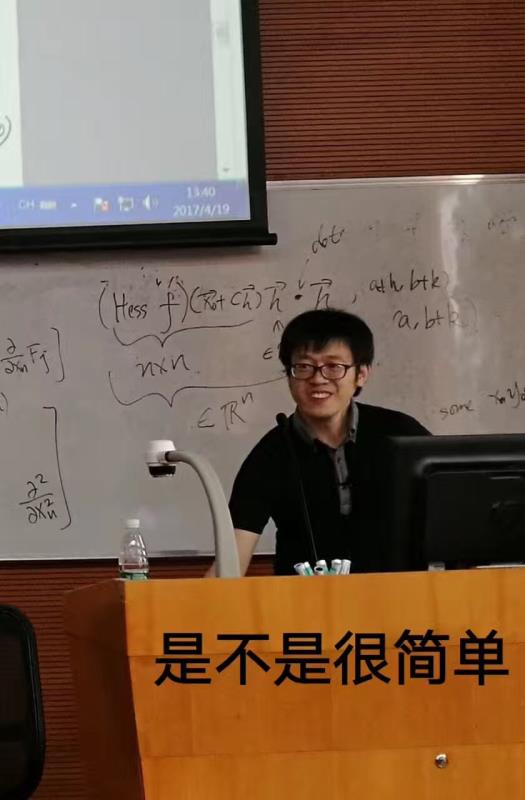
\includegraphics[width=5cm]{week5/1810645243}
\caption{Enjoy fourier series!}
\end{figure}
\[
\inp{f(x)}{\cos x}=a_1\inp{\cos x}{\cos x}+0
\implies
a_1=\frac{\inp{f(x)}{\cos x}}{\inp{\cos x}{\cos x}}=\frac{1}{\pi}\int_{0}^{2\pi}f(x)\cos x\diff x
\]
Similarly we derive 
\[
a_m=\frac{1}{\pi}\int_{0}^{2\pi}f(x)\cos mx\diff x
\qquad
b_m=\frac{1}{\pi}\int_{0}^{2\pi}f(x)\sin mx\diff x.
\]
\section{Assignment Six}\index{Assignment_Six}
\begin{enumerate}
\item
Find the \textit{determinant} of the linear transformation $T(f(t))=f(3t-2)$ from $\mathbb{P}_2$ to $\mathbb{P}_2$.
\item
Suppose that $\bm A$ is a $m$ by $n$ real matrix. And suppose that $\bm{Ax}=\bm0$ and $\bm A\trans\bm y=2\bm y.$ Show that $\bm x$ is \textit{orthogonal} to $\bm y$.
\item
State and justify whether the following three statements are True or False (give an
example in either case):
\begin{enumerate}
\item
$\bm Q^{-1}$ is an \textit{orthogonal} matrix when $\bm Q$ is an \textit{orthogonal} matrix.
\item
If $\bm Q$ (a $m$ by $n$ matrix with $m>n$) has \textit{orthonormal columns}, then $\|\bm{Qx}\|=\|\bm x\|.$
\item
If $\bm Q$ (a $m$ by $n$ matrix with $m>n$) has \textit{orthonormal columns}, then $\|\bm{Q\trans\bm y}\|=\|\bm y\|.$
\end{enumerate}
\item
Let us make $P(\mathbb{R})$ into an \textit{inner product space} using the inner product
\[
\inp{p}{q}=\int_{-1}^{1}p(x)q(x)\diff x
\]
Recall that we say a function is \textit{even} if $\forall x$ we have $f(-x)=f(x)$ and \textit{odd} if $\forall x$ we have $f(-x)=-f(x).$\\
$W_1$ corresponds to the set of \textit{odd polynomials} and $W_2$ the set of \textit{even polynomials}. Show that $W_1=W_2^{\perp}.$
\item
Let $\bm V=\mathbb{R}^3,$ $\bm U$ the \textit{orthogonal complement} to $\Span\left\{\begin{pmatrix}
1\\2\\-5
\end{pmatrix}\right\}$. Find an \textit{orthonormal basis}
of $\bm U$.
\item
Find the best line $C+Dt$ to fit $b=4,2,-1,0,0$ at times $t=-2,-1,0,1,2$.
\end{enumerate}
%\include{week6/Lecture_1}
%\include{week6/Lecture_2}

\chapter{Week6}

\section{Tuesday}\index{week6_Tuesday_lecture}
\subsection{Summary of last two weeks}
In the first two weeks, we have learnt how to solve linear system of equations $\bm{Ax}=\bm b$. To understand this equation better, we learn the definition for matrices and vector space. Matrices calculation involve vectors, the columns $\bm{Ax}$ are linear combination of $n$ vectors--columns of $\bm{A}$. \\
\subsubsection{Determinants}
And then we learn how to describle the \emph{quantity of a matrix}--determinant. The determinant of a square matrix is a single number. That number contains an amazing amount of information about the matrix. There are three main points about determinant:
\begin{itemize}
\item
\textit{Determinants is related to invertibility, rank, eigenvalue, PSD$,\dots$}
\item
$\det(\bm{AB})=\det(\bm A)\det(\bm B).$
\item
\textit{The square matrix $\bm A$ is invertible} if and only if $\det(\bm A)\ne 0.$
\end{itemize}

\subsubsection{Linear Transformation}
Linear transfromation is another important topic. The matrix multiplication $T(\bm v)=\bm{Av}$ gives a lienar transformation. If we consider a vector as a point in a vector space, then \textit{the linear transformation allows movements in the space}. It ``transforms'' vector $\bm v$ to another vector $\bm{Av}$. In view of linear transformation, we can understand $\det(\bm{AB})=\det(\bm A)\det(\bm B)$ better:
\[
\det(\bm A)=\text{Volumn of $\bm{Ak}$, where $\bm k$ is a unit cube.}
\]
If we transform the $\bm k$ by $\bm A$ secondly by $\bm B$, actually, it has the same effect of transforming $\bm k$ by $\bm{BA}$.
\begin{figure}[H]
\centering
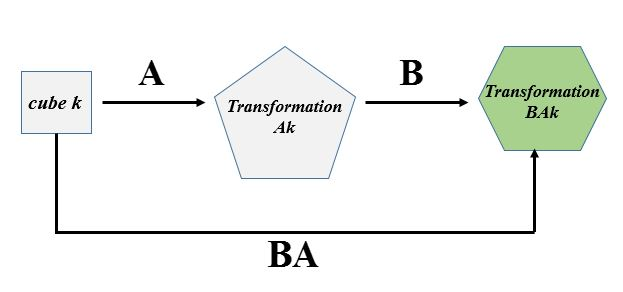
\includegraphics[width=10cm]{week6/determinant}
\caption{Transformation of a vector by $\bm A$, then by $\bm B$ has the same effect by $\bm{BA}$.}
\end{figure}
Hence if we denote the volumn on a graph, we find the volumn of $\bm B(\bm{Ak})$ is exactly the same as $(\bm{BA})\bm k$. Hence we have $\det(\bm B)\det(\bm A)=\det(\bm{BA})$.\\
Morevoer, $\det(\bm A)=0\Longleftrightarrow
\text{Volumn of $\bm{Ak}=0$}\Longleftrightarrow
\dim(\bm{Ak})=0.$\\
Cramer's Rule also has geometric meaning, which will not be talked in this lecture. (In big data age, people will not use cramer's rule frequently.)\\
Linear transformation has a matrix representation under certain basis. How to transform one basis into another basis? We have to use \textit{similar matrices as matrix representation}.
\subsubsection{Orthogonality}
Why we learn orthogonality? It has two motivations:
\begin{enumerate}
\item
Linear independence between vectors
$\Longleftrightarrow\text{Angle}\ne0\degree.$\\
Then we are interested in the special case:
orthogonal$\Longleftrightarrow\text{Angle}=90\degree$.
\item
Solving least squares (linear regression).\\
Input: $x =$age of propellant, Output: $y = $shear strength.\\
Our data contains $S=\{(x_1,y_1),\dots,(x_{n},y_{n})\}$, $n=20$ samples.\\
We want to find a best line that fit the data:
\begin{figure}[H]
\centering
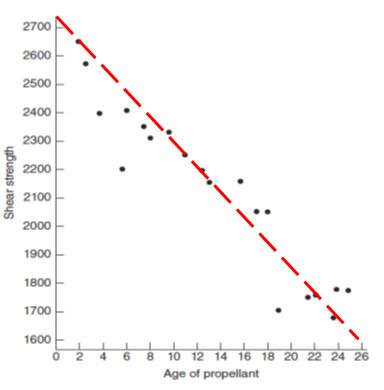
\includegraphics[width=5cm]{week6/regression}
\caption{The relationship between $x$ and $y$.}
\end{figure}
In other words, we want to find $\bm x$ s.t.
\[
    (\tikzmark{identity}{$\bm A$}\tikzmark[red]{G}{$\bm x$}
    \approx\tikzmark[purple]{C}{$\bm b$})
\]
\begin{tikzpicture}[overlay, remember picture,node distance =1.5cm]
    \node (identitydescr) [below left=of identity ]{age};
    \draw[,->,thick] (identitydescr) to [in=-90,out=90] (identity);
    \node[red] (Gdescr) [below =of G]{coefficient};
    \draw[red,->,thick] (Gdescr) to [in=-90,out=90] (G);
    
    \node[purple] (Cdescr) [below right =of C]{strength};
    \draw[purple,->,thick] (Cdescr) to [in=-90,out=90] (C.south);
\end{tikzpicture}
\end{enumerate}
\newpage
The general least square problem is given by:
\[
\min_{\bm x\in\mathbb{R}^{n}}\|\bm{Ax}-\bm b\|^2
\]
where $\bm b\in\mathbb{R}^{m}$.
\begin{itemize}
\item
If $m=n$, this optimization problem is converted into find the solution to equation $\bm{Ax}=\bm b$.
\item
Otherwise, the least square solution must satisfy $\frac{\partial }{\partial \bm x}\|\bm{Ax}-\bm b\|^2=\bm 0$.
\[
\implies\bm A\trans\bm A\bm x=\bm A\trans\bm b.\qquad\text{(\emph{normal equation.})}
\]
\end{itemize}
This potimization problem also has geometric meaning:
\begin{figure}[H]
\centering\includegraphics{week6/least_square}
\caption{Least square problem: find $\bm x$ such that $\bm{Ax}=\Proj_{\bm A}(\bm b).$}
\end{figure}
So you need to memorize we only need to find $\bm x$ such that $\bm{Ax}=\Proj_{\bm A}(\bm b)$.\\
But how to find $\Proj_{\bm A}(\bm b)$? You can write it as inner product:
\[
\Proj_{\bm A}(\bm b)=\bm A\frac{1}{\inp{\bm A}{\bm A}}\inp{\bm A}{\bm b}
=\bm A(\bm A\trans\bm A)^{-1}\bm A\trans\bm b.
\]
\begin{remark}
\begin{itemize}
\item
The projection of $\bm b$ onto a vector $\bm a$ is given by:
\[
\Proj_{\bm a}(\bm b)=\frac{\inp{\bm a}{\bm b}}{\inp{\bm a}{\bm a}}\bm a
\]
Since the factor $\frac{\inp{\bm a}{\bm b}}{\inp{\bm a}{\bm a}}$ is a scalar, you can also write the projection as:
\[
\Proj_{\bm a}(\bm b)=\bm a\frac{\inp{\bm a}{\bm b}}{\inp{\bm a}{\bm a}}
\]
\item
However, the projection of $\bm b$ onto a subspace $\{\bm{Ax}|\bm x\in\mathbb{R}^{n}\}$ is given by
\[
\Proj_{\bm A}(\bm b)=\bm A\frac{1}{\inp{\bm A}{\bm A}}\inp{\bm A}{\bm b}
\]
We \emph{cannot} write this projection as $\frac{1}{\inp{\bm A}{\bm A}}\inp{\bm A}{\bm b}\bm A$, since the factor $\frac{1}{\inp{\bm A}{\bm A}}\inp{\bm A}{\bm b}$ is a vector instead of a scalar.
\enlargethispage{1cm}
\end{itemize}
\end{remark}
The least square solution is given by
\[
\bm x=(\bm A\trans\bm A)^{-1}\bm A\trans\bm b.
\]
If $\bm A=\bm Q$, where $\bm Q$ is a \textit{orthogonal matrix}, then the solution is converted as 
\[
\bm x=\bm Q\trans\bm b.
\]
\subsection{Eigenvalues and eigenvectors}
\subsubsection{Why do we study eigenvalues and eigenvectors?}
\begin{itemize}
\item
\emph{Motivation 1: }If we consider matrices as the \textit{movements} (linear transformation) for \textit{vectors} in vector space. Then roughly speaking, \textit{eigenvalues} are the \textit{speed} of the movements, \textit{eigenvectors} are the \textit{direction} of the movements
\item
\emph{Motivation 2: }We know that linear transformation has different matrix representation for different basis. But which representation is \emph{simplest} for one linear transformation? This section gives us answer to this question.
\end{itemize}
When vectors are multiplied by A, almost all vectors change direction. If $\bm x$ has the same direction as $\bm{Ax}$, they are called \emph{eigenvectors}.
\[
\text{\emph{The key equation is }}\bm{Ax}=\lambda\bm x,\qquad\text{\emph{The numebr $\lambda$ is the eigenvalue of $\bm A$.}}
\]
\begin{definition}[Eigenvectors and Eigenvalues]
Let $\bm A$ be $n\times n$ matrix. A scalar $\lambda$ is an \emph{eigenvalue} of $\bm A$ iff $\exists$ a vector $\bm x\ne \bm 0$ s.t. $\bm{Ax}=\lambda \bm x$. The vector $\bm x$ is called an \emph{eigenvector} (corresponding to $\lambda$.)
\end{definition}
\begin{example}\qquad\\
\begin{gather*}
\bm A=\begin{bmatrix}
4&-2\\1&1
\end{bmatrix}\qquad\bm x=\begin{bmatrix}
2\\1
\end{bmatrix}\\
\bm{Ax}=\begin{bmatrix}
6\\3
\end{bmatrix}=3\begin{bmatrix}
2\\1
\end{bmatrix}=3\bm x.
\end{gather*}
$\lambda=3$ is the eigenvalue of $\bm A$.\\
$\bm x=\begin{bmatrix}
2\\1
\end{bmatrix}$ is the eigenvalue of $\bm A$ associated with $\lambda=3.$
\end{example}
\begin{proposition}
If $\bm x$ is an eigenvector of $\bm A$, so is $\alpha\bm x$ for all \textit{nonzero} scalar $\alpha$. (These vectors have the same eigenvalue.)
\end{proposition}
\subsubsection{Calculation}
How to find $\lambda$ and $\bm x$? In other words, how to solve the nonlinear equation $\bm{Ax}=\lambda\bm x$, where $\lambda$ and $\bm x$ are unknowns? If we can know the eigenvalues $\lambda$, then we can solve the system $(\lambda\bm I-\bm A)\bm x=\bm 0$ to get the corresponding eigenvectors.\\
But how to find eigenvalues? $\bm{Ax}=\lambda\bm x$ has a nonzero solution $\Longleftrightarrow$$(\lambda\bm I-\bm A)\bm x=\bm 0$ has a nonzero solution $\Longleftrightarrow$ $(\lambda\bm I-\bm A)$ is singular $\Longleftrightarrow$$\det(\lambda\bm I-\bm A)=0.$\\ This is how to recognize an eigenvalue $\lambda$:
\begin{proposition}
The number $\lambda$ is the eigenvalue of $\bm A$ if and only if $\lambda\bm I-\bm A$ is singular.
\begin{equation}
\text{\emph{Equation for the eigenvalues}}
\qquad
\det(\lambda\bm I-\bm A)=0.
\end{equation}
\end{proposition}
\enlargethispage{1cm}
\begin{definition}[characteristic polynomial]
Define $P_{\bm A}(\lambda):=\det(\lambda\bm I-\bm A)$. \\Then $P_{\bm A}(\lambda)=\det(\lambda\bm I-\bm A)$ is called the \emph{characteristic polynomial} for the matrix $\bm A$.\\ And the equation $\det(\lambda\bm I-\bm A)=0$ is called the \emph{characteristic equation} for the matrix $\bm A$.\\ If $P_{\bm A}(\lambda^{*})=0$, then we say $\lambda^*$ is the root of $P_{\bm A}(\lambda)$.
\end{definition}
The roots of $P_{\bm A}(\lambda)$ are the \emph{eigenvalues} of $\bm A$. $\forall\bm x\in N(\lambda\bm I-\bm A)$ (\textit{eigenspace}) is an eigenvector associated with $\lambda$.
\newpage
\begin{example}
Find the eigenvalues and eigenvectors of $\bm A=\begin{bmatrix}
3&2\\3&-2
\end{bmatrix}$.\\
\begin{gather*}
\det(\lambda\bm I-\bm A)=\begin{bmatrix}
\lambda -3&-2\\-3&\lambda+2
\end{bmatrix}=0.\\
\implies (\lambda+3)(\lambda-2)-6=0.
\implies \lambda^2-\lambda-12=0.\implies
\lambda_1=4\quad\lambda_2=-3.
\end{gather*}
Eigenvalues of $\bm A$ are $\lambda_1=4\text{ and }\lambda_2=-3.$\\
In order to get eigenvectors, we solve $(\bm A-\lambda\bm I)\bm x=\bm 0$:
\begin{itemize}
\item
For $\lambda_1$, $(\bm A-\lambda_1\bm I)\bm x=\begin{bmatrix}
-1&2\\3&-6
\end{bmatrix}=\bm 0$.
\[
\implies \bm x=\begin{bmatrix}
2x_2\\x_2
\end{bmatrix}=x_2\begin{bmatrix}
2\\1
\end{bmatrix}
\]
Hence any $\alpha\begin{bmatrix}
2&1
\end{bmatrix}\trans$ $(\alpha\ne0)$ is the eigenvector of $\bm A$ associated with $\lambda_1=4.$
\item
For $\lambda_2$, similarly, we derive
\[
\bm x=\begin{bmatrix}
-x_2\\3x_2
\end{bmatrix}=x_2\begin{bmatrix}
-1\\3
\end{bmatrix}
\]
Hence any $\beta\begin{bmatrix}
-1&3
\end{bmatrix}\trans$ $(\beta\ne0)$ is the eigenvector of $\bm A$ associated with $\lambda_2=-3.$
\end{itemize}
\end{example}
\subsubsection{Possible difficulty: how to solve $\det(\lambda\bm I-\bm A)=0$?}
$P_{\bm A}(\lambda)$ is a characteristic polynomial with degree $n$. Actually, we can write $P_{\bm A}(\lambda)$ as:
\[
P_{\bm A}(\lambda)=\lambda^n-a_1\lambda^{n-1}+a_2\lambda^{n-2}-\dots+(-1)^{n}a_n
\]
When $n$ increases, it's hard to find its roots:
\begin{itemize}
\item
When $n=2$, solution to $ax^2+bx+c=0$ has \textit{closed form}, which means we can express $x$ in terms of $a,b,c$ directly.
\item
When $n=3$, solution to $ax^3+bx^2+cx+d=0$ has \textit{closed form}, which has been proved in $15$th century.
\item
When $n=4$, solution to $ax^4+bx^3+cx^2+dx+e=0$ also has \textit{closed form}.
\item
However, when $n\ge5$, the characteristic equation has \textit{no closed form} solution, which has been proved by Galois and Abel.
\end{itemize}
Although we cannot find closed form solution for large $n$, does there exist such solution which is not closed form? Gauss gives us the answer:
\begin{theorem}[Fundamental theorem of algebra]
Every nonzero, single variable, degree $n$ polynomial with \textit{complex coefficients} has \textit{exactly} $n$ complex roots. (Counted with multiplicity.)
\end{theorem}
What's the meaning of \textit{multiplicity?}\\ For example, the polynomial $(x-1)^2$ has one root 1 with multiplicity 2.\\
\newpage
\emph{Implication: }\\
Hence every polynomial $f(x)$ could be written as
\begin{align*}
f(x)&=a_nx^n+a_{n-1}x^{n-1}+\dots+a_1x_1+a_0\\
&=a_n(x-x_1)(x-x_2)\dots(x-x_n)
\end{align*}
where $x_i$'s are roots for $f(x)$.\\
Moreover, \emph{$P_{\lambda}(\bm A)$ has exactly $n$ roots, or say, $\bm A$ has $n$ eigenvalues.(counted with multiplicity.)}
\begin{remark}
Exact roots are almost impossible to find. But approximate roots (eigenvalues) can be find easily by numerical algorithm. (such as Newton's method.)
\end{remark}
\subsection{Products and Sums of Eigenvalue}
Suppose $P_{\bm A}(\lambda)=\det(\lambda\bm I-\bm A)$ has $n$ roots $\lambda_1,\dots,\lambda_n$, then we obtain:
\begin{equation}
P_{\bm A}(\lambda)=\det(\lambda\bm I-\bm A)=(\lambda-\lambda_1)\dots(\lambda-\lambda_n)
\label{characteristic}
\end{equation}
Why the coefficient for $\lambda^{n}$ is 1 in equation (\ref{characteristic})? If we expand $\det(\lambda\bm I-\bm A)$, we find
\begin{equation}
\det(\lambda\bm I-\bm A)=\begin{vmatrix}
\lambda-a_{11}&-a_{12}&\dots&-a_{nn}\\
-a_{21}&\lambda-a_{22}&\dots&-a_{2n}\\
\vdots&\vdots&\ddots&\vdots\\
-a_{n1}&\dots&\dots&\lambda-a_{nn}
\end{vmatrix}
\label{characteristic_det}
\end{equation}
So $\lambda$ only appears in diagonal. If we expand the determinant, the coefficient is obviously 1.\\
Moreover, in $(\ref{characteristic})$, the coefficient of $\lambda^{n-1}$ is
\[
-(\lambda_1+\lambda_2+\dots+\lambda_n)
\]
In $(\ref{characteristic_det})$, $\lambda^{n-1}$ only appears among $(\lambda-a_{11})(\lambda-a_{22})\dots(\lambda-a_{nn})$. Hence the coefficient of $\lambda^{n-1}$ is
\[
-(a_{11}+a_{22}+\dots+a_{nn})
\]
Consequently, we derive
\[
\sum\lambda_i=\text{\emph{trace}}=\sum a_{ii}
\]
The sum of the entries on the main diagonal is called the \emph{trace} of $\bm A$.\\
If we let $\lambda=0$ in $(\ref{characteristic})$, then we obtain $\det(-\bm A)=(-1)^n\lambda_1\lambda_2\dots\lambda_n$.  \\
And obviously, $\det(-\bm A)=(-1)^{n}\det(\bm A)$.\\
Hence $(-1)^{n}\det(\bm A)=(-1)^n\lambda_1\lambda_2\dots\lambda_n\implies
\det(\bm A)=\lambda_1\lambda_2\dots\lambda_n.$
So we have two useful conclusions:
\begin{theorem}
\emph{\textit{The product of the $n$ eigenvalues equals the determinant.}}\\
\emph{\textit{The sum of the $n$ eigenvalues equals the sum of the $n$ diagonal entries.}}
\end{theorem}
\subsection{Application: Page Rank and Web Search}
If we do keyword search on google, every keyword will return 20k pages. But how to generate more useful pages for us? Our goal is to \textit{compute a vector $\bm x=\begin{bmatrix}
x_1&x_2&\dots&x_n
\end{bmatrix}$ in $\mathbb{R}^{n}$, each $x_i$ represents the importance of the page.} Then we only need to generate the most important pages for us.\\
\newpage
The information we use: links.\\
We use the number of links to judge whether a page is important. For example,
\begin{itemize}
\item
A page \textit{linked to by $10^5$ pages} is more important than a page \textit{linked by $10$ pages}.
\item
If two pages \textit{both linked to by $100$ pages}, are they the same important?\\
The answer is no. For example, in your own blogs, if you create $100$ pages that all link to your home page, then obviously your home page is not so important. These $100$ pages are created by yourself, which are called \emph{fake pages}.
\end{itemize}
We do the following assumptions:
\begin{itemize}
\item
Assume we have $100n$ people are visiting pages. We have $n$ pages.
\item
We assume every page have $100$ visitors. They follow the links on that page.
\item
And we assume \textit{multiple of links are equally split.} (For example, if one page have $5$ links, then there will be $100/5=20$ people follow each link.)
\end{itemize}
To start with, the distribution of people for $n$ pages is given by:
\[
\bm x^0=\begin{pmatrix}
x_1^0\\x_2^0\\\vdots\\x_n^0
\end{pmatrix}
\]
We assume the probability people will go from page $j$ to page $i$ is $a_{ij}$.\\
Question: If page $j$ links to by $5$ pages, what's $a_{ij}$?\\
Answer: due to assumption 3, roughly speaking, $a_{ij}=\frac{1}{5}$.\\
However, this answer is not absolutely right. Since assumption is not always true. If we consider \textit{stochastic process}, then $a_{ij}$ is given by:
\[
a_{ij}=0.85\times\frac{1}{5}+0.15\times\frac{1}{n}.
\]
If we write matrix $\bm A=\begin{bmatrix}
a_{ij}
\end{bmatrix}_{1\le i,j\le n}$, then the $(i,j)$ entry of $\bm A$ represents the probability that a random Web surfer will link from page $j$ to page $i$.
\\
Next step distribution:\\
Hence when each surfer follow one link of the pages, the distribution of people among pages is given by
\[
\bm x^1=\bm A\bm x^0=\begin{pmatrix}
x_1^1\\x_2^1\\\vdots\\x_n^1
\end{pmatrix}
\]
In general, we obtain $\bm x^{k+1}=\bm A\bm x^{k}$.\\
If the sequence $\{\bm x^k\}$ converges, then take the limit $k\rightarrow\infty$ suppose $\lim\limits_{k\rightarrow\infty}\bm x^k=\bm x^*$. Then we obtain:
\[
\bm x^{k+1}=\bm A\bm x^{k}
\implies
\bm x^*=\bm A\bm x^*
\]
Hence we only need to get $\bm x^*$, which is the \textit{eigenvector} of $\bm A$.\\
Once we get the distribution of people for pages, we get the importance of each page.

\section{Thursday}\index{week7_Thursday_lecture}
\subsection{Review}
\begin{itemize}
\item
\emph{Eigenvalue and eigenvectors}:
If for \emph{square} matrix $\bm A$ we have
\[
\bm{Ax}=\lambda\bm x
\]
where $\bm x\ne\bm 0$, then we say $\lambda$ is the \textit{eigenvalue}, $\bm x$ is the \textit{eigenvector} associated with $\lambda$.
\item
\emph{How to compute eigenvalues and eigenvectors?}
To solve the eigenvalue problem for matrix $\bm A\in\mathbb{R}^{n\times n}$, you should follow these steps:
\begin{itemize}
\item
\textit{Compute the characteristic polynomial of $\lambda\bm I-\bm A$.} The determinant is a polynomial in $\lambda$ of degree $n$.
\item
\textit{Find the roots of this polynomial}, by solving $\det(\lambda\bm I-\bm A)=0$. The $n$ roots are the $n$ eigenvalues of $\bm A$. They make $\bm A-\lambda\bm I$ singular.
\item
For each eigenvalue $\lambda$, \textit{solve $(\lambda\bm I-\bm A)\bm x=\bm 0$ to find a corresponding eigenvector $\bm x$.}
\end{itemize}
\end{itemize}

\subsection{Similarity}
The similar matrices have the same eigenvalues:
\begin{definition}[Similar]
If there exists a \textit{nonsingular} matrix $\bm S$ such that
\[
\bm B=\bm S^{-1}\bm A\bm S,
\]
then we say $\bm A$ is \emph{similar} to $\bm B$.
\end{definition}
\begin{proposition}\label{proposition_15.1}
Let $\bm A$ and $\bm B$ be $n\times n$ matrices. If $\bm B$ is \textit{similar} to $\bm A$, then $\bm A$ and $\bm B$ have the same eigenvalues.
\end{proposition}
\textit{Proofidea.} Since eigenvalues are the roots of the \textit{characteristic polynomial}, so it suffices to prove these two polynomials are the same.
\begin{proof}
The \textit{characteristic polynomial} for $\bm B$ is given by
\begin{align*}
P_{\bm B}(\lambda)&=\det(\lambda\bm I-\bm B)\\
&=\det(\lambda\bm I-\bm S^{-1}\bm A\bm S)=\det(\bm S^{-1}\lambda\bm I\bm S-\bm S^{-1}\bm A\bm S)\\
&=\det(\bm S^{-1}(\lambda\bm I-\bm A)\bm S)\\
&=\det(S^{-1})\det(\lambda\bm I-\bm A)\det(\bm S)
\end{align*}
Since $\det(\bm S^{-1})\det(\bm S)=1$, we obtain:
\begin{align*}
P_{\bm B}(\lambda)&=\det(\lambda\bm I-\bm A)\\
&=P_{\bm A}(\lambda).
\end{align*}
Since they have the same \textit{characteristic polynomial}, the roots for \textit{characteristic polynomials} of $\bm A$ and $\bm B$ must be same. Therefore they have the same eigenvalues.
\end{proof}
\begin{remark}
What is invarient? In other words, what is not changed during matrix transformation?
\begin{itemize}
\item
\emph{Rank} is invarient under \textit{row transformation}.
\item
\emph{Eigenvalues} is invarient undet \textit{similar transformation}.
\item
Unluckily, similar matrices usually don't have the same eigenvectors. It's easy to raise a counterexample.
\end{itemize}
\end{remark}
By using eigenvalues, we have a new proof for $\det(\bm S^{-1})=\frac{1}{\det(\bm S)}$:
\begin{proof}
Suppose $\det(\bm S)=\lambda_1\lambda_2\dots\lambda_n$, where $\lambda_i$'s are eigenvalues of $\bm S$. Then there exists $\bm x_i$ such that
\[
\bm S\bm x_i=\lambda_i\bm x_i
\]
for $i=1,\dots,n$.

Since $\bm S$ is invertible and all $\lambda_i$'s are nonzero, we imply that:
\[
\bm S\bm x_i=\lambda_i\bm x_i
\implies
\bm x_i=\lambda_i\bm S^{-1}\bm x_i
\implies
\bm S^{-1}\bm x_i=\frac{1}{\lambda_i}\bm x_i
\]

Hence, $\frac{1}{\lambda_i}$'s are eigenvalues of $\bm S^{-1}$. Since $S^{-1}\in\mathbb{R}^{n\times n}$, $\frac{1}{\lambda_i}$'s ($i=1,\dots,n$) are the only eigenvalues of $\bm S^{-1}$.

Hence the determinant of $\bm S^{-1}$ is the product of its eigenvalues:
\[
\det(\bm S^{-1})=\frac{1}{\lambda_1}\frac{1}{\lambda_2}\dots\frac{1}{\lambda_n}=\frac{1}{\det(\bm S)}.
\]
\end{proof}
We can also use eigenvalue to proof the statement shown below:
\begin{proposition}
$\bm A$ is singular if and only if $\det(\bm A)=0.$
\end{proposition}
\begin{proof}
Suppose $\det(\bm A)=\lambda_1\lambda_2\dots\lambda_n$, where $\lambda_i$'s are eigenvalues of $\bm A$.\\
Thus
\[
\det(\bm A)=0\Longleftrightarrow
\exists\lambda_i=0\Longleftrightarrow
\exists\text{ nonzero }\bm x\text{ s.t. }\bm A\bm x=\lambda_i\bm x=0\bm x=\bm 0.
\]
Or equivalently, $\bm A$ is singular.
\end{proof}

\subsection{Diagonalization}
Proposition (\ref{proposition_15.1}) says if $\bm A$ is similar to $
\bm B$, then they have the same eigenvalues.
\paragraph{Question 1} What about the reverse direction?
\paragraph{Question 2} We all approve that the simplest form of a matrix to have eigenvalues $\lambda_1,\dots,\lambda_n$ is the diagonal matrix $\diag(\lambda_1,\dots,\lambda_n)$. Suppose $\bm A$ has eigenvalues $\lambda_1,\dots,\lambda_n$, is $\bm A$ similar to the diagonal matrix $\diag(\lambda_1,\dots,\lambda_n)$?

\begin{remark}
Why the matrix $\diag(\lambda_1,\dots,\lambda_n)$ has eigenvalues $\lambda_1,\dots,\lambda_n$?

\textit{Answer: }Let's explain it with $n=2:$
\[
\begin{pmatrix}
\lambda_1&\\&\lambda_2
\end{pmatrix}\begin{pmatrix}
1\\0
\end{pmatrix}=\begin{pmatrix}
\lambda_1\\0
\end{pmatrix}=\lambda_1\begin{pmatrix}
1\\0
\end{pmatrix}\qquad
\begin{pmatrix}
\lambda_1&\\&\lambda_2
\end{pmatrix}\begin{pmatrix}
0\\1
\end{pmatrix}=\begin{pmatrix}
0\\\lambda_2
\end{pmatrix}=\lambda_2\begin{pmatrix}
0\\1
\end{pmatrix}
\]
The case for general $n$ is also easy to verify.
\end{remark}

The answers to Question 1 and 2 are both \emph{No}! Let's raise a counterexample to explain it:

\begin{example}
We give a counterexample to show that two matrices with the same eigenvalues are not necessarily similar to each other; and $\bm A$ does not necessarily similar to the corresponding diagonal matrix.

Given $\bm A=\begin{bmatrix}
0&1\\0&0
\end{bmatrix}$, then $P_{\bm A}(\lambda)=\det(\lambda\bm I-\bm A)=\begin{vmatrix}\lambda&-1\\0&\lambda\end{vmatrix}
$.  Hence its eigenvalues are $\lambda_1=\lambda_2=0$.

Hence, $\bm A$ and $\bm D=\diag(0,0)$ have the same eigenvalues. Then we show that $\bm A$ and $\bm D$ are not similar:

Assume they are similar, which means there exists invertible matrix $\bm S$ such that
\[
\bm A=\bm S^{-1}\bm D\bm S=\bm S^{-1}\begin{pmatrix}
0&0\\0&0
\end{pmatrix}\bm S=\bm 0\implies\mbox{contradiction!}
\]
\end{example}
Suppose $\bm A$ has eigenvalues $\lambda_1,\dots,\lambda_n$, but $\bm A$ and $\diag(\lambda_1,\dots,\lambda_n)$ may not be similar! We are curious about what kind of matrix can be similar to a diagonal matrix:
\begin{definition}[Diagonalizable]
An $n\times n$ matrix $\bm A$ is \emph{diagonalizable} if $\bm A$ is similar to a \textit{diagonal matrix}, that is to say,
$\exists$ nonsingular matrix $\bm S$ and diagonal matrix $\bm D$ such that
\begin{equation}\label{Eq:7:6}
\bm S^{-1}\bm A\bm S=\bm D
\end{equation}
We say $\bm S$ \textit{diagonalizes} $\bm A$.
\end{definition}
\begin{remark}
Note that Eq.(\ref{Eq:7:6}) can be equivalently written as $\bm{AS}=\bm{SD}$, or in column-by-column form:
\begin{equation}
\begin{array}{ll}
\bm{A}\bm s_i=d_i\bm s_i,
&
i=1,\dots,n,
\end{array}\label{Eq:7:7}
\end{equation}
where $\bm s_i$ denotes the $i$th column of $\bm S$, $d_i$ denotes the $(i,i)$th entry of $\bm D$. The equivalent form Eq.(\ref{Eq:7:7}) also implies that every $(\bm s_i,d_i)$ must be an eigen-pair of $\bm A$. (Proposition (\ref{Pro:7:5}))
\end{remark}
\begin{proposition}\label{Pro:7:5}
Suppose that $\bm A$ is diagonalizable, then the column vectors of the diagonalizing matrix $\bm S$
are eigenvectors of $\bm A$; and the diagonal elements of $\bm D$ are the corresponding
eigenvalues of $\bm A$.
\end{proposition}
\begin{proposition}
The diagonalizing matrix $\bm S$ is not unique.
\end{proposition}
\begin{proof}
Suppose there exists a diagonalizing matrix $\bm S$, verify by yourself that $\alpha\bm S$ is also a a diagonalizing matrix for any $\alpha\ne0$.
\end{proof}





\begin{remark}
We know that the reverse of proposition (\ref{proposition_15.1}) is not true. However, if we add one more constraint that all eigenvalues of $\bm A$ are distinct, the reverse is true. We will give a proof of it later.
\begin{enumerate}
\item
If $\bm A$ is $n\x n$ and A has $n$ distinct eigenvalues, then $\bm A$ is diagonalizable. If the
eigenvalues are not distinct, then $\bm A$ may or may not be diagonalizable depending
on whether $\bm A$ has $n$ linearly independent eigenvectors.
\end{enumerate}
\end{remark}

Why is diagonalizable good?
\begin{theorem}[Diagonalization]
A $n\times n$ matrix $\bm A$ is \textit{diagonalizable} iff $\bm A$ has $n$ independent eigenvectors.
\end{theorem}
\begin{proof}
\textit{Necessity.} 
For $n$ eigen-pairs $(\lambda_i,\bm x_i)$ of $\bm A$, suppose that $\bm x_i$'s are independent.

We after-multiply $\bm A$ with $\bm S=\begin{bmatrix}
\bm x_1&\bm x_2&\dots&\bm x_n
\end{bmatrix}$. The first column of $\bm{AS}$ is $\bm A\bm x_1=\lambda_1\bm x_1$. Hence we obtain the result for the product $\bm{AS}$:
\begin{equation}\label{Eq:7:8}
\begin{array}{ll}
\emph{$\bm A$ times $\bm S$}
&
\bm{AS}=\bm A\begin{bmatrix}
\bm x_1&\bm x_2&\dots&\bm x_n
\end{bmatrix}=\begin{bmatrix}
\lambda_1\bm x_1&\lambda_2\bm x_2&\dots&\lambda_n\bm x_n
\end{bmatrix}.
\end{array}
\end{equation}
Note that the right side of Eq.(\ref{Eq:7:8}) is essentially the product $\bm{SD}$:
\[
\begin{array}{ll}
\mbox{\emph{$\bm S$ times $\bm D$}}
&
\begin{bmatrix}
\lambda_1\bm x_1&\lambda_2\bm x_2&\dots&\lambda_n\bm x_n
\end{bmatrix}=\begin{bmatrix}
\bm x_1&\bm x_2&\dots&\bm x_n
\end{bmatrix}\begin{bmatrix}
\lambda_1&&\\&\ddots&\\&&\lambda_n
\end{bmatrix}=\bm{SD}.
\end{array}
\]
Hence we obtain $\bm{AS}=\bm{SD}$. Since $\bm x_i$'s are independent, there exists the inverse $\bm S^{-1}$.

Therefore, $\bm D=\bm S^{-1}\bm A\bm S$.\\
\textit{Sufficiency.} If $\bm A$ is diagonalizable, then there exists $\bm S$ and $\bm D$ such that
\begin{equation}
\bm D=\bm S^{-1}\bm A\bm S\label{Eq:7:9}
\end{equation}
where $\bm S$ is nonsingular. Suppose $\bm D=\diag(\lambda_1,\dots,\lambda_n)$, and $\bm S=\begin{bmatrix}
\bm x_1&\bm x_2&\dots&\bm x_n
\end{bmatrix}$, where $\bm x_i$'s are independent.

The Eq.(\ref{Eq:7:9}) can be equivalently written as $\bm{AS}=\bm{SD}$, i.e., $\bm A\bm x_i=\lambda_i\bm x_i$ for $i=1,2,\dots,n$.

Hence $\bm x_i$'s are the independent eigenvectors of $\bm A$ associated with $\lambda_i$'s.
\end{proof}

\paragraph{Diagonalizable matrix is very useful}
For diagonalizable matrix $\bm A\in\mathbb{R}^{n\times n}$, it follows that its eigenvectors $\{\bm x_1,\dots,\bm x_n\}$ are independent, i.e., form a basis for $\mathbb{R}^{n}$. Then for any $\bm y\in\mathbb{R}^{n}$,  there exists $(c_1,c_2,\dots,c_n)$ such that
\[
\bm y=c_1\bm x_1+c_2\bm x_2+\dots+c_n\bm x_n
\]
If we consider matrix $\bm A$ as representation of linear transformation, we obtain
\begin{align*}
\bm{Ay}&=c_1\bm A\bm x_1+\dots+c_n\bm A\bm x_n\\
&=c_1\lambda_1\bm x_1+\dots+c_n\lambda_n\bm x_n
\end{align*}
Hence, the linear transformation from $\bm y$ into $\bm{Ay}$ is equivalent to transforming the coordinate coefficients from $(c_1,\dots,c_n)$ into $(c_1\lambda_1,\dots,c_n\lambda_n)$:
\begin{gather*}
\bm y\xLongrightarrow{\bm A}\bm{Ay}
\\
(c_1,\dots,c_n)\xLongrightarrow{\bm D=\diag(\lambda_1,\dots,\lambda_n)}
(c_1\lambda_1,\dots,c_n\lambda_n)=(c_1,\dots,c_n)\begin{pmatrix}
\lambda_1&&\\&\ddots&\\&&\lambda_n
\end{pmatrix}
\end{gather*}
We are curious about whether there is an useful way to determine whether $\bm A$ is diagonalizable.

\begin{theorem}
If $\lambda_1,\dots,\lambda_k$ are \textit{distinct} eigenvalues of a matrix $\bm A\in\mathbb{R}^{n\times n} (n\ge k)$ with the corresponding eigenvectors $\bm x_1,\dots,\bm x_k$, then $\bm x_1,\dots,\bm x_k$ are linearly independent.
\end{theorem}
\begin{proof}\begin{itemize}
\item
Let's start with the case $k=2$. Assume that $\lambda_1\ne\lambda_2$ but $\bm x_1,\bm x_2$ are dependent, i.e., $\exists(c_1,c_2)\ne\bm 0$ s.t.
\begin{equation}\label{eq_15.1}
c_1\bm x_1+c_2\bm x_2=\bm 0.
\end{equation}

Postmultiplying $\bm A$ for Eq.(\ref{eq_15.1}) both sides results in
\begin{equation}\label{eq_15.2}
\bm A(c_1\bm x_1+c_2\bm x_2)=\bm 0
\implies
c_1\lambda_1\bm x_1+c_2\lambda_2\bm x_2=\bm 0.
\end{equation}

Eq.(\ref{eq_15.1})$\x\lambda_2 - $Eq.(\ref{eq_15.2}) results in:
\[
(c_1\lambda_2-c_1\lambda_1)\bm x=\bm 0.
\implies
c_1(\lambda_2-\lambda_1)\bm x=\bm 0.
\]

Since $\lambda_1\ne\lambda_2$ and $\bm x\ne\bm 0$, we derive $c_2=0$. Similarly, if we let Eq.(\ref{eq_15.1})$\x\lambda_1-$Eq.(\ref{eq_15.2}) to cancel $c_2$, then we get $c_1=0$.

Therefore, $(c_1,c_2)=\bm 0$ leads to a contradiction!
\item
How to proof this statement for general $k$?

Assume there exists $(c_1,\dots,c_k)\ne\bm 0$ s.t.
\begin{equation}\label{Eq:7:12}
c_1\bm x_1+\dots+c_k\bm x_k=\bm 0
\end{equation}
Then we obtain two equations from Eq.(\ref{Eq:7:12}):
\begin{align}
\bm A(c_1\bm x_1+\dots+c_k\bm x_k)&=c_1\lambda_1\bm x_1+c_2\lambda_2\bm x_2+\dots+c_k\lambda_k\bm x_k=\bm 0.\label{Eq:7:13}\\
\lambda_k(c_1\bm x_1+\dots+c_k\bm x_k)&=c_1\lambda_k\bm x_1+c_2\lambda_k\bm x_2+\dots+c_k\lambda_k\bm x_k=\bm 0.\label{Eq:7:16}
\end{align}
We can let Eq.(\ref{Eq:7:13})$-$Eq.(\ref{Eq:7:16}) to cancel $\bm x_k$:
\begin{equation}\label{Eq:7:14}
c_1(\lambda_1-\lambda_k)\bm x_1+\dots+c_k(\lambda_{k-1}-\lambda_k)\bm x_{k-1}=\bm 0.
\end{equation}
By repeatedly applying the trick from (\ref{Eq:7:12}) to (\ref{Eq:7:14}), we can show that
\[
c_1(\lambda_1-\lambda_k)\dots(\lambda_1-\lambda_2)\bm x_1=\bm 0\qquad
\text{which forces }c_1=0.
\]
Similarly every $c_i=0$ for $i=1,\dots,n$. Here is the contradiction!
\end{itemize}
\end{proof}
\begin{corollary}
If all eigenvalues of $\bm A$ are \textit{distinct}, then $\bm A$ is \textit{diagonalizable}
\end{corollary}
\subsection[Powers of $A$]{Powers of $\bm A$}
\paragraph{Matrix Powers}
If $\bm A=\bm S^{-1}\bm D\bm S$, then $\bm A^2=(\bm S^{-1}\bm D\bm S)(\bm S^{-1}\bm D\bm S)=\bm S^{-1}\bm D^2\bm S$.

In general, $\bm A^k=(\bm S^{-1}\bm D\bm S)\dots(\bm S^{-1}\bm D\bm S)=\bm S^{-1}\bm D^k\bm S$.
\paragraph{Eigenvalues of matrix powers}
We may ask if eigenvalues of $\bm A$ are $\lambda_1,\dots,\lambda_n$, then what is the eigenvalues of $\bm A^k$? The answer is intuitive, the eigenvalues of $\bm A^k$ are $\lambda_1^k,\dots,\lambda_n^k$. However, you may use the wrong way to prove this statement:
\begin{proposition}\label{Prop:7:7}
If eigenvalues of $n\x n$ matrix $\bm A$ are $\lambda_1,\dots,\lambda_n$, then eigenvalues of $\bm A^{k}$ are $\lambda_1^k,\dots,\lambda_n^k$.
\end{proposition}
\begin{proof}[Wrong proof 1:]
Assume $\bm A=\bm S^{-1}\bm D\bm S$, then $\bm A^{k}=\bm S^{-1}\bm D^{k}\bm S$. Suppose $\bm D=\diag(\lambda_1,\dots,\lambda_n)$, then $\bm D^{k}=\diag(\lambda_1^k,\dots,\lambda_n^k)$. Hence eigenvalues of $\bm A^{k}$ are $\lambda_1^k,\dots,\lambda_n^k$.

This proof is wrong, because $\bm A$ may not be \textit{diagonalizable}, which means $\bm A$ may not have the form $\bm A=\bm S^{-1}\bm D\bm S$.
\end{proof}
\begin{proof}[Wrong proof 2:]
If $\bm{Ax}=\lambda\bm x$, then $\bm A^2\bm x=\bm A(\bm A\bm x)=\bm A(\lambda\bm x)=\lambda(\bm{Ax})=\lambda^2\bm x$.\\
Hence for general $k$, $\bm A^k\bm x=\lambda^k\bm x$.

This proof only states that if $\lambda$ is the eigenvalue of $\bm A$, then $\lambda^k$ is the eigenvalues of $\bm A^k$. Unfortunately, it still cannot derive this proposition. Because it does not prove that if $\lambda$ are the eigenvalues with multiplicity $m$, then $\lambda^k$ are the eigenvalues of $\bm A^k$ with multiplicity $m$.
\\ 
Let's raise a counterexample: Let eigenvalues of $\bm A$ be $\lambda_1=1,\lambda_2=1,\lambda_3=2$; the eigenvalues of $\bm A^2$ could be $1^2,2^2,2^2$.  Hence $\bm A$ has the eigenvalues $1$ with multiplicity $2$; while $\bm A^2$ has the eigenvalue $1^2$ with multiplicity $1$. So this $\bm A$ and $\bm A^2$ is a contradiction for this proof. In other words, this proof fails to determine the multiplicity of eigenvalues.
\end{proof}
\begin{remark}
The proposition(\ref{Prop:7:7}) could be proved using \emph{Jordan form}, i.e., for any matrix $\bm A$ there exists invertible matrix $\bm S$ such that $\bm A=\bm S^{-1}\bm U\bm S$, where $\bm U$ is an upper triangular matrix with diagonal entries $\lambda_1,\dots,\lambda_n$. Then $\bm A^k=\bm S^{-1}\bm U^k\bm S$, where $\bm U^k$ is an upper triangular matrix with diagonal entries $\lambda_1^k,\dots,\lambda_n^k$. Hence the eigenvalues of $\bm A^k$ are $\lambda_1^k,\dots,\lambda_n^k$.
\end{remark}

\subsection{Nondiagonalizable Matrices}
Sometimes we face some matrices that have too few eigenvalues. (don't count with multiplicity)

For example, given $\bm A=\begin{bmatrix}
0&1\\0&0
\end{bmatrix}$, it's easy to verify that its eigenvalue is $\lambda=0$ and eigenvectors are of the form $\bm x=\begin{bmatrix}
c\\0
\end{bmatrix}$.

This $2\times 2$ matrix cannot be diagonalized. Why? Let's introduce a definition first:
\begin{definition}[Eigenspace]
Suppose $\bm A\in\mathbb{R}^{n\times n}$ has $k$ distinct eigenvalues $\lambda_1,\dots,\lambda_k$. Then the eigenspace for $\bm A$ associated with $\lambda_i$ is the collection of all eigenvectors associated with the eigenvalue $\lambda_i$, i.e., the null space $N(\lambda_i\bm I-\bm A)$.
\end{definition}

Why does this 2 by 2 matrix $\bm A$ cannot be diagonalizable? Because the the dimension of its eigenspace is too small, i.e., $\mbox{eigenspace}(\bm A,\lambda=0)=1<2$. In general, if the dimension of eigenspace associated with the eigenvalue $\lambda_i$ is less than the multiplicity of this eigenvalue, then this matrix cannot be diagonalizable. We will discuss it in the next lecture.
















\section{Friday}\index{week7_Friday_lecture}
\subsection{Review}
\begin{itemize}
\item
\emph{Diagonalization: }If a $n\x n$ matrix is diagonalizable, it's equivalent to say it has $n$ ind. eigenvectors. So its eigenvectors form a basis for $\mathbb{R}^n$. $(*)$
\item
If \textit{eigenvalues are distinct}, then $(*)$ holds.
\end{itemize}
\subsection{Fibonacci Numbers}
We show a famous example, where eigenvalues tell how to find the formula for Fibonacci Numbers.\\
\emph{Every new Fibonacci number come from two previous ones:}
\begin{align*}
\text{\emph{Fibonacci Number: }}&0,1,1,2,3,5,8,13,\dots\\
\text{\emph{Fibonacci Equation: }}&\bm F_{k+2}=\bm F_{k+1}+\bm F_{k},\quad\bm F_0=0,\bm F_1=1.
\end{align*}
\text{\emph{How to compute $\bm F_{100}$ without computing $\bm F_2$ to $\bm F_{99}$?}}\\
The key is to begin with a matrix equation $\bm u_{k+1}=\bm A\bm u_k$. We put two Fibonacci number into a vector $\bm u_k$, then you will see the matrix $\bm A$:
\[
\text{Let }\bm u_k=\begin{bmatrix}
\bm F_{k+1}\\\bm F_k
\end{bmatrix}.\text{ The rule }\left\{
\begin{aligned}
\bm F_{k+2}&=\bm F_{k+1}+\bm F_{k}\\\bm F_{k+1}&=\bm F_{k+1}
\end{aligned}\right.\text{ is }\bm u_{k+1}=\begin{bmatrix}
1&1\\1&0
\end{bmatrix}\bm u_{k}.\qquad
\bm u_0=\begin{bmatrix}
1\\0
\end{bmatrix}
\]
Every step we mutliply $\bm u_0$ by $\bm A$. After 100 steps we obtain $\bm u_{100}=\bm A^{100}\bm u_0$:
\[
\bm u_{100}=\begin{bmatrix}
\bm F_{101}\\\bm F_{100}
\end{bmatrix}=\bm A^{100}\bm u_0=\bm A^{100}\begin{bmatrix}
1\\0
\end{bmatrix}.
\]
But how to compute $\bm A^{100}$? If possible, you can diagonalize $\bm A$.\\ It's eay to show that for matrix $\bm A=\begin{bmatrix}
1&1\\1&0
\end{bmatrix}$, we can decompose it into
$
\bm A=\bm S\bm D\bm S^{-1}.
$\\
where $\bm D=\diag(\lambda_1,\lambda_2)$, $\bm S=\begin{bmatrix}
\lambda_1&\lambda_2\\1&1
\end{bmatrix}.$\\
And $\begin{bmatrix}
\lambda_1\\1
\end{bmatrix}$ is the eigenvector corresponding to $\lambda_1$, $\begin{bmatrix}
\lambda_2\\1
\end{bmatrix}$ is the eigenvector corresponding to $\lambda_2$. You can verify $\lambda_1=\frac{1+\sqrt{5}}{2},\lambda_2=\frac{1-\sqrt{5}}{2}.$\\
Thus we obtain $\bm A^{100}=\bm S\bm D^{100}\bm S^{-1}$. Hence we can compute $\bm u_{100}$:
\begin{align*}
\bm u_{100}&=\bm A^{100}\bm u_0=\bm S\bm D^{100}\bm S^{-1}\bm u_0=\bm S\begin{pmatrix}
\lambda_1^{100}&\\&\lambda_2^{100}
\end{pmatrix}\bm S^{-1}\bm u_0
\\&=\begin{bmatrix}
\lambda_1&\lambda_2\\1&1
\end{bmatrix}\begin{pmatrix}
\lambda_1^{100}&\\&\lambda_2^{100}
\end{pmatrix}\begin{bmatrix}
\lambda_1&\lambda_2\\1&1
\end{bmatrix}^{-1}\begin{bmatrix}
1\\0
\end{bmatrix}=\begin{bmatrix}
\bm F_{101}\\\bm F_{100}
\end{bmatrix}
\end{align*}
After messy computation, we obtain 
\[
\bm F_{100}=\frac{1}{\sqrt{5}}\left[\lambda_1^{100}-\lambda_2^{100}\right]
=\frac{1}{\sqrt{5}}\left[\left(\frac{1+\sqrt{5}}{2}\right)^{100}-\left(\frac{1-\sqrt{5}}{2}\right)^{100}\right]
\]
\emph{Another way to compute $\bm F_{100}$:}\\
We wet $\bm S=\begin{bmatrix}
\bm x_1&\bm x_2
\end{bmatrix}$, where $\bm x_1=\begin{bmatrix}
\lambda_1\\1
\end{bmatrix},\bm x_2=\begin{bmatrix}
\lambda_2\\1
\end{bmatrix}.$ $\bm x_1,\bm x_2$ are eigenvectors of $\bm A$.\\
We let $\bm u_k=\begin{bmatrix}
\bm F_{k+1}\\\bm F_{k}
\end{bmatrix}$.\\
Firstly, We want to find linear combination of $\bm x_1$ and $\bm x_2$ to get $\bm u_0=\begin{bmatrix}
1\\0
\end{bmatrix}$:
\[
\begin{bmatrix}
1\\0
\end{bmatrix}=\frac{1}{\lambda_1-\lambda_2}\left(\begin{bmatrix}
\lambda_1\\1
\end{bmatrix}-\begin{bmatrix}
\lambda_2\\1
\end{bmatrix}\right)\qquad
\text{or}\qquad
\bm u_0=\frac{\bm x_1-\bm x_2}{\lambda_1-\lambda_2}
\]
Then we multiply $\bm u_{0}$ by $\bm A^{100}$ to get $\bm u_{100}$:
\begin{align*}
\bm u_{100}&=\bm A^{100}\bm u_0=\frac{\bm A^{100}\bm x_1-\bm A^{100}\bm x_2}{\lambda_1-\lambda_2}\\
&=\frac{\bm A^{99}(\bm A\bm x_1)-\bm A^{99}(\bm A\bm x_2)}{\lambda_1-\lambda_2}=\frac{\lambda_1\bm A^{99}\bm x_1-\lambda_2\bm A^{99}\bm x_2}{\lambda_1-\lambda_2}=\frac{\lambda_1^2\bm A^{98}\bm x_1-\lambda_2^2\bm A^{98}\bm x_2}{\lambda_1-\lambda_2}=\dots\\
&=\frac{\lambda_1^{100}\bm x_1-\lambda_2^{100}\bm x_2}{\lambda_1-\lambda_2}
\end{align*}
Since $\lambda_1-\lambda_2=\sqrt{5}$, finally we obtain the same result.
\subsection{Imaginary Eigenvalues}
The eigenvalues might not be real numbers sometimes.
\begin{example}\qquad\\
Consider the rotation matrix given by $\bm K=\begin{bmatrix}
0&-1\\1&0
\end{bmatrix}$. It rotates our vector by $90\degree$:
\[
\bm K\begin{pmatrix}
\cos\theta\\\sin\theta
\end{pmatrix}=\begin{pmatrix}
-\sin\theta\\\cos\theta
\end{pmatrix}.
\]
\begin{figure}[H]
\centering
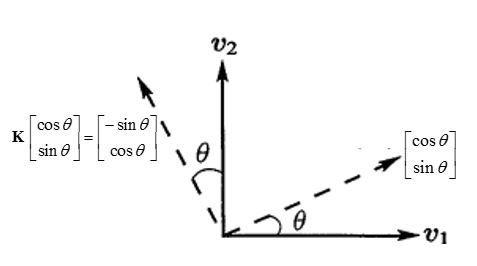
\includegraphics[width=10cm]{week6/rotation}
\caption{Rotate a vector by $90\degree$.}
\end{figure}
This rotation matrix exists eigenvector and eigenvalue, which means $\exists\bm v\ne\bm 0$ and $\lambda$ s.t. \[\bm K\bm v=\lambda\bm v.\] 
However, this equation means this rotaion matrix doesn't change the direction of $\bm v$. But in geometric meaning it rotates vector $\bm v$ by $90\degree$. Why? This phenomenon will not happen unless we go to imaginary eigenvectors. Let's compute eigenvalues and eigenvectors for $\bm K$ first:
\[
P_{\bm K}(\lambda)=\begin{vmatrix}
\lambda&1\\-1&\lambda\end{vmatrix}
=\lambda^2+1
\implies
\lambda_1=i,\quad\lambda_2=-i.
\]
\begin{align*}
(\lambda_1\bm I-\bm K)\bm x&=\begin{pmatrix}
i&1\\-1&i
\end{pmatrix}\begin{pmatrix}
x_1\\x_2
\end{pmatrix}=\bm 0\implies\bm x=\alpha\begin{pmatrix}
1\\-i
\end{pmatrix}.\\
(\lambda_2\bm I-\bm K)\bm x&=\begin{pmatrix}
-i&1\\-1&-i
\end{pmatrix}\begin{pmatrix}
x_1\\x_2
\end{pmatrix}=\bm 0\implies\bm x=\beta\begin{pmatrix}
1\\i
\end{pmatrix}.
\end{align*}
Moverover, we can do similar transformation for $\bm K$:
\[
\bm D=\bm S^{-1}\bm K\bm S=\begin{pmatrix}
i&\\&-i
\end{pmatrix}\qquad\text{where $\bm S=\begin{bmatrix}
1&1\\-i&i
\end{bmatrix}$.}
\]
\end{example}
\begin{remark}
For motion in vector space, eigenvalues are ``speed''
 and eigenvectors are ``directions'' under basis $\bm S=\begin{bmatrix}
\bm x_1&\bm x_2&\dots&\bm x_n
\end{bmatrix}$.
\[
\bm v=c_1\bm x_1+\dots+c_n\bm x_n
\xLongrightarrow{\text{postmultiply $\bm A$}}\bm{Av}=c_1\lambda_1\bm x_1+\dots+c_n\lambda_n\bm x_n.
\]
\[
\begin{pmatrix}
c_1&\dots&c_n
\end{pmatrix}
\xLongrightarrow{\text{rightmultiply $\bm D=\diag(\lambda_1,\dots,\lambda_n)$}}
\begin{pmatrix}c_1\lambda_1&\dots&c_n\lambda_n
\end{pmatrix}.
\]
\end{remark}
\subsection{Complex Numbers}
Even when the matrix is real, its eigenvalues of this matrix may be complex numbers. Example: A 2 by 2
rotation matrix has no real eigenvectors. It rotates a vector by $90\degree$. But it has complex eigenvalues $i$ and $-i$.
\begin{definition}[Complex Numbers]
A cpmplex number $\bm x\in\mathbb{C}$ could be written as $\bm x=a+bi$, where $i^2=-1$.\\
Its \emph{complex conjugate} is defined as $\bm{\bar x}=a-bi$.\\
Its \emph{modulus} is defined as $|\bm x|=\sqrt{a^2+b^2}=\sqrt{\bm x\bm{\bar x}}.$
\end{definition}
\begin{figure}[H]
\centering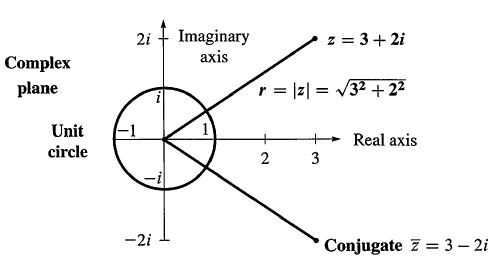
\includegraphics{week6/complex}
\caption{The number $z=a+bi$ corrsponds to the vector 
$(a,b)$.}
\end{figure}
\subsection{Complex Vectors}
\begin{definition}[Length (norm) for complex]
For $z=\begin{bmatrix}
z_1\\z_2\\\vdots\\z_n
\end{bmatrix}\in\mathbb{C}^n$, its \emph{length (norm)}
 is defined as
\[
\|z\|=\sqrt{|z_1|^2+|z_2|^2+\dots+|z_n|^2}=\sqrt{\inp{z}{z}}=\sqrt{z_1\bar z_1+z_2\bar z_2+\dots+z_n\bar z_n}.
\]
\end{definition}
Before we introduce the definition of inner product for complex, let's introduce the \textit{Hermitian} of a vector in $\mathbb{C}^n$:
\begin{definition}[Hermitian]
The hermitian of a vector in $\mathbb{C}^n$ is its \textit{conjugate transpose}.
\[
\bm z=\begin{bmatrix}
z_1\\\vdots\\z_n
\end{bmatrix}\qquad
\bm z\Her=\bm{\bar z}\trans=\begin{bmatrix}
\bar z_1&\dots&\bar z_n
\end{bmatrix}.
\]
\end{definition}
\newpage
\begin{definition}[Inner product]
The inner product of real or complex vectors $\bm z$ and $\bm w$ is $\bm w\Her\bm z$, which is defined as
\[
\inp{\bm z}{\bm w}=\bm w\Her\bm z=\begin{bmatrix}
\bm{\bar w_1}&\dots&\bm{\bar w_n}
\end{bmatrix}\begin{bmatrix}
\bm{z_1}\\\vdots\\\bm{z_n}
\end{bmatrix}=\bm{\bar w_1}\bm{z_1}+\dots+\bm{\bar w_n}\bm{z_n}.
\]
\end{definition}
\begin{remark}
Note that with complex vectors, $\bm w\Her\bm z$ is different from $\bm z\Her\bm w$. \emph{The order of the vectors is now important!} In fact, $\bm z\Her\bm w=\bm{\bar z_1}\bm{w_1}+\dots+\bm{\bar z_n}\bm{w_n}$ is the complex conjugate of $\bm w\Her\bm z$.
\end{remark}
\begin{definition}[Orthogonal]
The two vectors of real or complex are \textit{orthogonal} if their \emph{inner product} is zero.
\[
\bm z\perp\bm w\implies
\inp{\bm z}{\bm w}=\bm w\Her\bm z=0
\]
\end{definition}
\begin{example}\qquad\\
Given $\bm z=\begin{pmatrix}
1\\i
\end{pmatrix}, \bm w=\begin{pmatrix}
-i\\1
\end{pmatrix}$.\\
Although we have $\bm z\trans\bm w=0$, the two vectors are not perpendicular.\\ This is because $\inp{\bm z}{\bm w}=\bm w\Her\bm z=\begin{bmatrix}
i&1
\end{bmatrix}\begin{bmatrix}
1\\i
\end{bmatrix}=2i\ne0.$
\end{example}
\begin{example}
The inner product of $\bm u=\begin{bmatrix}
1\\i
\end{bmatrix}$ with $\bm v=\begin{bmatrix}
i\\1
\end{bmatrix}$ is $\begin{bmatrix}
-i&1
\end{bmatrix}\begin{bmatrix}
1\\i
\end{bmatrix}=0.$\\
Although those vectors $(1,i)$ and $(i,1)$ don't look perpendicular, actually they are! \emph{A zero inner product still means vectors are orthogonal.}
\end{example}
\begin{proposition}[Conjugate symmetry]\qquad\\
For two vectors $\bm z$ and $\bm w\in\mathbb{C}^{n}$, we have $\overline{\inp{\bm z}{\bm w}}=\inp{\bm w}{\bm z}.$
\end{proposition}
\begin{proof}[Verify:]
\begin{gather*}
\inp{\bm z}{\bm w}=\bm w\Her\bm z=\bm{\bar w}\trans\bm z
=\bm{\bar w_1}\bm{z_1}+\dots+\bm{\bar w_n}\bm{z_n}
\\
\inp{\bm w}{\bm z}=\bm z\Her\bm w=\bm{\bar z}\trans\bm w
=\bm{\bar z_1}\bm{w_1}+\dots+\bm{\bar z_n}\bm{w_n}
\end{gather*}
And since we have $\overline{\bm w\bm v}=\bm{\bar w}\bm{\bar v}$ and $\overline{\bm w+\bm v}=\bm{\bar w}+\bm{\bar v}$, it's easy to find that
\[
\overline{\bm{\bar w_1}\bm{z_1}+\dots+\bm{\bar w_n}\bm{z_n}}
=\bm{w_1}\bm{\bar z_1}+\dots+\bm{w_n}\bm{\bar z_n}.
=\bm{\bar z_1}\bm{w_1}+\dots+\bm{\bar z_n}\bm{w_n}.
\]
Hence $\overline{\inp{\bm z}{\bm w}}=\inp{\bm w}{\bm z}.$
\end{proof}
\begin{proposition}[Sesquilinear]\qquad\\
For two vectors $\bm z$ and $\bm w\in\mathbb{C}^{n}$, we have
\begin{gather}
\inp{\alpha\bm z}{\bm w}=\alpha\inp{\bm z}{\bm w}\\
\inp{\bm z}{\beta\bm w}=\bar\beta\inp{\bm z}{\bm w}\label{eq:16.2}
\end{gather}
for scalars $\alpha$ and $\beta$.
\end{proposition}
\begin{proof}[Verify:]
\begin{align*}
\inp{\alpha\bm z}{\bm w}&=\bm w\Her(\alpha\bm z)\\&=\alpha(\bm w\Her\bm z)\\&=\alpha\inp{\bm z}{\bm w}.
\end{align*}
For equation (\ref{eq:16.2}), due to the conjugate symmetry, we derive
\[
\inp{\bm z}{\beta\bm w}=\overline{\inp{\beta\bm w}{\bm z}}
\]
Since $\inp{\beta\bm w}{\bm z}=\beta\inp{\bm w}{\bm z}=\beta\overline{\inp{\bm z}{\bm w}}$, we obtain
\[
\inp{\bm z}{\beta\bm w}=\overline{\beta\overline{\inp{\bm z}{\bm w}}}=\bar\beta\inp{\bm z}{\bm w}.
\]
\end{proof}
\subsubsection{Hermitian of matrix}
The Hermitian of a matrix $\bm A$ is given by
\[
\bm A\Her:=\bar{\bm A}\trans
\]
And the rules for hermitian usually comes frim transpose. For example, the hermitian has the property
\[
(\bm A\bm B)\Her=\bm B\Her\bm A\Her.
\]
\begin{center}
\begin{tabular}{cU}
\hline
  $\mathbb{R}^n$  & $\mathbb{C}^n$ \\
  
$\inp{\bm x}{\bm y}=\bm x\trans\bm y$ &  $\inp{\bm z}{\bm w}=\bm w\Her\bm z$\\

$\bm x\trans\bm y=\bm y\trans\bm x$  & $\bm z\Her\bm w=\overline{\bm w\Her\bm z}$\\

$\|\bm x\|^2=\bm x\trans\bm x$   &   $\|\bm z\|^2=\bm z\Her\bm z$\\

$\bm x\perp\bm y\Longleftrightarrow \bm x\trans\bm y=0$&
$\bm z\perp\bm w\Longleftrightarrow \bm w\Her\bm z=0$\\
\hline
\end{tabular}
\end{center}
\begin{remark}
\textit{What aspects of eigenvalues/eigenvectors are not nice?}\\
\begin{itemize}
\item
Some matrix are \textit{non-diagonalizable}. (or equivalently, eigenvectors don't form a basis.)
\item
Eigenvalues can be \textit{complex}.
\end{itemize}
We may ask, what matrix has all real eigenvalues? Let's focus on \textit{real} matrix first. For real symmetric matrix, its eigenvalues are all real!
\end{remark}
You should remember the proposition below carefully, they are very important.
\begin{proposition}\label{real_symmetric}
For a \textit{real symmetric} matrix $\bm A$, 
\begin{itemize}
\item
All eigenvalues are real numbers.
\item
Its eigenvectors corresponding to distinct eigenvalues are orthogonal.
\item
$\bm A$ is diagonalizable. More general, all eigenvectors of $\bm A$ are orthogonal!
\end{itemize}
\end{proposition}
Before the proof, let's introduce a useful formula: $\inp{\bm{Ax}}{\bm y}=\inp{\bm x}{\bm A\Her\bm y}$.\\
\[
\textit{Verify: }\inp{\bm{Ax}}{\bm y}=\bm y\Her\bm{Ax}=(\bm A\Her\bm y)\Her\bm x=\inp{\bm x}{\bm A\Her\bm y}
\]
\begin{proof}
\begin{itemize}
\item
For the first part, suppose $\bm x$ is any eigenvectors of $\bm A$ corresponding to eigenvalue $\lambda$. Then we obtain
\[
\inp{\bm{Ax}}{\bm x}=\inp{\bm x}{\bm A\Her\bm x}
\]
\begin{itemize}
\item
For the LHS, $\inp{\bm{Ax}}{\bm x}=\inp{\lambda\bm x}{\bm x}=\lambda\inp{\bm x}{\bm x}$.
\item
For the RHS, Since $\bm A$ is a real symmetric matrix, we have $\bm A\Her=\bar{\bm A}\trans=\bm A\trans=\bm A$.\\ Hence $\inp{\bm x}{\bm A\Her\bm x}=\inp{\bm x}{\bm{Ax}}$. Moreover, $\inp{\bm x}{\bm{Ax}}=\inp{\bm x}{\lambda\bm x}=\bar\lambda\inp{\bm x}{\bm x}$.\\ So we have $\inp{\bm x}{\bm A\Her\bm x}=\bar\lambda\inp{\bm x}{\bm x}.$
\end{itemize}
Finally we have $\lambda\inp{\bm x}{\bm x}=\inp{\bm{Ax}}{\bm x}=\inp{\bm x}{\bm A\Her\bm x}=\bar\lambda\inp{\bm x}{\bm x}.$\\
Since $\bm x\ne\bm 0$, $\inp{\bm x}{\bm x}\ne0.$ Hence $\lambda=\bar\lambda$. So $\lambda$ is real.
\item
For the second part, suppose $\bm x_1$ and $\bm x_2$ are two eigenvectors corresponding to two \emph{distinct} eigenvalues $\lambda_1$ and $\lambda_2$ respectively. Our goal is to show $\bm x_1\perp\bm x_2$. We find that
\[
\inp{\bm A\bm x_1}{\bm x_2}=\inp{\bm x_1}{\bm A\Her\bm x_2}
\]
\begin{itemize}
\item
For LHS, $\inp{\bm A\bm x_1}{\bm x_2}=\inp{\lambda_1\bm x_1}{\bm x_2}=\lambda_1\inp{\bm x_1}{\bm x_2}$.
\item
For RHS, $\inp{\bm x_1}{\bm A\Her\bm x_2}=\inp{\bm x_1}{\bm A\bm x_2}=\inp{\bm x_1}{\lambda_2\bm x_2}=\bar\lambda_2\inp{\bm x_1}{\bm x_2}$. Since we have shown that all eigenvalues are real for $\bm A$, we obtain $\bar\lambda=\lambda$.\\
Hence $\inp{\bm x_1}{\bm A\Her\bm x_2}=\lambda_2\inp{\bm x_1}{\bm x_2}.$
\end{itemize}
Hence $\lambda_1\inp{\bm x_1}{\bm x_2}=\inp{\bm A\bm x_1}{\bm x_2}=\inp{\bm x_1}{\bm A\Her\bm x_2}=\lambda_2\inp{\bm x_1}{\bm x_2}.$\\ Since $\lambda_1\ne\lambda_2$, we obtain $\inp{\bm x_1}{\bm x_2}=0.$ That is to say, $\bm x_1\perp\bm x_2.$
\item
The proof for the third part is not required.
\end{itemize}
\end{proof}
\subsection{Spectral Theorem}
We state a theorem without proving it:
\begin{theorem}[Spectral Theorem]
Any real symmetric matrix $\bm A$ has the factorization \begin{equation}
\bm A=\bm Q\Lambda\bm Q\trans,
\end{equation} where $\Lambda\in\mathbb{R}^{n\x n}$ is diagonal matrix, $\bm Q\in\mathbb{R}^{n\x n}$ is orthogonal matrix.
\end{theorem}
\begin{proof}
From proposition (\ref{real_symmetric}) we know that $\bm A$ is \textit{diagonalizable}, which means there exists invertible matrix $\bm Q$ and diagonal matrix $\Lambda$ such that
\[
\bm A=\bm Q\Lambda\bm Q^{-1}
\]
Then we know that all eigenvalues of $\bm A$ are real numbers, so $\Lambda$ is a real matrix.\\
Since all eigenvectors $\bm x_1,\dots,\bm x_n$ are orthogonal, matrix $\bm Q=\begin{bmatrix}
\bm x_1&\dots&\bm x_n
\end{bmatrix}$ is orthogonal matrix.
\end{proof}
\begin{remark}
$\bm A=\bm Q\Lambda\bm Q\trans=\bm Q\Lambda\bm Q^{-1}$. So $\bm A$ could be diagonalized by an orthogonal matrix.\\
If we let $\bm Q=\begin{bmatrix}
q_1&\dots&q_n
\end{bmatrix}$, $\Lambda=\diag(\lambda_1,\dots,\lambda_n)$, then $\bm A$ could be written as:
\[
\bm A=\bm Q\Lambda\bm Q\trans=
\begin{bmatrix}
q_1&\dots&q_n
\end{bmatrix}\begin{bmatrix}
\lambda_1&&\\&\ddots&\\&&\lambda_n
\end{bmatrix}\begin{bmatrix}
q_1\trans\\\vdots\\q_n\trans
\end{bmatrix}
\]
Or equivalently,
\begin{equation}
\bm A=\lambda_1q_1q_1\trans+\lambda_2q_2q_2\trans+\dots+\lambda_nq_nq_n\trans
\end{equation}
Note that for each term $q_iq_i\trans$ is the \emph{projection matrix} to $q_i$. Hence this theorm says that a real symmetric matrix is a combination of projection matrices.
\end{remark}
\newpage
\begin{example}\qquad\\
If we write $\bm A$ as combination of projection matrix, we can have a deep understanding for $\bm{Ax}$:
\[
\bm A=\sum_{j=1}^{n}\lambda_jq_jq_j\trans
\implies
\bm{Ax}=\sum_{j=1}^{n}\lambda_jq_jq_j\trans\bm x=
\sum_{j=1}^{n}\lambda_j(q_jq_j\trans\bm x).
\]
If we set $n=2$, it's clear to find that
\[
\bm x=c_1q_1+c_2q_2\implies
\bm{Ax}=\lambda_1c_1q_1+\lambda_2c_2q_2
\]
Showing in graph, we have
\begin{figure}[H]
\centering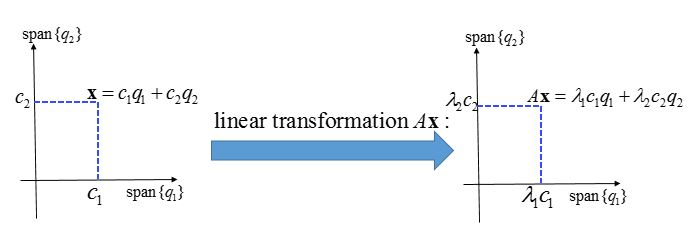
\includegraphics[width=12cm]{week6/spec}
\caption{Linear transformation of $\bm A$.}
\end{figure}
\end{example}
The formula $\bm A=\sum_{j=1}^{n}\lambda_jq_jq_j\trans$ or $\bm A=\bm Q\Lambda\bm Q\trans$ are called \emph{eigendecomposition} or \emph{eigenvalue decomposition}.\\
And sometimes $\{\lambda_1,\dots,\lambda_n\}$ are called \emph{spectum} of $\bm A$.\\
Also, we can extend our result from real symmetric matrix into complex:
\subsection{Hermitian matrix}
\begin{definition}[Hermitian matrix]
A matrix $\bm M\in\mathbb{C}^{n\x n}$ is said to be \emph{Hermitian} if $\bm M=\bm M\Her$.
\end{definition}
\emph{Example: }$\bm M=\begin{bmatrix}
3&2-i\\2+i&4
\end{bmatrix}$ is Hermitian matrix since $\bm M=\bm M\Her$.\\
If $\bm M$ is a real matrix, then $\bm M=\bm M\Her\Longleftrightarrow\bm M=\bm M\trans$. So if the real matrix is Hermitian matrix, that is to say it is real symmetric matrix.\\
Hermitian matrix has many interesting properties:
\begin{proposition}
If $\bm M=\bm M\Her$, then $\bm x\Her\bm M\bm x\in\mathbb{R}$ for any complex vectors $\bm x$.
\end{proposition}
\begin{proof}
We set $\alpha:=\bm x\Her\bm M\bm x$. Since $\alpha$ is a number (easy to check), we obtain $\alpha\trans=\alpha.$\\
Thus $\bar\alpha=\alpha\Her=(\bm x\Her\bm M\bm x)\Her=\bm x\Her\bm M\bm x=\alpha.$\\
Hence $\alpha$ is real.
\end{proof}
\begin{proposition}
If $\bm M=\bm M\Her$, then $\inp{\bm x}{\bm{My}}=\inp{\bm{Mx}}{\bm y}.$
\end{proposition}
\begin{proof}
By definition,
\[
\inp{\bm x}{\bm{My}}=(\bm{My})\Her\bm x=\bm y\Her\bm M\Her\bm x=\bm y\Her\bm M\bm x=\inp{\bm{Mx}}{\bm y}.
\]
\end{proof}
And we have general orthogonal matrices for complex matrices:
\begin{definition}[Unitary]
A unitary matrix is a complex matrix that has \emph{orthonormal columns}. In other words, $\bm U$ is unitary if $\bm U\Her\bm U=\bm I.$
\end{definition}
And the spectral theorm can also apply for Hermitian matrix:
\begin{theorem}
Any Hermitian matrix $\bm M$ can be factorized into
\[
\bm M=\bm U\Lambda\bm U\Her
\]
where $\Lambda$ is a real diagonal matrix, $\bm U$ is a complex unitary matrix.
\end{theorem}
\begin{remark}
What good points does Hermitian matrix have?
\begin{itemize}
\item
It is diagonalizable.
\item
Its eigenvectors form orthogonal basis.
\item
Its eigenvalues are all real.
\end{itemize}
\end{remark}
\section{Assignment Seven}\index{Assignment_Seven}
\begin{enumerate}
\item
Here is a wrong ``proof'' that the \textit{eigenvalues of all real matrices are real}:
\[
\bm{Ax}=\lambda\bm x\text{ gives }\bm x\trans\bm A\bm x=\lambda\bm x\trans\bm x
\implies
\lambda=\frac{\bm x\trans\bm A\bm x}{\bm x\trans\bm x}\in\mathbb{R}.
\]
Find the flaw in this reasoning: a hidden assumption that is not justified.
\item
Let $\bm A$ be an $n\x n$ matrix and let $\lambda$ be an eigenvalue of $\bm A$ whose eigenspace has
dimension $k$, where $1<k<n$. Any basis $\{\bm x_1,\dots,\bm x_k\}$ for the eigenspace can be
extended to a basis $\{\bm x_1,\dots,\bm x_n\}$ for $\mathbb{R}^n$. Let $\bm X=\begin{bmatrix}
\bm x_1&\cdots&\bm x_n
\end{bmatrix}\trans$ and $\bm B=\bm X^{-1}\bm A\bm X.$
\begin{enumerate}
\item
Show that $\bm B$ is of the form
\[
\begin{bmatrix}
\lambda\bm I&\bm B_{12}\\
\bm0&\bm B_{22}
\end{bmatrix}
\]
where $\bm I$ is the $k\x k$ identity matrix
\item
Show that $\lambda$ is an eigenvalue of $\bm A$ with multiplicity at least $k$.
\end{enumerate}
\item
Let $\bm x,\bm y$ be nonzero vectors in $\mathbb{R}^n$, $n\ge2$, and let $\bm A=\bm x\bm y\trans$. Show that
\begin{enumerate}
\item
$\lambda=0$ is an eigenvalue of $\bm A$ with $n-1$ linearly independent eigenvectors. Moreover, due to the conclusion of question 2, $0$ is an eigenvalue of $\bm A$ with multiplicity at least $n-1$.
\item
The remaining eigenvalue of $\bm A$ is
\[
\lambda_n=\trace(\bm A)=\bm x\trans\bm y
\]
and $\bm x$ is an eigenvector belonging to $\lambda_n.$
\item
If $\lambda_n=\bm x\trans\bm y\ne0,$ then $\bm A$ is \textit{diagonalizable.}
\end{enumerate}
\item
Suppose an $n\x n$ matrix $\bm A$ has $n$ distinct eigenvalues $\lambda_1,\dots,\lambda_n$. Consider the matrix $\bm B=(\bm A-\lambda_1\bm I)\dots(\bm A-\lambda_n\bm I)$. Prove that $\bm B$ must be a \textit{zero matrix}.\\
\textit{Hint:} How to do eigendecomposition for $\bm A-\lambda_i\bm I$?
\item
Let $\bm A$ and $\bm B$ be $n\x n$ matrices. Show that
\begin{enumerate}
\item
If $\lambda$ is a \emph{nonzero} eigenvalue of $\bm{AB}$, then it is also an eigenvalue of $\bm{BA}$.
\item
If $\lambda=0$ is an eigenvalue of $\bm{AB}$, then $\lambda=0$ is also an eigenvalue of $\bm{BA}$.
\end{enumerate}
\item
\begin{enumerate}
\item
The sequence $a_k$ is defined as
\[
a_0=4,a_1=5,a_{k+1}=3a_k-2a_{k-1},k=1,2,\dots
\]
What is the \textit{general formula} for $a_k$?
\item
The sequence $b_k$ is defined as
\[
b_0=\alpha,b_1=\beta,b_{k+1}=4b_k-4b_{k-1},k=1,2,\dots
\]
What is the \textit{general formula} for $b_k$?\\
\textit{Hint:} Prove the corresponding matrix is similar to
\[
\begin{bmatrix}
2&1\\0&2
\end{bmatrix}.
\]
In order to compute
\[
\begin{bmatrix}
2&1\\0&2
\end{bmatrix}^k,
\]
you need to use the fact that
\[
\text{Given sequence }p_{k+1}=2p_{k}+2^k
\implies
p_k=(p_0+\frac{k}{2})\times2^k.
\]
\end{enumerate}
\item
State and justify whether the following three statements are True or False:
\begin{enumerate}
\item
If $\bm A$ is \textit{real symmetric} matrix, then any 2 linearly independent eigenvectors of $\bm A$ are perpendicular.
\item
Any $n$ by $n$ complex matrix with $n$ real eigenvalues and $n$ orthonormal eigenvectors
is a \textit{Hermitian matrix}.
\item
If $\bm A$ is diagonalizable. then $e^{\bm A}$ is diagonalizable.\\
(We define $e^{\bm A}=\bm I+\bm A+\frac{1}{2!}\bm A^2+\dots$)
\item
If $\bm A$ is Hermitian and $\bm A$ is invertible, then $\bm A^{-1}$ is also Hermitian.
\end{enumerate}
\item
\begin{enumerate}
\item
For a complex $\bm A$, is the left nullspace $N(\bm A\trans)$ orthogonal to $C(\bm A)$ under the old
unconjugated inner product $\bm x\trans\bm y$ or new conjugated inner product $\bm x\Her\bm y$? What about
$N(\bm A\Her)$ and $C(\bm A)$?
\item
For a real vector subspace $V$, the intersection of $V$ and $V^{\perp}$ is only the single point $\{\bm 0\}$. Now suppose $V$ is a complex vector subspace. If we define $V^{\perp}$ as the set of vector $\bm x$ with $\bm x\trans\bm v=0$ for all $\bm v\in V$. Give an example of a $V$ that intersects $V^{\perp}$ at a nonzero vector. What about if we use $\bm x\Her\bm v=0$? Does $V$ ever intersect $V^{\perp}$ at a nonzero vector using the conjugated definition of orthogonality?
\end{enumerate}
\end{enumerate}
%\include{week7/Lecture_1}
\chapterimage{Tuesdayimage}% Chapter heading image

\chapter{Week7}

\section{Tuesday}\index{week7_Tuesday_lecture}\subsection{Quadratic form}
The graphs of the following equations are easy to plot:
\begin{gather}
x^2+y^2=1\label{eq:17.1}\implies\text{ Circle}.\\
\frac{x^2}{2}+\frac{y^2}{5}=1\label{eq:17.2}\implies\text{ Elipse}.\\
\frac{x^2}{2}-\frac{y^2}{5}=1\label{eq:17.3}\implies\text{ Hyperbola}.\\
\left.\begin{align*}
x^2&=\alpha y\\
y^2&=\alpha x
\end{align*}\right\}\implies\text{ Parabola}.
\end{gather}
\begin{figure}[H]
\centering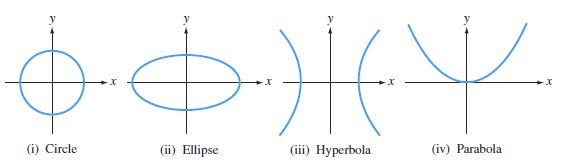
\includegraphics{week7/shape}
\caption{graph for quadratic form equations of two variables}
\end{figure}
The equations $(\ref{eq:17.1})-(\ref{eq:17.3})$ is the \textit{quadratic form equations of two variables}. Now we give the general form for quadratic equations:
\begin{definition}[Quadratic form]
The formula of \emph{quadratic form} is given by
\[
\bm x\trans\bm A\bm x
\]
where $\bm A$ is $n\x n$ matrix, $\bm x\in\mathbb{R}^{n}$.\\
Moreover, sometimes we write $\bm x\trans\bm A\bm x$ as:
\[
\bm x\trans\bm A\bm x=\sum_{i,j=1}^{n}x_ix_ja_{ij}
\]
where $x_i$ is the $i$th entry of $\bm x$ and $a_{ij}$ are $(i,j)$th entry of $\bm A$.
\end{definition}
Moverover, we say an equation is the \emph{conic section of quadratic form} if it can be written as
\[
\bm x\trans\bm A\bm x=1.
\]
\begin{itemize}
\item
Note that $\bm x\trans\bm A\bm x=\bm x\trans\bm A\trans\bm x$. Why?\\ If we take the transpose of $\bm x\trans\bm A\bm x$, since it is a number, so we obtain
\[
(\bm x\trans\bm A\bm x)\trans=\bm x\trans\bm A\bm x.
\]
Since $(\bm x\trans\bm A\bm x)\trans=\bm x\trans\bm A\trans\bm x$, finally we derive 
\[
\bm x\trans\bm A\bm x=\bm x\trans\bm A\trans\bm x.
\]
\item
Hence given any matrix $\bm A$, we always have
\begin{align*}
\bm x\trans\left(\frac{\bm A+\bm A\trans}{2}\right)\bm x&=\frac{1}{2}\bm x\trans\bm A\bm x+\frac{1}{2}\bm x\trans\bm A\trans\bm x\\&=\frac{1}{2}\bm x\trans\bm A\bm x+\frac{1}{2}\bm x\trans\bm A\bm x\\&=\bm x\trans\bm A\bm x.
\end{align*}
Note that $\left(\frac{\bm A+\bm A\trans}{2}\right)$ is \textit{symmetric}! Hence given any $\bm A$, if we want to study its quadratic form, we can always convert this matrix into symmetric matrix.\\
\end{itemize}
Hence without loss of generality, we assume $\bm A=\bm A\trans$ during the section of quadratic form.
\begin{example}\qquad\\
Given the equation $3x^2+2xy+3y^2=1$, how we transform it into the conic section of quadratic form? And how can we determine its shape in view of matirx?\\
Actually, It can be written as
\begin{equation}
\begin{pmatrix}
x&y
\end{pmatrix}\begin{pmatrix}
3&1\\1&3
\end{pmatrix}\begin{pmatrix}
x\\y
\end{pmatrix}=1.\qquad\qquad\text{\emph{conic section of quadratic form.}}
\label{conic_section}
\end{equation}
And we define $\bm A=\begin{pmatrix}
3&1\\1&3
\end{pmatrix}.$ If we do the eigendecomposition for $\bm A$, we obtain
\[
\bm A=\bm Q\Lambda\bm Q\trans
\]
where $\Lambda=\begin{pmatrix}
\lambda_1&\\&\lambda_2
\end{pmatrix}$, $\bm Q=\begin{bmatrix}
\bm x_1&\bm x_2
\end{bmatrix}$. $\bm x_1$,$\bm x_2$ is the eigenvectors of $\bm A$ corresponding to eigenvalues $\lambda_1$,$\lambda_2$ respectively.\\
Thus we convert equation (\ref{conic_section}) into
\[
\begin{pmatrix}
x&y
\end{pmatrix}\bm Q\Lambda\bm Q\trans\begin{pmatrix}
x\\y
\end{pmatrix}=1
\implies
\tilde{\bm x}\trans\Lambda\tilde{\bm x}=1.
\]
where $\tilde{\bm x}=\bm Q\trans\begin{pmatrix}
x\\y
\end{pmatrix}=\begin{pmatrix}
\tilde x_1\\\tilde x_2
\end{pmatrix}$.\\
Then how to determine the shape of this equation? We just do matrix multiplication to obtain:
\[
\lambda_1\tilde x_1^2+\lambda_2\tilde x_2^2=1.
\]
After computation, we find $\lambda_1=4,\lambda_2=2$. Hence this equation is a \emph{elipse.}
\end{example}
\begin{remark}
\subsubsection{Matrix Calculus}
Now we recall how to compute derivative for matrix:
\begin{itemize}
\item
$\frac{\partial(f\trans g)}{\partial x}=\frac{\partial f(x)}{\partial x}g(x)+\frac{\partial g(x)}{\partial x}f(x)$
\end{itemize}
Example:
\begin{itemize}
\item
$\frac{\partial(a\trans \bm x)}{\partial \bm x}=a$
\item
$\frac{\partial(a\trans \bm A\bm x)}{\partial \bm x}=\frac{\partial((\bm A\trans a)\trans\bm x)}{\partial \bm x}=\bm A\trans a$
\item
$\frac{\partial(\bm A\bm x)}{\partial \bm x}=\bm A\trans$
\item
$\frac{\partial(\bm x\trans\bm A\bm x)}{\partial \bm x}=\bm A\bm x+\bm A\trans\bm x$
\end{itemize}
\end{remark}
\begin{example}\qquad\\
Given $f(\bm x)=\frac{1}{2}\bm x\trans\bm A\bm x+\bm b\trans\bm x$. We want to do the optimization:
\[
\min_{\bm x\in\mathbb{R}^{n}}f(\bm x)
\]
How to find the optimal solution? The direct idea is to take the first order derivative:
\begin{align*}
\frac{\partial f}{\partial \bm x}&=\frac{1}{2}\frac{\partial(\bm x\trans\bm A\bm x)}{\partial \bm x}+\frac{\partial(\bm b\trans\bm x)}{\bm x}\\
&=\frac{1}{2}(\bm{Ax}+\bm A\trans\bm x)+\bm b.
\end{align*}
Since $\bm A$ is symmetric, we obtain
\[
\frac{\partial f}{\partial \bm x}=\bm{Ax}+\bm b.
\]
If $\bm x^{*}$ is an optimal solution, then it must satisfy:
\[
\bigtriangledown f(\bm x^{*})=\frac{\partial f(\bm x^{*})}{\partial \bm x}=\bm 0\implies
\bm A\bm x^{*}+\bm b=\bm 0.
\]
There may follow these cases:
\begin{itemize}
\item
If equation $\bm{Ax}+\bm b=\bm 0$ has no solution, then $f(\bm x)$ is unbounded.\\
This statement is remained to be proved.
\item
If equation $\bm{Ax}+\bm b=\bm 0$ has a solution $\bm x^{*}$, it doesn't mean $\bm x^{*}$ is an optimal solution. (Note that the reverse is true.)\\
Let's raise a counterexample: if we set
\[
\bm A=\begin{bmatrix}
1&0\\0&-1
\end{bmatrix},\qquad\bm b=\bm 0,\qquad\bm x=\begin{pmatrix}
x_1\\x_2
\end{pmatrix},
\]
then $f(\bm x)=\frac{1}{2}(x_1^2-x_2^2)$.\\
One solution to $\bm{Ax}+\bm b=\bm 0$ is $\bm x^*=\begin{pmatrix}
0\\0
\end{pmatrix}$. Obviously, $\bm x^{*}$ is not a optimal solution. Intutively, if we let $x_1=0,x_2\rightarrow\infty$, then $f(\bm x)\rightarrow-\infty$!
\end{itemize}
\end{example}
\subsubsection{Second optimality condition}
If $\bm x^{*}$ is a optimal solution to $f(\bm x)$, what else condition should $\bm x^{*}$ satisfy?\\ Let's take $f(\bm x)=\frac{1}{2}\bm x\trans\bm A\bm x+\bm b\trans\bm x$ as an example, we want to find $\bm x^{*}$ s.t. $\min f(\bm x)=f(\bm x^{*})$.\\
Firstly, we convert $f(\bm x)$ into its \textit{taylor expansion}:
\[
f(\bm x)=f(\bm x^{*})+\inp{\bigtriangledown f(\bm x^*)}{\bm x-\bm x^*}+\frac{1}{2}(\bm x-\bm x^*)\trans\bigtriangledown^2f(\bm x^*)(\bm x-\bm x^*).
\]
Note that $\bigtriangledown^2f(\bm x^*)$ is the Hessian matrix of $f(\bm x^*)$, which is defined as \[\bigtriangledown^2f(\bm x^*):=\begin{bmatrix}
\frac{\partial^2 f(\bm x^*)}{\partial x_{i}\partial x_{j}}
\end{bmatrix}=\bigtriangledown(\bigtriangledown f(\bm x^*)).\]
Firstly we compute $\bigtriangledown f(\bm x)$ and $\bigtriangledown^2 f(\bm x)$:
\begin{align*}
\bigtriangledown f(\bm x)&=\frac{1}{2}(\bm{Ax}+\bm A\trans\bm x)+\bm b.\\
\bigtriangledown^2 f(\bm x)&=\bigtriangledown\left[\frac{1}{2}(\bm{Ax}+\bm A\trans\bm x)+\bm b\right]=\frac{1}{2}\bigtriangledown(\bm{Ax})+\frac{1}{2}\bigtriangledown(\bm A\trans\bm x)
=\frac{1}{2}(\bm A+\bm A\trans).
\end{align*}
If we assume $\bm A$ is \emph{symmetric}, then we have $\bigtriangledown f(\bm x)=(\bm A+\bm A\trans)\bm x+\bm b$ and $\bigtriangledown^2 f(\bm x)=\bm A$.\\
Since the optimal solution $\bm x^*$ must satisfy $\bigtriangledown f(\bm x^*)=\bm 0$, we deive \[\inp{\bigtriangledown f(\bm x^*)}{\bm x-\bm x^*}=0.
\implies
f(\bm x)=f(\bm x^{*})+\frac{1}{2}(\bm x-\bm x^*)\trans\bigtriangledown^2f(\bm x^*)(\bm x-\bm x^*).
\]
Hence $f(\bm x)-f(\bm x^{*})=\frac{1}{2}(\bm x-\bm x^*)\trans\bm A(\bm x-\bm x^*).$\\
Since $\bm x^*$ is optimal that minimize $f(\bm x)$, $LHS=f(\bm x)-f(\bm x^*)\ge0$.
\[
\implies 
\frac{1}{2}(\bm x-\bm x^*)\trans\bm A(\bm x-\bm x^*)\ge0
\]
Or equivalently,
\[
(\bm x-\bm x^*)\trans\bm A(\bm x-\bm x^*)\ge0\text{ for $\forall\bm x$.}
\Longleftrightarrow
\bm x\trans\bm A\bm x\ge0 \text{ for $\forall\bm x$.}
\]
Our conclusion is that if there exists a optimal solution for $f(\bm x)$, then the matrix $\bm A$ should satisfy $\bm x\trans\bm A\bm x\ge0$ for $\forall\bm x.$ We have a specific name for such $\bm A$.
\subsection{Positive Definite Matrices}
\begin{definition}[Positive-definite]\qquad\\
\begin{itemize}
\item
Matrix $\bm A$ is \textit{positive-semidefinite} (PSD) if $\bm x\trans\bm A\bm x\ge0$ for $\forall\bm x.$ And we denote it as $\bm A\succeq0.$
\item
Matrix $\bm A$ is \textit{positive-definite} (PD) if $\bm x\trans\bm A\bm x>0$ for $\forall\bm x\ne\bm 0.$ And we denote it as $\bm A\succ0.$
\item
Matrix $\bm A$ is \textit{indefinite} if there exist some $\bm x$ and $\bm y$ s.t.
\[
\bm x\trans\bm A\bm x<0<\bm y\trans\bm A\bm y.
\]
\end{itemize}
\end{definition}
\begin{remark}
If a matrix is PSD or PD, it is usually assumed to be symmetric by default. Even in other textbooks, the definition for PSD and PD contains the \textit{symmetric} condition.
\end{remark}
\begin{theorem}\label{PD_theorem}
Let $\bm A$ be a $n\x n$ real symmetric matrix, the following are equivalent:
\begin{enumerate}
\item
$\bm A$ is PD.
\item
All eigenvalues of $\bm A$ are positive.
\item
All $n$ \textit{upper left square submatrices} $\bm A_1.\dots,\bm A_n$ all have positive determinants.
\item
$\bm A$ could be factorized as $\bm R\trans\bm R$, where $\bm R$ is nonsingular.
\end{enumerate}
\end{theorem}
You may be confused about the ``upper left submatrices'', they are the 1 by 1, 2 by 2,$\dots$,n by n submatrices of $\bm A$ on the upper left. The $n$ by $n$ submatrix is exactly $\bm A$. Before we geive a detailed proof, let's show how to test some matrices for positive definiteness by using this theorem:
\begin{example}
Test these matrices $\bm A$ and $\bm B$ for positive definiteness:
\[
\bm A=\begin{bmatrix}
1&&&\\&2&&\\&&2&\\&&&2
\end{bmatrix}\qquad\text{and}\qquad
\bm B=\begin{bmatrix}
1&-1&&\\-1&2&-1&\\&-1&2&-1\\&&-1&2
\end{bmatrix}
\]
\begin{itemize}
\item
For matrix $\bm A$, its eigenvalues are $\{1,2,2,2\}.$ So all eigenvalues of $\bm A$ are positive, $\bm A$ is PD. Moverover, we can test its positive definiteness by definition: 
\[
\bm x\trans\bm A\bm x=x_1^2+2x_2^2+2x_3^2+2x_4^2>0.
\]
for $\forall\bm x=\begin{pmatrix}
x_1&x_2&x_3&x_4
\end{pmatrix}\trans\ne\bm 0$.
\item
For matrix $\bm B$, all \textit{upper left square submatrices} is given by
\[
\bm B_1=\begin{bmatrix}
1
\end{bmatrix}\quad
\bm B_2=\begin{bmatrix}
1&-1\\-1&2
\end{bmatrix}\quad
\bm B_3=\begin{bmatrix}
1&-1&\\-1&2&-1\\&-1&2
\end{bmatrix}\quad
\bm B_4=\begin{bmatrix}
1&-1&&\\-1&2&-1&\\&-1&2&-1\\&&-1&2
\end{bmatrix}
\]
After messy computation, we obtain
\[
\det(\bm B_1)=1\quad\det(\bm B_2)=1\quad
\det(\bm B_3)=1\quad\det(\bm B_4)=1.
\]
Hence all \textit{upper left square determinants} are positive, $\bm B$ is PD.
\end{itemize}
\end{example}
\newpage
Then we begin to give a proof for this theorem:
\begin{proof}
\begin{itemize}
\item
$(1)\implies(2):$ Suppose $\lambda$ is any eigenvalue of $\bm A$. Then $\bm{Ax}=\lambda\bm x$ for some $\bm x\ne\bm 0$.\\
By postmutliplying $\bm x\trans$ both sides we obtain:
\[
\bm x\trans\bm A\bm x=\lambda\bm x\trans\bm x=\lambda\|\bm x\|^2
\implies
\lambda=\frac{\bm x\trans\bm A\bm x}{\|\bm x\|^2}>0.
\]
\item
$(2)\implies(1):$ Assume all eigenvalues $\lambda_i>0$ for $i=1,2,\dots,n.$\\
For $\forall\bm x\ne\bm 0$, our goal is to show $\bm x\trans\bm A\bm x>0:$\\
Since $\bm A$ is real symmetric matrix, we do eigendecomposition of $\bm A$:
\[
\bm A=\bm Q\Lambda\bm Q\trans\qquad\text{$\bm Q$ is orthonormal matrix.}
\]
Hence 
\[
\bm x\trans\bm A\bm x=\bm x\trans\bm Q\Lambda\bm Q\trans\bm x=(\bm Q\trans\bm x)\trans\Lambda(\bm Q\trans\bm x).
\]
If we set $\tilde{\bm x}=\bm Q\trans\bm x=\begin{bmatrix}
\tilde{x_1}&\dots&\tilde{x_n}
\end{bmatrix},$ then $\bm x\trans\bm A\bm x$ can be written as
\[
\bm x\trans\bm A\bm x=\tilde{\bm x}\trans\Lambda\tilde{\bm x}=\sum_{i=1}^{n}\lambda_i\tilde{x_i}^2\ge0.
\]
Then we aruge that $\sum_{i=1}^{n}\lambda_i\tilde{x_i}^2\ne0.$ Actually we only need to show $\|\bm x\|\ne0:$\\
Since previously we have shown $\|\bm Q\trans\bm x\|=\|\bm x\|$, we obtain:
\[
\|\tilde{\bm x}\|=\|\bm Q\trans\bm x\|=\|\bm x\|\ne0.
\]
\item
$(1)\implies(3):$ We only need to show $\det(\bm A_k)>0$ for $k=1,\dots,n$.\\
Given any $\tilde{\bm x}=\begin{pmatrix}
x_1\\x_2\\\vdots\\x_k
\end{pmatrix}\in\mathbb{R}^{k}$, we construct $\bm x=\begin{pmatrix}
\tilde{\bm x}\\\bm 0
\end{pmatrix}\in\mathbb{R}^{n}$.\\
Since $\bm A\succ0$, we find
\begin{align*}
\bm x\trans\bm A\bm x&=\begin{pmatrix}
\tilde{\bm x}\trans&\bm 0
\end{pmatrix}\bm A\begin{pmatrix}
\tilde{\bm x}\\\bm 0
\end{pmatrix}\\
&=\tilde{\bm x}\trans\bm A_k\tilde{\bm x}>0.
\end{align*}
Since $\tilde{\bm x}$ is arbitrary vector in $\mathbb{R}^{k}$, we derive $\bm A_k\succ0.$\\
By $(2)$ of this theorem, all eigenvalues of $\bm A_k$ are positive. \\ Thus $\det(\bm A_k)=\text{product of all eigenvalues of $\bm A$}>0.$
\item
$(3)\implies(4):$
\begin{itemize}
\item
We want to show all pivots of $\bm A$ are positive first:\\
We do row transform to convert $\bm A$ into upper triangular matrix $\tilde{\bm A}$:
\[
\begin{bmatrix}
\x&\x&\x\\
\x&\x&\x\\
\x&\x&\x
\end{bmatrix}\Longrightarrow
\begin{bmatrix}
\x&\x&\x\\
0&\x&\x\\
0&0&\x
\end{bmatrix}
\]
And during the row transformation, the determinant doesn't change. Moreover, the correponding \textit{upper left submatrices} determinants don't change. In other words, we obtain
\[
\det(\tilde{\bm A}_i)=\det(\bm A_i)\text{ for }i=1,\dots,n.
\]
And moreover, $\tilde{\bm A_i}$ always contains $\tilde{\bm A}_{i-1}$ on its upper left side:
\[
\tilde{\bm A}_i=\begin{bmatrix}
\tilde{\bm A}_{i-1}&\bm B\\\bm0&\tilde{a}_{ii}
\end{bmatrix}
\]
And we notice $\tilde{\bm A}_i$'s are also upper triangular matrix. The determinant of a upper triangular matrix is the product of its diagonal entries. Hence we obtain
\[
\det(\tilde{\bm A}_i)=\tilde{a_{ii}}\det(\tilde{\bm A}_{i-1})\text{ for }i=2,\dots,n.
\]
Thus $\tilde{a_{ii}}=\frac{\det(\tilde{\bm A}_i)}{\det(\tilde{\bm A}_{i-1})}=\frac{\det(\bm A_i)}{\det(\bm A_{i-1})}$ for $i=2,\dots,n.$\\ Due to $(3)$ of this theorem, $\tilde{a_{ii}}>0$ for $i=2,\dots,n.$ And $\tilde{a_{11}}=\det(\tilde{\bm A}_1)=\det(\bm A_1)>0$.\\
In conclusion, all pivots $\tilde{a_{ii}}>0$ for $i=1,\dots,n.$
\item
Then we do the LDU composition for $\bm A$. Since $\bm A$ is symmetric, we obtain
\[
\bm A=\bm L\bm D\bm L\trans
\]
where $\bm D=\diag(d_1,\dots,d_n)$. The diagonal entries of $\bm D$ are pivots of $\bm A$. And $\bm L$ is lower triangular matrix with 1's on the diagonal entries.\\
Since all pivots of $\bm A$ are positive, we define $\sqrt{\bm D}:=\diag(\sqrt{d_1},\dots,\sqrt{d_n})$.\\
Hence $\bm A$ could be written as:
\[
\bm A=\bm L\begin{pmatrix}
d_1&&\\&\ddots&\\&&d_n
\end{pmatrix}\bm L\trans=\bm L\sqrt{\bm D}\sqrt{\bm D}\bm L\trans=(\sqrt{\bm D}\bm L\trans)\trans(\sqrt{\bm D}\bm L\trans).
\]
Fefine $\bm R=\sqrt{\bm D}\bm L\trans$. Since $\sqrt{\bm D}$ and $\bm L\trans$ are nonsingular, $\bm D$ is nonsingular. \\Hence $\bm A=\bm R\trans\bm R$, where $\bm R$ is nonsingular matrix.
\end{itemize}
\item
$(4)\implies(1): $
Suppose $\bm A=\bm R\trans\bm R$, where $\bm R$ is nonsingular. Then for any $\bm x\in\mathbb{R}^{n}$, we have
\[
\bm x\trans\bm A\bm x=\bm x\trans\bm R\trans\bm R\bm x=\|\bm{Rx}\|^2\ge0.
\]
Then we only need to show that if $\bm x\ne\bm0$, then $\|\bm{Rx}\|\ne0.$:\\
Since $\bm R$ is nonsinguar, when $\bm x\ne\bm 0$, we obtain $\bm{Rx}\ne\bm0.$ Hence $\|\bm{Rx}\|\ne0.$
\end{itemize}
\end{proof}
We may ask is there any quick ways to determine the positive definiteness of a matrix? The answer is yes. Let's introduce some definitions first:
\enlargethispage{1cm}
\begin{definition}[Submatrix]\qquad\\
If $\bm A$ is a $n\x n$ matrix, then a submatrix of $\bm A$ is obtained by keeping some collection of rows and columns.
\end{definition}
\begin{example}
If $\bm A=\begin{bmatrix}
1&-1&&\\-1&2&-1&\\&-1&2&-1\\&&-1&2
\end{bmatrix}$, then if we keep the (1,3,4)th row of $\bm A$ and (1,2)th column of $\bm A$, our submatrix is denoted as
\[
\bm A_{(1,3,4),(1,2)}=\begin{bmatrix}
1&-1\\0&-1\\0&0
\end{bmatrix}
\]
\end{example}
\begin{definition}[principal submatrix]
If $\bm A$ is a $n\x n$ matrix, then a principal submatrix of $\bm A$ is obtained by keeping the same collection of rows and columns. For example, if we want to keep the (5,7)th row of $\bm A$, in order to construct a principal submatrix, we must keep the (5,7)th column of $\bm A$ as well.
\end{definition}
\begin{example}
If $\bm A=\begin{bmatrix}
1&-1&&\\-1&2&-1&\\&-1&2&-1\\&&-1&2
\end{bmatrix}$, then if we keep the (1,3,4)th row of $\bm A$, in order to construct a principal submatrix, we have to keep (1,3,4)th column of $\bm A$ as well. Our principal submatrix is denoted as
\[
\bm A_{(1,3,4),(1,3,4)}=\begin{bmatrix}
1&0&0\\0&2&-1\\0&-1&2
\end{bmatrix}
\]
\end{example}
\begin{definition}[leading principal submatrix]
If $\bm A$ is a $n\x n$ matrix, then a leading principal submatrix of $\bm A$ is obtained by keeping the first $k$ rows and columns of $\bm A$, where $k\in\{1,2,\dots,n\}.$
\end{definition}
Note that the leading principal submatrix is just the upper left submatrix we have mentioned before.
\begin{corollary}
If $\bm A\succ0$, then all principal submatrices of $\bm A\succ0.$
\end{corollary}
\begin{proof}
Our goal is to show $\bm A_{\alpha,\alpha}\succ0$, where $\alpha\in\{1,2,\dots,n\}$.\\
For any $\bm x_{\alpha}\in\mathbb{R}^{|\alpha|}$, we only need to show $\bm x_{\alpha}\trans\bm A_{\alpha,\alpha}\bm x_{\alpha}>0.$ Note that $|\alpha|$ denotes the number of elements in set $\alpha$.\\
We construct $\bm x\in\mathbb{R}^n$ s.t. the $i$th entry of $\bm x$ is
\[
\bm x_i=\left\{
\begin{aligned}
(\bm x_{\alpha})_i&\qquad i\in\alpha\\
0&\qquad i\notin\alpha
\end{aligned}\right.
\]
It's obvious that
\begin{align*}
\bm x\trans\bm A\bm x&=
\sum_{i,j=1}^{n}\bm x_i\bm x_j\bm A_{ij}\\
&=\sum_{i,j\in\alpha}(\bm x_{\alpha})_i(\bm x_{\alpha})_j(\bm A_{\alpha,\alpha})_{ij}\\
&=\bm x_{\alpha}\trans\bm A_{\alpha,\alpha}\bm x_{\alpha}>0.
\end{align*}
\end{proof}
How to use this corollary to test the positive definiteness?\\
For example, given $\bm A=\begin{bmatrix}
2&-1&1\\-1&0&0\\1&0&1
\end{bmatrix}$, immediately we find one principal matrix is $\bm A_{2,2}=0.$ Hence it is not PD.\\
Also, there are many equivalent statements related to PSD.
\begin{theorem}
Let $\bm A$ be a $n\x n$ real symmetric matrix, the following are equivalent:
\begin{enumerate}
\item
$\bm A$ is PSD.
\item
All eigenvalues of $\bm A$ are nonnegative.
\item
$\bm A$ could be factorized as $\bm R\trans\bm R$, where $\bm R$ is square.
\end{enumerate}
\end{theorem}
\begin{remark}
Is $\bm A\succeq0$ equivalent to $\bm A_{ij}\ge0$? No. Let's raise a counterexample:
\[
\bm A=\begin{bmatrix}
1&-0.5\\-0.5&1
\end{bmatrix}\succeq0.
\]
\end{remark}
PSD has many interesting properties. Before we introduce one, let's extend the definiton of inner product into matrix form:
\begin{definition}[Frobenius inner product]
For two real $n\x n$ matrix $\bm A$ and $\bm B$, the \emph{Frobenius inner product} is given by
\[
\inp{\bm A}{\bm B}=\sum_{i,j=1}^{n}\bm A_{ij}\bm B_{ij}
\]
\end{definition}
\begin{proposition}
If two real $n\x n$ symmetric matrix $\bm A\succeq0,\bm B\succeq0$, then $\inp{\bm A}{\bm B}\ge0.$
\end{proposition}
\begin{proof}
Since $\bm A\succeq0$, there exists square matrix $\bm R=\begin{bmatrix}
\bm r_1&\dots&\bm r_n
\end{bmatrix}$ s.t.
\[
\bm A=\bm R\bm R\trans=\sum_{k=1}^{n}\bm r_k\bm r_k\trans
\]
Hence our inner product is given by
\begin{align*}
\inp{\bm A}{\bm B}&=\inp{\sum_{k=1}^{n}\bm r_k\bm r_k\trans}{\bm B}\\
&=\sum_{k=1}^{n}\inp{\bm r_k\bm r_k\trans}{\bm B}\\
&=\sum_{k=1}^{n}(\sum_{i,j=1}^{n}\bm B_{ij}\bm R_{ki}\bm R_{kj})\\
&=\sum_{k=1}^{n}\bm r_k\trans\bm B\bm r_k
\end{align*}
Since $\bm B\succeq0$, we obtain $\inp{\bm A}{\bm B}=\sum_{k=1}^{n}\bm r_k\trans\bm B\bm r_k\ge0.$
\end{proof}
\chapterimage{potw1712a2}% Chapter heading image

%\chapter{Week7}

\section{Thursday}\index{week7_Thursday_lecture}

Three ways for matrix decomposition are significant in linear alegbra:
\[
\left\{
\begin{lgathered}
\text{LU (from \emph{elimination})}\\
\text{QR (from \emph{orthogonalization})}\\
\text{SVD (from \emph{eigenvectors})}
\end{lgathered}
\right.
\]
We have learnt the first two decomposition. And the third way is increasingly significant in the information age.\\
In the last lecture we talk about \textit{eigendecomposition} for \emph{real symmetric} matrices and \textit{diagonalization}. However, can we get some \emph{universal} decomposition? Is there any decomposition that can be applied to all matrices?\\
The anwer is yes. The key idea is to do \textit{symmetrization}, we have to consider $\bm A\bm A\trans$ and $\bm A\trans\bm A$.
\subsection{SVD: Singular Value Decomposition}
Any matrix $\bm A\in\mathbb{R}^{m\x n}$ could be factorized into
\[
\bm A=\bm U\bm\Sigma\bm V\trans
\]
where $\bm U$ is a $m\x m$ \emph{orthogonal} matrix,
$\bm\Sigma$ is a $m\x n$ ``\textit{diagonal}'' (we will define it later) matrix,
$\bm V$ is a $n\x n$ \emph{orthogonal} matrix.\\
If $\bm V$=$\bm U$ (then consequently $m=n$), then this is exactly \textit{eigendecomposition}.\\
Specifically speaking,\\
$\bm U$ is $m\x m$ matrix s.t. \textit{columns are eigenvectors of $\bm A\bm A\trans$.}\\
$\bm V$ is $n\x n$ matrix s.t. \textit{columns are eigenvectors of $\bm A\trans\bm A$.}\\
$\bm\Sigma$ is $m\x n$ matrix which has the form:
\[
\bm\Sigma=\begin{pmatrix}
\sigma_1&&\\&\ddots&\\&&\sigma_n\\
0&\dots&0\\\vdots&\ddots&\vdots\\0&\dots&0
\end{pmatrix}\text{ if $m\ge n$}\quad\text{or }
\bm\Sigma=\begin{pmatrix}
\sigma_1&&&0&\dots&0\\&\ddots&&\vdots&\ddots&\vdots\\&&\sigma_m&0&\dots&0\end{pmatrix}\text{ if $m< n$}.
\]
And $\sigma_i=\sqrt{\lambda_i}$ for $i=1,2,\dots,\min\{m,n\}$, where \textit{$\lambda_i$'s are eigenvalues of $\bm A\bm A\trans$ or $\bm A\trans\bm A$.} (if $m\ge n$), then $\lambda_i$'s are eigenvalues of $\bm A\trans\bm A$; otherwise $\lambda_i$'s are eigenvalues of $\bm A\bm A\trans$.)
\begin{theorem}
SVD always exists for any \emph{real} matrix.
\end{theorem}
\begin{proof}
For any $m\x n$ matrix $\bm A$, WLOG, we set $m\ge n$.
\begin{itemize}
\item
Firstly, we consider the case that all $\lambda_j\ne0$ for $j=1,\dots,n$. ($\lambda_j$'s are eigenvalues of $\bm A\trans\bm A$.)\\
Since $\bm A\trans\bm A$ is \textit{real symmetric}, we do the eigendecomposition:
\[
\bm A\trans\bm A=\bm V\bm D\bm V\trans
\]
where $\bm V$ is \textit{orthonormal} matrix and $\bm D$ is \textit{diagonal} matrix.\\
Also, the eigenvectors of $\bm A\trans\bm A$ are orthogonal (note that in proposition (16.3) we claim that the eigenvectors of diagonalizable matrix are orthogonal.):
\enlargethispage{1cm}
\[
\bm A\trans\bm A\bm v_j=\lambda_j\bm v_j\text{ for }j=1,\dots,n
\]
where $\bm v_j$'s are eigenvectors of $\bm A\trans\bm A$ s.t. they form orthonormal basis of $\mathbb{R}^n$.\\
\newpage
Note that given any matrix $\bm A$, $\bm V=\begin{bmatrix}
\bm v_1&\dots&\bm v_n
\end{bmatrix}$ is immediately defined. (This is because $\bm v_j$'s are eigenvectors of $\bm A\trans\bm A$.)\\
If we want to show $\bm A=\bm U\bm\Sigma\bm V\trans$, since $\bm A$ and $\bm V$ is defined, we only need to show there exists \textit{special} $\bm U$ and $\bm\Sigma$ such that
\[
\bm U\bm\Sigma=\bm A(\bm V\trans)^{-1}=\bm A\bm V.
\]
\begin{itemize}
\item
First step, we construct such $\bm U$ and $\bm\Sigma$:\\
Since $\lambda_j$'s are eigenvalues of $\bm A\trans\bm A$ associated with eigenvectors $\bm v_j$, we obtain:
\[
\|\bm A\bm v_j\|^2=\bm v_j\trans(\bm A\trans\bm A\bm v_j)=\bm v_j\trans(\lambda_j\bm v_j)=\lambda_j(\bm v_j\trans\bm v_j)=\lambda_j\|\bm v_j\|^2.
\]
Hence $\lambda_j=\frac{\|\bm A\bm v_j\|^2}{\|\bm v_j\|^2}>0$. (As we assume $\lambda_j\ne0$, this is strictly inequality.)\\
Hence we define $\bm u_j:=\bm A\bm v_j\frac{1}{\sqrt{\lambda_j}}\in\mathbb{R}^{m\x 1}.$ for $j=1,\dots,n$.\\
And then we construct $\bm U$ and $\bm\Sigma$:
\begin{align*}
\bm U:&=\begin{bmatrix}
\bm u_1&\dots&\bm u_n
\end{bmatrix}\in\mathbb{R}^{m\x n}.\\
\bm\Sigma:&=\diag(\sqrt{\lambda_1},\dots,\sqrt{\lambda_n})\in\mathbb{R}^{n\x n}.
\end{align*}
It's easy to verify that $\bm U\bm\Sigma=\bm{AV}$.
\item
Next step, we show that $\{\bm u_1,\dots,\bm u_n\}$ is orthonormal set:\\
For any $\bm u_i,\bm u_j$, we have
\begin{align*}
\inp{\bm u_i}{\bm u_j}&=\frac{1}{\sqrt{\lambda_i}\sqrt{\lambda_j}}\inp{\bm A\bm v_i}{\bm A\bm v_j}\\
&=\frac{1}{\sqrt{\lambda_i}\sqrt{\lambda_j}}\inp{\bm v_i}{\bm A\trans\bm A\bm v_j}
\qquad\text{Due to the useful formula $\inp{\bm{Ax}}{\bm y}=\inp{\bm x}{\bm A\Her\bm y}$.}
\\
&=\frac{1}{\sqrt{\lambda_i}\sqrt{\lambda_j}}\inp{\bm v_i}{\lambda_j\bm v_j}=
\sqrt{\frac{\lambda_j}{\lambda_i}}\inp{\bm v_i}{\bm v_j}
\end{align*}
Since $\{\bm v_1,\dots,\bm v_n\}$ are orthonormal, we obtain
\[
\inp{\bm v_i}{\bm v_j}=\begin{cases}
1,&i=j\\
0,&i\ne j
\end{cases}\implies
\inp{\bm u_i}{\bm u_j}=\begin{cases}
1,&i=j\\
0,&i\ne j
\end{cases}
\]
Hence $\{\bm u_1,\dots,\bm u_n\}$ are orthonormal.
\item
Then we show that $\{\bm u_1,\dots,\bm u_n\}$ are eigenvectors of $\bm A\bm A\trans$:\\
For $j=1,\dots,n$, we obtain:
\begin{align*}
\bm A\bm A\trans\bm u_j&=\bm A\bm A\trans\bm A\bm v_j\frac{1}{\sqrt{\lambda_j}}\qquad\text{by definition of $\bm u_j$.}\\
&=\bm A(\bm A\trans\bm A\bm v_j)\frac{1}{\sqrt{\lambda_j}}=\bm A\lambda_j\bm v_j\frac{1}{\sqrt{\lambda_j}}\\
&=\sqrt{\lambda_j}\bm A\bm v_j=\lambda_j\times(\frac{1}{\sqrt{\lambda_j}}\bm A\bm v_j)\\
&=\lambda_j\bm u_j.
\end{align*}
\item
We notice that in SVD $\bm U$ is m by m matrix, $\bm\Sigma$ is m by n matrix. Hence we need to \textit{reconstruct} our $\bm U$ and $\bm\Sigma$ in step 1:\\
Since $\{\bm u_1,\dots,\bm u_n\}$ are eigenvectors of $\bm A\bm A\trans$, and $\bm A\bm A\trans$ has $m$ orthogonal eigenvectors, so we pick $\bm u_{n+1},\dots,\bm u_m$ s.t. $\{\bm u_1,\dots,\bm u_{n},\bm u_{n+1},\dots,\bm u_m\}$ are $m$ orthonormal eigenvectors of $\bm A\bm A\trans$.\\
Then we let
\begin{gather*}
\bm U:=\begin{bmatrix}
\bm u_1&\dots&\bm u_m
\end{bmatrix}\in\mathbb{R}^{m\x m}.\\
\bm\Sigma:=\begin{pmatrix}
\sqrt{\lambda_1}&&\\&\ddots&\\&&\sqrt{\lambda_n}\\
0&\dots&0\\\vdots&\ddots&\vdots\\0&\dots&0
\end{pmatrix}\in\mathbb{R}^{m\x n}.
\end{gather*}
It's easy to verify that 
\[
\bm U\bm\Sigma=\bm{AV}
\]
Hence finally we obtain
\[
\bm U\bm\Sigma\bm V\trans=\bm A\bm V\bm V\trans=\bm A.
\]
\end{itemize}
\item
For there exists some $\lambda_j=0$ case, we discuss it in next section.
\end{itemize}
\end{proof}
\subsection{Remark on SVD decomposition}
\subsubsection{Remark 1}
The eigenvalues for $\bm A\trans\bm A$ and $\bm A\bm A\trans$ are not always nonzero.
\begin{proposition}
For $m\x n$ matrix $\bm A$, suppose $\rank(\bm A)=r$,
and the eigenvalues for $\bm A\trans\bm A$ are 
\[
\eig(\bm A\trans\bm A)=\{\lambda_1,\dots,\lambda_r,\overbrace{0,\dots\dots,0}^{\text{Totally $n-r$ terms}}\}, 
\]
then eigenvalues for $\bm A\bm A\trans$ are
\[
\eig(\bm A\bm A\trans)=\{\lambda_1,\dots,\lambda_r,\underbrace{0,\dots\dots,0}_{\text{Totally $m-r$ terms}}\}.
\]
\end{proposition}
\begin{proof}
\begin{itemize}
\item
Firstly let's prove a lemma:
\[
\det(\bm I_m-\bm{AB})=\det(\bm I_n-\bm{BA}).,
\]
where $\bm A\in\mathbb{R}^{m\x n}$ and $\bm B\in\mathbb{R}^{n\x m}.$\\
We notice the two equality:
\begin{align}
\begin{pmatrix}
\bm I_n&\bm B\\
\bm A&\bm I_m
\end{pmatrix}\begin{pmatrix}
\bm I_n&-\bm B\\
\bm 0_{m\x n}&\bm I_m
\end{pmatrix}
&=\begin{pmatrix}
\bm I_n&\bm 0_{n\x m}\\
\bm A&\bm I_m-\bm{AB}
\end{pmatrix}\\
\begin{pmatrix}
\bm I_n&-\bm B\\
\bm 0_{m\x n}&\bm I_m
\end{pmatrix}
\begin{pmatrix}
\bm I_n&\bm B\\
\bm A&\bm I_m
\end{pmatrix}
&=\begin{pmatrix}
\bm I_n-\bm{BA}&\bm 0_{n\x m}\\
\bm A&\bm I_m
\end{pmatrix}
\end{align}
We take determinant both sides for the two equations above:
\begin{align}
\begin{vmatrix}
\bm I_n&\bm B\\
\bm A&\bm I_m
\end{vmatrix}\begin{vmatrix}
\bm I_n&-\bm B\\
\bm 0_{m\x n}&\bm I_m
\end{vmatrix}
&=\begin{vmatrix}
\bm I_n&\bm 0_{n\x m}\\
\bm A&\bm I_m-\bm{AB}
\end{vmatrix}\\
\begin{vmatrix}
\bm I_n&-\bm B\\
\bm 0_{m\x n}&\bm I_m
\end{vmatrix}
\begin{vmatrix}
\bm I_n&\bm B\\
\bm A&\bm I_m
\end{vmatrix}
&=\begin{vmatrix}
\bm I_n-\bm{BA}&\bm 0_{n\x m}\\
\bm A&\bm I_m
\end{vmatrix}
\end{align}
Since we have $\begin{vmatrix}
\bm I_n&\bm B\\
\bm A&\bm I_m
\end{vmatrix}\begin{vmatrix}
\bm I_n&-\bm B\\
\bm 0_{m\x n}&\bm I_m
\end{vmatrix}=\begin{vmatrix}
\bm I_n&-\bm B\\
\bm 0_{m\x n}&\bm I_m
\end{vmatrix}
\begin{vmatrix}
\bm I_n&\bm B\\
\bm A&\bm I_m
\end{vmatrix},$ we derive
\[
\begin{vmatrix}
\bm I_n&\bm 0_{n\x m}\\
\bm A&\bm I_m-\bm{AB}
\end{vmatrix}=\begin{vmatrix}
\bm I_n-\bm{BA}&\bm 0_{n\x m}\\
\bm A&\bm I_m
\end{vmatrix}
\implies
\det(\bm I_n)\det(\bm I_m-\bm{AB})=\det(\bm I_m)\det(\bm I_n-\bm{BA})
\]
Equivalently, $\det(\bm I_m-\bm{AB})=\det(\bm I_n-\bm{BA}).$
\item
Secondly we prove that the nonzero eigenvalues of $\bm A\trans\bm A$ and $\bm A\bm A\trans$ are exactly the same (counted with multiplicity):\\
We only need to show $\frac{\det(\lambda\bm I-\bm A\trans\bm A)}{\lambda^{n-r}}=\frac{\det(\lambda\bm I-\bm A\trans\bm A)}{\lambda^{m-r}}.$\\
And we find that 
\begin{align*}
\det(\lambda\bm I-\bm A\trans\bm A)&
=\lambda^n\det(\bm I-\lambda^{-1}\bm A\trans\bm A)\\
&=\lambda^n\det(\bm I-\lambda^{-1}\bm A\bm A\trans)\qquad&\text{Due to Sylvester's determinant identity}\\
&&\text{$\det(\bm I_m-\bm{AB})=\det(\bm I_n-\bm{BA}).$}\\
&&\text{for $\bm A\in\mathbb{R}^{m\x n}$ and $\bm B\in\mathbb{R}^{n\x m}$.}
\end{align*}
Hence we obtain
\begin{align*}
\frac{\det(\lambda\bm I-\bm A\trans\bm A)}{\lambda^{n-r}}&=\frac{\lambda^n\det(\bm I-\lambda^{-1}\bm A\bm A\trans)}{\lambda^{n-r}}\\
&=\frac{\lambda^m\det(\bm I-\lambda^{-1}\bm A\bm A\trans)}{\lambda^{m-r}}\\
&=\frac{\det(\lambda\bm I-\bm A\bm A\trans)}{\lambda^{m-r}}
\end{align*}
\item
Then we show the eigenvalues for $\bm A\trans\bm A$ have exactly $(n-r)$ zeros; the eigenvalues for $\bm A\bm A\trans$ have exactly $(m-r)$ zeros.\\
Assume there are $n$ ind. eigenvectors $\{\bm v_1,\dots,\bm v_n\}$ for $\bm A\trans\bm A$ corresponding to their eigenvalues $\{\lambda_1,\lambda_2,\dots,\lambda_n\}$. Hence we have
\[
\bm A\trans\bm A\bm v_i=\lambda_i\bm v_i\text{ for }i=1,\dots,n.
\]
Since $\rank(\bm A)=r=\rank(\bm A\trans\bm A)$, the dimension of the eigenspace for $\lambda=0$ is $n-r$.\\
Hence among $\{\bm v_1,\dots,\bm v_n\}$ there are $n-r$ ind. eigenvectors belong to the eigenspace for $\lambda=0$.\\
Thus there are exactly $(n-r)$ zeros for eigenvalues of $\bm A\trans\bm A$.
\item
How to prove there are exactly $(m-r)$ zeros for eigenvalues of $\bm A\bm A\trans$? We just need to obtain $\rank(\bm A\trans)=r=\rank(\bm A\bm A\trans)$ and proceed similarly.
\end{itemize}
\end{proof}
\newpage
\begin{remark}
Maybe you think the second part proof ($\bm A\trans\bm A$ and $\bm A\bm A\trans$ have the same set of nonzero eigenvalues) is too thicky. Here is a proofoutline of another way to show this conclusion:
\begin{proof}[Proofoutline.]\qquad\\
Assume $\bm v_1,\dots,\bm v_n$'s are eigenvectors of $\bm A\trans\bm A$, then define $\bm u_j$ as in the proof of SVD theorem for nonzero $\lambda_j$'s, where $j=1,\dots,r.$ \\
Then by the equation $\bm A\bm A\trans\bm u_j = \lambda_j\bm u_j$, $\lambda_j$ is also the eigenvalue of $\bm A\bm A\trans$ with eigenvector $\bm u_j$. 
\begin{itemize}
\item
If $\lambda_j$ is eigenvalue of $\bm A\trans\bm A$ with mulplicity $d$, then by the eigendecomposition there are exactly $d$ ind. eigenvectors $v_{j_1},\dots, v_{j_d}$ associated with $\lambda_j$; thus we get d ind. eigenvectors $\bm u_{j_1},\dots, \bm u_{j_d}$ associated with $\lambda_j$ for $\bm A\bm A\trans$. Thus the multiplicity of $\lambda_j$ for $\bm A\trans \bm A$ and $\bm A\bm A\trans$ are the same.
\item
Thus $\{\lambda_1, \dots, \lambda_r\}$ (counted with multiplicity) is a subset of $\eig(\bm A\bm A\trans)$.
\item
Similarly, the set of nonzero eigenvalues of $\bm A\bm A\trans$ is also a subset of $\eig(\bm A\trans\bm A)$. Thus these two matrices have the same set of nonzero eigenvalues.
\end{itemize}
   Since all the rest eigenvalues must be zero, we get the desired result. 
\end{proof}
\end{remark}

For SVD decomposition
\[
\bm A=\bm U\bm\Sigma\bm V\trans
\]
we can convert it into the following two forms:
\begin{gather*}
\bm A\bm V=\bm U\bm\Sigma\bm V\trans\bm V=\bm U\bm\Sigma\\
\bm A=\bm U\bm\Sigma\bm V\trans\implies
\bm A\trans=\bm V\bm\Sigma\bm U\trans\implies
\bm A\trans\bm U=\bm V\bm\Sigma\bm U\trans\bm U=\bm V\bm\Sigma.
\end{gather*}
If we write it into vector forms, we obtain:
\[
\left\{
\begin{aligned}
\bm A\bm v_j=\sigma_j\bm u_j\\
\bm A\trans\bm u_j=\sigma_j\bm v_j
\end{aligned}
\right.
\]
And the columns of $\bm U$ ($\bm u_j$) are called \emph{left singular vector} of $\bm A$; the columns of $\bm V$ ($\bm v_j$) are called \emph{right singular vector} of $\bm A$; $\sigma_j$ is called the \emph{singular value}.
\subsubsection{Remark 2: Four fundamental subspaces}
The general SVD decomposition for $\bm A\in\mathbb{R}^{m\x n}$ is given by
\[
\bm A=\begin{bmatrix}
\bm u_1&\dots&\bm u_r&\dots&\bm u_m
\end{bmatrix}\begin{pmatrix}
\sigma_1&&&&&\\
&\ddots&&&&\\
&&\sigma_r&&&\\
&&&0&&\\
&&&&\ddots&\\
&&&&&0\\
0&\dots&\dots&\dots&\dots&0\\
0&\dots&\dots&\dots&\dots&0\\
\end{pmatrix}
\begin{pmatrix}
\bm v_1\trans\\\vdots\\\bm v_r\trans\\\vdots\\\bm v_n\trans
\end{pmatrix}=\bm U\bm\Sigma\bm V\trans
\]
For such $\bm A$, the matrix $\bm U$ and $\bm V$ contain orthonormal basis for all four fundamental subspaces:
\begin{align*}
&\text{First }r\text{ columns of $\bm V$: }\text{row space of $\bm A$.}\\
&\text{last }n-r\text{ columns of $\bm V$: }\text{null space of $\bm A$.}\\
&\text{First }r\text{ columns of $\bm U$: }\text{column space of $\bm A$.}\\
&\text{last }m-r\text{ columns of $\bm U$: }\text{null space of $\bm A\trans$.}\\
\end{align*}
Maybe it's easy to understand it in graph:
\begin{figure}[H]
\centering
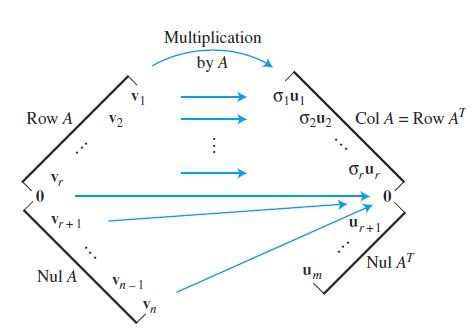
\includegraphics[width=10cm]{week7/fundamental}
\caption{The fundamental spaces and the action of $\bm A$.}
\end{figure}
\subsubsection{Remark 3: vector form}
Recall we can write eigendecomposition in \textit{vector form:}
\[
\bm A=\lambda_1\bm v_1\bm v_1\trans+\dots+\lambda_n\bm v_n\bm v_n\trans
\]
Also, we could write the \emph{general} SVD decomposition in remark 2 into \textit{vector form}:
\[
\bm A=\sigma\bm u_1\bm v_1\trans+\dots+\sigma\bm u_r\bm v_r\trans
\]
where $r=\rank(\bm A)=\text{number of nonzero singular values.}$ Here leads to the third meaning for the rank:
\begin{proposition}
The rank of $m\x n$ matrix $\bm A$ is the number of nonzero singular values.
\end{proposition}
\begin{proof}
Without loss of generality, we set $m\ge n$. And we assume there are exactly $s$ zero singular values of $\bm A$, which means there are $s$ zero eigenvalues of $\bm A\trans\bm A$ assocaiated with their $s$ ind. eigenvectors. (Independence is due to the diagonalizable of $\bm A\trans\bm A$.) In other words, the eigenspace of $\bm A\trans\bm A$ for $\lambda=0$ has dimension $s$.\\
The eigenspace of $\bm A\trans\bm A$ for $\lambda=0$ is given by
\[
\{\bm x:\bm A\trans\bm A\bm x=\bm 0\}.
\]
Hence its dimension is given by
\[
\rank(\bm A\trans\bm A)=\rank(\bm A):=n-r.
\]
Hence $s=n-r$. And obviously, the number of \emph{nonzero} singular values is $n-s=r$.
\end{proof}
\begin{remark}
However, $\rank(\bm A)\ne$ number of nonzero eigenvalues. Let me raise a counterexample:
\[
\bm A=\begin{bmatrix}
0&1\\0&0
\end{bmatrix}
\]
then eigenvalues are $\lambda_1=\lambda_2=0$, and $\rank(\bm A)=1.$
\end{remark}
\subsubsection{Compact SVD}
Hence any matrix with rank $r$ can be factorized into
\begin{align*}
\bm A&=\bm U\bm\Sigma\bm V\trans\\
&=\begin{bmatrix}
\bm u_1&\dots&\bm u_r
\end{bmatrix}\begin{pmatrix}
\sigma_1&&\\&\ddots&\\&&\sigma_r
\end{pmatrix}\begin{bmatrix}
\bm v_1\trans\\\vdots\\\bm v_r\trans
\end{bmatrix}
\end{align*}
where $\bm U\in\mathbb{R}^{m\x r}$ and $\bm V\in\mathbb{R}^{r\x n}$ are both orthogonal matrix. And $\bm\Sigma=\diag(\sigma_1,\dots,\sigma_r)$, where $\sigma_i>0$ for $i=1,2,\dots,r$.
\begin{corollary}
Every rank $r$ matrix can be written as the sum of $r$ rank $1$ matrices. Moreover, these matrices could be perpendicular!
\end{corollary}
What's the meaning of perpendicular?
\begin{definition}[perpendicular for matrix]
For two real $n\x n$ matrix $\bm A$ and $\bm B$, they are said to be \emph{perpendicular} (\emph{orthogonal}) if the inner product between $\bm A$ and $\bm B$ is zero:
\[
\inp{\bm A}{\bm B}=\trace(\bm B\trans\bm A)=\sum_{i,j=1}^{n}\bm A_{ij}B_{ij}=0.
\]
\end{definition}
Decompose $\bm A:=\sum_{i=1}^{r}\sigma_i\bm u_i\bm v_i\trans$. If we set $\bm A_i=\bm u_i\bm v_i\trans\sigma_i$, let's show $\bm A_i$'s are perpendicular:
\begin{align*}
\inp{\bm A_i}{\bm A_j}&=\trace(\bm A_j\trans\bm A_i)\\
&=\trace(\sigma_i\sigma_j\bm v_j\bm u_j\trans\bm u_i\bm v_i\trans)=\sigma_i\sigma_j\trace(\bm v_j\bm u_j\trans\bm u_i\bm v_i\trans)\\
&=\sigma_i\sigma_j\trace(\bm v_j(\bm u_j\trans\bm u_i)\bm v_i\trans)=\sigma_i\sigma_j\trace(\bm v_j\bm 0\bm v_i\trans)\\
&=0.
\end{align*}
So what is rank? How many rank 1 matrices do we need to pick to construct matrix $\bm A$? In fact, this number has no upper bound. For example, if we obtain
\[
\bm A=\bm u_1\bm v_1\trans+\bm u_2\bm v_2\trans
\]
Then we can always decompose any rank 1 matrix into 2 rank 1 matrix:
\[
\bm A=\bm u_1\bm v_1\trans+\frac{1}{2}\bm u_2\bm v_2\trans+\frac{1}{2}\bm u_2\bm v_2\trans.
\]
But this number has a lower bound, that is rank. In other words, $\rank(\bm A)$=smallest number of rank 1 matrices with sum $\bm A$.
\begin{remark}
Up till now, $\rank(\bm A)$ has three meanings:
\begin{itemize}
\item
$\rank(\bm A)=\dim(\row(\bm A))$
\item
$\rank(\bm A)=\dim(\col(\bm A))$
\item
$\rank(\bm A)=$ smallest number of rank 1 matrices with sum $\bm A$.
\end{itemize}
\end{remark}
\subsection{Best Low-Rank Approximation}
Given matrix $\bm A$. What is the \textit{best rank $k$ approximation}? In other words, given matrix $\bm A\in\mathbb{R}^{m\x n}$, what is the optimal solution for the model:
\begin{align*}
  \min\quad        & \|\bm A-\bm Z\|^2_{F} \\
  \text{s.t.\quad} &  \rank(\bm Z)=k &     \\
                   &\bm Z\in\mathbb{R}^{m\x n}
\end{align*}
Firstly let's introduce the definition for Frobenius norm:
\begin{definition}[Frobenius norm]
The Frobenius norm for $m\x n$ matrix $\bm A$ is given by
\[
\|\bm A\|_{F}=\sqrt{\inp{\bm A}{\bm A}}=\sqrt{\trace(\bm A\trans\bm A)}.
\]
\end{definition}
\begin{theorem}\label{proposition_8.4}
Suppose the SVD if $\bm A\in\mathbb{R}^{m\x n}$ is given by
\[
\bm A=\sigma_1\bm u_1\bm v_1\trans+\dots+\sigma_r\bm u_r\bm v_r\trans.
\]
where $\bm u_i$'s and $\bm v_i$'s are $\mathbb{R}^{n}$ vectors. And we suppose $\sigma_1\ge\sigma_2\ge\dots\ge0$.\\
Then the best rank $k$($k\le r$) approximation of $\bm A$ is
\[
\bm A_k=\sigma_1\bm u_1\bm v_1\trans+\dots+\sigma_k\bm u_k\bm v_k\trans.
\]
\end{theorem}
For example, $\sigma_1\bm u_1\bm v_1\trans$ is the best rank 1 approximation.
\subsubsection{Analogy with least square problem}
For least square problem, the key is to do approximation for $\bm b\in\mathbb{R}^m$. In other words, we just do a projection from $\bm b$ to the plane $\{\bm{Ax}|\bm x\in\mathbb{R}^n\}$:
\begin{figure}[H]
\centering\includegraphics{week7/least_square}
\caption{Least square problem: find $\bm x$ such that $\bm{Ax}=\Proj_{\bm A}(\bm b).$}
\end{figure}
Similarly, the beast rank k approximation could be viewed as a projction from $\bm A$ with rank $r$ to the ``plane'' that contains all rank $k$ matrices:
\begin{figure}[H]
\centering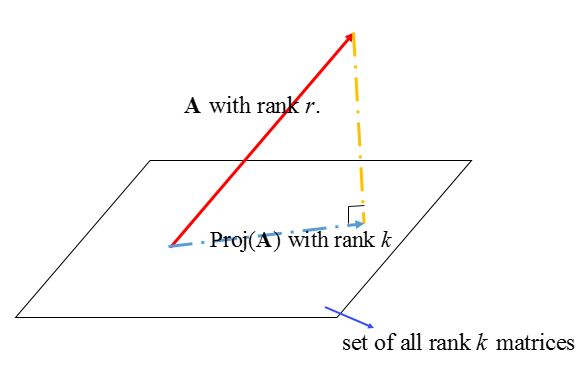
\includegraphics{week7/rank_r}
\caption{Best rank $k$ approximation: find projection from rank $r$ matrix to the plane that contains all rank $k$ matrices}
\end{figure}
\section{Assignment Eight}\index{Assignment_Eight}
\begin{enumerate}
\item
Let $\bm A$ be an $n\x n$ matrix. Show that $\bm A\trans\bm A$ and $\bm A\bm A\trans$ are \textit{similar}.
\item
Let $\bm A$ be $m\times n$ ($m\ge n$) matrix with singular value decomposition $\bm U\Sigma\bm V\trans$. Let $\Sigma^+$ denote the $n\times m$ matrix
\[
\begin{pmatrix}
\frac{1}{\sigma_1}&&&0&\dots&0\\
&\ddots&&\vdots&\ddots&\vdots\\
&&\frac{1}{\sigma_n}&0&\dots&0\\
\end{pmatrix}
\]
And we define $\bm A^+=\bm V\Sigma^+\bm U\trans$
\begin{enumerate}
\item
Show that
\[
\bm A\bm A^+=\begin{bmatrix}
\bm I_n&\bm0\\\bm0&\bm0
\end{bmatrix}\qquad\text{and}\qquad
\bm A^+\bm A=\bm I_n.
\]
(Note that $\bm A^+$ is called the \emph{pseudo-inverse} of $\bm A$.)
\item
If $\rank(\bm A)=n$, Show that $\hat{\bm x}=\bm A^+\bm b$ satisfies the normal equation $\bm A\trans\bm A\bm x=\bm A\trans\bm b.$
\end{enumerate}
\item
Suppose $\bm A\in\mathbb{R}^{m\x n}(m\ge n)$ has an SVD 
\[
\bm A=\sigma_1\bm u_1\bm v_1\trans+\dots+\sigma_n\bm u_n\bm v_n\trans
\]
where $\sigma_1\ge\sigma_2\ge\dots\ge\sigma_n\ge0.$
\begin{enumerate}
\item
Prove that $\|\bm A\|_{F}^2=\sum_{i=1}^{n}\sigma_i^2$.
\item
Let $\bm A_k$ be the \textit{best rank-k approximation} of $\bm A$, what is $\|\bm A-\bm A_k\|_{F}$?
\end{enumerate}
\item
Suppose the \textit{maximal singular value} of $\bm A\in\mathbb{R}^{m\x n}$ is $\sigma_1$, prove 
\[
\sigma_1=\max_{\bm x,\bm y}\bm x\trans\bm A\bm y
\]
where $\bm x\in\mathbb{R}^m,\bm y\in\mathbb{R}^n,\|\bm x\|=\|\bm y\|=1.$
\item
Let $\bm A$ be a \textit{symmetric positive definite} $n\x n$ matrix. Show that $\bm A$ can be factored into a product $\bm Q\bm Q\trans$, where $\bm Q$ is an $n\x n$ matrix whose columns are \textit{mutually orthogonal.}
\end{enumerate}
%\include{week8/Lecture_1}
%\include{week8/Lecture_2}
%\include{week9/Lecture_1}
%\include{week9/Lecture_2}
%\include{week10/Lecture_1}
%\include{week10/Lecture_2}
%\include{week11/Lecture_1}
%\include{week11/Lecture_2}
%\include{week12/Lecture_1}
%\include{week12/Lecture_2}
%\include{week13/Lecture_1}
%\include{week13/Lecture_2}
%\include{week14/Lecture_1}
%\include{week14/Lecture_2}


\chapter{Final Exam}

\section{Sample Exam}\index{Sample Exam}
DURATION OF EXAMINATION: 2 hours in-class\\
\textit{This examination paper includes $6$ pages and $6$ problems. You are responsible for ensuring that
your copy of the paper is complete. Bring any discrepancy to the attention of your invigilator.}\\
\begin{enumerate}
\item \textbf{(20 points)} \textit{Matrix representation for linear transformation}\\
Let $D$ be defined as (\textit{differentiate operator}):
\[
D(f)=\frac{\diff f}{\diff x}
\]
Consider the space $\Span\{\sin x,\cos x,\sin 2x,\cos 2x\}.$
\begin{enumerate}
\item
Write down a \textit{matrix representation} of $T$ with respect to the basis $\{\sin x,\cos x,\sin 2x,\cos 2x\}.$\\
\item
If a polynomial $f(x)$ satisfies
\[
T(f)=\lambda f,
\]
we say $f$ is an \textit{eigenvector} of $T$.\\
Find $4$ \textit{linearly independent} eigenvectors of $D^2$. In other words, find $f_k$ such that
\[
D^2(f_k)=\lambda_kf_k
\]
for $k=1,2,3,4$.
\end{enumerate}
\newpage
\item \textbf{(20 points)} \textit{Least Square Method}\\
\begin{enumerate}
\item
Find the \textit{least squares fit line} $y=C+Dx$ to the following 3 data points:
\begin{figure}[H]
\centering
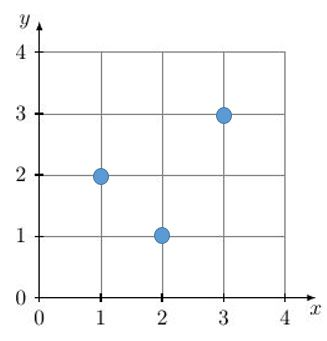
\includegraphics[width=7cm]{exam/final/least_square}
\end{figure}
\item
Let $\bm A$ be a matrix with \textit{linearly independent columns} and consider the \textit{projection matrix} $\bm P=\bm A(\bm A\trans\bm A)^{-1}\bm A\trans$. What are the possible eigenvalues for $\bm P$? Give your reasons.
\end{enumerate}
\newpage
\item \textbf{(20 points)} \\
True or False. No justifications are required.
\begin{enumerate}
\item
For real symmetric matrix $\bm A$, if $\bm A\succ 0$, then $\bm A^{-1}$ exists and $\bm A^{-1}\succ0.$\\
\item
If $\bm A$ is a matrix, (Note that $\bm A$ may not be real) then any element of the \textit{kernel} of $\bm A$ is \textit{perpendicular} to any element of the \textit{image} of $\bm A\trans$.\\
\item
The only $m\x n$ matrix of rank $0$ is $\bm 0$.\\
\item
Let $\bm A$ be real square matrix. If $\bm x$ is in $N(\bm A)$ and $\bm y$ is in $C(\bm A\trans)$, then $\bm x\bm y\trans=0.$\\
\item
If $\bm A$ and $\bm B$ are \textit{diagonalizable} matrices, then $\begin{bmatrix}
\bm A&\bm 0\\\bm 0&\bm B
\end{bmatrix}$ is \textit{diagonalizable}.
\end{enumerate}
\newpage
\item \textbf{(20 points)} \textit{SVD decomposition} \\
\begin{enumerate}
\item
Find the limiting values of $y_k$ and $z_k$ $(k\rightarrow\infty)$:
\[
\left\{
\begin{aligned}
y_{k+1}&=0.8y_k+0.3z_k,\\
z_{k+1}&=0.2y_k+0.7z_k,
\end{aligned}
\right.
\]
And $y_0=0,z_0=5.$\\
\textit{Hint: Show that $\begin{bmatrix}
0.8&0.3\\0.2&0.7
\end{bmatrix}$ is similar to $\begin{bmatrix}
0.5&0\\0&1
\end{bmatrix}.$}
\item
Find the SVD of the matrix $\begin{pmatrix}
0.5&0\\0&1
\end{pmatrix}.$
\end{enumerate}
\newpage
\item \textbf{(15+5 points)} \textit{Eigenvalues and Eigenvectors}\\
Given a \textit{real symmetric} matrix $\bm A$, the \emph{Rayleigh quotient} $R(\bm x)$ is defined as
\[
R(\bm x)=\frac{\bm x\trans\bm A\bm x}{\bm x\trans\bm x}\text{ for }\bm x\ne\bm0.
\]
Suppose the \textit{eigenvalues} of $\bm A$ are
$\lambda_1\le\lambda_2\le\dots\le\lambda_n$.
\begin{enumerate}
\item
Prove that the minimum eigenvalue $\lambda_1$ is the minimal value of $R(\bm x)$. 
\[
\text{i.e. }\lambda_1=\min_{\bm x\in\mathbb{R}^n-\{\bm 0\}}R(\bm x).
\]
\item
Suppose $\bm x_1$ is the eigenvector associated with $\lambda_1$, i.e. $\bm A\bm x_1=\lambda_1\bm x_1$.
\[
\text{Prove that }\lambda_2=\min_{\bm y\trans\bm x_1=0}R(\bm y).
\]
\item \textbf{(bonus question)}\\
Suppose $\bm v\in\mathbb{R}^n$ is an arbitrary given vector.
\[
\text{Prove that }\lambda_2\ge\min_{\bm y\trans\bm v=0}R(\bm y).
\]
\end{enumerate}
\newpage
\item \textbf{(10 points)} \textit{Positive semi-definite}\\
\begin{definition}[diagonal dominant]\qquad\\
A matrix $\bm M\in\mathbb{R}^{n\x n}$ is called \emph{diagonal dominant} if for $\forall i\in\{1,2,\dots,n\}$,
\[
|\bm M_{ii}|\ge\sum_{j\ne i}|\bm M_{ij}|.
\]
It is called \emph{strictly diagonal dominant} if for $\forall i\in\{1,2,\dots,n\}$,
\[
|\bm M_{ii}|>\sum_{j\ne i}|\bm M_{ij}|.
\]
\end{definition}
Prove the following statements:
\begin{enumerate}
\item
$\bm Z=\begin{pmatrix}
5&1&4\\1&5&3\\4&3&7
\end{pmatrix}$ is \textit{positive semi-definite}.
\item
If $\bm M$ is \textit{symmetric} and \textit{diagonal dominant}, then $\bm M\succeq0.$
\end{enumerate}
\end{enumerate}






\section{Final Exam}\index{Sample Exam}
DURATION OF EXAMINATION: 2 hours and 35 minutes in-class\\
\textit{This examination paper includes $6$ pages and $6$ problems. You are responsible for ensuring that
your copy of the paper is complete. Bring any discrepancy to the attention of your invigilator.}\\
\begin{enumerate}
\item \textbf{(20 points)} \textit{Matrix representation for linear transformation}\\
\begin{enumerate}
\item
Let $T$ be the transformation
\begin{gather*}
T:\{\textbf{polynomials of degree $\le4$}\}\mapsto\{\textbf{polynomials of degree $\le4$}\}\\
\qquad\qquad\qquad\qquad\qquad T(p)=(x-2)\frac{\diff p}{\diff x}
\end{gather*}
Show that $T$ is a \textit{linear transformation} and write down a \textit{matrix representation} of $T$ with respect to basis $\{1,x,x^2,x^3,x^4\}$ for the input and output space.\\
\item
If a polynomial $f(x)$ satisfies
\[
T(f)=\lambda f,
\]
we say $f$ is an \textit{eigenvector} of $T$. Find two \textit{linearly independent} eigenvectors of $T$.
\end{enumerate}
\newpage
\item \textbf{(20 points)} \textit{Least Square Method}\\
\begin{enumerate}
\item
Find the projection of $\bm z=\begin{bmatrix}
1\\0\\1
\end{bmatrix}$ onto the column space of $\begin{bmatrix}
1&-1\\1&-1\\-2&4
\end{bmatrix}.$\\
\item
Let $\mathcal{A}:\mathbb{R}^{2\x 1}\mapsto\mathbb{R}^{2\x 2}$ be a mapping defined as
\[
\mathcal{A}\begin{bmatrix}
a\\b
\end{bmatrix}=\begin{bmatrix}
a+b&a-b\\-2a+4b&0
\end{bmatrix},\forall a,b\in\mathbb{R}.
\]
Define $\kappa=\{\bm{Ax}|\bm x\in\mathbb{R}^{2\x 1}\}$.\\
Find the best approximation of $\bm B=\begin{bmatrix}
1&2\\7&1
\end{bmatrix}$ in the space $\kappa$.\\
%\textit{Hint: Consider $\begin{bmatrix}
%1&2\\7&1
%\end{bmatrix}$ and $\begin{bmatrix}
%a+b&a-b\\-2a+4b&0
%\end{bmatrix}$ as $\mathbb{R}^{4\x 1}$ vector.\\
%Then you only need to find the best approximation of $\begin{pmatrix}
%1\\2\\7\\1
%\end{pmatrix}$ onto the set $\{\bm{Ax}|\bm x\in\mathbb{R}^{2\x 1}\}$, where $\bm A=\begin{bmatrix}
%1&1\\1&-1\\-2&4\\0&0
%\end{bmatrix}.$}
\end{enumerate}
\newpage
\item \textbf{(20 points)} \\
True or False. No justifications are required.
\begin{enumerate}
\item
If all the entries of a square matrix $\bm A$ are \textit{positive}, then $\bm A^{-1}$ exist.\\
\item
If $\bm Q$ is an \textit{orthogonal matrix}, then $\det(\bm Q)=\pm1$.\\
\item
If $\bm A$ is a \textit{negative definite} matrix, then its singular values have the same absolute values as its eigenvalues.\\
\textit{Hint: Note that $\bm A$ is said to be negative definite when $-\bm A$ is positive definite.}\\
\item
If $\bm A$ is an $n\x n$ matrix with \textit{characteristic polynomial} $p_{\bm A}(t)=t^n$, then $\bm A=\bm 0.$\\
\item
If $\bm A$ is the sum of 5 rank one matrices, then $\rank(\bm A)\le5.$
\end{enumerate}
\newpage
\item \textbf{(20 points)} \textit{SVD decomposition} \\
The question is about the matrix
\[
\bm A=\begin{bmatrix}
0&-1\\4&0
\end{bmatrix}
\]
\begin{enumerate}
\item
Find its eigenvalues and eigenvectors, write the vector $\bm u=\begin{bmatrix}
2\\0
\end{bmatrix}$ as a combination of those eigenvectors.\\
\item
Do the SVD decomposition to derive $\bm A=\bm U\Sigma\bm V\trans$ in two steps:
\begin{itemize}
\item
First, compute $\bm V$ and $\Sigma$ using the matrix $\bm A\trans\bm A$.
\item
Second, find the (\textit{orthonormal}) columns of $\bm U$.
\end{itemize}
\end{enumerate}
\newpage
\item \textbf{(15+5 points)} \textit{Eigenvalues and Eigenvectors}\\
\begin{enumerate}
\item
Suppose $\bm A,\bm B\in\mathbb{R}^{n\x n}$ can can be \textit{diagonalized} by the same matrix, prove that $\bm{AB}=\bm{BA}.$\\
%\textit{Hint: Note that $\bm A$ is said to be diagonalized by $\bm S$ if $\bm S^{-1}\bm A\bm S$ is diagonal.}\\
\item
Suppose $\bm A,\bm B\in\mathbb{R}^{n\x n}$ satisfy $\bm{AB}=\bm{BA}$, and both $\bm A$ and $\bm B$ are diagonalizable. $\bm A$ has $n$ \textit{distinct} eigenvalues. Prove that $\bm A,\bm B$ can can be \textit{diagonalized} by the same matrix.\\
%\textit{Hint: Suppose $\bm A$ has eigenvectors $\bm v_1,\dots,\bm v_n$. You can express $\bm B\bm v_i$ as linear combination of $\bm v_1,\dots,\bm v_n$. Then you can express $\bm A(\bm B\bm v_i)$ and $\bm B(\bm A\bm v_i)$. Finally compute $\bm A(\bm B\bm v_i)-\bm B(\bm A\bm v_i)$ to derive something.}\\
\item \textbf{(bonus question)}\\
Prove part $(b)$ without the assumption that $\bm A$ has $n$ \textit{distinct} eigenvalues. (i.e. $\bm A$ might have \emph{repeated} eigenvalues)\\
%\textit{Hint: Since $\bm A$ is diagonalizable, there exists $\bm Q$ such that $\bm Q^{-1}\bm A\bm Q=\bm D$, where $\bm D$ is diagonal. Then you should express $\bm D$. Then you compute $\bm Q^{-1}\bm B\bm Q=\bm C$, i.e. partition $\bm C$ in the same way of $\bm D$. Next you should show us that $\bm C$ is block diagonal. Then you construct \emph{diagonal} matrix $\bm T_*$ that diagonalize $\bm C$. Finally you construct $\bm P$ that diagonalize both $\bm A$ and $\bm B$.}
\end{enumerate}
\newpage
\item \textbf{(10 points)} \textit{Positive definite}\\
Suppose $\bm A,\bm B\in\mathbb{R}^{n\x n}$, where $\bm A=\begin{bmatrix}
a_{ij}
\end{bmatrix}_{i,j=1}^{n}, \bm B=\begin{bmatrix}
b_{ij}
\end{bmatrix}_{i,j=1}^{n}$.\\
Define the \emph{Hadamard product} $\bm A\circ\bm B$ as an $n\x n$ matrix with entries
\[
\begin{bmatrix}
\bm A\circ\bm B
\end{bmatrix}_{ij}=a_{ij}b_{ij}.
\]
For example, if $\bm A=\begin{bmatrix}
1&2\\3&7
\end{bmatrix},\bm B=\begin{bmatrix}
0&\pi\\1&e
\end{bmatrix},$ then $\bm A\circ\bm B=\begin{bmatrix}
0&2\pi\\3&7e
\end{bmatrix}.$\\
Prove the following statements:
\begin{enumerate}
\item
$\rank(\bm A\circ\bm B)\le\rank(\bm A)\rank(\bm B)$;
\\
%\textit{Hint: Extend Hadamard product into vector. Then it's easy to verify that $(\bm A\circ\bm B)\circ\bm C=\bm A\circ\bm C+\bm B\circ\bm C$ and $(\bm u_1\bm v_1\trans)\circ(\bm u_2\circ\bm v_2\trans)=(\bm u_1\circ\bm u_2)\x(\bm v_1\circ\bm v_2)\trans$. Then you can do SVD decomposition for $\bm A$ and $\bm B$ (vector form, related to rank.) Then you can express $\bm A\circ\bm B$ as the sum of some matrices with rank 1.}
\\
\item
If $\bm A\succeq0,\bm B\succeq0$ and $\bm A,\bm B$ are \textit{symmetric matrix}, prove that
\[
\bm A\circ\bm B\succeq0.
\]
%\textit{Hint: Note that $\bm A=\bm R\trans\bm R$, where $\bm R$ is square. Then you should express $\bm R\trans\bm R$ into vector form. Similarly, you can express $\bm B$ into vector form. Then you compute $\bm A\circ\bm B$ and show it is PSD by definition.}
\end{enumerate}
\end{enumerate}


\chapter{Solution}

\section{Assignment Solutions}\index{Assignment Solution}
\subsection{Solution to Assignment One}
\begin{enumerate}
\item 
\begin{proof}[Solution.]
Firstly we do the elimination shown as below:
\[\begin{bmatrix}
a & 2 & 3 \\ a & a & 4 \\ a & a & a
\end{bmatrix}\implies\begin{bmatrix}
a & 2 & 3 \\ 0 & a-2 & 1 \\ 0 & a-2 & a-3
\end{bmatrix}\implies
\begin{bmatrix}
a & 2 & 3 \\ 0 & a-2 & 1 \\ 0 & 0 & a-4
\end{bmatrix}\]
Here in order to give three pivots we need to let the diagonal be nonzero, which is to say:
\[
a = 0 \qquad\text{or}\qquad a-2=0 \qquad\text{or}\qquad a-4 = 0
\] 
\[\implies a = 0 \qquad\text{or}\qquad a=2 \qquad\text{or}\qquad a=4\]
\end{proof}




\item
let's solve this problem by answering the following questions first.
\begin{enumerate}
\item
The other solution is given by:$(m_1x+m_2X,m_1y+m_2Y,m_1z+m_2Z)$, where $m_1+m_2=1$.
\item
They also meet the line that passes these two points
\item
In $\mathbb{R}^{n}$ space we can also ensure every point on the line that determined by the two solutions is also a solution.
\end{enumerate}
Then let's proof the begining statement rigorously:
\begin{proof}
Assume the system of equation is given by 
\begin{gather}
a_{11}x_1 + a_{12}x_2 + \dots + a_{1n}x_n = b_1 \notag \\ 
a_{21}x_1 + a_{22}x_2 + \dots + a_{2n}x_n = b_2 \notag \\
\dots 	\notag 	\\
a_{m1}x_1 + a_{m2}x_2 + \dots + a_{mn}x_n = b_m  \label{eq:linear system equations}
\end{gather}
where it contains two solutions $(y_1,y_2,\dots,y_n)$ and $(z_1,z_2,\dots,z_n)$. Let's show that every point on the line that determined by the two solutions is also a solution. In other words, once the system has two solutions, it will contain infinitely many solutions.

\qquad Any point on the line that determined by the two solutions is given by 
\[(m_1y_1+m_2z_1,\dots,m_1y_n+m_2z_n),\qquad \text{where } m_1+m_2=1\]
And then we show that this point is also a solution to this system:\\
\hspace*{1cm} for the $i$th linear equation it satisfies that 
\[
\left\{ \begin{aligned}
a_{i1}y_1 + a_{i2}y_2 + \dots + a_{in}y_n = b_i \\
a_{i1}z_1 + a_{i2}z_2 + \dots + a_{in}z_n = b_i
\end{aligned}
\right.
\]
\qquad Hence we set $x_j = m_1y_j+m_2z_j$ for $j = 1,2,\dots,n$. Then we obtain:
\begin{align*}
a_{i1}x_1 + a_{i2}x_2 + \dots + a_{in}x_n&\\ &= a_{i1}(m_1y_1+m_2z_1) + a_{i2}(m_1y_2+m_2z_2) + \dots + a_{in}(m_1y_n+m_2z_n)\\ &= m_1(a_{i1}y_1 + a_{i2}y_2 + \dots + a_{in}y_n) + m_2(a_{i1}z_1 + a_{i2}z_2 + \dots + a_{in}z_n)\\ &= m_1b_i + m_2b_i = (m_1+m_2)b_i=b_i.
\end{align*}
\qquad where $ i= 1,2,\dots,m$

Since the choice of point on the line was arbitrary, we see that every point on the line determined by the two solutions is also a solution, so there are infinitely many solutions to the system
\end{proof}

\item \begin{proof}[Solution.]
\begin{enumerate}
\item
We begin to do the elimination for the system:
\[
\left[
\begin{array}{@{}rrr|r@{}}
1 & 4 & -2 & 1 \\
1 & 7 & -6 & 6 \\
0 & 3 & q & t\\
\end{array}
\right]
\xLongrightarrow{\text{Add $(-1)\times$ row 1 to row 2}}
\left[
\begin{array}{@{}ccc|c@{}}
1 & 4 & -2 & 1 \\
0 & 3 & -4 & 5 \\
0 & 3 & q & t
\end{array}
\right]\]
\[
\xLongrightarrow{\text{Add $(-1)\times$ row 2 to row 3}}
\left[
\begin{array}{@{}ccc|c@{}}
1 & 4 & -2 & 1 \\
0 & 3 & -4 & 5 \\
0 & 0 & \cellcolor{black!20}{q+4} & t-5
\end{array}
\right]
\]
In order to make this system singular we need to make the third row has no pivot.$\implies q+4=0\implies q = -4$. In order to give infinitely many solutions we have to let the third equation satisfies $0=0$. $\implies t-5=0 \implies t=5$.
\item
When $z=1$, the second equation $3y-4z=5$ gives $y=3$; \\ the third equation $x+4y-2z=1$ gives $x=-9$.

\end{enumerate}
\end{proof}

\item 
\begin{proof}[Solution.]
\begin{enumerate}
\item \[\bm A = \begin{bmatrix}0 & 1 \\ -1 & 0\end{bmatrix}
\implies \bm A^2 = \begin{bmatrix}0 & 1 \\ -1 & 0\end{bmatrix}\begin{bmatrix}0 & 1 \\ -1 & 0\end{bmatrix} 
= \begin{bmatrix}-1 & 0 \\ 0 & -1\end{bmatrix}\]
\item
\[\bm B = \begin{bmatrix}0 & 1 \\ 0 & 0\end{bmatrix}
\implies \bm B^2 = \begin{bmatrix}0 & 1 \\ 0 & 0\end{bmatrix}\begin{bmatrix}0 & 1 \\ 0 & 0\end{bmatrix} 
= \begin{bmatrix}0 & 0 \\ 0 & 0\end{bmatrix} = \bm 0 \]
\item
\[
\bm C = \begin{bmatrix}0 & 1 \\ 1 & 0\end{bmatrix};\bm D = \begin{bmatrix}0 & 1 \\ -1 & 0\end{bmatrix}
\implies \bm{CD} = \begin{bmatrix}0 & 1 \\ 1 & 0\end{bmatrix}\begin{bmatrix}0 & 1 \\ -1 & 0\end{bmatrix} = 
\begin{bmatrix}-1 & 0 \\ 0 & 1\end{bmatrix} = -\bm{DC}
\]
\item
\[\bm E = \begin{bmatrix}1 & 1 \\ -1 & -1\end{bmatrix};\bm F = \begin{bmatrix}-1 & -1 \\ 1 & 1\end{bmatrix}
\implies \bm{EF} = \begin{bmatrix}0 & 0 \\ 0 & 0\end{bmatrix}= \bm{0}
\]
\end{enumerate}\end{proof}

\item
\begin{proof}
We assume $\bm A$ is a $m\times n$ matrix,$\bm B$ is a $n\times p$ matrix,$\bm C$ is a $p\times q$ matrix which is given by:
\[ \bm A := \begin{bmatrix}a_{ij}\end{bmatrix},\bm B := \begin{bmatrix}b_{ij}\end{bmatrix},
\bm C := \begin{bmatrix}c_{ij}\end{bmatrix}.
\]
And we also define:
\[
\bm{AB} := \bm{D} := \begin{bmatrix}d_{ij}\end{bmatrix},
\bm{BC} := \bm{E} := \begin{bmatrix}e_{ij}\end{bmatrix}.
\]
Obviously, $\bm{AB}$ and $\bm{BC}$ are well-defined and they are all $m \times q$ matrix.\\
\textbullet According to the definition for multiplication, $d_{ij} = \sum_{k=1}^n a_{ik}b_{kj}$. We define $(\bm{AB})\bm{C} := \bm{H} = \begin{bmatrix}h_{ij}\end{bmatrix}$, thus
\[
h_{ij} = \sum_{l=1}^p d_{il}c_{lj} = \sum_{l=1}^p(\sum_{k=1}^n a_{ik}b_{kl})c_{lj} = \sum_{k=1}^n\sum_{l=1}^pa_{ik}b_{kl}c_{lj}
\]
where $i=1,2,\dots,m$ and $i=1,2,\dots,q$.\\
\textbullet On the other hand, $e_{ij} = \sum_{l=1}^p b_{il}c_{lj}$. We define $\bm{A}(\bm{BC}) := \bm{G} = \begin{bmatrix}g_{ij}\end{bmatrix}$, thus
\[
g_{ij} = \sum_{k=1}^n a_{ik}e_{kj} = \sum_{k=1}^n(\sum_{l=1}^p b_{kl}c_{lj})a_{ik} = \sum_{k=1}^n\sum_{l=1}^pa_{ik}b_{kl}c_{lj}
\]
where $i=1,2,\dots,m$ and $i=1,2,\dots,q$.\\
Hence we have $h_{ij} = g_{ij}$, $i=1,2,\dots,m$ and $i=1,2,\dots,q$. 
Hence we have $\bm H = \bm G \implies (\bm{AB})\bm{C}=\bm{A}(\bm{BC})$.
\end{proof}

\item
\begin{proof}[Solution.] \qquad \\
For matrix $\bm A = \begin{bmatrix}
4 & 0 & 4 \\ 6 & 6 & -8 \\ -9 & 5 & -8
\end{bmatrix}$, we can split $\bm A$ into blocks $\bm A = 
\left[
\begin{array}{cc|c}
4 & 0 & 4 \\ 
6 & 6 & -8 \\
\hline
-9 & 5 & -8
\end{array}
\right]
 = \begin{bmatrix}
A_1 & A_2 \\ A_3 & A_4
\end{bmatrix}$,
where $A_1 = \begin{bmatrix}4 & 0 \\ 6 & 6\end{bmatrix}, A_2 = \begin{bmatrix}
4 \\ -8
\end{bmatrix}, A_3 = \begin{bmatrix}
-9 & 5
\end{bmatrix}, A_4 = \begin{bmatrix}
-8
\end{bmatrix}.$\\
For matrix $\bm B = \begin{bmatrix}
8 & -3 & -7 \\ 3 & -7 & -4 \\ 4 & -4 & 1
\end{bmatrix}$, we can split $\bm B$ into blocks $\bm B = 
\left[
\begin{array}{cc|c}
8 & -3 & -7 \\ 3 & -7 & -4 \\
\hline
4 & -4 & 1
\end{array}
\right]
 = \begin{bmatrix}
B_1 & B_2 \\ B_3 & B_4
\end{bmatrix}$,
where $B_1 = \begin{bmatrix}8 & -3 \\ 3 & -7\end{bmatrix}, B_2 = \begin{bmatrix}
-7\\ -4
\end{bmatrix}, B_3 = \begin{bmatrix}
4 & -4
\end{bmatrix}, B_4 = \begin{bmatrix}
1
\end{bmatrix}.$\\
We let $\bm C = \bm A \bm B = \begin{bmatrix}
C_1 & C_2 \\ C_3 & C_4
\end{bmatrix}, $we can find $C_1,C_2,C_3,C_4$ in two different ways, if we get the same answers, we can verify the block multiplication succeeds.
\begin{enumerate}
\item
Multiply $\bm A$ times $\bm B$ to find $\bm C = 
\left[
\begin{array}{cc|c}
48 & -28 & -24 \\ 34 & -28 & -74 \\
\hline
-89 & 24 & 35
\end{array}
\right],$\\
Hence $C_1 = \begin{bmatrix}
48 & -28 \\ 34 & -28
\end{bmatrix}, C_2 = \begin{bmatrix}
-24 \\ -74
\end{bmatrix},C_3 = \begin{bmatrix}
-89 & 24
\end{bmatrix}, C_4 = \begin{bmatrix}
35
\end{bmatrix}.$
\item
On the other hand, we have $\begin{bmatrix}
A_1 & A_2 \\ A_3 & A_4
\end{bmatrix}\begin{bmatrix}
B_1 & B_2 \\ B_3 & B_4
\end{bmatrix} = \begin{bmatrix}
A_1B_1+A_2B_3 & A_1B_2+A_2B_4 \\ A_3B_1+A_4B_3 & A_3B_2+A_4B_4
\end{bmatrix}$\\
Hence we find $C_1 =A_1B_1+A_2B_3 = \begin{bmatrix}4 & 0 \\ 6 & 6\end{bmatrix}\begin{bmatrix}8 & -3 \\ 3 & -7\end{bmatrix}+\begin{bmatrix}
4 \\ -8
\end{bmatrix}\begin{bmatrix}
4 & -4
\end{bmatrix} = 
 \begin{bmatrix}
48 & -28 \\ 34 & -28
\end{bmatrix}.$\\Similarly, we have
\[
C_2 = A_1B_2+A_2B_4 = \begin{bmatrix}
-24 \\ -74
\end{bmatrix}
\]
\[
C_3 = A_3B_1+A_4B_3 = \begin{bmatrix}
-89 & 24
\end{bmatrix}\]
\[
C_4 = A_3B_2+A_4B_4 = \begin{bmatrix}
35
\end{bmatrix}.
\]
\end{enumerate}






\end{proof}







\enlargethispage{1cm}
\item
\begin{proof}[Solution.]
\[
\bm A = \begin{bmatrix}
a & a & a & a \\ a & b & b & b \\ a & b & c & c \\ a & b & c & d
\end{bmatrix}\xLongrightarrow{\bm E_{41}\bm E_{31}\bm E_{21}}\begin{bmatrix}
a & a & a & a \\ 0 & b-a & b-a & b-a \\ 0 & b-a & c-a & c-a \\ 0 & b-a & c-a & d-a
\end{bmatrix}\]\[\xLongrightarrow{\bm E_{42}\bm E_{32}}\begin{bmatrix}
a & a & a & a \\ 0 & b-a & b-a & b-a \\ 0 & 0 & c-b & c-b \\ 0 & 0 & c-b & d-b
\end{bmatrix}\xLongrightarrow{\bm E_{43}}\begin{bmatrix}
a & a & a & a \\ 0 & b-a & b-a & b-a \\ 0 & 0 & c-b & c-b \\ 0 & 0 & 0 & d-c
\end{bmatrix} = \bm U
\]
\[\implies\bm E_{43}\bm E_{42}\bm E_{32}\bm E_{41}\bm E_{31}\bm E_{21}\bm A = \bm U\implies \bm A = \bm E_{21}^{-1}\bm E_{31}^{-1}\bm E_{41}^{-1}\bm E_{32}^{-1}\bm E_{42}^{-1}\bm E_{43}^{-1}\bm U
\]
\[\implies 
\bm A = \begin{bmatrix}
a & a & a & a \\ a & b & b & b \\ a & b & c & c \\ a & b & c & d
\end{bmatrix} = \begin{bmatrix}
1 & 0 & 0 & 0 \\ 1 & 1 & 0 & 0 \\ 1 & 1 & 1 & 0 \\ 1 & 1 & 1 & 1
\end{bmatrix}\left[
\begin{array}{@{}cccc@{}}
\cellcolor{black!20}{a} & a & a & a \\
0 & \cellcolor{black!20}{b-a} & b-a & b-a \\
0 & 0 & \cellcolor{black!20}{c-b} & c-b \\
0 & 0 & 0 & \cellcolor{black!20}{d-c} \\
\end{array}
\right]
\]
\[
\implies \bm{L} = \begin{bmatrix}
1 & 0 & 0 & 0 \\ 1 & 1 & 0 & 0 \\ 1 & 1 & 1 & 0 \\ 1 & 1 & 1 & 1
\end{bmatrix}; \qquad \bm{U} = \left[
\begin{array}{@{}cccc@{}}
\cellcolor{black!20}{a} & a & a & a \\
0 & \cellcolor{black!20}{b-a} & b-a & b-a \\
0 & 0 & \cellcolor{black!20}{c-b} & c-b \\
0 & 0 & 0 & \cellcolor{black!20}{d-c} \\
\end{array}
\right]
\]
In order to get four pivots, we need to let the diagonal entries of $\bm U$ to be nonzero.
\[\implies a\ne 0 \qquad a \ne b \qquad b\ne c\qquad c\ne d   \]
\end{proof}
\end{enumerate}
\subsection{Solution to Assignment Two}
\begin{enumerate}
\item
\begin{proof}[Proof.]
\begin{proof}[Sufficiency.]\qquad \\
If $\bm M$ is invertible, then there exists matrix $\bm N$ such that $\bm M\bm N = \bm N\bm M = \bm I$.
\[\implies
(\bm{ABC})\bm N = \bm I,\bm N(\bm{ABC})=\bm I.
\implies
\bm A(\bm{BCN}) = \bm I,(\bm{NAB})\bm C = \bm I.
\]
$\implies \bm{BCN}$ is the right inverse of $\bm A$, $\bm{NAB}$ is the left inverse of $\bm C$. 
\\Hence $\bm A$ and $\bm C$ is invertible.\\
Moreover, $(\bm{ABC})\bm N = \bm I \implies (\bm{AB})\bm{CN} = \bm I$. Hence $\bm{CN}$ is the right inverse of $\bm{AB}$. 
\\Hence $\bm{AB}$ is invertible. Hence there exists $(\bm{AB})^{-1}$ such that $((\bm{AB})^{-1})(\bm{AB}) = \bm I$.\\$\implies ((\bm{AB})^{-1}\bm A)\bm B = \bm I$. Hence $(\bm{AB})^{-1}\bm A$ is the left inverse of $\bm B$. \\Hence $\bm B$ is invertible.
\begin{proof}[Necessity.]\qquad \\
If $\bm A,\bm B,\bm C$ is invertible, then there exist $\bm A^{-1},\bm B^{-1},\bm C^{-1}$ such that \[\bm A\bm A^{-1} = \bm I,\bm B\bm B^{-1} = \bm I,\bm C\bm C^{-1} = \bm I.\]
\[
\begin{split}
\implies \bm{ABC}(\bm C^{-1}\bm B^{-1}\bm A^{-1}) &=\bm{AB}(\bm C\bm C^{-1})(\bm B^{-1}\bm A^{-1}) = \bm{AB}\bm I(\bm B^{-1}\bm A^{-1}) 
\\&= \bm{AB}(\bm B^{-1}\bm A^{-1}) = \bm A(\bm B\bm B^{-1})\bm A^{-1} = \bm A\bm I\bm A^{-1} \\
&= \bm A\bm A^{-1} = \bm I.
\end{split}
\]
Hence $\bm C^{-1}\bm B^{-1}\bm A^{-1}$ is the right inverse of $\bm{ABC}$. Hence $\bm{ABC}$ is invertible.
\end{proof}
\end{proof}
\end{proof}
\item
\begin{proof}[Solution.]
The inverse are respectively given by $
\begin{bmatrix}
\bm I&\bm 0\\-\bm C&\bm I
\end{bmatrix}, \begin{bmatrix}
\bm A^{-1}&\bm 0\\ -\bm D^{-1}\bm C\bm A^{-1}&\bm D^{-1}
\end{bmatrix}, \begin{bmatrix}
-\bm D&\bm I\\\bm I&\bm 0
\end{bmatrix}.$
\begin{itemize}
\item
\[
\begin{bmatrix}
\bm I&\bm 0\\\bm C&\bm I
\end{bmatrix}
\begin{bmatrix}
\bm I&\bm 0\\-\bm C&\bm I
\end{bmatrix} = \begin{bmatrix}
\bm I\bm I+\bm 0(-\bm C)&\bm I\bm 0+\bm 0\bm I\\
\bm C\bm I+\bm I(-\bm C)&\bm C\bm 0+\bm I\bm I
\end{bmatrix}= \begin{bmatrix}
\bm I&\bm 0\\\bm 0&\bm I
\end{bmatrix}
\]
Hence $\begin{bmatrix}
\bm I&\bm 0\\-\bm C&\bm I
\end{bmatrix}$ is the right inverse of $\begin{bmatrix}
\bm I&\bm 0\\\bm C&\bm I
\end{bmatrix}$, hence $\begin{bmatrix}
\bm I&\bm 0\\-\bm C&\bm I
\end{bmatrix}$ is the inverse of $\begin{bmatrix}
\bm I&\bm 0\\\bm C&\bm I
\end{bmatrix}$.
\newpage

\item
\[
\begin{bmatrix}
\bm A&\bm 0\\\bm C&\bm D
\end{bmatrix}\begin{bmatrix}
\bm A^{-1}&\bm 0\\ -\bm D^{-1}\bm C\bm A^{-1}&\bm D^{-1}
\end{bmatrix}
 = \begin{bmatrix}
\bm A\bm A^{-1}+\bm 0(-\bm D^{-1}\bm C\bm A^{-1})&\bm A\bm 0+\bm 0\bm D^{-1}\\
\bm C\bm A^{-1}+\bm D(-\bm D^{-1}\bm C\bm A^{-1})&\bm C\bm 0+\bm D\bm D^{-1}
\end{bmatrix}
=\begin{bmatrix}
\bm I&\bm 0\\\bm 0&\bm I
\end{bmatrix}
\]
Hence $\begin{bmatrix}
\bm A^{-1}&\bm 0\\ -\bm D^{-1}\bm C\bm A^{-1}&\bm D^{-1}
\end{bmatrix}$ is the right inverse of $\begin{bmatrix}
\bm A&\bm 0\\\bm C&\bm D
\end{bmatrix}$, hence  $\begin{bmatrix}
\bm A^{-1}&\bm 0\\ -\bm D^{-1}\bm C\bm A^{-1}&\bm D^{-1}
\end{bmatrix}$ is the inverse of $\begin{bmatrix}
\bm A&\bm 0\\\bm C&\bm D
\end{bmatrix}$.
\item
\[
\begin{bmatrix}
\bm 0&\bm I\\\bm I&\bm D
\end{bmatrix}\begin{bmatrix}
-\bm D&\bm I\\\bm I&\bm 0
\end{bmatrix} = 
\begin{bmatrix}
\bm 0(-\bm D)+\bm I\bm I & \bm 0\bm I+\bm I\bm 0\\
\bm I(-\bm D)+\bm D\bm I & \bm I\bm I+\bm D\bm 0
\end{bmatrix} = \begin{bmatrix}
\bm I&\bm 0\\\bm 0&\bm I
\end{bmatrix}
\]
Hence $\begin{bmatrix}
-\bm D&\bm I\\\bm I&\bm 0
\end{bmatrix}$ is the right inverse of $\begin{bmatrix}
\bm 0&\bm I\\\bm I&\bm D
\end{bmatrix}$, hence $\begin{bmatrix}
-\bm D&\bm I\\\bm I&\bm 0
\end{bmatrix}$ is the inverse of $\begin{bmatrix}
\bm 0&\bm I\\\bm I&\bm D
\end{bmatrix}$.
\end{itemize}
\end{proof}

\item
\begin{proof}[Solution.]
Firstly, we do Elimination for this matrix:
\[
\begin{bmatrix}
2&c&c\\c&c&c\\8&7&c
\end{bmatrix}
\xLongrightarrow[\bm E_{21} = \begin{bmatrix}
1&0&0\\0&1&0\\-\frac{c}{2}&0&1
\end{bmatrix}]{\bm E_{31} = \begin{bmatrix}
1&0&0\\-4&1&0\\0&0&1
\end{bmatrix}}
\begin{bmatrix}
2&c&c\\0&c-\frac{c^2}{2}&c-\frac{c^2}{2}\\0&7-4c&-3c
\end{bmatrix}
\]
Notice that $c-\frac{c^2}{2}\ne 0$, otherwise the second row has no nonzero entries, the Gaussian Elimination cannot continue.
\[
\xLongrightarrow{\bm E_{32} = \begin{bmatrix}
1&0&0\\0&1&0\\0&\frac{4c-7}{c-c^2/2}&1\end{bmatrix}}
\begin{bmatrix}
2&c&c\\0&c-\frac{c^2}{2}&c-\frac{c^2}{2}\\0&0&c-7
\end{bmatrix}
\]
In order to continue the Gaussian Elimination, we have to let three pivots not equal to zero, hence we have $c-\frac{c^2}{2}\ne0, c-7\ne 0.$\\
Hence $c\ne 0, c\ne 2, c\ne 7.$
\end{proof}
\item
\begin{proof}[Solution.]\qquad 
\begin{enumerate}
\item
True, because if the whole row has no nonzero entries, the pivot in this row doesn't exist, the Gaussian Elimination cannot continue, hence there doesn't exist the inverse.
\item
False, for example, for matrix $\bm A = \begin{bmatrix}
1&1\\1&1
\end{bmatrix}$, if we do elimination, we obtain \[\begin{bmatrix}
1&1\\1&1
\end{bmatrix}\implies \begin{bmatrix}
1&1\\0&0
\end{bmatrix}\]so we cannot continue Gaussian Elimination as the second row has no pivot, hence $\bm A$ is not invertible.
\item
True, if $\bm A$ is invertible, we have $\bm A\bm A^{-1} = \bm I$. Hence $\bm A$ is the left inverse of $\bm A^{-1}$. Hence $\bm A$ is the inverse of $\bm A^{-1}$.
\item
True, if $\bm A\trans$ is invertible, there exists $\bm B$ such that $\bm B\bm A\trans = \bm I$.
\[
\implies (\bm B\bm A\trans)\trans = (\bm A\trans)\trans(\bm B)\trans = \bm A\bm B\trans = \bm I
\]
Hence $\bm B\trans$ is the right inverse of $\bm A$. Hence $\bm B$ is the inverse of $\bm A$.
\end{enumerate}
\end{proof}
\end{enumerate}
\subsection{Solution to Assignment Three}
\begin{enumerate}
\item\begin{proof}[Solution.]
\begin{enumerate}
\item
\begin{equation}
\begin{split}
\bm M\bm M^{-1} &= (\bm I - \bm u\bm v\trans)(\bm I + \frac{\bm u\bm v\trans}{1-\bm v\trans\bm u})\\ 
&= \bm I + \frac{\bm u\bm v\trans}{1-\bm v\trans\bm u} - \bm u\bm v\trans - \frac{\bm u\bm v\trans\bm u\bm v\trans}{1-\bm v\trans\bm u}\\ &=
\bm I + \frac{\bm u\times\bm v\trans - (\bm u\bm v\trans\bm u)\times\bm v\trans}{1-\bm v\trans \bm u} - \bm u\bm v\trans \\ &=\bm I + \frac{\bm u\times (1 - \bm v\trans\bm u)\times\bm v\trans}{1-\bm v\trans \bm u} - \bm u\bm v\trans \\&=\bm I + \bm u\bm v\trans - \bm u\bm v\trans= \bm I
\end{split}
\end{equation}
\item
\begin{equation}
\begin{split}
\bm M\bm M^{-1} &= (\bm A - \bm u\bm v\trans)(\bm A^{-1}+ \frac{\bm A^{-1}\bm u\bm v\trans\bm A^{-1}}{1-\bm v\trans\bm A^{-1}\bm u})\\
&=\bm I +\frac{\bm A\bm A^{-1}\bm u\bm v\trans\bm A^{-1}}{1-\bm v\trans\bm A^{-1}\bm u} - \bm u\bm v\trans\bm A^{-1} - \frac{\bm u\bm v\trans\bm A^{-1}\bm u\bm v\trans\bm A^{-1}}{1-\bm v\trans\bm A^{-1}\bm u}\\ &= \bm I + \frac{\bm I\bm u\bm v\trans\bm A^{-1}}{1 - \bm v\trans\bm A^{-1}\bm u} - \bm u\bm v\trans\bm A^{-1} - \frac{\bm u\bm v\trans\bm A^{-1}\bm u\bm v\trans\bm A^{-1}}{1-\bm v\trans\bm A^{-1}\bm u}\\ &= \bm I + \frac{\bm u\bm v\trans\bm A^{-1} - \bm u\bm v\trans\bm A^{-1}\bm u\bm v\trans\bm A^{-1}}{1-\bm v\trans\bm A^{-1}\bm u} - \bm u\bm v\trans\bm A^{-1} \\
&= \bm I + \frac{(\bm u - \bm u\bm v\trans\bm A^{-1}\bm u)\bm v\trans\bm A^{-1}}{1 - \bm v\trans\bm A^{-1}\bm u} - \bm u\bm v\trans\bm A^{-1}\\ 
&= \bm I + \frac{\bm u(1-\bm v\trans\bm A^{-1}\bm u)\bm v\trans\bm A^{-1}}{1- \bm v\trans\bm A^{-1}\bm u} - \bm u\bm v\trans\bm A^{-1}\qquad\text{note $1-\bm v\trans\bm A^{-1}\bm u$ is scalar}\\ &= \bm I + \bm u\bm v\trans\bm A^{-1} - \bm u\bm v\trans\bm A^{-1}= \bm I.
\end{split}
\end{equation}
\item
\begin{equation}
\begin{split}
\bm M\bm M^{-1} &= (\bm I_{n} - \bm U\bm V)(\bm I_{n}+\bm U(\bm I_{m} - \bm V\bm U)^{-1}\bm V)
\\&= \bm I_{n} + \bm U(\bm I_{m} - \bm V\bm U)^{-1}\bm V - \bm{UV} - \bm{UV}\bm U(\bm I_{m} - \bm V\bm U)^{-1}\bm V\\
&=\bm I_{n}+\bm U\times(\bm I_{m} - \bm V\bm U)^{-1}\bm V - (\bm{UVU})\times(\bm I_{m} - \bm V\bm U)^{-1}\bm V - \bm{UV} \\&= \bm I_{n} + (\bm U-\bm{UVU})(\bm I_{m} - \bm V\bm U)^{-1}\bm V - \bm{UV}\\&=\bm I_{n} + (\bm U\bm I_{m}-\bm{UVU})(\bm I_{m} - \bm V\bm U)^{-1}\bm V - \bm{UV}\\
&=\bm I_{n}+\bm U(\bm I_{m}-\bm{VU})(\bm I_{m}-\bm{VU})^{-1}\bm V - \bm{UV} \\&= \bm I_{n} + \bm U\bm V - \bm{UV} = \bm I_{n}.
\end{split}
\end{equation}
\item
\begin{equation}
\begin{split}
\bm M\bm M^{-1} &= (\bm A - \bm U\bm W^{-1}\bm V)(\bm A^{-1} + \bm A^{-1}\bm U(\bm W - \bm V\bm A^{-1}\bm U)^{-1}\bm V\bm A^{-1})\\
& = \bm I_{n} + \bm U(\bm W - \bm V\bm A^{-1}\bm U)^{-1}\bm V\bm A^{-1} - \bm U\bm W^{-1}\bm V\bm A^{-1} \\&\qquad- \bm U\bm W^{-1}\bm V\bm A^{-1}\bm U(\bm W - \bm V\bm A^{-1}\bm U)^{-1}\bm V\bm A^{-1}\\
&= \bm I_{n} + \bm U\{(\bm W - \bm V\bm A^{-1}\bm U)^{-1} - \bm W^{-1} - \bm W^{-1}\bm V\bm A^{-1}\bm U(\bm W - \bm V\bm A^{-1}\bm U)^{-1}\}\bm V\bm A^{-1}\\
&=\bm I_{n} + \bm U\{\bm I_{m}(\bm W - \bm V\bm A^{-1}\bm U)^{-1} - \bm W^{-1}(\bm W - \bm V\bm A^{-1}\bm U)(\bm W - \bm V\bm A^{-1}\bm U)^{-1}\\&\qquad - \bm W^{-1}\bm V\bm A^{-1}\bm U(\bm W - \bm V\bm A^{-1}\bm U)^{-1}\}\bm V\bm A^{-1}\\
&= \bm I_{n} + \bm U(\bm I_{m} - \bm W^{-1}(\bm W - \bm V\bm A^{-1}\bm U) - \bm W^{-1}\bm V\bm A^{-1}\bm U)(\bm W - \bm V\bm A^{-1}\bm U)^{-1}\bm V\bm A^{-1}\\
& = \bm I_{n} + \bm U(\bm I_{m} - \bm I_{m}+\bm W^{-1}\bm V\bm A^{-1}\bm U - \bm W^{-1}\bm V\bm A^{-1}\bm U)(\bm W - \bm V\bm A^{-1}\bm U)^{-1}\bm V\bm A^{-1}\\
&=\bm I_{n} + \bm U\times\bm 0\times(\bm W - \bm V\bm A^{-1}\bm U)^{-1}\bm V\bm A^{-1} = \bm I_{n}
\end{split}
\end{equation}
\end{enumerate}
\end{proof}
\item
\begin{proof}[Solution.]
\begin{enumerate}
\item
$\bm A^2 - \bm B^2$ is symmetric. The reason is that 
\[
(\bm A^2 - \bm B^2)\trans = (\bm A\bm A)\trans - (\bm B\bm B)\trans = \bm A\trans\bm A\trans - \bm B\trans\bm B\trans = \bm A\bm A - \bm B\bm B = \bm A^{2} - \bm B^{2}.
\]
\item
$(\bm A + \bm B)(\bm A-\bm B)$ may not be symmetric. Let me raise a counterexample to explain it:\\
Suppose $\bm A = \begin{bmatrix}
1&7\\7&0
\end{bmatrix}$, $\bm B = \begin{bmatrix}
2&5\\5&1
\end{bmatrix}$. Then $\bm A+\bm B = \begin{bmatrix}
3&12\\12&1
\end{bmatrix},$ $\bm A-\bm B = \begin{bmatrix}
-1&2\\2&-1
\end{bmatrix}$. The product $(\bm A + \bm B)(\bm A-\bm B)$ is given by:
\[
(\bm A + \bm B)(\bm A-\bm B) = \begin{bmatrix}
21&-6\\-10&23
\end{bmatrix}
\]
which is obviously \textit{not symmetric.}
\item
$\bm{ABA}$ is symmetric. The reason is that 
\[
(\bm{ABA})\trans = \bm A\trans\bm B\trans\bm A\trans = \bm A\bm B\bm A
\]
\item
$\bm{ABAB}$ may not be symmetric, let me raise a counterexample to explain it:\\
Suppose $\bm A = \begin{bmatrix}
1&7\\7&0
\end{bmatrix}$, $\bm B = \begin{bmatrix}
2&5\\5&1
\end{bmatrix}$. Then the product $\bm{ABAB}$ is given by:
\[
\bm{ABAB} = \begin{bmatrix}
1537&864\\1008&1393
\end{bmatrix}
\]
which is obviously \textit{not symmetric.}
\end{enumerate}
\end{proof}
\item
\begin{proof}[Solution.]
Starting from $\bm A = \bm{LDU}$, then $\bm A = \bm L(\bm U\trans)^{-1}\times(\bm U\trans\bm D\bm U)$.
\begin{itemize}
\item
$\bm L(\bm U\trans)^{-1}$ is lower triangular with unit diagonals. \\
\textit{Reason: }$\bm U$ is upper triangular, hence $\bm U\trans$ is lower triangular, its inverse $(\bm U\trans)^{-1}$ is also lower triangular. And $\bm L$ is also lower triangular. Hence the product $\bm{L}(\bm U\trans)^{-1}$ remains lower triangular. Since $\bm L$ and $\bm U$ has unit diagonals, their transformation $\bm{L}(\bm U\trans)^{-1}$ also has unit diagonals.
\item
$\bm U\trans\bm D\bm U$ is symmetric. The reason is that
\[
(\bm U\trans\bm D\bm U)\trans = \bm U\trans\bm D\trans (\bm U\trans)\trans = \bm U\trans\bm D\bm U
\]
\end{itemize}
In conclusion, here lists a new factorization of $\bm A$ into \textit{triangular} times \textit{symmetric}.
\end{proof}
\item
\begin{proof}[Solution]
\begin{enumerate}
\item
\[\bm{AX} + \bm B = \bm C\implies
\bm{AX} = \bm C- \bm B \implies
\bm{X} = \bm A^{-1}(\bm C- \bm B).\]
Since $\bm A = \begin{bmatrix}
5&3\\3&2
\end{bmatrix}$, we obtain $\bm A^{1} = \frac{1}{10-9}\begin{bmatrix}
2&-3\\-3&5
\end{bmatrix} = \begin{bmatrix}
2&-3\\-3&5
\end{bmatrix}$.\\
\[
\implies\bm X = \bm A^{-1}(\bm C- \bm B) =\begin{bmatrix}
2&-3\\-3&5
\end{bmatrix}\begin{bmatrix}
4-6&-2-2\\-6-2&3-4
\end{bmatrix} = \begin{bmatrix}
20&-5\\-34&7
\end{bmatrix}.
\]
\item
\[
\bm{XA}+\bm B = \bm C\implies \bm{XA} = \bm C-\bm B\implies \bm{X} = (\bm C-\bm B)\bm A^{-1}.
\]
Hence the solution is given by
\[
\bm{X} = (\bm C-\bm B)\bm A^{-1} = \begin{bmatrix}
-2&-4\\-8&-1
\end{bmatrix}\begin{bmatrix}
2&-3\\-3&5
\end{bmatrix} = \begin{bmatrix}
8&-14\\-13&19
\end{bmatrix}.
\]
\item
\[
\bm{AX} +\bm B = \bm X\implies (\bm A-\bm I)\bm X = -\bm B
\implies \bm X = -(\bm A-\bm I)^{-1}\bm B
\]
Hence the soluion is given by
\[
\bm{X} = -(\bm A-\bm I)^{-1}\bm B = -\begin{bmatrix}
5-1&3\\3&2-1
\end{bmatrix}^{-1}\begin{bmatrix}
6&2\\2&4
\end{bmatrix} = -\frac{1}{4-9}\begin{bmatrix}
1&-3\\-3&4
\end{bmatrix}\begin{bmatrix}
6&2\\2&4
\end{bmatrix} = \begin{bmatrix}
0&-2\\-2&2
\end{bmatrix}.
\]
\item
\[
\bm{XA}+\bm C = \bm X\implies \bm X(\bm A-\bm I) = -\bm C\implies \bm X = -\bm C(\bm A-\bm I)^{-1}
\]
Hence the solution is given by
\[
\bm X = -\bm C(\bm A-\bm I)^{-1} = -\begin{bmatrix}
4&-2\\-6&3
\end{bmatrix}\begin{bmatrix}
-0.2&0.6\\0.6&-0.8
\end{bmatrix} = \begin{bmatrix}
2&-4\\-3&6
\end{bmatrix}.
\]
\end{enumerate}
\end{proof}
\item
\begin{proof}[Solution.]
Firstly, we show $t_{jj}=u_{jj}r_{jj}$ for $j=1,\dots,n$:
\[
\begin{split}
t_{jj} &= \sum_{k=1}^{n}u_{jk}r_{kj}\\
&=\sum_{k=1,j<k}u_{jk}r_{kj} + u_{jj}r_{jj} + \sum_{k=1,j>k}u_{jk}r_{kj}\\
&=\sum_{k=1,j<k}u_{jk}\times0 + u_{jj}r_{jj} + \sum_{k=1,j>k}0\times r_{kj}\\
&=u_{jj}r_{jj}
\end{split}
\]
Secondly, we show that $t_{ij} = 0$ if $i>j$ for $i,j\in \{1,2,\dots,n\}:$
\[
\begin{split}
t_{ij}&=\sum_{k=1}^{n}u_{ik}r_{kj}\\
&=\sum_{k=1,k<i}^{n}u_{ik}r_{kj}+u_{ii}r_{ij}+\sum_{k=1,k>i}^{n}u_{ik}r_{kj}\\
&=\sum_{k=1,k<i}^{n}0\times r_{kj}+u_{ii}\times 0+\sum_{k=1,k>i}^{n}u_{ik}\times 0\\
&=0
\end{split}
\]
Hence $t_{ij} = 0$ for $i<j$. Hence $\bm T$ is upper triangular.
\end{proof}
\item
\begin{proof}[Solution.]
\begin{enumerate}
\item
\[\bm A = \begin{bmatrix}
0&1&0&1&0\\1&0&1&1&0\\0&1&0&0&0\\1&1&0&0&1\\0&0&0&1&0
\end{bmatrix}\]
\item
\[\bm A^{2} = \begin{bmatrix}
2&1&1&1&1\\1&3&0&1&1\\1&0&1&1&0\\1&1&1&3&0\\1&1&0&0&1
\end{bmatrix}\]
It tells us that there are 2 walks of length 2 that from $v_1$ to $v_1$; 1 walk of length 2 that from $v_1$ to $v_2$; 1 walk of length 2 that from $v_1$ to $v_3$; 1 walk of length 2 that from $v_1$ to $v_4$; 1 walk of length 2 that from $v_1$ to $v_5$.
\item
\[
\bm A^{3} = \begin{bmatrix}
2&4&1&4&1\\4&2&3&5&1\\1&3&0&1&1\\4&5&1&2&3\\1&1&1&3&0
\end{bmatrix}
\]
There are $a_{23}=3$ walks of length 3 from $v_2$ to $v_3$. There are $1+1+5=7$ walks of length 3 from $v_2$ to $v_4$.
\end{enumerate}
\end{proof}
\end{enumerate}
\subsection{Solution to Assignment Four}
\begin{enumerate}
%%%%%%q1%%%%%%%%%
\item
\begin{proof}[Solution.]
\begin{enumerate}
%$$$$$parta
\item
\[
\begin{bmatrix}
1&2&3&1&-3\\2&5&5&4&9\\3&7&8&5&6
\end{bmatrix}\xLongrightarrow[\text{Add $(-3)\times$Row 1 to Row 3}]{\text{Add $(-2)\times$Row 1 to Row 2}}
\begin{bmatrix}
1&2&3&1&-3\\0&1&-1&2&15\\0&1&-1&2&15
\end{bmatrix}\xLongrightarrow{\text{Add $(-1)\times$Row 2 to Row 3}}
\]
\[
\begin{bmatrix}
1&2&3&1&-3\\0&1&-1&2&15\\0&0&0&0&0
\end{bmatrix}
\xLongrightarrow{\text{Add $(-2)\times$Row 2 to Row 1}}
\begin{bmatrix}
1&0&5&-3&-33\\0&1&-1&2&15\\0&0&0&0&0
\end{bmatrix}\text{(rref)}
\]
%part b
\item
We write $\bm{Ax} = \bm b$ in argumented matrix form:
\[
\left[\begin{array}{ccccc|c}
1&2&3&1&-3&1\\2&5&5&4&9&1\\3&7&8&5&6&2
\end{array}\right]
\]
We convert $\bm A$ into $\bm U$(rref):
\[
\left[\begin{array}{ccccc|c}
1&0&5&-3&-33&3\\0&1&-1&2&15&-1\\0&0&0&0&0&0
\end{array}\right]
\]
Hence we only need to solve
\[
\left\{\begin{aligned}
x_1+5x_3-3x_4-33x_5&=3\\
x_2-x_3+2x_4+15x_5&=-1
\end{aligned}\right.
\implies
\left\{\begin{aligned}
x_1&=3-5x_3+3x_4+33x_5\\
x_2&=-1+x_3-2x_4-15x_5
\end{aligned}\right.
\]
Hence all solutions is given by
\[
\bm x = \begin{pmatrix}
x_1\\x_2\\x_3\\x_4\\x_5
\end{pmatrix} = \begin{pmatrix}
3-5x_3+3x_4+33x_5\\-1+x_3-2x_4-15x_5\\x_3\\x_4\\x_5
\end{pmatrix} = \begin{pmatrix}
3\\-1\\0\\0\\0
\end{pmatrix}+
x_3\begin{pmatrix}
-5\\1\\1\\0\\0
\end{pmatrix}+
x_4\begin{pmatrix}
3\\-2\\0\\1\\0
\end{pmatrix}+x_5\begin{pmatrix}
33\\-15\\0\\0\\1
\end{pmatrix}
\]
where $x_3,x_4,x_5$ can be taken arbitrarily.
%%%part c
\item
We write $\bm{Ax} = \bm b$ in argumented matrix form:
\[
\left[\begin{array}{ccccc|c}
1&2&3&1&-3&b_1\\2&5&5&4&9&b_2\\3&7&8&5&6&b_3
\end{array}\right]
\]
We convert $\bm A$ into $\bm U$(rref):
\[
\left[\begin{array}{ccccc|c}
1&0&5&-3&-33&4b_1-b_2
\\0&1&-1&2&15&-2b_1+b_2
\\0&0&0&0&0&-b_1-b_2+b_3
\end{array}\right]
\]
\begin{itemize}
\item
When $-b_1-b_2+b_3\ne 0$, there is \emph{no solution.}
\item
When $-b_1-b_2+b_3=0$, we only need to solve 
\[
\left\{\begin{aligned}
x_1+5x_3-3x_4-33x_5&=5b_1-2b_2\\
x_2-x_3+2x_4+15x_5&=-2b_1+b_2
\end{aligned}\right.
\implies
\left\{\begin{aligned}
x_1&=4b_1-b_2-5x_3+3x_4+33x_5\\
x_2&=-2b_1+b_2+x_3-2x_4-15x_5
\end{aligned}\right.
\]
Hence all solutions is given by
\[
\bm x = \begin{pmatrix}
x_1\\x_2\\x_3\\x_4\\x_5
\end{pmatrix} =
\begin{pmatrix}
4b_1-b_2-5x_3+3x_4+33x_5\\-2b_1+b_2+x_3-2x_4-15x_5\\x_3\\x_4\\x_5
\end{pmatrix}=\begin{pmatrix}
4b_1-b_2\\-2b_1+b_2\\0\\0\\0
\end{pmatrix}+x_3\begin{pmatrix}
-5\\1\\1\\0\\0
\end{pmatrix}+x_4\begin{pmatrix}
3\\-2\\0\\1\\0
\end{pmatrix}+x_5\begin{pmatrix}
33\\-15\\0\\0\\1
\end{pmatrix}
\]
\end{itemize}
\end{enumerate}
\end{proof}
%q2
\item
\begin{proof}
\begin{enumerate}
%part a
\item
We set $v_1=\begin{pmatrix}
1\\-2\\2
\end{pmatrix},v_2=\begin{pmatrix}
2\\-2\\4
\end{pmatrix},v_3=\begin{pmatrix}
-3\\3\\6
\end{pmatrix}.$ Then we claim that $\dim(\Span\{v_1,v_2,v_3\}) = 3$. Hence we only need to show that $v_1,v_2,v_3$ forms the basis for $\Span \{v_1,v_2,v_3\}.$ Hence we only need to show they are ind. Thus we only need to show $\bm{Ax} = \begin{bmatrix}
v_1&v_2&v_3
\end{bmatrix}x = \bm 0$ has unique solution. Thus we only need to show $\bm A = \begin{bmatrix}
v_1&v_2&v_3
\end{bmatrix}$ is invertible:
\[
\bm A = \begin{bmatrix}
1&2&-3\\-2&-2&3\\2&4&6
\end{bmatrix}\xLongrightarrow[\text{Add $(-2)\times$Row 1 to Row 3}]{\text{Add $2\times$Row 1 to Row 2}}
\begin{bmatrix}
1&2&-3\\0&2&-3\\0&0&12
\end{bmatrix}\xLongrightarrow[\text{Row 3$\times\frac{1}{12}$}]{\text{Row 2$\times\frac{1}{2}$}}
\begin{bmatrix}
1&2&-3\\0&1&-\frac{3}{2}\\0&0&1
\end{bmatrix}(\text{rref})
\]
Hence $\rank(\bm A) = 3$. Thus $\bm A$ is full rank, which means $\bm A$ is invertible.
\item
We do elimination to convert $\bm A$ into its rref form:
\[
\begin{bmatrix}
1&-2&3&2\\-1&2&-2&-1\\2&-4&5&3
\end{bmatrix}\xLongrightarrow[\text{Add $(-2)\times$Row 1 to Row 3}]{\text{Add $1\times$Row 1 to Row 2}}
\begin{bmatrix}
1&-2&3&2\\0&0&1&1\\0&0&-1&-1
\end{bmatrix}
\]
\[
\xLongrightarrow[\text{Add $(-3)\times$Row 2 to Row 3}]{\text{Add $1\times$Row 2 to Row 3}}
\begin{bmatrix}
1&-2&0&-1\\0&0&1&1\\0&0&0&0
\end{bmatrix}\text{(rref)}
\]
Hence $\rank(\bm A)=\dim(\col(\bm A)) =2$. Hence dimension of $\col(\bm A)$ is 2.
%%part c
\item
We convert $\bm B$ into rref:
\[
\bm B=\begin{bmatrix}
1&3&2\\2&1&4\\4&7&8
\end{bmatrix}\implies
\bm R = \begin{bmatrix}
1&0&2\\0&1&0\\0&0&0
\end{bmatrix}\text{(rref)}
\]
Thus we only need to compute the solution to $\bm{Ux} = \bm 0$.\\
If $x_3=1$, then $x_1=-2,x_2=0$.\\
Hence the basis for $N(\bm R)$ is $\begin{pmatrix}
-2\\0\\1
\end{pmatrix}$. Hence $\dim(N(\bm B)) = \dim(N(\bm R))=1.$
%%part d
\item
The linear combination of $(x-2)(x+2),x^2(x^4-2),x^6-8$ is given by:
\[
m_1(x-2)(x+2)+m_2x^2(x^4-2)+m_3(x^6-8) = (m_2+m_3)x^6 + (m_1-2m_2)x^2+(-4m_1-8m_3)
\]
where $m_1,m_2,m_3\in\mathbb{R}$.\\
\begin{itemize}
\item
Firstly we show $\{x^4-4,x^6-8\}$ span the space $\Span\{(x-2)(x+2),x^2(x^4-2),x^6-8\}$:\\
Given any vector \[(m_2+m_3)x^6 + (m_1-2m_2)x^2+(-4m_1-8m_3)\in\Span\{(x-2)(x+2),x^2(x^4-2),x^6-8\}\]  for $\forall m_1,m_2,m_3\in\mathbb{R}$,\\ we construct $a_1 = m_2+m_3,a_2=m_1-2m_2$. Then the linear combination of $x^6-8$ and $x^4-4$ with coefficient $a_1,a_2$ is exactly
\[
a_2(x^4-4)+a_1(x^6-8)=(m_2+m_3)x^6 + (m_1-2m_2)x^2+(-4m_1-8m_3)
\]
Hence 
\[
(m_2+m_3)x^6 + (m_1-2m_2)x^2+(-4m_1-8m_3)\in\Span\{x^4-4,x^6-8\}
\]
\[\implies \Span\{(x-2)(x+2),x^2(x^4-2),x^6-8\}\subset\Span\{x^4-4,x^6-8\}\]
Conversely, by setting $m_1=2a_1+a_2,m_2=a_1,m_3=0$ we can show $\Span\{x^4-4,x^6-8\}\subset\Span\{(x-2)(x+2),x^2(x^4-2),x^6-8\}$.\\
Hence $\Span\{x^4-4,x^6-8\}=\Span\{(x-2)(x+2),x^2(x^4-2),x^6-8\}$
\end{itemize}
Then we show $x^4-4,x^6-8$ are ind.:\\
\[\text{Given }
a_1(x^4-4)+a_2(x^6-8) =0\implies
a_2x^6+a_1x^4+(-4a_1-8a_2)=0
\]
\[
\implies \left\{\begin{aligned}
a_2=0\\a_1=0\\-4a_1-8a_2=0
\end{aligned}\right.
\implies \left\{\begin{aligned}
a_1=0\\a_2=0
\end{aligned}\right.
\]
Hence $x^4-4,x^6-8$ are ind. They form the basis for the space $\Span\{(x-2)(x+2),x^2(x^4-2),x^6-8\}$.\\
Hence $\dim(\Span\{(x-2)(x+2),x^2(x^4-2),x^6-8\})=2.$
%%part e
\item
Firstly, it's easy to verify that $5$ and $\cos^2x$ are ind.\\
Next, let's show $\Span\{5,\cos^2x\}=\Span\{5,\cos 2x,\cos^2x\}$:\\
Any linear combination of $\{5,\cos 2x,\cos^2x\}$ is given by:
\[
5m_1+m_2\cos 2x+m_3\cos^2x = (2m_2+m_3)\cos^2x+(5m_1-m_2)
\]
where $m_1,m_2,m_3\in\mathbb{R}$.\\
Any linear combination of $\{5,\cos^2x\}$ is given by:
\[
5n_1+n_2\cos^2x
\]
where $n_1,n_2\in\mathbb{R}$.
\begin{itemize}
\item
if we construct $n_1=m_1-\frac{1}{5}m_2,n_2=2m_2+m_3$, then it means any linear combination of $\{5,\cos 2x,\cos^2x\}$ can be expressed in form of $\{5,\cos^2x\}$. \\Hence $\Span\{5,\cos 2x,\cos^2x\}\subset\{5,\cos^2x\}$.
\item
if wr construct $m_1=n_1+\frac{1}{10}n_2,m_2=\frac{1}{2}n_2,m_3=0$, then it means any linear combination of $\{5,\cos^2x\}$ can be expressed in form of $\{5,\cos 2x,\cos^2x\}$.\\
Hence $\Span\{5,\cos^2x\}\subset\{5,\cos 2x,\cos^2x\}$.
\end{itemize}
Hence $\Span\{5,\cos^2x\}=\{5,\cos 2x,\cos^2x\}$. $\{5,\cos^2x\}$ is the basis for $\Span\{5,\cos 2x,\cos^2x\}.$ Hence $\dim(\Span\{5,\cos 2x,\cos^2x\})=2.$
\end{enumerate}
\end{proof}
%%q3
\item
\begin{proof}[Solution.]
\begin{enumerate}
\item
It can have \emph{no} or \emph{infinitely many} solutions.\\
Since $r<m$ and $r<n$, matrix $\bm A$ is not full rank. When reducing $\bm A$ into rref, there must exist row that contains all zero entries. For its augmented matrix which is rref, when the right hand side is zero for the zero row in the left, it has \emph{infinitely many} solutions; when the right hand side is nonzero for the zero rwo in the left, it has \emph{no} solutions.
\item
It has \emph{infinitely many} solutions.\\
Since $r=m$ and $r<n$, $\bm A$ is full rank. Hence $\bm{Ax} = \bm b$ has at least one solutions. Since $\dim(N(\bm A)) = n-r>0$, there exists \emph{infinitely many} solutions for $\bm{Ax} = \bm 0$. Sicne $\bm x_{\text{complete}} = \bm x_p + \bm x_{\text{special}}$, $\bm{Ax} = \bm b$ has \emph{infinitely many} solutions.
\item
It has \emph{no} or \emph{unique} solution.\\
Since $r<m$ and $r=n$, the rref of $\bm A$ must be of the form $\bm R = \begin{bmatrix}
\bm I\\\bm 0
\end{bmatrix}$. If $\bm d$ has nonzero entries for the zero rows in the left side equation, then $\bm{Rx} = \bm d$(And the orignal $\bm{Ax} = \bm b$) has no solution. If $\bm d$ has all zero entries for the zero rows in the left side equation, then $\bm{Rx} = \bm d$(And the orignal $\bm{Ax} = \bm b$) has unique solution.
\end{enumerate}
\end{proof}
%%q4
\item
\begin{proof}
\begin{enumerate}

%%part a
\item
For any given ind. vectors $v_1,v_2,\dots,v_n$, suppose $v$ is the any vector in $\bm V$.\\
\begin{itemize}
\item
Let's show $v_1,v_2,\dots,v_n,v$ must be dep:\\
It suffices to show $c_1v_1+\dots+c_nv_n+c_{n+1}v=\bm 0$ has nontrival solution for $c_1,\dots,c_{n+1}\in\mathbb{R}$.
\[
\Longleftrightarrow \bm{Ax} = \bm 0\text{ has nontrival solution, where $\bm A=\left[\begin{array}{c|c|c|c}
v_1&\dots&v_n&v
\end{array}\right]$}
\]
which is obviously true since $\bm A$ is a $n\times n+1$ matrix $(n<n+1)$
\item
Hence there exists $(c_1,c_2,\dots,c_{n+1})\ne(0,0,\dots,0)$ such that \[c_1v_1+\dots+c_nv_n+c_{n+1}v=\bm 0\]
If $c_{n+1}=0$, then we have $(c_1,c_2,\dots,c_{n})\ne(0,0,\dots,0)$ such that \[c_1v_1+\dots+c_nv_n=\bm 0,\] which contradicts that $v_1,\dots,v_n$ are ind.\\
Hence $c_{n+1}\ne0$. Then any $v\in\bm V$ could be expressed as:
\[
v = -\frac{c_1}{c_{n+1}}v_1-\frac{c_2}{c_{n+1}}v_2-\dots-\frac{c_n}{c_{n+1}}v_n
\]
which means $v_1,v_2,\dots,v_n$ spans $\bm V$. And they are ind. 
\end{itemize}
So they form a basis for $\bm V$.
%%part b
\item
Suppose $v_1\dots,v_n$ spans $\bm V$. We assume that they are dep. Hence there exists $(c_1,c_2,\dots,c_n)\ne(0,0,\dots,0)$ such that 
\[
c_1v_1+c_2v_2+\dots+c_nv_n=\bm 0
\]
WLOG, we set $c_n\ne0$. Hence we could express $v_n$ as:
\[
v_n=-\frac{c_1}{c_n}v_1-\frac{c_2}{c_n}v_2-\dots-\frac{c_{n-1}}{c_n}v_{n-1}
\]
\begin{itemize}
\item
We claim that $v_1,v_2,\dots,v_{n-1}$ still spans $\bm V$:\\
For any vector $v\in\bm V$, since $v_1,\dots,v_n$ spans $\bm V$, $v$ could be expressed in form of $v_1,\dots,v_n$:
\[
v=m_1v_1+\dots+m_nv_n
\]
where $m_1,\dots,m_n\in\mathbb{R}.$\\
Hence it could also  be expressed in form of $v_1,\dots,v_{n-1}$:
\[
\begin{aligned}
v&=m_1v_1+\dots+m_n(-\frac{c_1}{c_n}v_1-\frac{c_2}{c_n}v_2-\dots-\frac{c_{n-1}}{c_n}v_{n-1})\\
&=(m_1-\frac{m_nc_1}{c_n})v_1+(m_2-\frac{m_nc_2}{c_n})v_2-\dots-(m_{n-1}-\frac{m_nc_{n-1}}{c_n})v_{n-1}
\end{aligned}
\]
Hence $v_1.v_2,\dots,v_{n-1}$ still spans $\bm V$.
\item
If $v-_1,v_2,\dots,v_n$ still dep, we continue eliminating vectors until we get ind. vectors, say, $v_1,v_2,\dots,v_k$. Hence $\dim(\bm V) = k<n$. which contradicts $\dim(\bm V)=n$.
\end{itemize}
\end{enumerate}
\end{proof}
%%q5
\item
\begin{proof}
\begin{enumerate}
%%parta
\item
Suppose $u_1+v_1$ is one vector in $\bm{U+V}$ s.t. $u_1\in\bm U,v_1\in\bm V$; $u_2+v_2$ is one vector in $\bm{U+V}$ s.t. $u_2\in\bm U,v_2\in\bm V$.\\ Hence we claim addition and scalar multiplication is still closed under $\bm{U+V}:$
\[
(u_1+v_1)+(u_2+v_2)=(u_1+u_2)+(v_1+v_2)\qquad c(u_1+v_1)=cu_1+cv_1
\]
where c is a scalar.
\begin{itemize}
\item
Since $u_1,u_2\in\bm U$, $u_1+u_2\in\bm U$. Similarly, $v_1+v_2\in\bm V$. 
\\Hence $(u_1+u_2)+(v_1+v_2)=(u_1+v_1)+(u_2+v_2)\in\bm{U+V}$.
\item
Since $u_1\in\bm U$, $cu_1\in\bm U$. Similarly, $cv_1\in\bm U$.\\
Hence $cu_1+cv_1=c(u_1+v_1)\in\bm{U+V}$
\end{itemize}
Hence addition and scalar multiplication is still closed under $\bm{U+V}$. Hence $\bm{U+V}$ is still a subspace of $W.$
%%part b
\item
If $w_1,w_2\in\bm{U\cap V}$, then $w_1,w_2\in\bm U$ and $w_1,w_2\in\bm V$. Thus the linear combintation of $w_1,w_2$ is still in $\bm U$ and $\bm V$:
\[
a_1w_1+a_2w_2\in\bm U\qquad a_1w_1+a_2w_2\in\bm V
\]
where $a_1,a_2$ is a scalar.\\
Hence $a_1w_1+a_2w_2\in\bm{U\cap V}$. Hence $\bm{U\cap V}$ is also a subspace of $\bm W$.
%%part c
\item
$\dim(\bm U)=2$. The set $\{\bm e_1,\bm e_2\}$ is a basis for $\bm U$.\\
$\dim(\bm V)=2$. The set $\{\bm e_2,\bm e_3\}$ is a basis for $\bm V$.\\
$\dim (\bm{U\cap V})=1$. The set $\{\bm e_2\}$ is a basis for $\bm{U\cap V}$.\\
$\dim(\bm U+\bm V)=3$. The set $\{\bm e_1,\bm e_2,\bm e_3\}$ is a basis for $\bm U+\bm V$.
\item
%%part d
Let $\bm U$ and $\bm V$ be subspaces of $\mathbb{R}^{n}$ such that $\bm{U\cap V}=\{\bm 0\}$.\\
If either $\bm U = \{0\}$ or $\bm U=\{0\}$ the result is obvious.\\
Assume that both subspaces are nontrivial with $\dim(\bm U) = m > 0$ and $\dim(\bm V) = n > 0$. \\
Let $\{u_1, . . . , u_m\}$ be a basis for $\bm U$ and let $\{v_1, . . . , v_n\}$ be a basis for $\bm V$. 
These vectors $u_1,u_2,\dots,u_m,v_1,v_2,\dots,v_n$ spans $\bm{U+V}$. \\
\begin{itemize}
\item
We claim that these vectors form a basis for $\bm{U+V}$. It suffices to show they are ind:\\
If we have the condition
\[
c_1u_1+c_2u_2+\dots+c_mu_m+c_{m+1}v_1+\dots+c_{m+n}v_n=\bm 0
\]
where $c_1,\dots,c_{m+n}$ are scalars,\\
if we set $\bm u = c_1u_1+c_2u_2+\dots+c_mu_m$ and $\bm v = c_{m+1}v_1+\dots+c_{m+n}v_n$, then we have 
\[
\bm u + \bm v = \bm 0
\]
Hence $\bm u=-\bm v$. Then $\bm u,\bm v\in\bm U$ and $\bm u,\bm v\in\bm V$. Hence $\bm u,\bm v\in\bm{U\cap V}$.\\
Hence $\bm u,\bm v = \bm 0$ since $\bm{U\cap V} = \{\bm 0\}$. Thus we have
\[\begin{aligned}
c_1u_1+c_2u_2+\dots+c_mu_m&=\bm 0\\
c_{m+1}v_1+c_{m+2}v_2+\dots+c_{m+n}v_n&=\bm 0
\end{aligned}
\]
By the independence of $u_1,\dots,u_m$ and the independence of $v_1,\dots,v_n$ it
follows that
\[
c_1=c_2=\dots=c_{m+n}=0
\]
\item
Thus $\{u_1,u_2,\dots,u_m,v_1,v_2,\dots,v_n\}$ form a basis for $\bm U+\bm V$.
\end{itemize}
Hence $\dim(\bm U+\bm V) = m+n$.
\end{enumerate}
\end{proof}
\item
\begin{proof}
For any vector $\bm y\in\range(\bm{A+B})$, there exists vector $\bm x$ such that 
\[(\bm{A+B})\bm x = \bm y\]
Also, we can express $\bm y$ as sum of vectors in range of $\bm A$ and $\bm B$:
\[
\begin{aligned}
\bm y &=(\bm{A+B})\bm x&=\bm{Ax}+\bm{Bx}
\end{aligned}
\]
Hence we obtain
\[
\range(\bm{A+B})\subset\range(\bm A) + \range(\bm B)
\]
Assume one basis for $\range(\bm A)$ is $\{a_1,\dots,a_s\}$; $\bm B = \left[\begin{array}{c|c|c}
B_1&\dots&B_n
\end{array}\right]$ one basis for $\range(\bm B)$ is $\{b_1,\dots,b_t\}$. Thus we obtain:
\[
\begin{aligned}
\dim(\range(\bm A)+\range(\bm B))&=\dim(a_1,\dots,a_s,b_1,\dots,b_t)\\&\le s+t\\&=\dim(\range(\bm A))+\dim(\range(\bm B))\\&=\rank(\bm A)+\rank(\bm B)
\end{aligned}
\]
Hence we have 
\[
\begin{aligned}
\rank(\bm{A+B}) &= \dim(\range(\bm{A+B}))\\
&\le\dim(\range(\bm A)+\range(\bm B))\\
&\le\rank(\bm A)+\rank(\bm B)
\end{aligned}
\]
\end{proof}
\item
\begin{proof}
\begin{enumerate}
\item
We assume $\bm{A} = \left[\begin{array}{c|c|c}
A_1&\dots&A_n
\end{array}\right]$, $\bm{B} = \left[\begin{array}{c|c|c}
B_1&\dots&B_n
\end{array}\right]\trans$.
\\Hence $\bm{AB}$ could be expressed as:
\[
\bm{AB} = A_1B_1+\dots+A_nB_n
\]
which means every column of $\bm{AB}$ is a linear combination of columns of $\bm A$. Assume one basis for $\col(\bm A)$ is $a_1,\dots,a_s$. Then $\{a_1,\dots,a_s\}$ can also span $\col(\bm{AB})$. 
\\Hence $\rank(\bm{AB})=dim(\col(\bm{AB}))\le\dim(\col(\bm A))=\rank(\bm A)$
\item
We use the conclusion of part(a) to derive this statement:\\
If $\rank(\bm B)=n$, then $\bm B$ is invertible, $\bm A = \bm{AB}\bm B^{-1}$.\\
Since product $\bm{AB}$ is a $m\times n$ matrix, $\bm B^{-1}$ is a $n\times n$ matrix, by part(a), $\rank(\bm{AB}\bm B^{-1})\le\rank(\bm{AB})$.\\
In conclusion,
\[
\rank(\bm A) = \rank(\bm{AB}\bm B^{-1})\le\rank(\bm{AB})\le\rank(\bm A)
\]
The equality must be satisfied, hence we have $\rank(\bm{AB})=\rank(\bm A)$.
\end{enumerate}
\end{proof}
\item
\begin{proof}
We assume $\{v_1,\dots,v_{n-1}\}$ form a basis for $\mathbb{R}^{n}$. \\
It is equivalent to $\bm{Ax} = \bm b$ must have a solution $\forall \bm b\in\mathbb{R}^{n}$ and $\bm A = \left[\begin{array}{c|c|c}
v_1&\dots&v_{n-1}
\end{array}\right]$.
However, since $\bm A$ is $n\times (n-1)$ matrix, the number of equations is greater than number of unknowns, this system may not have a solution, which forms a contradiction!
\end{proof}
\end{enumerate}
\subsection{Solution to Assignment Five}
\begin{enumerate}
%q1
\item\begin{proof}
\begin{enumerate}
%part a
\item
For square matrix $\bm A$, there exists identity matrix $\bm I$, such that $\bm A=\bm I^{-1}\bm A\bm I$. Hence $\bm A$ is \textit{similar} to itself.
%part b
\item
If $\bm B$ is similar to $\bm A$, then there exists invertible matrix $\bm S_1$ such that $\bm B=\bm S_1^{-1}\bm A\bm S_1$. Hence we obtain:
\[
\bm S_1\bm B=\bm A\bm S_1\implies 
\bm A=\bm S_1\bm B\bm S_1^{-1}
\]
If we set $\bm S_2=\bm S_1^{-1}$, then we have
\[
\bm A=\bm S_2^{-1}\bm B\bm S_2
\]
Thus $\bm A$ is \emph{simialr} to $\bm B$.
%part c
\item
Since $\bm A$ is similar to $\bm B$, $\bm B$ is similar to $\bm C$, there exists invertible matrices $\bm S_1,\bm S_2$ such that
\[
\bm A=\bm S_1^{-1}\bm B\bm S_1\quad\text{and}\quad
\bm B=\bm S_2^{-1}\bm C\bm S_2
\]
It follows that 
\[\begin{aligned}
\bm A&=\bm S_1^{-1}(\bm S_2^{-1}\bm C\bm S_2)\bm S_1\\
     &=(\bm S_1^{-1}\bm S_2^{-1})\bm C(\bm S_2\bm S_1)\\
     &=(\bm S_2\bm S_1)^{-1}\bm C(\bm S_2\bm S_1)
\end{aligned}
\]
If we set $\bm S_3=\bm S_2\bm S_1$, since $\bm S_1,\bm S_2$ are invertible, then $\bm S_3$ is invertible.\\
Hence $\bm A=\bm S_3^{-1}\bm C\bm S_3$. Thus $\bm A$ is \emph{simialr} to $\bm C$.
\end{enumerate}\end{proof}
%%q2
\item\begin{proof}[Solution.]
Obviously, $L$ is a linear operator defined by $L(\bm x)=\bm{Ax}$, where 
\[
\bm A=\begin{pmatrix}
3&0\\1&-1
\end{pmatrix}
\]
We set $\bm S=\begin{bmatrix}
b_1&b_2
\end{bmatrix}$, where $b_1,b_2$ are the ordered vector in basis $\bm B$. \\
We use similartiy transformation to compute the matrix representation $\bm D$ with respect to basis $B$:
\[
\begin{aligned}
\bm D &=\bm S^{-1}\bm A\bm S\\
      &=\begin{bmatrix}
1&2\\2&3
\end{bmatrix}^{-1}\begin{pmatrix}
3&0\\1&-1
\end{pmatrix}\begin{bmatrix}
1&2\\2&3
\end{bmatrix}
      &=\begin{bmatrix}
-11&-20\\7&13
\end{bmatrix}
\end{aligned}
\]
\end{proof}
%%q3
\item\begin{proof}[Solution.]
\begin{enumerate}
%part a
\item
No, since the zero function $f(x)\equiv0$ does not belong to this set.
%part b
\item
No, since the zero function $f(x)\equiv0$ does not belong to this set.
%part c
\item
Yes.\begin{itemize}
\item
Firstly this set belongs to $\mathbb{R}[x]$.
\item
Secondly, given zero function $f(x)\equiv0$, for any $x\in\mathbb{R}$, we have $f(x)=0=f(1-x)$. Hence this set contains zero function $f(x)\equiv0$.
\item
Thirdly, given two function $f,g$ in this set, we have 
\[f(x)=f(1-x)\quad \text{and}\quad g(x)=g(1-x) \text{   for all $x\in\mathbb{R}$.}\]
Then we set any linear combination of $f$ and $g$ to be $T=\alpha_1 f+\alpha_2 g$, where $\alpha_1,\alpha_2$ are scalars.\\
For any $x\in\mathbb{R}$, we have
\[
\begin{aligned}
T(x)  &= \alpha_1 f(x)+\alpha_2 g(x)\\
      &= \alpha_1 f(1-x)+\alpha_2 g(1-x)\\
      &= T(1-x)
\end{aligned}
\]
Hence $T=\alpha_1 f+\alpha_2 g$ also belongs to this set.
\end{itemize}
In conclusion, this set is \emph{subspace} of $\mathbb{R}[x]$.
\end{enumerate}
\end{proof}
% q4
\item\begin{proof}
\begin{enumerate}
%part a
\item
Given $f,g\in\bm V$, we have
\[
\begin{aligned}
T(\alpha_1f+\alpha_2g)&=\frac{\partial }{\partial x}(\alpha_1f+\alpha_2g)-\frac{\partial}{\partial y}(\alpha_1f+\alpha_2g)\\
                      &=\alpha_1\frac{\partial f}{\partial x}+\alpha_2\frac{\partial g}{\partial x}-\alpha_1\frac{\partial f}{\partial y}-\alpha_2\frac{\partial g}{\partial y}\\
                      &=\alpha_1(\frac{\partial f}{\partial x}-\frac{\partial f}{\partial y})+\alpha_2(\frac{\partial f}{\partial x}-\frac{\partial f}{\partial y})\\
                      &=\alpha_1T(f)+\alpha_2T(g)
\end{aligned}
\]
where $\alpha_1,\alpha_2$ are scalars. It immediately follows that $T$ is a transformation.
%part b
\item
Given any $f=a+bx+cy+dx^2+exy+fy^2\in\bm V$, $f\in\ker T$ if and only if $\frac{\partial}{\partial x}f-\frac{\partial}{\partial y}f=0$. Thus $f\in\ker T$ if and only if $b+2dx+ey-(c+ex+2fy)=0$. Hence $f\in\ker T$ if and only if
\begin{gather*}
b-c=0\\2d-e=0\\e-2f=0
\end{gather*}
The general solution is given by
\[
\begin{pmatrix}
a\\b\\c\\d\\e\\f
\end{pmatrix}=m_1\begin{pmatrix}
1\\0\\0\\0\\0\\0
\end{pmatrix}+m_2\begin{pmatrix}
0\\1\\1\\0\\0\\0
\end{pmatrix}+m_3\begin{pmatrix}
0\\0\\0\\1\\2\\1
\end{pmatrix}
\]
where $m_1,m_2,m_3\in\mathbb{R}$.\\
Therefore, $f\in\ker T$ if and only if for any $m_1,m_2,m_3\in\mathbb{R}$,
\[
\begin{aligned}
f&=m_1+m_2x+m_2y+m_3x^2+2m_3xy+m_3y^2\\
 &=m_1\x1+m_2(x+y)+m_3(x^2+2xy+y^2)
\end{aligned}
\]
Obviously, the set $\{1,x+y,x^2+2xy+y^2\}$ is ind. and it spans $\ker T$ by the above argument. Hence $\{1,x+y,x^2+2xy+y^2\}$ is a basis for $\ker T$.
\end{enumerate}\end{proof}
%q5
\item
\begin{proof}[Solution.]
\begin{gather*}
D(e^x)=1\cdot e^x+0\cdot xe^x+0\cdot x^2e^x\\
D(xe^x)=1\cdot e^x+1\cdot xe^x+0\cdot x^2e^x\\
D(x^2e^x)=0\cdot e^x+2\cdot xe^x+1\cdot x^2e^x
\end{gather*}
Thus, the matrix representation of $D$ with respect to $\{e^x,xe^x,x^2e^x\}$ is given by
\[
\bm A=\begin{bmatrix}
1&1&0\\0&1&2\\0&0&1
\end{bmatrix}.
\]
\end{proof}
% q6
\item
\begin{proof}[Solution.]
\begin{enumerate}
%paet a
\item
The transformed region will be a \emph{parallelogram}.\\
In order to find the shape we only need to focus on the corner point $O(0,0),A(1,0),B(1,1),C(0,1)$. Suppose the matrix $\bm A$ is $\begin{bmatrix}
a&b\\c&d
\end{bmatrix}$. By matrix multiplication we find $OABC$ is transformed into $O_1A_1B_1C_1$ such that
\[
O_1=(0,0)\qquad A_1=(a,c)\qquad B_1=(a+c,b+d)\qquad C_1=(b,d)
\]
Since vector $\overrightarrow{O_1B_1}=\overrightarrow{O_1A_1}+\overrightarrow{O_1C_1}$, we find area $O_1A_1B_1C_1$ is a \emph{parallelogram}.
%part b
\item
In order to get a square, we have to let the inner product of two adjacent sides of the parallelogram to be zero:
\[
\overrightarrow{O_1A_1}\cdots\overrightarrow{O_1C_1}=ab+cd=0.
\]
And then we have to let all sides to have the same length:
\[
|\overrightarrow{O_1A_1}|^2=|\overrightarrow{O_1C_1}|^2\implies  a^2+c^2=b^2+d^2
\]
Finally we derive $b=\pm c, a=\mp d$. Hence when matrix $\bm A$ is of this form:
\[
\bm A=b\begin{bmatrix}
0&1\\1&0
\end{bmatrix}+d\begin{bmatrix}
-1&0\\0&1
\end{bmatrix}\text{ or }
\bm A=b\begin{bmatrix}
0&1\\-1&0

\end{bmatrix}+d\begin{bmatrix}
1&0\\0&1
\end{bmatrix}
\]
where $b,d\in\mathbb{R}$, it will transform the unit square into another square. 
\end{enumerate}
\end{proof}
%%q 7
\item
\begin{proof}
\begin{enumerate}
%part a
\item
\begin{itemize}
\item
Firstly we show $\col(\bm A\bm A\trans)\subset\col(\bm A)$:
\\ For any $\bm b\in\col(\bm A\bm A\trans)$, there exists $\bm x_0$ such that $\bm A\bm A\trans\bm x_0=\bm b$, which implies $\bm A(\bm A\trans\bm x_0)=\bm b$. Hence there exists vector $(\bm A\trans\bm x_0)$ such that 
\[
\bm A(\bm A\trans\bm x_0)=\bm b
\]
Hence $\bm b\in\col(\bm A)$. Hence $\col(\bm A\bm A\trans)\subset\col(\bm A)$.
\item
In part $b$ we will show $\rank(\bm A\bm A\trans)=\rank(\bm A)$. Hence $\dim(\col(\bm A\bm A\trans))=\dim(\col(\bm A))$. 
\item
We assume $\dim(\col(\bm A\bm A\trans))=\dim(\col(\bm A))=n$, the basis for $\col(\bm A)$ is $\{v_1,v_2,\dots,v_n\}$. Thus since $\col(\bm A\bm A\trans)\subset\col(\bm A)$, basis $\{v_1,v_2,\dots,v_n\}$ must span $\col(\bm A\bm A\trans)$. Since $\dim(\col(\bm A\bm A\trans))=n$, $\{v_1,v_2,\dots,v_n\}$ must be the basis for $\col(\bm A\bm A\trans)$.
\item
Since $\col(\bm A\bm A\trans)$ and $\col(\bm A)$ have the same basis, we obtain $\col(\bm A\bm A\trans)=\col(\bm A)$.
\end{itemize}
%part b
\item
\begin{itemize}
\item
Firstly, we show $N(\bm A)\subset N(\bm A\trans\bm A)$:\\
For any $\bm x_0\in N(\bm A)$, we have $\bm A\bm x_0=\bm 0$. Thus by postmultiplying $\bm A\trans$ we have $\bm A\trans\bm A\bm x_0=\bm 0$. Hence $\bm x_0\in N(\bm A\trans\bm A)$.
\item
Then we show $N(\bm A\trans\bm A)\subset N(\bm A)$:\\
For any $\bm x_0\in N(\bm A\trans\bm A)$, we have $\bm A\trans\bm A\bm x_0=\bm 0$. Thus by postmultiplying $\bm x_0\trans$ we have $\bm x_0\trans\bm A\trans\bm A\bm x_0=\bm 0$, which implies $\lVert \bm A\bm x_0\rVert^2=\bm x_0\trans\bm A\trans\bm A\bm x_0=\bm 0$. Hence $\bm A\bm x_0=\bm 0$. Hence $\bm x_0\in N(\bm A)$.
\end{itemize}
Hence we obtain $N(\bm A)\subset N(\bm A\trans\bm A)$ and $N(\bm A\trans\bm A)\subset N(\bm A)$, which implies $N(\bm A)= N(\bm A\trans\bm A)$.\\
If we assume $\bm A$ is $m\times n$ matrix, then $\rank(\bm A\trans\bm A)+\dim(N(\bm A\trans\bm A))=n=\rank(\bm A)+\dim(N(\bm A))$. 
\begin{itemize}
\item
Since $\dim(N(\bm A\trans\bm A))=\dim(N(\bm A))$, we obtain $\rank(\bm A\trans\bm A)=\rank(\bm A)$.
\item
Similarly, we obtain $\rank(\bm A\bm A\trans)=\rank(\bm A\trans)$ by changing $\bm A$ into $\bm A\trans$.
\item
Obviously, $\rank(\bm A\trans)=\dim(\row(\bm A\trans))=\dim(\col(\bm A))=\rank(\bm A)$.
\end{itemize}
In conclusion, $\rank(\bm A\bm A\trans)=\rank(\bm A\trans)=\rank(\bm A)=\rank(\bm A\trans\bm A)$.
\end{enumerate}
\end{proof}
\end{enumerate}
\subsection{Solution to Assignment Six}
\begin{enumerate}
%q1
\item
\begin{proof}[Solution.]
One basis for $\mathbb{P}_2$ is $\{t^2,t,1\}.$ And we obtain:
\begin{align*}
T(t^2)&=(3t-2)^2&=9t^2-6t+4\times 1\\
T(t)&=3t-2&=0t^2+3t+(-2)\times 1\\
T(1)&=1&=ot^2+0t+1\times 1\\
\end{align*}
Hence the matrix representation is given by:
\[
\bm A=\begin{bmatrix}
9&-6&4\\0&3&-2\\0&0&1
\end{bmatrix}
\]
We croos the column 1 to compute determinant:
\[
\det(\bm A)=9\begin{vmatrix}
3&-2\\0&1
\end{vmatrix}=27.
\]
\end{proof}
%q2
\item
\begin{proof}
We only need to show $\bm x\trans\bm y=0$:\\
By \textit{postmultiplying} $\bm x\trans$ for $\bm A\trans\bm y=2\bm y$ both sides we obtain:
\[
\bm x\trans\bm A\trans\bm y=2\bm x\trans\bm y
\]
Or equivalently,
\[
(\bm{Ax})\trans\bm y=2\bm x\trans\bm y
\implies
\bm 0\trans\bm y=2\bm x\trans\bm y
\implies
\bm x\trans\bm y=0.
\]
\end{proof}
%q3
\item
\begin{proof}[Solution.]
\begin{enumerate}
%part a
\item
\textit{True.}\\
\textbf{Reason: }Assume $\bm Q$ is a $n\times n$ matrix s.t. 
\[
\bm Q=\begin{bmatrix}
q_1&q_2&\dots&q_n
\end{bmatrix}
\]
Then the product of $\bm Q\trans\bm Q$ is
\[
\bm Q\trans\bm Q=\begin{bmatrix}
q_1\trans\\q_2\trans\\\vdots\\q_n\trans
\end{bmatrix}\begin{bmatrix}
q_1&q_2&\dots&q_n
\end{bmatrix}=\begin{bmatrix}
q_1\trans q_1&q_1\trans q_2&\dots&q_1\trans q_n\\
q_2\trans q_1&q_2\trans q_2&\dots&q_2\trans q_n\\
\vdots&\vdots&\ddots&\vdots\\
q_n\trans q_1&q_n\trans q_2&\dots&q_n\trans q_n
\end{bmatrix}
\]
Due to the orthonormality of $q_1,\dots,q_n$, we obtain:
\[
\bm Q\trans\bm Q=\bm I_{n}.
\]
Hence $\bm Q^{-1}=\bm Q\trans$. If we define $\bm Q^{-1}=\begin{bmatrix}
q_1^*&q_2^*&\dots&q_n^*
\end{bmatrix}$, then we obtain:
\[
(\bm Q^{-1})\trans\bm Q^{-1}=
\begin{bmatrix}
(q_1^*)\trans\\(q_2^*)\trans\\\vdots\\(q_n^*)\trans
\end{bmatrix}\begin{bmatrix}
q_1^*&q_2^*&\dots&q_n^*
\end{bmatrix}=\begin{bmatrix}
(q_1^*)\trans q_1^*&(q_1^*)\trans q_2^*&\dots&(q_1^*)\trans q_n^*\\
(q_2^*)\trans q_1^*&(q_2^*)\trans q_2^*&\dots&(q_2^*)\trans q_n^*\\
\vdots&\vdots&\ddots&\vdots\\
(q_n^*)\trans q_1^*&(q_n^*)\trans q_2^*&\dots&(q_n^*)\trans q_n^*
\end{bmatrix}
=\bm I
\]
Hence for columns $q_1^*,q_2^*,\dots,q_n^*$ we have:
\[
\inp{\bm q_i^*}{\bm q_j^*}=\begin{cases}
0&\text{when $i\ne j$}\qquad\text{(\emph{orthogonal} vectors)},\\
1&\text{when $i=j$}\qquad\text{(\emph{unit} vectors: $\|\bm q_i^*\|=1$)}.
\end{cases}
\]
for $i,j\in\{1,2,\dots,n\}$.\\ By definition, $q_1^*,q_2^*,\dots,q_n^*$ are orthonormal. Hence $\bm Q^{-1}$ is a orthogonal matrix.\\
\textbf{Example:}
\[
\bm Q=\begin{bmatrix}
1&0\\0&1
\end{bmatrix}\implies\bm Q^{-1}=\begin{bmatrix}
1&0\\0&1
\end{bmatrix}
\]
which is obviously orthonormal.
%part b
\item
\textit{True.}\\
\textbf{Reason: }
Assume $\bm Q=\begin{bmatrix}
q_1&q_2&\dots&q_n
\end{bmatrix}$, where $q_i\in\mathbb{R}^{m}$ for $i=1,\dots,n$.\\
\begin{itemize}
\item
Firstly we show $\bm Q\trans\bm Q=\bm I$:
\[
\bm Q\trans\bm Q=\begin{bmatrix}
q_1\trans\\q_2\trans\\\vdots\\q_n\trans
\end{bmatrix}\begin{bmatrix}
q_1&q_2&\dots&q_n
\end{bmatrix}=\begin{bmatrix}
q_1\trans q_1&&&\\
&q_2\trans q_2&&\\
&&\ddots&\\
&&&q_n\trans q_n
\end{bmatrix}=\bm I_{n}.
\]
\item
Hence we derive
\begin{align*}
\|\bm{Qx}\|^2&=\bm x\trans\bm Q\trans\bm Q\bm x\\
&=\bm x\trans(\bm Q\trans\bm Q)\bm x=\bm x\trans\bm I\bm x\\
&=\bm x\trans\bm x\\
&=\|\bm x\|^2
\end{align*}

\end{itemize}
Hence $\|\bm{Qx}\|=\|\bm x\|$.\\
\textbf{Example: }\\
If $\bm Q=\begin{bmatrix}
1\\0
\end{bmatrix}_{2\times 1}$, then for any $\bm x=\begin{bmatrix}
\bm\alpha
\end{bmatrix}$ ($\bm\alpha$ is a row vector), 
\begin{gather}
\|\bm{Qx}\|=\|\begin{bmatrix}
\bm\alpha\\\bm 0
\end{bmatrix}\|=\sqrt{|\inp{\bm\alpha}{\bm\alpha}|+\bm 0^2}=\sqrt{|\inp{\bm\alpha}{\bm\alpha}|}\\
\|\bm x\|=\sqrt{|\inp{\bm\alpha}{\bm\alpha}|}.
\end{gather}
Hence we obtain $\|\bm{Qx}\|=\|\bm x\|$ for $\forall\bm x$.
%part c
\item
\textit{False.}\\
\textbf{Example: }\\
$\bm Q=\begin{bmatrix}
1&0\\0&0\\0&1
\end{bmatrix},\bm y=\begin{bmatrix}
0\\1\\0
\end{bmatrix}$, then note that
\[
\bm Q\trans\bm y=\begin{bmatrix}
1&0&0\\0&0&1
\end{bmatrix}\begin{bmatrix}
0\\1\\0
\end{bmatrix}=\begin{bmatrix}
0\\0
\end{bmatrix}.
\]
Thus $\|\bm Q\trans\bm y\|=0\ne 1=\|\bm y\|$.
\end{enumerate}
\end{proof}
%q4
\item
\begin{proof}[Solution.]
\begin{itemize}
\item
Firstly we show $\bm W_1\subset\bm W_2^{\perp}$:\\
For $\forall p\in\bm W_1,\forall q\in\bm W_2$, we only need to show $\inp{p}{q}=0:$\\
\begin{itemize}
\item
For $\forall f\in\bm W_2,$ we have
\begin{align*}
\int_{-1}^{1}f(x)\diff x&=\int_{-1}^{0}f(x)\diff x+\int_{0}^{1}f(x)\diff x\\
&=\int_{-1}^{0}-f(-x)\diff x+\int_{0}^{1}f(x)\diff x\\
&=\int_{-1}^{0}f(-x)\diff (-x)+\int_{0}^{1}f(x)\diff x\\
&=\int_{1}^{0}f(x)\diff (x)+\int_{0}^{1}f(x)\diff x\\
&=0.
\end{align*}
\item
And the product $pq\in\bm W_2$, this is because:
\begin{align*}
(pq)(x)&=p(x)q(x)=p(-x)-q(-x)\\
&=-p(-x)q(-x)\\
&=-(pq)(-x).
\end{align*}
Hence the inner product $\inp{p}{q}$ is given by:
\[\inp{p}{q}=\int_{-1}^{1}p(x)q(x)\diff x=\int_{-1}^{1}(pq)(x)\diff x=0
\]
\end{itemize}
Hence $\bm W_1\perp\bm W_2\implies$$\bm W_1\subset\bm W_2^{\perp}$.
\item
Then we show $\bm W_2^{\perp}\subset\bm W_1$:\\
Suppose $p^{*}\notin\bm W_1$, then we want to show $\inp{p^*}{q}\ne0$ for some $q\in\bm W_2$:\\
\begin{itemize}
\item
We decompose $p^{*}$ into
\[
p^*(x)=p_1(x)+p_2(x)
\]
where $p_1(x)=\frac{p^*(x)+p^*(-x)}{2}$ and $p_2(x)=\frac{p^*(x)-p^*(-x)}{2}$.
Since we have
\begin{gather*}
p_1(-x)=\frac{p^*(-x)+p^*(x)}{2}=p_1(x)\\
p_2(-x)=\frac{p^*(-x)-p^*(x)}{2}=-p_2(x),
\end{gather*}
we derive $p_1(x)\in\bm W_1,p_2(x)\in\bm W_2$. ($p^*\notin \bm W_1\implies p_2\ne0$.)
\item
Thus the inner product for $\inp{p^{*}}{p_2}$ is positive:
\begin{align*}
\inp{p^*}{p_2}&=\inp{p_1+p_2}{p_2}\\
&=\inp{p_1}{p_2}+\inp{p_2}{p_2}\\
&=0+\int_{-1}^{1}p_2^2(x)\diff x>0.
\end{align*}
\end{itemize}
Hence given $\forall p^*\notin\bm W_1$, there exists $q=p_2\in\bm W_2$ s.t. $\inp{p^*}{q}\ne0$.\\
Thus $p^*\notin\bm W_2^{\perp}\implies\bm W_2^{\perp}\subset\bm W_1.$
\end{itemize}
Hence we obtain $\bm W_1=\bm W_2^{\perp}$.
\end{proof}
%q5
\item\begin{proof}[Solution.]
\begin{itemize}
\item
Firstly we find a basis for $\bm U$:\\
The space $\Span\left\{\begin{bmatrix}
1\\2\\-5
\end{bmatrix}\right\}$ is the row space for matrix 
\[
\bm A=\begin{bmatrix}
1&2&-5
\end{bmatrix}
\]
Hence $\bm U=(C(\bm A))^{\perp}=N(\bm A)$. We only need to find the basis for $N(\bm A)$:
\[
\bm{Ax}=\bm 0\implies
x_1+2x_2-5x_3=0.
\]
Hence the solution to $\bm{Ax}=\bm 0$ is
\[
\begin{pmatrix}
x_1\\x_2\\x_3
\end{pmatrix}=\begin{pmatrix}
-2x_2+5x_3\\x_2\\x_3
\end{pmatrix}=x_2\begin{pmatrix}
-2\\1\\0
\end{pmatrix}+x_3\begin{pmatrix}
5\\0\\1
\end{pmatrix}
\]
where $x_2,x_3$ are arbitrary scalars.\\
Hence $\bm U$ is spanned by $\left\{\begin{pmatrix}
-2\\1\\0
\end{pmatrix},\begin{pmatrix}
5\\0\\1
\end{pmatrix}\right\}.$
And obviously, $\begin{pmatrix}
-2\\1\\0
\end{pmatrix}$ and $\begin{pmatrix}
5\\0\\1
\end{pmatrix}$ are ind.\\
Hence one basis for $\bm U$ is $\left\{\begin{pmatrix}
-2\\1\\0
\end{pmatrix},\begin{pmatrix}
5\\0\\1
\end{pmatrix}\right\}.$
\item
Let's do Gram-Schmidt Process to convert this basis into \textit{orthonormal}:\\
We set $\bm a=\begin{bmatrix}
-2\\1\\0
\end{bmatrix}$ and $\bm b=\begin{bmatrix}
5\\0\\1
\end{bmatrix}$.
\begin{itemize}
\item
Then we set $\bm A=\begin{bmatrix}
-2\\1\\0
\end{bmatrix}$.
\item
Next step, we compute 
\begin{align*}
\bm B&=\bm b-\Proj_{\bm A}(\bm b)=\bm b-\frac{\inp{\bm A}{\bm b}}{\inp{\bm A}{\bm A}}\bm A\\
&=\begin{pmatrix}
5\\0\\1
\end{pmatrix}-\frac{-10}{5}\begin{pmatrix}
-2\\1\\0
\end{pmatrix}\\
&=\begin{pmatrix}
1\\2\\1
\end{pmatrix}
\end{align*}
\item
Then we convert orthogonal sets $\{\bm A,\bm B\}$ into orthonormal:
\[
\bm q_1:=\frac{\bm A}{\|\bm A\|}=\begin{pmatrix}
-\frac{2}{\sqrt{5}}\\\frac{1}{\sqrt{5}}\\0
\end{pmatrix}\qquad
\bm q_2:=\frac{\bm B}{\|\bm B\|}=\begin{pmatrix}
\frac{1}{\sqrt{6}}\\\frac{2}{\sqrt{6}}\\\frac{1}{\sqrt{6}}
\end{pmatrix}
\]
\end{itemize}
\end{itemize}
In conclusion, one orthonormal basis for $\bm U$ is $\left\{\begin{pmatrix}
-\frac{2}{\sqrt{5}}\\\frac{1}{\sqrt{5}}\\0
\end{pmatrix},\begin{pmatrix}
\frac{1}{\sqrt{6}}\\\frac{2}{\sqrt{6}}\\\frac{1}{\sqrt{6}}
\end{pmatrix}\right\}$.
\end{proof}
%q6
\item
\begin{proof}[Solution.] 
We only need to find \textit{least squares solution} $\bm x^*$ to $\bm{Ax}=\bm b$, where
\[
\bm A=\begin{bmatrix}
1&-2\\1&-1\\1&0\\1&1\\1&2
\end{bmatrix}\qquad\bm x=\begin{bmatrix}
C\\D
\end{bmatrix}\qquad\bm b=\begin{bmatrix}
4\\2\\-1\\0\\0
\end{bmatrix}.
\]
Take on trust that we only need to solve $\bm A\trans\bm A\bm x=\bm A\trans\bm b$.\\
\begin{itemize}
\item
But before that, let's do QR factorization for $\bm A$:
\[
\text{Define }\bm A:=\begin{bmatrix}
\bm a_1&\bm a_2
\end{bmatrix}\qquad
\inp{\bm a_1}{\bm a_2}=0
\implies
\text{Columns of $\bm A$ are orthogonal.}
\]
So we obtain orthonormal vectors:
\[
\bm q_1:=\frac{\bm a_1}{\|\bm a_1\|}=\begin{bmatrix}
\frac{1}{\sqrt{5}}\\\frac{1}{\sqrt{5}}\\\frac{1}{\sqrt{5}}\\\frac{1}{\sqrt{5}}\\\frac{1}{\sqrt{5}}
\end{bmatrix}\qquad
\bm q_2=\frac{\bm a_2}{\|\bm a_2\|}=\begin{bmatrix}
-\frac{2}{\sqrt{10}}\\-\frac{1}{\sqrt{10}}\\0\\\frac{1}{\sqrt{10}}\\\frac{2}{\sqrt{10}}
\end{bmatrix}
\]
Thus the factor is given by
\[
\bm Q=\begin{bmatrix}
\bm q_1&\bm q_2
\end{bmatrix}\qquad
\bm R=\bm Q\trans\bm A=\begin{bmatrix}
\bm q_1\trans\bm a_1&\bm q_1\trans\bm a_2\\0&\bm q_2\trans\bm a_2
\end{bmatrix}=\begin{bmatrix}
\sqrt{5}&0\\0&\sqrt{10}
\end{bmatrix}.
\]
\item
Hence we could compute the least squares solution more easily:
\[
\bm A\trans\bm A\bm x=\bm A\trans\bm b\Longleftrightarrow
\bm R\trans\bm Q\trans\bm Q\bm R\bm x=\bm R\trans\bm Q\trans\bm b\Longleftrightarrow\bm R\trans\bm R\bm x=\bm R\trans\bm Q\trans\bm b
\]
\begin{align*}
\implies\bm x=\bm R^{-1}\bm Q\trans\bm b&=\frac{1}{5\sqrt{2}}\begin{bmatrix}
\sqrt{10}&0\\0&\sqrt{5}
\end{bmatrix}\begin{bmatrix}
\frac{1}{\sqrt{5}}&\frac{1}{\sqrt{5}}&\frac{1}{\sqrt{5}}&\frac{1}{\sqrt{5}}&\frac{1}{\sqrt{5}}\\
-\frac{2}{\sqrt{10}}&-\frac{1}{\sqrt{10}}&0&\frac{1}{\sqrt{10}}&\frac{2}{\sqrt{10}}
\end{bmatrix}\\
&=\begin{bmatrix}
1\\-1
\end{bmatrix}
\end{align*}
\end{itemize}
Hence we have $\begin{cases}
C=1\\D=-1.
\end{cases}$ The best line is $\hat y=1-x$.
\end{proof}
\end{enumerate}
\subsection{Solution to Assignment Seven}
\begin{enumerate}
\item
%q1
\begin{proof}[Solution.]
A hidden assumption is $\bm x\trans\bm x=\|\bm x\|^2\ne0$. But this is not always true, let me raise a counterexample:\\
The eigenvectors of rotation matrix $\bm K=\begin{bmatrix}
0&-1\\1&0
\end{bmatrix}$ are $\bm x_1=\alpha\begin{pmatrix}
1\\i
\end{pmatrix}$ associated with eigenvalue $\lambda_1=i$ and $\bm x_2=\beta\begin{bmatrix}
1\\-i
\end{bmatrix}$ associated with eigenvalue $\lambda_2=-i$. Foe each $\bm x_i$ we obtain
\[
\bm x_i\trans\bm x_i=1+i^2=0.
\]
But the eigenvalues are all complex, which leads to a contradiction for the statement.
\end{proof}
\item
%q2
\begin{proof}
\begin{enumerate}
\item
The eigenspace for $\lambda$ is given by
\[
\{\bm x:\bm A\bm x=\lambda\bm x\}.
\]
Firstly we investigate $\bm{AX}$:
\begin{align*}
\bm A\bm X&=\bm A\begin{bmatrix}
\bm x_1&\dots&\bm x_n
\end{bmatrix}\\
&=\begin{bmatrix}
\bm A\bm x_1&\dots&\bm A\bm x_k&\bm A\bm x_{k+1}\dots&\bm A\bm x_n
\end{bmatrix}\\
&=
\begin{bmatrix}
\lambda\bm x_1&\dots&\lambda\bm x_k&\bm A\bm x_{k+1}&\dots&\bm A\bm x_n
\end{bmatrix}
\end{align*}
Then investigate $\bm X^{-1}\bm A\bm X:$
\begin{align*}
\bm X^{-1}\bm A\bm X&=
\bm X^{-1}\begin{bmatrix}
\lambda\bm x_1&\dots&\lambda\bm x_k&\bm A\bm x_{k+1}&\dots&\bm A\bm x_n\\
\end{bmatrix}\\
&=\begin{bmatrix}
\lambda\bm X^{-1}\bm x_1&\dots&\lambda\bm X^{-1}\bm x_k&\bm X^{-1}\bm A\bm x_{k+1}&\dots&\bm X^{-1}\bm A\bm x_n
\end{bmatrix}
\end{align*}
Since $\bm x_1,\dots,\bm x_k$ are columns of $\bm X$, and $\bm X^{-1}\bm X=\bm I$, we obtain
\[
\bm X^{-1}\bm x_i=\bm e_i\text{ for }i=1,\dots,k.
\] 
Hence 
\begin{align*}
\bm B=&\bm X^{-1}\bm A\bm X\\
&=\begin{bmatrix}
\lambda\bm X^{-1}\bm x_1&\dots&\lambda\bm X^{-1}\bm x_k&\bm X^{-1}\bm A\bm x_{k+1}&\dots&\bm X^{-1}\bm A\bm x_n
\end{bmatrix}\\
&=\begin{bmatrix}
\lambda\bm e_1&\dots&\lambda\bm X^{-1}\bm e_k&\bm X^{-1}\bm A\bm x_{k+1}&\dots&\bm X^{-1}\bm A\bm x_n
\end{bmatrix}\\
&=\begin{bmatrix}
\lambda&0&\dots&0&b_{1(k+1)}&\dots&b_{1n}\\
0&\lambda&\dots&0&b_{2(k+1)}&\dots&b_{2n}\\
\vdots&\vdots&\ddots&\vdots&\vdots&\ddots&\vdots\\
0&0&\dots&\lambda&b_{k(k+1)}&\dots&b_{kn}\\
0&0&\dots&0&b_{(k+1)(k+1)}&\dots&b_{(k+1)n}\\
\vdots&\vdots&\ddots&\vdots&\vdots&\ddots&\vdots\\
0&0&\dots&0&b_{n(k+1)}&\dots&b_{nn}
\end{bmatrix}
\end{align*}
If we write $\bm B$ in block matrix form, then we obtain:
\[
\bm B=\begin{bmatrix}
\lambda\bm I&\bm B_{12}\\\bm 0&\bm B_{22}
\end{bmatrix}.
\]
%part b
\item
For a fixed eigenvalue $\lambda^{*}$, $\bm B$ could be written as
\[
\bm B=\begin{bmatrix}
\lambda^{*}&0&\dots&0&b_{1(k+1)}&\dots&b_{1n}\\
0&\lambda^{*}&\dots&0&b_{2(k+1)}&\dots&b_{2n}\\
\vdots&\vdots&\ddots&\vdots&\vdots&\ddots&\vdots\\
0&0&\dots&\lambda^{*}&b_{k(k+1)}&\dots&b_{kn}\\
0&0&\dots&0&b_{(k+1)(k+1)}&\dots&b_{(k+1)n}\\
\vdots&\vdots&\ddots&\vdots&\vdots&\ddots&\vdots\\
0&0&\dots&0&b_{n(k+1)}&\dots&b_{nn}
\end{bmatrix}
\]
Hence the matrix for $\lambda\bm I-\bm B$ is given by:
\[
\lambda\bm I-\bm B=
\begin{bmatrix}
\lambda-\lambda^{*}&0&\dots&0&-b_{1(k+1)}&\dots&-b_{1n}\\
0&\lambda-\lambda^{*}&\dots&0&-b_{2(k+1)}&\dots&-b_{2n}\\
\vdots&\vdots&\ddots&\vdots&\vdots&\ddots&\vdots\\
0&0&\dots&\lambda-\lambda^{*}&-b_{k(k+1)}&\dots&-b_{kn}\\
0&0&\dots&0&\lambda-b_{(k+1)(k+1)}&\dots&-b_{(k+1)n}\\
\vdots&\vdots&\ddots&\vdots&\vdots&\ddots&\vdots\\
0&0&\dots&0&-b_{n(k+1)}&\dots&\lambda-b_{nn}
\end{bmatrix}
\]
In order to compute $\begin{vmatrix}\lambda\bm I-\bm B\end{vmatrix}
$, we cross the first $k$ columns to get
\[
\begin{vmatrix}\lambda\bm I-\bm B\end{vmatrix}
=(\lambda-\lambda^*)^k\begin{vmatrix}
\lambda-b_{(k+1)(k+1)}&\dots&-b_{(k+1)n}\\
\vdots&\ddots&\vdots\\
-b_{n(k+1)}&\dots&\lambda-b_{nn}
\end{vmatrix}
\]
Hence the term $(\lambda-\lambda^*)$ appears at least $k$ times in the characteristic polynomial of $\begin{vmatrix}\lambda\bm I-\bm B\end{vmatrix}$.\\
Hence $\lambda^*$ is an eigenvalue of $\bm B$ with multiplicity at least $k$.\\
Since $\bm B$ is similar to $\bm A$, they have the same eigenvalues. Hence $\lambda^*$ is an eigenvalue of $\bm A$ with multiplicity at least $k$.
\end{enumerate}
\end{proof}
%q3
\item
\begin{proof}[Solution.]
\begin{enumerate}
\item
$\bm A\bm x=\lambda\bm x\implies(\bm A-\lambda\bm I)\bm x=\bm 0.$ Since $\lambda=0$, we only need to investigate the dimension for $\bm x$, where $\bm{Ax}=\bm 0.$\\
Since $\bm A=\bm x\bm y\trans$, $\rank(\bm A)=1$. Hence $\dim(N(\bm A))=n-1$. So the eigenspace for $\lambda$  is $n-1$ dimension.\\
Thus $\lambda=0$ is an eigenvalue of $\bm A$ with $n-1$ ind. eigenvectors.
\item
By part (a), 
\[
\lambda_1=\lambda_2=\dots=\lambda_{n-1}=0.
\]
The sum of the eigenvalues is the trace of $\bm A$ which equals to $\bm x\trans\bm y$. Thus
\[
\sum_{i=1}^{n}\lambda_i=\lambda_n=\trace(\bm A)=\bm x\trans\bm y.
\]
Hence the remaining eigenvalue of $\bm A$ is $\lambda_n=\trace(\bm A)=\bm x\trans\bm y.$
\item
From part(a) $\lambda=0$ has $n-1$ ind. eigenvectors.\\
Since $\lambda_n\ne0$, the eigenvector associated to $\lambda_n$ will be independent from the $n-1$ eigenvectors.(A theorem says if eigenvalues $\lambda_1,\dots,\lambda_k$ are distinct, their corresponding eigenvectors $\bm x_1,\dots,\bm x_k$ will be ind.)\\ Hence $\bm A$ has $n$ ind. eigenvectors, $\bm A$ is diagonalizable.
\end{enumerate}
\end{proof}
%q4
\item
This question is the special case for Cayley-Hamilton theorem. It states that if the charactristic polynomial for $\bm A$ is $P_{\bm A}(\lambda)=(\lambda-\lambda_1)\dots(\lambda-\lambda_n)$, then \[P_{\bm A}(\bm A)=(\bm A-\lambda_1\bm I)\dots(\bm A-\lambda_n\bm I)=\bm0.\]
\begin{proof}
Obviously, $\bm A$ has $n$ ind. eigenvectors. Hence $\bm A$ is \textit{diagonalizable}. Hence we decompose $\bm A$ as
\[
\bm A=\bm S\bm D\bm S^{-1}
\]
where $\bm D=\diag(\lambda_1,\dots,\lambda_n)$, and $\lambda_1,\dots,\lambda_n$ are $n$ eigenvalues of $\bm A$.\\
Hence we write $\bm B$ as:
\begin{align*}
\bm B&=(\bm A-\lambda_1\bm I)\dots(\bm A-\lambda_n\bm I)\\
&=(\bm S\bm D\bm S^{-1}-\lambda_1\bm I)\dots(\bm S\bm D\bm S^{-1}-\lambda_n\bm I)\\
&=(\bm S\bm D\bm S^{-1}-\lambda_1\bm S\bm S^{-1})\dots(\bm S\bm D\bm S^{-1}-\lambda_n\bm S\bm S^{-1})\\
&=\left[\bm S(\bm D-\lambda_1\bm I)\bm S^{-1}\right]\dots\left[\bm S(\bm D-\lambda_n\bm I)\bm S^{-1}\right]=\bm S(\bm D-\lambda_1\bm I)\dots(\bm D-\lambda_n\bm I)\bm S^{-1}
\end{align*}
For each term $(\bm D-\lambda_i\bm I)$, $i\in\{1,2,\dots,n\}$, we find its $i$th row are all zero.\\
Hence the product $(\bm D-\lambda_1\bm I)\dots(\bm D-\lambda_n\bm I)$ must be zero matrix.\\
Hence $\bm B=\bm S(\bm D-\lambda_1\bm I)\dots(\bm D-\lambda_n\bm I)\bm S^{-1}$ is a \textit{zero matrix}.
\end{proof}
%q5
\item
\begin{proof}[Solution.]
\begin{enumerate}
\item
Since $\lambda\ne0$ is a eigenvalue of $\bm{AB}$, there exists vector $\bm x$ s.t.
\[
\bm{AB}\bm x=\lambda\bm x
\]
By postmultiplying $\bm B$ both sides we obtain
\[
\bm B(\bm{AB}\bm x)=\lambda\bm B\bm x
\implies \bm{BA}(\bm B\bm x)=\lambda(\bm B\bm x)
\]
Hence we only need to show $\bm B\bm x\ne\bm 0:$\\
Assume $\bm B\bm x=\bm 0$, then $\bm{AB}\bm x=\bm A(\bm B\bm x)=\bm A\bm 0=\bm 0=\lambda\bm x.$\\
Hence $\lambda=0$, which leads to a contradiction. Hence there exists eigenvector $\bm B\bm x\ne\bm 0$ s.t.
\[
\bm{BA}(\bm B\bm x)=\lambda(\bm B\bm x)
\]
Thus $\lambda$ is also an eigenvalue of $\bm{BA}.$
\item
By definition, there exists vector $\bm x\ne\bm0$ s.t.
\[
\bm{AB}\bm x=\lambda\bm x=0\bm x=\bm0.
\]
Hence $\bm{AB}$ is \textit{singular}, the determinant $\det(\bm{AB})=0.$\\
\[
\det(\bm{AB})=\det(\bm A)\det(\bm B)=\det(\bm B)\det(\bm A)=\det(\bm{BA})=0.
\]
Hence $\bm{BA}$ is also \textit{singular}. Thus there exists $\bm y\ne\bm0$ s.t.
\[
\bm{BA}\bm y=\bm0=0\bm y
\]
By definition, $\lambda=0$ is also an eigenvalue of $\bm{BA}.$
\end{enumerate}
\end{proof}
%q6
\item
\begin{proof}
\begin{enumerate}
\item
We set $\bm u_{k}=\begin{bmatrix}
a_{k+1}\\a_{k}
\end{bmatrix}$. The rule 
\[\left\{\begin{aligned}
a_{k+2}&=3a_{k+1}-2a_{k}\\a_{k+1}&=a_{k+1}
\end{aligned}\right.\] can be written as $\bm u_{k+1}=\begin{bmatrix}
3&-2\\1&0
\end{bmatrix}\bm u_k$. And $\bm u_0=\begin{bmatrix}
5\\4
\end{bmatrix}.$\\
After computation we derive $\bm x_1=\begin{bmatrix}
1\\1
\end{bmatrix}$ is eigenvector of $\bm A$ corresponding to eigenvalue $\lambda_1=1$; $\bm x_2=\begin{bmatrix}
2\\1
\end{bmatrix}$ is eigenvector of $\bm A$ corresponding to eigenvalue $\lambda_2=2$.\\
And then, we want to find the lienar combination of $\bm x_1$ and $\bm x_2$ to get $\bm u_0=\begin{bmatrix}
5\\4
\end{bmatrix}$:
\[
\begin{bmatrix}
5\\4
\end{bmatrix}=3\begin{bmatrix}
1\\1
\end{bmatrix}+\begin{bmatrix}
2\\1
\end{bmatrix}.\qquad\text{Or }
\bm u_0=3\bm x_1+\bm x_2
\]
Then we multiply $\bm u_0$ by $\bm A^{k}$ to get $\bm u_k$:
\begin{align*}
\bm u_k&=\bm A^{k}u_0=3\bm A^{k}\bm x_1+\bm A^{k}\bm x_2\\
&=3\lambda_1^k\bm x_1+\lambda_2^k\bm x_2\\
&=3\bm x_1+2^k\bm x_2\\&=\begin{bmatrix}
3+2^{k+1}\\3+2^k
\end{bmatrix}.
\end{align*}
Hence the general formula is $\bm a_{k}=3+2^k.$
\item
We set $\bm u_{k}=\begin{bmatrix}
b_{k+1}\\b_{k}
\end{bmatrix}$. The rule 
\[\left\{\begin{aligned}
b_{k+2}&=4b_{k+1}-4b_{k}\\b_{k+1}&=b_{k+1}
\end{aligned}\right.\] can be written as $\bm u_{k+1}=\begin{bmatrix}
4&-4\\1&0
\end{bmatrix}\bm u_k$. And $\bm u_0=\begin{bmatrix}
\beta\\\alpha
\end{bmatrix}.$\\
We set $\bm A=\begin{bmatrix}
4&-4\\1&0
\end{bmatrix}$, then there exists nonsingular $\bm S=\begin{bmatrix}
2&3\\1&1
\end{bmatrix}$ such that
\[
\bm{SD}=\begin{bmatrix}
2&3\\1&1
\end{bmatrix}\begin{bmatrix}
2&1\\0&2
\end{bmatrix}=\begin{bmatrix}
4&-4\\1&0
\end{bmatrix}\begin{bmatrix}
2&3\\1&1
\end{bmatrix}\implies
\bm D=\begin{bmatrix}
2&1\\0&2
\end{bmatrix}=\bm S^{-1}\bm A\bm S.
\]
Hence $\bm A$ is similar to $\bm D$.\\
Then we compute $\bm A^{k}$:
\begin{align*}
\bm A^{k}&=(\bm S\bm D\bm S^{-1})^{k}\\
&=\bm S\bm D^k\bm S^{-1}
\end{align*}
Hence we only need to compute $\bm D^k$:
\begin{itemize}
\item
We have known $\bm D^1=\begin{bmatrix}
2&1\\0&2
\end{bmatrix}$.
\item
If we assume $\bm D^k=\begin{bmatrix}
p(k)&q(k)\\s(k)&t(k)
\end{bmatrix}$, then $\bm D^{k+1}=\begin{bmatrix}
2&1\\0&2
\end{bmatrix}\begin{bmatrix}
p&q\\s&t
\end{bmatrix}=\begin{bmatrix}
2p+s&2q+t\\2s&2t
\end{bmatrix}=\begin{bmatrix}
p(k+1)&q(k+1)\\s(k+1)&t(k+1)
\end{bmatrix}.$
\item
Hence by induction, $s=0,t(k)=2^k$. And $p(k+1)=2p(k)+0\implies p(k)=2^k$; $q(k+1)=2q(k)+t=2q(k)+2^k\implies q(k)=2^{k-1}[q(1)+k-1]=k\times 2^{k-1}
$\item
Hence $\bm D^k=\begin{bmatrix}
2^k&k\times 2^{k-1}\\0&2^k
\end{bmatrix}.$
\end{itemize}
Thus $\bm A^k=\bm S\bm D^k\bm S^{-1}=\begin{bmatrix}
2&3\\1&1
\end{bmatrix}\begin{bmatrix}
2^k&k\times 2^{k-1}\\0&2^k
\end{bmatrix}\begin{bmatrix}
2&3\\1&1
\end{bmatrix}^{-1}=
2^{k}\begin{bmatrix}
k+1&-2k\\\frac{k}{2}&1-k
\end{bmatrix}.$\\
Hence $\bm u_k=\bm A^{k}\bm u_0=2^{k}\begin{bmatrix}
k+1&-2k\\\frac{k}{2}&1-k
\end{bmatrix}\begin{bmatrix}
\beta\\\alpha
\end{bmatrix}
=2^{k}\begin{bmatrix}
\beta(k+1)-2k\alpha
\\
\beta(\frac{k}{2})+(1-k)\alpha
\end{bmatrix}
$\\
Hence the general formula is $b_k=2^k\left[
(1-k)\times\alpha+\frac{k}{2}\times\beta
\right].$
\end{enumerate}
\end{proof}
%q7
\item
\begin{proof}[Solution.]
\begin{enumerate}
\item
False.\\
\emph{Reason:} For \textit{real symmetric} matrix, we have shown that its eigenvectors corrsponding to \textit{distinct} eigenvalues are \textit{orthigonal}. However, ind. eigenvectors corresponding to the same eigenvalue may not be \textit{orthogonal.}\\
\emph{Example: }Let $\bm A=\bm I.$ Any nonzero vector  is eigenvector. But two different vectors may not have to be orthogonal.
\item
True.\\
\emph{Reason:} We do the eigendecomposition for $\bm A$:
\[
\bm A=\bm S\Lambda\bm S^{-1}
\]
where $\Lambda=\diag(\lambda_1,\dots,\lambda_n)$ and $\bm S=\begin{bmatrix}
\bm x_1&\dots&\bm x_n
\end{bmatrix}$, where $\bm x_i$ is the eigenvector of $\bm A$ associated with eigenvalue $\lambda_i$ for $i=1,2,\dots,n.$\\
Since columns of $\bm S$ are orthonormal vectors, it is \textit{unitary.} Hence $\bm A=\bm S\Lambda\bm S\Her.$\\
Since $\Lambda\Her=\Lambda$, we obtain
\[
\bm A\Her=(\bm S\Lambda\bm S\Her)\Her=\bm S\Lambda\Her\bm S\Her=\bm S\Lambda\bm S\Her=\bm A
\]
So $\bm A$ is Hermitian.
\item
True.\\
\emph{Reason: }Suppose $\bm A$ has the eigendecomposition
\[
\bm A=\bm S\Lambda\bm S^{-1}
\]
Then for the series we obtain:
\begin{align*}
\bm I+\bm A+\frac{1}{2!}\bm A^2+\dots&=
\bm S\bm S^{-1}+\bm S\Lambda\bm S^{-1}+\frac{1}{2!}\bm S\Lambda^2\bm S^{-1}+\dots\\
&=\bm S(\bm I+\Lambda+\frac{1}{2!}\Lambda^2+\dots)\bm S^{-1}
\end{align*}
If we define the series $\bm I+\bm A+\frac{1}{2!}\bm A^2+\dots:=e^{\bm A}$, then we obtain:
\[
e^{\bm A}=\bm S e^{\Lambda}\bm S^{-1}
\]
Since every term for the series $e^{\Lambda}$ is \textit{diagonal matrix}, the series $e^{\Lambda}$ is consequently a \textit{diagonal matrix}.\\
Hence $e^{\bm A}$ is diagonalizable.
\item
True.\\
\emph{Reason: }
Since $\bm A\bm A^{-1}=\bm I$, taking complex conjugate we obtain $\overline{\bm A\bm A^{-1}}=\bm I$. Taking transpose we get $(\bm A^{-1})\Her\bm A\Her=\bm I.$\\
And we have $\bm A\Her=\bm A$, so $(\bm A^{-1})\Her\bm A=\bm I.$ That is to say $(\bm A^{-1})\Her=\bm A^{-1}.$ Hence $\bm A^{-1}$ is Hermitian.
\end{enumerate}
\end{proof}
%q8
\item
\begin{proof}[Solution.]
\begin{enumerate}
\item
\begin{itemize}
\item
$N(\bm A\trans)$ is \textit{orthogonal} to $C(\bm A)$ under the \emph{old unconjugated inner product.}\\
In fact, for $\forall\bm u\in N(\bm A\trans)$ and $\forall\bm{Av}\in C(\bm A)$,
\[
(\bm{Av})\trans\bm u=\bm v\trans(\bm A\trans\bm u)=\bm v\trans\bm 0=\bm 0.
\implies
C(\bm A)\perp N(\bm A\trans)\Longleftrightarrow
N(\bm A\trans)\perp C(\bm A).
\]
\item
However, $N(\bm A\trans)$ is \textit{not always orthogonal} to $C(\bm A)$ under the \emph{new unconjugated inner product.}\\
\emph{Example: }If $\bm A=\begin{pmatrix}
1&1\\i&i
\end{pmatrix},$ then $\bm u=\begin{pmatrix}
1\\i
\end{pmatrix}\in C(\bm A)$ and $\bm u\in N(\bm A\trans)$.\\ But $\bm u\Her\bm u=2\ne0.$
\item
$N(\bm A\Her)$ is \textit{orthogonal} to $C(\bm A)$ under the \emph{new unconjugated inner product.}\\
In fact, for $\forall\bm u\in N(\bm A\Her)$ and $\forall\bm{Av}\in C(\bm A)$,
\[
(\bm{Av})\Her\bm u=\bm v\Her(\bm A\Her\bm u)=\bm v\Her\bm 0=\bm 0.
\implies
C(\bm A)\perp N(\bm A\Her)\Longleftrightarrow
N(\bm A\Her)\perp C(\bm A).
\]
\item
However, $N(\bm A\Her)$ is \textit{not always orthogonal} to $C(\bm A)$ under the \emph{old unconjugated inner product.}\\
\emph{Example: }If $\bm A=\begin{pmatrix}
1&1\\i&i
\end{pmatrix},$ then $\bm u=\begin{pmatrix}
1\\i
\end{pmatrix}\in C(\bm A)$ and $\bm v=\begin{bmatrix}
1\\-i
\end{bmatrix}\in N(\bm A\Her)$.\\ But $\bm u\trans\bm v=2\ne0.$
\end{itemize}
\item
\begin{itemize}
\item
\emph{Example: }Let $\bm V=\Span\left\{\begin{pmatrix}
1\\i
\end{pmatrix}\right\}$.\\
Then since we have $\begin{pmatrix}
1&i
\end{pmatrix}\begin{pmatrix}
1\\i
\end{pmatrix}=0$, we see $\bm V^{\perp}=\bm V$. Thus $\bm V\cap\bm V^{\perp}=\bm V!$
\item
If we use $\bm x\Her\bm v=\bm0$ to define the orthogonal complement, then $\{\bm 0\}\notin\bm V\cap\bm V^{\perp}$.\\
Assume $\bm V\cap\bm V^{\perp}$ contains some nonzero vector $\bm x$, then $\bm x$ is orthogonal to itself:
\[
\bm x\Her\bm x=0.
\]
But $\bm x\Her\bm x=\|\bm x\|^2$, so $\bm x=\bm 0$, which leads to a contradiction!
\end{itemize}


\end{enumerate}




\end{proof}
\end{enumerate}
\subsection{Solution to Assignment Eight}
\begin{enumerate}
\item
\begin{proof}[Solution.] We factorize $\bm A\in\mathbb{R}^{n\times n}$ into:
\[
\bm A=\bm U\bm\Sigma\bm V\trans
\]
where $\bm U$ is a $n\times n$ \emph{orthogonal} matrix,
$\bm\Sigma$ is a $n\times n$ \textit{diagonal} matrix,
$\bm V$ is a $n\times n$ \emph{orthogonal} matrix.\\
Thus we write $\bm A\bm A\trans$ and $\bm A\trans\bm A$ as:
\begin{align*}
\bm A\bm A\trans&=\bm U\bm\Sigma\bm V\trans\bm V\bm \Sigma\trans\bm U\trans=\bm U\bm\Sigma\bm \Sigma\trans\bm U\trans=\bm U\bm\Sigma^2\bm U\trans.\qquad\text{Since $\bm V\trans\bm V=\bm I$ due to orthonormality.}\\
\bm A\trans\bm A&=\bm V\bm \Sigma\trans\bm U\trans\bm U\bm\Sigma\bm V\trans=\bm V\bm \Sigma\trans\bm\Sigma\bm V\trans=\bm V\bm\Sigma^2\bm V\trans.\qquad\text{Since $\bm U\trans\bm U=\bm I$ due to orthonormality.}
\end{align*}
If we set $\bm S=(\bm V\trans)^{-1}\bm U\trans=\bm V\bm U\trans$, then the inverse is given by $\bm S^{-1}=(\bm U\trans)^{-1}\bm V^{-1}=\bm U\bm V\trans$.\\
Hnece there exists invertible $\bm S=\bm V\bm U\trans$ such that
\[
\begin{aligned}
\bm S^{-1}(\bm A\trans\bm A)\bm S
&=\bm U\bm V\trans(\bm A\trans\bm A)\bm V\bm U\trans\\
&=\bm U\bm V\trans\bm V\bm\Sigma^2\bm V\trans\bm V\bm U\trans\\
&=\bm U\bm\Sigma^2\bm U\trans=\bm A\bm A\trans
\end{aligned}
\]
Hence $\bm A\trans\bm A$ is similiar to $\bm A\bm A\trans$, i.e. $\bm A\trans\bm A$ and $\bm A\bm A\trans$ are \emph{similar}.
\end{proof}
%q2
\item
Let $\bm A$ be $m\times n$ ($m\ge n$) matrix of rank $n$ with singular value decomposition $\bm U\Sigma\bm V\trans$. Let $\Sigma^+$ denote the $n\times m$ matrix
\[
\begin{pmatrix}
\frac{1}{\sigma_1}&&&0&\dots&0\\
&\ddots&&\vdots&\ddots&\vdots\\
&&\frac{1}{\sigma_n}&0&\dots&0\\
\end{pmatrix}
\]
And we define $\bm A^+=\bm V\Sigma^+\bm U\trans$
\begin{enumerate}
\item
Show that
\[
\bm A\bm A^+=\begin{bmatrix}
\bm I_n&\bm0\\\bm0&\bm0
\end{bmatrix}\qquad\text{and}\qquad
\bm A^+\bm A=\bm I_n.
\]
(Note that $\bm A^+$ is called the \emph{pseudo-inverse} of $\bm A$.)
\item
Show that $\hat{\bm x}=\bm A^+\bm b$ satisfies the normal equation $\bm A\trans\bm A\bm x=\bm A\trans\bm b.$
\end{enumerate}
\begin{proof}[Solution.]
\begin{enumerate}
\item
We write $\Sigma^+$ into block matrix:
\[
\Sigma^+=\begin{bmatrix}
\bm\Sigma^{-1}&\bm0_{n\times(m-n)}
\end{bmatrix}
\]
where $\bm\Sigma^{-1}:=\diag(\frac{1}{\sigma_1},\dots,\frac{1}{\sigma_n})$.\\
Hence $\bm\Sigma\Sigma^+=\begin{bmatrix}
\bm\Sigma\bm\Sigma^{-1}&\bm0_{m\times(m-n)}\end{bmatrix}=
\begin{bmatrix}
\bm I_{n}&\bm0_{n\times(m-n)}\\\bm0_{m-n}&\bm0_{(m-n)\times(m-n)}
\end{bmatrix}
.$\\
Thus we derive
\begin{align*}
\bm A\bm A^+&=\bm U\bm\Sigma\bm V\trans\bm V\bm\Sigma^+\bm U\trans\\
&=\bm U\bm\Sigma\bm\Sigma^+\bm U\trans=
\bm U\begin{bmatrix}
\bm I_{n}&\bm0_{n\times(m-n)}\\\bm0_{m-n}&\bm0_{(m-n)\times(m-n)}
\end{bmatrix}\bm U\trans
\end{align*}
We write $\bm U$ as block matrix:
\[
\bm U=\begin{bmatrix}
\bm U_1&\bm U_2
\end{bmatrix}
\]
where $\bm U_1$ is $m\times n$ matrix, $\bm U_2$ is $m\times (m-n)$ matrix.\\
Hence we derive
\[
\begin{aligned}
\bm A\bm A^+&=\bm U\begin{bmatrix}
\bm I_{n}&\bm0_{n\times(m-n)}\\\bm0_{m-n}&\bm0_{(m-n)\times(m-n)}
\end{bmatrix}\bm U\trans\\
&=\begin{bmatrix}
\bm U_1&\bm U_2
\end{bmatrix}\begin{bmatrix}
\bm I_{n}&\bm0_{n\times(m-n)}\\\bm0_{m-n}&\bm0_{(m-n)\times(m-n)}
\end{bmatrix}\begin{bmatrix}
\bm U_1\trans\\\bm U_2\trans
\end{bmatrix}\\
&=\begin{bmatrix}
\bm U_1\bm I_{n}\bm U_1\trans&\bm0_{n\times(m-n)}\\\bm0_{m-n}&\bm0_{(m-n)\times(m-n)}
\end{bmatrix}\\
&=\begin{bmatrix}
\bm I_{n}&\bm0_{n\times(m-n)}\\\bm0_{m-n}&\bm0_{(m-n)\times(m-n)}
\end{bmatrix}\qquad\text{due to the orthogonality of $\bm U$.}
\end{aligned}
\]
Moreover, $\bm A^+\bm A=\bm V\bm\Sigma^+\bm U\trans\bm U\bm\Sigma\bm V\trans
=\bm V\bm\Sigma^+\bm\Sigma\bm V\trans.$\\
You can verify by yourself that $\Sigma^+\bm\Sigma=\bm I$.\\
Hence $\bm A^+\bm A=\bm V\bm V\trans=\bm I_{n}.$
\item
We only need to show $\bm A\trans\bm A\bm A^+\bm b=\bm A\trans\bm b$.\\
Since $\rank(\bm A)=n$, the columns of $\bm A$ are ind. Hence $\bm A\trans\bm A$ is invertible.
\begin{itemize}
\item
Firstly, we show $(\bm A\trans\bm A)^{-1}\bm A\trans$ is the right inverse of $\bm A$:
\[
\begin{aligned}
\bm A(\bm A\trans\bm A)^{-1}\bm A\trans&=
\bm U\bm\Sigma\bm V\trans(\bm V\bm\Sigma\bm U\trans\bm U\bm\Sigma\bm V\trans)^{-1}
\bm V\bm\Sigma\bm U\trans\\
&=\bm U\bm\Sigma\bm V\trans(\bm V\bm\Sigma^2\bm V\trans)^{-1}\bm V\bm\Sigma\bm U\trans
=\bm U\bm\Sigma\bm V\trans\bm V\bm\Sigma^{-2}\bm V\trans\bm V\bm\Sigma\bm U\trans\\
&=\bm U\bm\Sigma\bm\Sigma^{-2}\bm\Sigma\bm U\trans\\
&=\bm I
\end{aligned}
\]
\item
Since we also obtain $\bm A^+\bm A=\bm I$, we derive 
\[
\bm A^+=\bm A^+\bm I=\bm A^+\bm A\left[(\bm A\trans\bm A)^{-1}\bm A\trans\right]=\bm I\left[(\bm A\trans\bm A)^{-1}\bm A\trans\right]=\left[(\bm A\trans\bm A)^{-1}\bm A\trans\right]
\]
\end{itemize}
Thus we have $\bm A\trans\bm A\bm A^+=\bm A\trans\implies\bm A\trans\bm A\bm A^+\bm b=\bm A\trans\bm b.$
\end{enumerate}
\end{proof}






%q3
\item
\begin{proof}
\begin{enumerate}
\item
\begin{align*}
\|\bm A\|_{\bm F}^2&=\trace(\bm A\trans\bm A)\\
&=\trace\left[\sum_{i=1}^{n}\sigma_i\bm v_i\bm u_i\trans\times\sum_{i=1}^{n}\sigma_i\bm u_i\bm v_i\trans\right]\\
&=\trace\left(\sum_{i=1}^{n}\sigma_i^2\bm v_i(\bm u_i\trans\bm u_i)\bm v_i\trans+\sum_{i\ne j}\sigma_i\sigma_j\bm v_i(\bm u_i\trans\bm u_j)\bm v_j\trans\right)\\
&=\trace\left(\sum_{i=1}^{n}\sigma_i^2\bm v_i\bm v_i\trans+\bm0\right)\qquad
\text{due to orthogonality for $\bm u_i$'s and $\bm v_i$'s.}\\
&=\sum_{i=1}^n\sigma_i^2\trace\left(
\bm v_i\bm v_i\trans
\right)
\end{align*}
Suppose $\bm v_i=\begin{bmatrix}
v_{1i}&v_{2i}&\dots&v_{ni}
\end{bmatrix}\trans$, then due to the orthonormality of $\bm v_i$, we obtain
\[
\trace\left(
\bm v_i\bm v_i\trans
\right)=\sum_{j=1}^{n}v_{ji}^2=1.
\]
Hence $\|\bm A\|_{\bm F}^2=\sum_{i=1}^n\sigma_i^2\trace\left(
\bm v_i\bm v_i\trans
\right)=\sum_{i=1}^n\sigma_i^2.$
\item
\begin{itemize}
\item
When $k<n$, it's obvious that 
\[
\bm A_k=\sigma_1\bm u_1\bm v_1\trans+\dots+\sigma_k\bm u_k\bm v_k\trans.
\]
Hence \[\bm A-\bm A_k=\sigma_{k+1}\bm u_{k+1}\bm v_{k+1}\trans+\dots+\sigma_{n}\bm u_{n}\bm v_{n}\trans.\]
And 
\begin{align*}
\|\bm A-\bm A_k\|_{\bm F}^{2}&=\trace\left(
\sum_{i=k+1}^{n}\sigma_i\bm v_i\bm u_i\trans\times\sum_{i=k+1}^{n}\sigma_i\bm u_i\bm v_i\trans
\right)
\end{align*}
Similarly, we obtain
\[
\|\bm A-\bm A_k\|_{\bm F}^{2}=\sum_{i=k+1}^{n}\sigma_i^2.
\]
\item
Otherwise, $\bm A_k=\bm A$, thus $\|\bm A-\bm A_k\|_{\bm F}^{2}=0.$
\end{itemize}
\end{enumerate}
\end{proof}
\item
\begin{proof}
We only need to show that $\max_{\bm x,\bm y}\|\bm x\trans\bm A\bm y\|^2=\sigma_1^2:$
\begin{itemize}
\item
we find
\begin{align*}
\|\bm x\trans\bm A\bm y\|^2&=\|\inp{\bm x}{\bm{Ay}}\|^2\le\|\bm x\|^2\cdot\|\bm{Ay}\|^2\\
&=\|\bm{Ay}\|^2
\end{align*}
The equality holds if and only if $\bm x=\bm{Ay}$.
\end{itemize}
Thus
\[
\max_{\bm x,\bm y}\|\bm x\trans\bm A\bm y\|^2=\max_{\bm y}\|\bm{Ay}\|^2=\max_{\bm y}\bm y\trans(\bm A\trans\bm A\bm y).
\]
We only need to show $\max_{\bm y}\bm y\trans(\bm A\trans\bm A\bm y)=\sigma_1^2$:
\begin{itemize}
\item
Since $\bm A\trans\bm A$ is real symmetric, there exists $n$ orthogonal eigenvectors of $\bm A\trans\bm A$. Moreover, we can divide these eigenvectors by their length to get $n$ \emph{orthonormal} eigenvectors $\bm p_1,\bm p_2,\dots,\bm p_n$ associated with eigenvalues $\lambda_1,\lambda_2,\dots,\lambda_n$ respectively.\\
Without loss of generality, we set $\lambda_1=\max_{i}\lambda_i$ for $i=1,\dots,n.$\\
Since they span $\mathbb{R}^{n}$, we can express arbitrary $\bm y$ as linear combination of $\bm p_1,\bm p_2,\dots,\bm p_n$:
\[
\bm y=\alpha_1\bm p_1+\alpha_2\bm p_2+\dots+\alpha_n\bm p_n.
\]
Moreover, the product $\bm y\trans\bm y$ is
\begin{align*}
\bm y\trans\bm y&=\|\bm y\|^2=1\\
&=\sum_{i=1}^{n}\sum_{j=1}^{n}\alpha_i\alpha_j\bm p_i\bm p_j\\
&=\sum_{i=1}^{n}\alpha_i^2=1.
\end{align*}
\item
Moreover, the product $\bm A\trans\bm A\bm y$ is given by:
\begin{align*}
\bm A\trans\bm A\bm y&=\bm A\trans\bm A(\alpha_1\bm p_1+\alpha_2\bm p_2+\dots+\alpha_n\bm p_n)\\
&=\alpha_1(\bm A\trans\bm A\bm p_1)+\alpha_2(\bm A\trans\bm A\bm p_2)+\dots+\alpha_n(\bm A\trans\bm A\bm p_n)\\
&=\alpha_1\lambda_1\bm p_1+\alpha_2\lambda_2\bm p_2+\dots+\alpha_n\lambda_n\bm p_n
\end{align*}
Hence the product $\bm y\trans(\bm A\trans\bm A\bm y)$ is given by:
\begin{align*}
\bm y\trans(\bm A\trans\bm A\bm y)&=
\bm y\trans(\alpha_1\lambda_1\bm p_1+\alpha_2\lambda_2\bm p_2+\dots+\alpha_n\lambda_n\bm p_n)\\
&=\left(
\sum_{i=1}^{n}\alpha_i\bm p_i\trans
\right)
\left(
\sum_{j=1}^{n}\alpha_j\lambda_j\bm p_j
\right)
=\sum_{i=1}^{n}\sum_{j=1}^{n}\alpha_i\alpha_j\lambda_j\bm p_i\trans\bm p_j\\
&=\sum_{i=1}^{n}\alpha_i^2\lambda_i\\
&\le\lambda_1\sum_{i=1}^{n}\alpha_i^2=\lambda_1.
\end{align*}
The equality is satisfied when $\bm y=\bm p_1.$ Hence $\max_{\bm y}\bm y\trans(\bm A\trans\bm A\bm y)=\lambda_1$.\\
Since $\lambda_1=\sigma_1^2$, we derive $\max_{\bm y}\bm y\trans(\bm A\trans\bm A\bm y)=\sigma^2_1$.
\end{itemize}
\end{proof}
\item
\begin{proof}
\begin{itemize}
\item
We do the eigendecomposition for $\bm A$:
\[
\bm A=\bm U\bm\Sigma\bm U\trans
\]
where $\bm U$ is a $n\times n$ \emph{orthogonal} matrix such that columns are eigenvectors of $\bm A^2$.\\
$\bm\Sigma=\diag(\lambda_1,\dots,\lambda_n)$ is a $n\times n$ \textit{diagonal} matrix, and $(\lambda_1,\dots,\lambda_n)$ are eigenvalues of $\bm A^2$.\\
And then we define $\sqrt{\bm\Sigma}:=\diag(\sqrt{\lambda_1},\dots,\sqrt{\lambda_n})$. Obviously, we have $\bm\Sigma=\sqrt{\bm\Sigma}\sqrt{\bm\Sigma}.$\\
Hence we could factorize $\bm A$ into
\[
(\bm U\sqrt{\bm\Sigma})(\bm U\sqrt{\bm\Sigma})\trans
=\bm U\sqrt{\bm\Sigma}\sqrt{\bm\Sigma}\trans\bm U
=\bm U\bm\Sigma\bm U=\bm A.
\]
Thus we define $\bm Q:=\bm U\sqrt{\bm\Sigma}$, which means we can factorize $\bm A$ into $\bm A=\bm Q\bm Q\trans$.
\item
Then we show the columns of $\bm Q$ are mutually orthogonal:\\
Suppose $\bm U=\begin{bmatrix}
\bm u_1&\dots&\bm u_n
\end{bmatrix}$, and $\{\bm u_1,\dots,\bm u_n\}$ is orthonormal basis.
\[
\bm Q=\bm U\sqrt{\bm\Sigma}
=\begin{bmatrix}
\bm u_1&\dots&\bm u_n
\end{bmatrix}\begin{pmatrix}
\sqrt{\lambda_1}&&\\&\ddots&\\&&\sqrt{\lambda_n}
\end{pmatrix}
=\begin{bmatrix}
\sqrt{\lambda_1}\bm u_1&\sqrt{\lambda_2}\bm u_2&\dots&\sqrt{\lambda_n}\bm u_n
\end{bmatrix}
\]
Since $\{\bm u_1,\dots,\bm u_n\}$ is orthonormal basis, we obtain:
\[
\bm u_i\bm u_j=0\text{ for }i\ne j.
\implies
(\sqrt{\lambda_i}\bm u_i)(\sqrt{\lambda_j}\bm u_j)=0\text{ for }i\ne j.
\]
which means columns of $\bm Q$ are mutually orthogonal.
\end{itemize}	
\end{proof}
\end{enumerate}
\section{Midterm Exam Solutions}\index{Midterm Exam Solutions}
\subsection{Sample Exam Solution}
\begin{enumerate}
%q1
\item
\begin{enumerate}
\item
\[
\bm A=\begin{bmatrix}
1&1&c&1\\
0&-1&1&2\\
1&2&1&-1
\end{bmatrix}
\]
\item
The \textit{augmented matrix} is given by
\[
\left[\begin{array}{@{}cccc|c@{}}
1&1&c&1&c\\
0&-1&1&2&0\\
1&2&1&-1&-c
\end{array}\right]
\]
Then we compute its \textit{row-reduced form:}
\[
\left[\begin{array}{@{}cccc|c@{}}
1&1&c&1&c\\
0&-1&1&2&0\\
1&2&1&-1&-c
\end{array}\right]
\xLongrightarrow[\text{Row 3}=\text{Row 3}-\text{Row 1}]{\text{Row 1}=\text{Row 1}+\text{Row 2}}
\left[\begin{array}{@{}cccc|c@{}}
1&0&c+1&3&c\\
0&-1&1&2&0\\
0&1&1-c&-2&-2c
\end{array}\right]
\]
\[
\xLongrightarrow{\text{Row 2}=\text{Row 2}\x(-1)}
\left[\begin{array}{@{}cccc|c@{}}
1&0&c+1&3&c\\
0&1&-1&-2&0\\
0&1&1-c&-2&-2c
\end{array}\right]
\]
\[
\xLongrightarrow{\text{Row 3}=\text{Row 3}-\text{Row 2}}
\left[\begin{array}{@{}cccc|c@{}}
1&0&c+1&3&c\\
0&1&-1&-2&0\\
0&0&2-c&0&-2c
\end{array}\right]
\]
\begin{enumerate}
\item
If $c=2$, then we obtain:
\[
\xLongrightarrow{\text{Row 3}=\text{Row 3}\x(-\frac{1}{4})}
\left[\begin{array}{@{}cccc|c@{}}
1&0&3&3&2\\
0&1&-1&-2&0\\
0&0&0&0&1
\end{array}\right]
\xLongrightarrow{\text{Row 1}=\text{Row 1}-2\x\text{Row 3}}
\]
\[
\qquad\qquad\left[\begin{array}{@{}cccc|c@{}}
1&0&3&3&0\\
0&1&-1&-2&0\\
0&0&0&0&1
\end{array}\right]\text{(rref)}
\]
\item
Otherwise, we derive:
\[
\xLongrightarrow{\text{Row 3}=\text{Row 3}\x(\frac{1}{2-c})}
\left[\begin{array}{@{}cccc|c@{}}
1&0&c+1&3&c\\
0&1&-1&-2&0\\
0&0&1&0&\frac{2c}{c-2}
\end{array}\right]
\xLongrightarrow[\text{Row 2}=\text{Row 2}+\text{Row 3}]{\text{Row 1}=\text{Row 1}-\text{Row 3}\x(c+1)}
\]
\[
\qquad\qquad\left[\begin{array}{@{}cccc|c@{}}
1&0&0&3&-\frac{c^2+4c}{c-2}\\
0&1&0&-2&\frac{2c}{c-2}\\
0&0&1&0&\frac{2c}{c-2}
\end{array}\right](\text{rref})
\]
\end{enumerate}
%\[
%\xLongrightarrow{\text{Row 3}=\text{Row 3}\x\frac{1}{2-c}}
%\left[\begin{array}{@{}cccc|c@{}}
%1&0&c+1&3&c\\
%0&1&-1&-2&0\\
%0&0&1&0&0
%\end{array}\right]
%\]
\item
\begin{enumerate}
\item
If $c=2$, there is no solution to this system.
\item
Otherwise, we convert this system into:
\[
\left\{
\begin{aligned}
x_1+3x_4&=-\frac{c^2+4c}{c-2}\\
x_2-2x_4&=\frac{2c}{c-2}\\
x_3&=\frac{2c}{c-2}
\end{aligned}
\right.
\implies
\left\{
\begin{aligned}
x_1&=-\frac{c^2+4c}{c-2}-3x_4\\
x_2&=\frac{2c}{c-2}+2x_4\\
x_3&=\frac{2c}{c-2}
\end{aligned}
\right.
\]
Hence the complete set of solutions is given by
\[
\bm x_{\text{complete}}=\begin{pmatrix}
-\frac{c^2+4c}{c-2}-3x_4\\\frac{2c}{c-2}+2x_4\\
\frac{2c}{c-2}\\x_4
\end{pmatrix}=\begin{pmatrix}
-\frac{c^2+4c}{c-2}\\
\frac{2c}{c-2}\\
\frac{2c}{c-2}\\
0
\end{pmatrix}+x_4\begin{pmatrix}
-3\\2\\0\\1
\end{pmatrix}.
\]
\end{enumerate}
\item
\begin{enumerate}
\item
If $c=2$, obviously, the rref of $\bm A$ is
\[
\begin{bmatrix}
1&0&3&3\\0&1&-1&-2\\0&0&0&0
\end{bmatrix}
\]
Hence $\rank(\bm A)=2$.
\item
Otherwise, the rref of $\bm A$ is
\[
\begin{bmatrix}
1&0&0&3\\0&1&0&-2\\0&0&1&0
\end{bmatrix}
\]
Hence $\rank(\bm A)=3$.
\end{enumerate}
In conclusion, $\rank(\bm A)=\begin{cases}
3,&c\ne 2;\\
2,&c=2.
\end{cases}$
\item
When $c=0$, the complete solution is given by:
\[
\bm x_{\text{complete}}=x_4\begin{pmatrix}
-3\\2\\0\\1
\end{pmatrix}.
\]
where $x_4$ is a scalar.\\
Hence a basis for the subspace of solutions is $\left\{\begin{pmatrix}
-3\\2\\0\\1
\end{pmatrix}\right\}.$
\end{enumerate}
\item
\begin{itemize}
\item
For \textit{skew symmetric} matrix, once the lower triangular part is determined, the whole matrix is immediately determined. For example, if we know $a_{ij}=m(i>j)$, then the corresponding upper triangular entry is $a_{ji}=-m$. Thus our basis is given by: 
\[
\{\bm A_{ij}\}\text{ for }1\le j\le i\le n.
\]
where the entries $a_{st}$$(1\le s,t\le n)$ for $\bm A_{ij}$ is given by
\[
a_{st}=\left\{
\begin{aligned}
0,&\quad (s,t)\ne(i,j)\text{ and }(s,t)\ne(j,i);\\
1,&\quad (s,t)=(i,j);\\
-1,&\quad (s,t)=(j,i).
\end{aligned}\right.
\]
\item
Notice $ax^2+bx+2a+3b=a(x^2+2)+b(x+3)$. And $(x^2+2)$ and $(x+3)$ are obviously independent. Hence the basis is given by
\[
\{
(x^2+2),(x+3)
\}.
\]
\item
Firstly we show that $(x-1),(x+1),(2x^2-2)$ are independent:
\[
\begin{aligned}
\alpha_1(x-1)+\alpha_2(x+1)&+\alpha_3(2x^2-2)=0
\implies\\
&2\alpha_3x^2+(\alpha_1+\alpha_2)x+(-\alpha_1+\alpha_2-2\alpha-3)=0.
\end{aligned}
\]
Hence we derive
\[
\left\{
\begin{aligned}
2\alpha_3&=0\\\alpha_1+\alpha_2&=0\\-\alpha_1+\alpha_2-2\alpha_3&=0
\end{aligned}
\right.\implies
\left\{
\begin{aligned}
\alpha_1&=0\\\alpha_2&=0\\\alpha_3&=0
\end{aligned}
\right.
\]
which means $(x-1),(x+1),(2x^2-2)$ are independent.\\
Hence one basis for this space is $\{(x-1),(x+1),(2x^2-2)\}$.
\end{itemize}
\item
\begin{enumerate}
\item
Obviously, the entrie of $\bm D$ is
\[
d_{ij}=\left\{
\begin{aligned}
d_{ii},&\quad i=j;\\
0,&\quad i\ne j.
\end{aligned}
\right.
\]
We set $\bm E=\bm{AD},\bm F=\bm{DA}$. Hence the entries for $\bm E$ and $\bm F$ is given by:
\[
e_{ij}=\sum_{t=1}^{n}a_{it}d_{tj}=a_{ij}d_{jj}\qquad
f_{ij}=\sum_{t=1}^{n}d_{it}a_{tj}=d_{ii}a_{ij}
\]
where $1\le i,j\le n.$\\
In order to let $\bm E=\bm F$, we must let $e_{ij}=f_{ij}$ for $\forall 1\le i,j\le n.$
\[
\implies
a_{ij}d_{jj}=d_{ii}a_{ij}
\implies
a_{ij}(d_{jj}-d_{ii})=0.
\]
Since $d_{ii}\ne d_{jj}$ for $\forall i\ne j$, we derive $d_{jj}-d_{ii}\ne0.$ Hence $a_{ij}=0$ for $\forall i\ne j$.\\
Considering the case $i=j$, then $d_{jj}-d_{ii}=d_{ii}-d_{ii}=0.$ Thus the value of $a_{ij}$ is undetermined.\\
In conclusion, $\bm A$ could be any diagonal matrix.
\item
\begin{itemize}
\item
We construct $\bm B^{ij}$ such that the $(i,j)$th entry of $\bm B^{ij}$ is $1$, other entries are
all zero.
\item
We set $\bm A\bm B^{ij}=\bm E^{ij};\bm B^{ij}\bm A=\bm F^{ij}$. Hence the entries for $\bm E^{ij}$ and $\bm F^{ij}$ is given by:
\[
e_{pq}^{ij}=\sum_{t=1}^{n}a_{pt}b_{tq}\qquad
f_{pq}^{ij}=\sum_{t=1}^{n}b_{pt}a_{tq}
\]
where $1\le p,q\le n.$\\
Since $\bm{AB}=\bm{BA}$ is always true for any matrix $\bm B$, we have $\bm A\bm B^{ij}=\bm B^{ij}\bm A.$ Hence $e_{pq}^{ij}=f_{pq}^{ij}.$
\item
For $q\ne i$, we have $e_{iq}^{ii}=\sum_{t=1}^{n}a_{it}b_{tq}=0$ since $b_{tq}=0$ for $\forall t=1,2,\dots,n.$\\
Also, $f_{iq}^{ii}=\sum_{t=1}^{n}b_{it}a_{tq}=a_{iq}.$\\
Hence $0=a_{iq}$ for $\forall q\ne i.$
\item
For $i\ne j$, we have $e_{ij}^{ij}=\sum_{t=1}^{n}a_{it}b_{tj}=a_{ii}b_{ij}=a_{ii}$ and $f_{ij}^{ij}=\sum_{t=1}^{n}b_{it}a_{tj}=b_{ij}a_{jj}=a_{jj}.$\\
Hence $a_{ii}=a_{jj}.$
\end{itemize}
So, $\bm A$ is diagonal and all the diagonal entries of $\bm A$ are equal. Hence $\bm A=c\bm I$ for some scalar $c$.
\end{enumerate}
\item
\begin{enumerate}
\item
\[
\left[
\begin{array}{@{}cc|cc@{}}
5&4&1&0\\
4&5&0&1
\end{array}
\right]
\xLongrightarrow{\text{Row 2}=5\x\text{Row 2}-4\x\text{Row 1}}
\left[
\begin{array}{@{}cc|cc@{}}
5&4&1&0\\
0&9&-4&5
\end{array}
\right]
\]
\[
\xLongrightarrow{\text{Row 1}=9\x\text{Row 1}-4\x\text{Row 2}}
\left[
\begin{array}{@{}cc|cc@{}}
45&0&25&-20\\
0&9&-4&5
\end{array}
\right]
\xLongrightarrow[\text{Row 2}=\frac{1}{9}\x\text{Row 2}]{\text{Row 1}=\frac{1}{45}\x\text{Row 1}}
\]
\[
\qquad\qquad\left[
\begin{array}{@{}cc|cc@{}}
1&0&\frac{5}{9}&-\frac{4}{9}\\
0&1&-\frac{4}{9}&\frac{5}{9}
\end{array}
\right]
\]
Hence the inverse of the matrix $\begin{pmatrix}
5&4\\4&5
\end{pmatrix}$ is 
$
\left[
\begin{array}{@{}cc@{}}
\frac{5}{9}&-\frac{4}{9}\\
-\frac{4}{9}&\frac{5}{9}
\end{array}
\right]
$.
\item
\[
\left[
\begin{array}{@{}cc|cc@{}}
a&b&1&0\\
c&d&0&1
\end{array}
\right]
\xLongrightarrow{\text{Row 2}=a\x\text{Row 2}-c\x\text{Row 1}}
\left[
\begin{array}{@{}cc|cc@{}}
a&b&1&0\\
0&ad-bc&-c&a
\end{array}
\right]
\]
\[
\xLongrightarrow{\text{Row 1}=(ad-bc)\x\text{Row 1}-b\x\text{Row 2}}
\left[
\begin{array}{@{}cc|cc@{}}
a(ad-bc)&0&ad&-ab\\
0&ad-bc&-c&a
\end{array}
\right]
\]
\begin{enumerate}
\item
If $ad-bc=0$, then this process cannot continue, which means the inverse of $\begin{pmatrix}
a&b\\c&d
\end{pmatrix}$ doesn't exist.
\item
If $ad-bc\ne0$, without loss of generality, we assume $a\ne0$.\\ (If $a=0$, then $c$ must be nonzero. Then we only need to set the second row as pivot row to proceed similarly.)
\\Thus we obtain:
\[
\xLongrightarrow[{\text{Row 2}=\frac{1}{ad-bc}\x\text{Row 2}}]{\text{Row 1}=\frac{1}{a(ad-bc)}\x\text{Row 1}}
\left[
\begin{array}{@{}cc|cc@{}}
1&0&\frac{d}{ad-bc}&\frac{-b}{ad-bc}\\
0&1&\frac{-c}{ad-bc}&\frac{a}{ad-bc}
\end{array}
\right]
\]
Hence the inverse of the matrix $\begin{pmatrix}
a&b\\c&d
\end{pmatrix}$ is $\left[
\begin{array}{@{}cc@{}}
\frac{d}{ad-bc}&\frac{-b}{ad-bc}\\
\frac{-c}{ad-bc}&\frac{a}{ad-bc}
\end{array}
\right]$.
\end{enumerate}
\end{enumerate}
\item
\begin{enumerate}
\item
We set $\bm A=\bm I-\bm u\bm u\trans$.
\begin{itemize}
\item
Firstly, we find that $\bm u\in N(\bm A):$
\[
\bm A\bm u=(\bm I-\bm u\bm u\trans)\bm u=\bm u-\bm u(\bm u\trans\bm u)=\bm u-\bm u=\bm0.
\]
Moreover, $c\bm u\in N(\bm A)$, where $c$ is a scalar.\\
Hence any elements that parallel to $\bm u$ is in $N(\bm A).$
\item
Secondly, $\forall x\in N(\bm A),$ we notice:
\[
\bm{Ax}=\bm0\implies
(\bm I-\bm u\bm u\trans)\bm x=\bm x-\bm u\bm u\trans\bm x=\bm0
\implies
\bm x=\bm u(\bm u\trans\bm x).
\]
Since $\bm u\trans\bm x$ is a scalar, $\bm x$ is parallel to $\bm u.$\\
In other words, any elements in $N(\bm A)$ is parallel to $\bm u.$
\end{itemize}
In conclusion, $N(\bm A)=\Span\{\bm u\}.$ Hence $\dim(N(\bm A))=1.$\\
Hence $\rank(\bm A)=n-\dim(N(\bm A))=n-1.$
\item
We find that
\begin{align*}
\bm P^2&=\bm P\\
\bm P^5&=\bm P.
\end{align*}
Hence $\rank(\bm P^2)=\rank(\bm P)=n-1;\rank(\bm P^5)=\rank(\bm P)=n-1$.
\item
\begin{enumerate}
\item
If $\bm I-\bm x\bm y\trans=\bm 0$, (for example, $\bm x=\begin{bmatrix}
1
\end{bmatrix},\bm y=\begin{bmatrix}
1
\end{bmatrix}.$) then $\rank(\bm I-\bm x\bm y\trans)=0.$
\item
Otherwise, we set $\bm A=\bm I-\bm x\bm y\trans$.
\begin{itemize}
\item
Firstly, for $\forall\bm v\in N(\bm A)$, we notice:
\[
\bm A\bm v=(\bm I-\bm x\bm y\trans)\bm v=\bm0
\implies
\bm v=\bm x(\bm y\trans\bm v).
\]
Since $\bm y\trans\bm v$ is a scalar, $\bm v$ is parallel to $\bm x$.\\
In other words, any elements in $N(\bm A)$ is parallel to $\bm x.$
\item
Secondly, we discuss whether $\bm x$ is in $N(\bm A):$
\begin{equation}
\bm x\in N(\bm A)\Longleftrightarrow
\bm{Ax}=(\bm I-\bm x\bm y\trans)\bm x=\bm0
\Longleftrightarrow
\bm x=\bm x(\bm y\trans\bm x).\label{case_one}
\end{equation}
\begin{enumerate}
\item
If $\bm y\trans\bm x=1$, then condition $(\ref{case_one})$ is satisfied, then $\bm x$ is in $N(\bm A)$. Moreover, $c\bm x\in N(\bm A)$, where $c$ is a scalar.\\
Hence any elements that parallel to $\bm x$ is in $N(\bm A)$.\\
In this case, we derive $N(\bm A)=\Span\{\bm x\}$. Hence $\dim(N(\bm A))=1.$ $\rank(\bm A)=n-\dim(N(\bm A))=n-1.$
\item
Otherwise, then condition $(\ref{case_one})$ is  \emph{not} satisfied, thus $\bm x$ is not in $N(\bm A)$.\\
Obviously, $c\bm x\notin N(\bm A)$ for $\forall$ \emph{nonzero} scalar $c$.\\
Hence any nonzero elements that parallel to $\bm x$ is not in $N(\bm A)$.\\
In this case, we derive $N(\bm A)=\{\bm0\}.$ Hence $\dim(N(\bm A))=0.$ $\rank(\bm A)=n-\dim(N(\bm A))=n.$
\end{enumerate}
\end{itemize}
\end{enumerate}
In conclusion, 
\begin{itemize}
\item
When $\bm I-\bm x\bm y\trans=\bm0$, $\rank(\bm I-\bm x\bm y\trans)=0.$
\item
Otherwise,
\[
\rank(\bm I-\bm x\bm y\trans)=\begin{cases}
n&\bm y\trans\bm x\ne1;\\
n-1&\bm y\trans\bm x=1.
\end{cases}
\]
\end{itemize}
\end{enumerate}
\item
\begin{enumerate}
\item
No.\\
\textbf{Reason: }$(\bm A+\bm B)(\bm A-\bm B)=\bm A^2-\bm B^2+(\bm{BA}-\bm{AB})$.\\ But $(\bm{BA}-\bm{AB})$ cannot always be zero. For example,
\[
\bm A=\begin{bmatrix}
1&0\\1&0
\end{bmatrix}\qquad
\bm B=\begin{bmatrix}
-2&0\\2&0
\end{bmatrix}.
\]
\[
\text{But}\qquad\bm{AB}=\begin{bmatrix}
-2&0\\-2&0
\end{bmatrix},\quad\bm{BA}=\begin{bmatrix}
-2&0\\2&0
\end{bmatrix}.
\]
\item
False.\\
\textbf{Reason: } For example, 
\[
\bm A=\begin{bmatrix}
1&0\\0&1
\end{bmatrix}\qquad\bm B=\begin{bmatrix}
-1&0\\0&-1
\end{bmatrix}.
\]
Although $\bm A$ and $\bm B$ are invertible, $\bm A+\bm B$ is not invertible:
\[
\bm A+\bm B=\begin{bmatrix}
0&0\\0&0
\end{bmatrix}.
\]
\item
True.\\
\textbf{Reason: }If $f_1$ and $f_2$ is in this set, then the linear combination of $f_1$ and $f_2$ is also in this set. Why? \\
For function $\alpha_1f_1+\alpha_2f_2$, where $\alpha_1,\alpha_2$ are scalars, we obtain:
\begin{align*}
\alpha_1f_1+\alpha_2f_2(1)&=\alpha_1f_1(1)+\alpha_2f_2(1)\\
&=\alpha_1\x0+\alpha_2\x0\\
&=0.
\end{align*}
Hence $\alpha_1f_1+\alpha_2f_2$ is also in this set. Hence this set is a vector space.
\item
True.\\
\textbf{Reason: }If $\bm A$ and $\bm B$ are invertible, then for the product $\bm{AB}$, we find
\[
\bm{AB}\bm B^{-1}\bm A^{-1}=\bm A(\bm B\bm B^{-1})\bm A^{-1}=\bm A\bm I\bm A^{-1}=\bm I.
\]
Hence $\bm B^{-1}\bm A^{-1}$ is the inverse of $\bm{AB}$. Hence the product $\bm{AB}$ is invertible.
\item
False.\\
Don't mix up this statement with the proposition:\textit{ Row transforamtion doesn't change the row space}.\\
Actually, in most case, the two matrices that have the same \textit{reduced row echelon form} have \emph{different} \textit{column space.}\\
For example,
\[
\bm A=\begin{bmatrix}
1&3&3&4\\2&6&9&7\\-1&-3&3&4
\end{bmatrix}\xLongrightarrow{\text{Row transform}}
\bm U=\begin{bmatrix}
1&3&0&-1\\0&0&1&1\\0&0&0&0
\end{bmatrix}
\]
they have the same \textit{reduced row echelon form}. However, the first column of $\bm A$ is $\begin{pmatrix}
1\\2\\-1
\end{pmatrix}\notin\col(\bm U).$ They have \emph{different} \textit{column space.}
\item
True.\\
\textbf{Reason: }Suppose $\bm A$ is $n\x n$ square matrix, if two columns of $\bm A$ are the same, then $\dim(\col(\bm A))=\rank(\bm A)<n$. Since $\bm A$ is not \textit{full rank}, $\bm A$ \textit{cannot} be invertible.
\item
False.\\
Don't mix up this statement with the equality:
\[
\rank(\bm A)+\dim(N(\bm A))=n.
\]
Actually, $\rank(\bm A)=\dim(\row(\bm A))=\dim(\col(\bm A)).$
\end{enumerate}
\end{enumerate}

\subsection{Midterm Exam Solution}
\begin{enumerate}
%q1
\item
\begin{enumerate}
\item
We can write this system as:
\[
\left\{\begin{aligned}
x-y+3z&=1\\
2x+y&=5\\
-x-5y+9z&=-7
\end{aligned}\right.
\]
We can convert it into matrix form:
\[
\begin{bmatrix}
1&-1&3\\
2&1&0\\
-1&-5&9
\end{bmatrix}\begin{bmatrix}
x\\y\\z
\end{bmatrix}=\begin{bmatrix}
1\\5\\-7
\end{bmatrix}.
\]
\item
The \textit{augmented matrix} is given by:
\[
\left[\begin{array}{@{}ccc|c@{}}
1&-1&3&1\\
2&1&0&5\\
-1&-5&9&-7
\end{array}\right]
\]
And we perform \textit{row transformation} on this matrix:
\[
\left[\begin{array}{@{}ccc|c@{}}
1&-1&3&1\\
2&1&0&5\\
-1&-5&9&-7
\end{array}\right]
\xLongrightarrow[\text{Row 3}=\text{Row 3}+\text{Row 1}]{\text{Row 2}=\text{Row 2}-2\x\text{Row 1}}
\left[\begin{array}{@{}ccc|c@{}}
1&-1&3&1\\
0&3&-6&3\\
0&-6&12&-6
\end{array}\right]
\xLongrightarrow{\text{Row 3}=\text{Row 3}+2\x\text{Row 2}}
\]
\[
\left[\begin{array}{@{}ccc|c@{}}
1&-1&3&1\\
0&3&-6&3\\
0&0&0&0
\end{array}\right]
\xLongrightarrow{\text{Row 1}=\text{Row 1}+\frac{1}{3}\x\text{Row 2}}
\left[\begin{array}{@{}ccc|c@{}}
1&0&1&2\\
0&3&-6&3\\
0&0&0&0
\end{array}\right]
\xLongrightarrow{\text{Row 2}=\text{Row 2}\x\frac{1}{3}}
\]
\[
\qquad\qquad\left[\begin{array}{@{}ccc|c@{}}
1&0&1&2\\
0&1&-2&1\\
0&0&0&0
\end{array}\right](\text{rref})
\]
The reduced row echelon form of the augmented matrix for this system is
\[
\left[\begin{array}{@{}ccc|c@{}}
1&0&1&2\\
0&1&-2&1\\
0&0&0&0
\end{array}\right].
\]
\item
We convert this system into:
\[
\left\{
\begin{aligned}
x+z&=2\\
y-2z&=1
\end{aligned}
\right.
\implies
\left\{
\begin{aligned}
x&=2-z\\
y&=1+2z
\end{aligned}
\right.
\]
Hence the complete set of solutions is given by
\[
\bm x_{\text{complete}}=\begin{pmatrix}
2-z\\1+2z\\z
\end{pmatrix}=\begin{pmatrix}
2\\1\\0
\end{pmatrix}+z\begin{pmatrix}
-1\\2\\1
\end{pmatrix}.
\]
\item
\[
\bm A=\begin{bmatrix}
1&-1&3\\2&1&0\\-1&-5&9
\end{bmatrix}
\]
From part $(b)$, we know that $\bm A$ is \textit{singular}. Hence $\bm A^{-1}$ doesn't exist.
\item
From part $(b)$, we know that $\bm A$ has $2$ \textit{pivot variables.} Hence $\rank(\bm A)=2.$
\end{enumerate}
\item
\begin{enumerate}
\item
The \textit{coefficient matrix} for this equation is given by:
\[
\begin{bmatrix}
2&-1&3&0
\end{bmatrix}
\]
Hence $x_1$ is \textit{pivot variable}, $x_2,x_3,x_4$ are \textit{free variables.}\\
Moreover, $2x_1-x_2+3x_3=0\implies x_1=\frac{x_2-3x_3}{2}.$\\
Hence the complete set of solutions is given by
\[
\bm x_{\text{complete}}=\begin{pmatrix}
\frac{x_2-3x_3}{2}\\x_2\\x_3\\x_4
\end{pmatrix}
=x_2\begin{pmatrix}
\frac{1}{2}\\1\\0\\0
\end{pmatrix}+x_3\begin{pmatrix}
-\frac{3}{2}\\0\\1\\0
\end{pmatrix}+x_4\begin{pmatrix}
0\\0\\0\\1
\end{pmatrix}.
\]
\item
Obviously, the three vectors $\begin{pmatrix}
\frac{1}{2}\\1\\0\\0
\end{pmatrix},\begin{pmatrix}
-\frac{3}{2}\\0\\1\\0
\end{pmatrix},\begin{pmatrix}
0\\0\\0\\1
\end{pmatrix}$ are ind.\\
Hence one basis for $\bm V$ is $\left\{\begin{pmatrix}
\frac{1}{2}\\1\\0\\0
\end{pmatrix},\begin{pmatrix}
-\frac{3}{2}\\0\\1\\0
\end{pmatrix},\begin{pmatrix}
0\\0\\0\\1
\end{pmatrix}\right\}.$\\
Hence $\dim(\bm V)=3.$
\item
The columns of $\bm A$ form a basis for $\bm A$.\\
Hence one matrix $\bm A$ is given by:
\[
\bm A=\begin{bmatrix}
\frac{1}{2}&-\frac{3}{2}&0\\
1&0&0\\
0&1&0\\
0&0&1
\end{bmatrix}.
\]
\item
We only need to find $\bm B$ such that
\[
\bm{Bx}=\bm 0\quad\text{where $\bm x=\begin{pmatrix}
x_1\\x_2\\x_3\\x_4
\end{pmatrix}.$}
\]
Thus one possible matrix is $\bm B=\begin{bmatrix}
4&-2&6&0
\end{bmatrix}.$\\
In this case, $\bm{Bx}=2(2x_1-x_2+3x_3)=0.$
\end{enumerate}
\item
\begin{enumerate}
\item
$\bm B=\begin{bmatrix}
2&0&0\\0&2&0\\0&0&2
\end{bmatrix}$.\\
\textbf{Verify: }In this case, $\bm B=2\bm I$.\\
Thus $\bm{BA}=2\bm{IA}=2\bm A.$ for every $\bm A.$
\item
$\bm B=\begin{bmatrix}
0&0&0\\0&0&0\\0&0&0
\end{bmatrix}$.\\
\textbf{Verify: }In this case, $\bm{BA}=\bm0\bm A=\bm 0;2\bm B=\bm0.$\\
Hence $\bm{BA}=2\bm B$ for every $\bm A$.
\item
$\bm B=\begin{bmatrix}
0&0&1\\0&1&0\\1&0&0
\end{bmatrix}$.\\
\textbf{Verify: }In this case, $\bm B$ is an \textit{elementary matrix}. It interchanges the first and the last rows of $\bm A.$
\item
Such $\bm B$ doesn't exist.\\
\textbf{Reason: }Suppose $\bm A=\begin{bmatrix}
a&b&c\\d&e&f\\g&h&i
\end{bmatrix}$, then $\bm{BA}=\begin{bmatrix}
c&b&a\\f&e&d\\i&h&g
\end{bmatrix}.$\\
However, if the first row of $\bm B$ is $\begin{bmatrix}
\alpha_1&\alpha_2&\alpha_3
\end{bmatrix}$, then the $(1,1)$th entry of $\bm{BA}$ is
\[
\alpha_1a+\alpha_2d+\alpha_3g,
\]
which makes it impossible to equal to $c$.\\
Hence such $\bm B$ doesn't exist.
\end{enumerate}
\item
\begin{enumerate}
%q a
\item
%first part of a
\begin{enumerate}
\item
\begin{itemize}
\item
\textit{Sufficiency.} If there exists an $n\x m$ matrix $\bm C$ such that $\bm{AC}=\bm I_m$, then for $\forall\bm b\in\mathbb{R}^{m}$ we obtain:
\[
\bm{AC}\bm b=\bm I_m\bm b=\bm b.
\]
If we set $\bm x_0=\bm{Cb}$, then we derive $\bm A\bm x_0=\bm b.$ Hence $\bm x_0$ is one solution to $\bm{Ax}=\bm b$, which means $\bm{Ax}=\bm b$ has at least one solution for $\forall\bm b\in\mathbb{R}^m.$
\item
\textit{Necessity.} If $\bm{Ax}=\bm b$ has at least one solution for $\forall\bm b\in\mathbb{R}^m$, then we construct $\bm b=\bm e_i$ for $i=1,2,\dots,m.$\\
For $\forall i\in\{1,2,\dots,m\}$, there exists $\bm x_i$ such that $\bm A\bm x_i=\bm e_i$.\\
Thus we construct $\bm C=\left[\begin{array}{@{}c|c|c|c@{}}
\bm x_1&\bm x_2&\cdots&\bm x_m
\end{array}\right]$. $\bm C$ is an $n\x m$ matrix and 
\begin{align*}
\bm{AC}&=\bm A\left[\begin{array}{@{}c|c|c|c@{}}
\bm x_1&\bm x_2&\cdots&\bm x_m
\end{array}\right]\\&=\left[\begin{array}{@{}c|c|c|c@{}}
\bm A\bm x_1&\bm A\bm x_2&\cdots&\bm A\bm x_m
\end{array}\right]
\\&=\left[\begin{array}{@{}c|c|c|c@{}}
\bm e_1&\bm e_2&\cdots&\bm e_m
\end{array}\right]=\bm I.
\end{align*}
Thus $\bm C$ is \textit{right inverse} of $\bm A$.
\end{itemize}
\item
The rank of $\bm A$ is the number of \textit{nonzero} rows in the rref($\bm A$).\\
The linear system $\bm{Ax}=\bm b$ always has solution for $\forall\bm b$. We convert it into \textit{augmented matrix form:}
\[
\left[\begin{array}{@{}c|c@{}}
\bm A&\bm b
\end{array}\right]
\xLongrightarrow{\text{Row transform}}
\left[\begin{array}{@{}c|c@{}}
\text{rref($\bm A$)}&\bm b^*
\end{array}\right]
\]
Once the rref($\bm A$) has zero rows and the corresponding $\bm b^*$ has nonzero entries, this system has no solution. Hence rref($\bm A$) has \emph{no} zero rows.\\
Since $\bm A$ is a $m\x n$ matrix, we have $m$ nonzero rows for $\bm A$.\\
Thus $\rank(\bm A)=m.$
\end{enumerate}
\item
\begin{itemize}
\item
For $1\x 3$ matrix $\bm A=\begin{pmatrix}
1&2&7\pi
\end{pmatrix},$ $\rank(\bm A)=1.$\\
And there exists $\bm x_1=\begin{pmatrix}
1\\0\\0
\end{pmatrix}$ such that $\bm A\bm x_1=\bm e_1$.\\
Hence we construct $\bm C=\begin{bmatrix}
\bm x_1
\end{bmatrix}$. We find that
$
\bm{AC}=\begin{pmatrix}
1&2&7\pi
\end{pmatrix}\begin{pmatrix}
1\\0\\0
\end{pmatrix}=1=\bm I.
$
Hence $\bm C=\begin{pmatrix}
1\\0\\0
\end{pmatrix}$ is the \textit{right inverse} of $\bm A$.
\item
For $3\x 1$ matrix $\bm B=\begin{pmatrix}
1\\2\\7\pi
\end{pmatrix}$, we find $\rank(\bm B)=1\ne 3.$ \\From part $(a)$ we derive $\bm B$ has no \textit{right inverse}.
\end{itemize}
\end{enumerate}
\item
\begin{enumerate}
\item
No, let's raise a counter-example:
\[
\bm A=\begin{bmatrix}
3&1\\5&3
\end{bmatrix}\implies
\rank(\bm A)=2.
\]
\[
\bm A\trans=\begin{bmatrix}
3&5\\1&3
\end{bmatrix}
\implies
\bm A+\bm A\trans=\begin{bmatrix}
6&6\\6&6
\end{bmatrix}
\]
Hence $\rank(\bm A+\bm A\trans)=1\ne2=\rank(\bm A).$
\item
\begin{itemize}
\item
Firstly, we show $N(\bm A)\subset N(\bm A\trans\bm A)$:\\
For any $\bm x_0\in N(\bm A)$, we have $\bm A\bm x_0=\bm 0$. Thus by postmultiplying $\bm A\trans$ we have $\bm A\trans\bm A\bm x_0=\bm 0$. Hence $\bm x_0\in N(\bm A\trans\bm A)$.
\item
Then we show $N(\bm A\trans\bm A)\subset N(\bm A)$:\\
For any $\bm x_0\in N(\bm A\trans\bm A)$, we have $\bm A\trans\bm A\bm x_0=\bm 0$. Thus by postmultiplying $\bm x_0\trans$ we have $\bm x_0\trans\bm A\trans\bm A\bm x_0=\bm 0$, which implies $\lVert \bm A\bm x_0\rVert^2=\bm x_0\trans\bm A\trans\bm A\bm x_0=\bm 0$. Hence $\bm A\bm x_0=\bm 0$. Hence $\bm x_0\in N(\bm A)$.
\end{itemize}
In conclusion, $N(\bm A)=N(\bm A\trans\bm A)$.
\item
\begin{itemize}
\item
Since $\bm A$ is $m\x n$ matrix, then $\rank(\bm A\trans\bm A)+\dim(N(\bm A\trans\bm A))=n=\rank(\bm A)+\dim(N(\bm A)).$
\item
Since $N(\bm A)=N(\bm A\trans\bm A)$, we derive $\dim(N(\bm A\trans\bm A))=\dim(N(\bm A))$.
\end{itemize}
Thus $\rank(\bm A\trans\bm A)=\rank(\bm A).$
\end{enumerate}
\item
\begin{enumerate}
\item
Verify by yourself that the following matrices are \textit{symmetric}:
\begin{align*}
(i)\quad&\bm A^2-\bm B^2\\
(iii)\quad&\bm{ABA}
\end{align*}
\item
There are \textit{infinitely} many solutions.\\
\textbf{Reason: }
\begin{itemize}
\item
Since $\bm A$ is $5\x 8$matrix, $\rank(\bm A)+\dim(N(\bm A))=8\implies \dim(N(\bm A))=3$.\\
Hence this system $\bm{Ax}=\bm b$ has \emph{special solutions}.
\item
Moverover, since $\rank(\bm A)=5$, we have 5 nonzero pivots, which means rref($\bm A$) has no zero rows.\\
Hence this system $\bm{Ax}=\bm b$ always has \emph{particular solution.}
\end{itemize}
In conclusion, there are \textit{infinitely} many solutions.
\item
False.\\
\textbf{Reason: }For example, if we have
\[
\bm A=\begin{bmatrix}
1&0\\0&0
\end{bmatrix}\qquad\bm B=\begin{bmatrix}
0&0\\0&1
\end{bmatrix}
\]
then $\bm A+\bm B=\begin{bmatrix}
1&0\\0&1
\end{bmatrix}$, which is obviously \textit{nonsingular}.
\item
False.\\
\textbf{Reason: }For example, the set of $2\x 2$ matrices with rank no more than $r=1$ is \emph{not} a vector space. Why?\\
$\bm A=\begin{bmatrix}
1&0\\0&0
\end{bmatrix},\bm B=\begin{bmatrix}
0&0\\0&1
\end{bmatrix}$ are both in this set since $\rank(\bm A)+\rank(\bm B)=1$.\\
However, $\bm A+\bm B=\begin{bmatrix}
1&0\\0&1
\end{bmatrix}$ doesn't belong to this set since $\rank(\bm A+\bm B)=2.$
\item
False.\\
\textbf{Reason: }This set doesn't satisfy \textit{vector addition rule} and \textit{scalar multiplication rule.}\\
If $f,g$ are both in this set, then $(f+g)(1)=f(1)+g(1)=2\ne1.$ Hence $f+g$ is not in this set.\\
Similarly, you can verify $\lambda f$ ($\lambda$ is a scalar that not equal to 1) is not in this set.\\
Hence it cannot be a vector space.
\end{enumerate}
\end{enumerate}
\section{Final Exam Solutions}\index{Final Exam Solutions}
\subsection{Sample Exam Solution}
\begin{enumerate}
%q1
\item
\begin{enumerate}
%part a
\item
Since we have
\begin{align*}
D(\sin x)&=0\sin x+1\cos x+0\sin 2x+0\cos 2x\\
D(\cos x)&=-1\sin x+0\cos x+0\sin 2x+0\cos 2x\\
D(\sin 2x)&=0\sin x+0\cos x+0\sin 2x+2\cos 2x\\
D(\cos 2x)&=0\sin x+0\cos x+(-2)\sin 2x+0\cos 2x.
\end{align*}
the matrix representation for the basis $\{\sin x,\cos x,\sin 2x,\cos 2x\}$ is given by
\[
\begin{bmatrix}
0&1&0&0\\-1&0&0&0\\0&0&0&2\\0&0&-2&0
\end{bmatrix}
\]
%part b
\item
\begin{itemize}
\item
Firstly, we show $\{\sin x,\cos x,\sin 2x,\cos 2x\}$ are four eigenvectors of $\bm D^2$:
\begin{align*}
\bm D^2(\sin x)&=\frac{\diff^2}{\diff x^2}(\sin x)=(-1)\x\sin x\\
\bm D^2(\cos x)&=\frac{\diff^2}{\diff x^2}(\cos x)=(-1)\x\cos x\\
\bm D^2(\sin 2x)&=\frac{\diff^2}{\diff x^2}(\sin 2x)=(-4)\x\sin 2x\\
\bm D^2(\cos 2x)&=\frac{\diff^2}{\diff x^2}(\cos 2x)=(-4)\x\cos 2x
\end{align*}
\item
Secondly, we show $\{\sin x,\cos x,\sin 2x,\cos 2x\}$ are independent:\\
Given 
\[
\alpha_1\sin x+\alpha_2\cos x+\alpha_3\sin 2x+\alpha_4\cos 2x=0
\]
where $\alpha_i$'s are scalars for $i=1,2,3,4$.
\begin{itemize}
\item
If we set $x=0$, then we derive:
\[
0\alpha_1+\alpha_2+0\alpha_3+\alpha_4=0.
\]
\item
If we set $x=\pi$, then we derive:
\[
0\alpha_1-\alpha_2+0\alpha_3+\alpha_4=0.
\]
\item
If we set $x=\frac{\pi}{2}$, then we derive:
\[
\alpha_1+0\alpha_2+0\alpha_3-\alpha_4=0.
\]
\item
If we set $x=\frac{\pi}{4}$, then we derive:
\[
\frac{\sqrt{2}}{2}\alpha_1+\frac{\sqrt{2}}{2}\alpha_2+\alpha_3+0\alpha_4=0.
\]
\end{itemize}
Solving the linear system of equations $\left\{\begin{aligned}
0\alpha_1+\alpha_2+0\alpha_3+\alpha_4&=0\\
0\alpha_1-\alpha_2+0\alpha_3+\alpha_4&=0\\
\alpha_1+0\alpha_2+0\alpha_3-\alpha_4&=0\\
\frac{\sqrt{2}}{2}\alpha_1+\frac{\sqrt{2}}{2}\alpha_2+\alpha_3+0\alpha_4&=0.
\end{aligned}\right.$,\\ we derive
\[
\alpha_1=\alpha_2=\alpha_3=\alpha_4=0.
\]
Hence $\{\sin x,\cos x,\sin 2x,\cos 2x\}$ are independent.
\end{itemize}
In conclusion, $\{\sin x,\cos x,\sin 2x,\cos 2x\}$ are four \textit{linearly independent} eigenvectors of $\bm D^2.$
\end{enumerate}
\item
\begin{enumerate}
\item
We only need to find \textit{least squares solution} $\bm x^*$ to $\bm{Lx}=\bm b$, where 
\[
\bm L=\begin{bmatrix}
1&1\\
1&2\\
1&3
\end{bmatrix}\qquad
\bm x=\begin{bmatrix}
C\\D
\end{bmatrix}\qquad
\bm b=\begin{bmatrix}
2\\1\\3
\end{bmatrix}.
\]
Take on trust that we only need to solve $\bm L\trans\bm L\bm x=\bm L\trans\bm b.$
\[
\text{Since }\bm L\trans\bm L=\begin{bmatrix}
3&6\\6&14
\end{bmatrix},\qquad
\bm L\trans\bm b=\begin{bmatrix}
6\\13
\end{bmatrix}
\]
We derive 
\[\bm x=\begin{bmatrix}
3&6\\6&14
\end{bmatrix}^{-1}\begin{bmatrix}
6\\13
\end{bmatrix}
=\frac{1}{3\x14-6\x6}\begin{bmatrix}
14&-6\\-6&3
\end{bmatrix}\begin{bmatrix}
6\\13
\end{bmatrix}=\frac{1}{6}\begin{bmatrix}
6\\3
\end{bmatrix}=\begin{bmatrix}
1\\\frac{1}{2}
\end{bmatrix}.\]
Thus the fit line is $y=1+\frac{1}{2}x.$
\item
The eigenvalue for $\bm P$ is $\lambda=1.$ when $\bm A$ is $m\x n$ matrix with $m>n$; the eigenvalues for $\bm P$ are $\lambda=0$ or $\lambda=1$ when $\bm A$ is square matrix.
\\
\textbf{Reason: }Suppose $\bm A$ is $m\x n$$(m\ge n)$ matrix with $\rank(\bm A)=n$.\\
\begin{itemize}
\item
Firstly we notice that $\bm P$ is \textit{idemponent}:
\[
\begin{aligned}
\bm P^2&=\left[\bm A(\bm A\trans\bm A)^{-1}\bm A\trans\right]\left[\bm A(\bm A\trans\bm A)^{-1}\bm A\trans\right]\\
&=\bm A(\bm A\trans\bm A)^{-1}\bm A\trans\bm A(\bm A\trans\bm A)^{-1}\bm A\trans\\
&=\bm A(\bm A\trans\bm A)^{-1}\bm A\trans=\bm P.
\end{aligned}
\]
\item
Secondly, we show that the possible eigenvalues for $\bm P$ could only be $0$ or $1$:\\
If $\lambda$ is the eigenvalue for $\bm P$, then there exists \emph{nonzero} $\bm x\in\mathbb{R}^{m\x 1}$ s.t.
\[
\bm{Px}=\lambda\bm x
\]
By postmultiplying $\bm P$ we derive
\[
\bm P^2\bm x=\lambda\bm P\bm x
\implies
\bm P\bm x=\lambda\bm P\bm x
\implies
(\lambda-1)(\bm{Px})=\bm0.
\]
Hence we derive that $\lambda=1$ or $\bm{Px}=\bm0.$\\
\begin{itemize}
\item
If $\bm{Px}=\bm0$, where $\bm x\in\mathbb{R}^{m\x 1}$ is a nonzero vector,\\
then by postmultiplying $\bm A\trans$ we obtain:
\[
\bm A\trans\left[\bm A(\bm A\trans\bm A)^{-1}\bm A\trans\right]\bm x=\bm A\trans\bm 0=\bm0
\implies
\bm A\trans\bm x=\bm0.
\]
Since $\bm A$ has \textit{independent columns}, we obtain $\dim(\col(\bm A))=\rank(\bm A)=n.$ \\
Thus $\rank(\bm A\trans)=n.$\\
Since $\rank(\bm A\trans)+\dim(N(\bm A\trans))=m$, we derive $N(\bm A\trans)=m-n.$
\begin{enumerate}
\item
If $m>n$, then $N(\bm A\trans)>0$, $0$ could be eigenvalue for $\bm P$.\\
\begin{itemize}
\item
We can construct an eigenvector for $\bm P$ associated with eigenvalue $\lambda=0$:\\
For any nonzero $\bm x\in N(\bm A\trans)$, we have
\[
\bm A\trans\bm x=\bm0.
\]
By postmultiplying $\bm A(\bm A\trans\bm A)^{-1}$ we derive
\[
\bm A(\bm A\trans\bm A)^{-1}\bm A\trans\bm x=\bm0
\implies
\bm{Px}=\bm0.
\]
which means $\bm x$ is the eigenvalue for $\bm P$ associated with eigenvalue $\lambda=0$.
\end{itemize}
\item
If $m=n$, then $N(\bm A\trans)=0$, $0$ cannot be eigenvalue for $\bm P$.
\end{enumerate}
\end{itemize}
\item
Finally we construct an eigenvector for $\bm P$ associated with eigenvalue $\lambda=1$:\\
For any $\bm t\in\mathbb{R}^{n\x 1}$, we construct $\bm{\hat x}=\bm{At}$. Then we notice
\[
\bm P\bm{\hat x}=\bm A(\bm A\trans\bm A)^{-1}\bm A\trans\bm A\bm t=\bm{At}=\bm{\hat x}
\]
Hence $\lambda=1$ must be the eigenvalue for $\bm P$.
\end{itemize}
In conclusion, for $m\x n$ matrix $\bm A$($m\ge n$),
\begin{itemize}
\item
When $m=n$, the only possible eigenvalue for $\bm P$ is $\lambda=1$.
\item
When $m\ge n$, the possible eigenvalues for $\bm P$ are $\lambda=0$ or $\lambda=1$.
\end{itemize}
\end{enumerate}
\item
\begin{enumerate}
\item
True.\\
\textbf{Reason: }For symmetric $\bm A\succ0$, $\bm A$ has all positive eigenvalues.
\begin{itemize}
\item
Firstly we show $\bm A$ is invertible:\\
We assume there exists $\bm x_0\ne\bm0$ that is in $N(\bm A)$. In other words, there exists $\bm x_0\ne\bm0$ such that
\[
\bm A\bm x_0=\bm0
\]
which means $0$ is the eigenvalue for $\bm A$. Since $\bm A$ has all positive eigenvalues, it makes a contradiction. \\Hence $N(\bm A)=\{\bm 0\}$, $\bm A$ is invertible.
\item
Secondly, we show $\bm A^{-1}\succ0$:\\
Since $\bm A\succ0$, $\bm x\trans\bm A\bm x>0$ for $\forall$ nonzero $\bm x$.\\
We define $\bm y=\bm{Ax}$, obviously, $\range(\bm A)=\mathbb{R}^{n}-N(\bm A)=\mathbb{R}^{n}-\{\bm0\}$.\\
Hence $\bm y$ also denotes arbitrary nonzero vector in $\mathbb{R}^{n}$. And
\[
\bm y\trans\bm A^{-1}\bm y=\bm x\trans\bm A\trans\bm A^{-1}\bm A\bm x=\bm x\trans\bm A\trans\bm x=\bm x\trans\bm A\bm x>0.
\]
Equivalently, $\bm A^{-1}\succ0.$ 
\end{itemize}
\item
False.\\
\textbf{Reason: }Let me raise a counter example: \\For $\bm A=\begin{bmatrix}
1&i\\0&0
\end{bmatrix}$, $\bm x=\begin{bmatrix}
-i\\1
\end{bmatrix}$ is in $N(\bm A)$, $\bm y=\bm A\trans\begin{bmatrix}
1\\0
\end{bmatrix}=\begin{bmatrix}
1\\i
\end{bmatrix}$ is in $C(\bm A\trans)$.\\
But the inner product of $\bm x$ and $\bm y$ is not zero:
\[
\inp{\bm x}{\bm y}=\bm y\Her\bm x=\begin{bmatrix}
1&-i
\end{bmatrix}\begin{bmatrix}
-i\\1
\end{bmatrix}=-2i\ne0.
\]
Hence $\bm x$ and $\bm y$ are not perpendicular.
\item
True.\\
\textbf{Reason: }If $\rank(\bm A)=0$, then $\dim(\col(\bm A))=0$. However, any vector space with zero dimension could only be the space $\{\bm 0\}.$\\
Hence the column space of $\bm A$ is $\{0\}$, which means all columns of $\bm A$ are $\bm0.$ Hence all elements of $\bm A$ are 0. Thus $\bm A=\bm0.$
\item
True.\\
\textbf{Reason: }For $\forall\bm x\in N(\bm A)$ and $\forall\bm y\in C(\bm A\trans)$, there exists vector $\bm u$ such that $\bm y=\bm A\trans\bm u$.\\
Thus we derive
\[
\bm x\trans\bm y=\inp{\bm x}{\bm y}=\inp{\bm x}{\bm A\trans\bm u}=\bm u\trans\bm A\bm x=\bm u\trans\bm 0=0.
\]
\item
True.\\
\textbf{Reason: }We do the eigendecomposition for $\bm A$ and $\bm B$:
\[
\bm A=\bm U_1\Sigma_1\bm U_1\trans\qquad
\bm B=\bm U_2\Sigma_2\bm U_2\trans
\]
where $\bm U_1,\bm U_2$ are both orthogonal matrix.\\
Then we define $\bm U:=\begin{bmatrix}
\bm U_1&\bm0\\\bm 0&\bm U_2
\end{bmatrix}$, we find that 
\[\bm U\trans\bm U=\begin{bmatrix}
\bm U_1\trans\bm U_1&\bm0\\\bm0&\bm U_2\trans\bm U_2
\end{bmatrix}=\begin{bmatrix}
\bm I&\bm0\\\bm0&\bm I
\end{bmatrix}=\bm I.\]
Hence $\bm U$ is a matrix with orthonormal columns. Moreover, $\bm U$ is a square matrix. Hence it is a orthogonal matrix.\\
And we find that $\begin{bmatrix}
\bm A&\bm0\\\bm0&\bm B
\end{bmatrix}$ could be decomposed as
\[
\begin{bmatrix}
\bm A&\bm0\\\bm0&\bm B
\end{bmatrix}=\begin{bmatrix}
\bm U_1&\bm0\\\bm0&\bm U_2
\end{bmatrix}\begin{bmatrix}
\Sigma_1&\\&\Sigma_2
\end{bmatrix}\begin{bmatrix}
\bm U_1\trans&\bm0\\\bm0&\bm U_2\trans
\end{bmatrix}=\bm U\begin{bmatrix}
\Sigma_1&\\&\Sigma_2
\end{bmatrix}\bm U\trans
\]
Hence $\begin{bmatrix}
\bm A&\bm0\\\bm0&\bm B
\end{bmatrix}$ is also diagonalizable.
\end{enumerate}
\item
\begin{enumerate}
\item
We set $\bm u_k=\begin{bmatrix}
y_{k}\\z_{k}
\end{bmatrix}$. The rule
\[
\left\{
\begin{aligned}
y_{k+1}&=0.8y_k+0.3z_k\\
z_{k+1}&=0.2y_k+0.7z_k
\end{aligned}
\right.
\]
can be written as $\bm u_{k+1}=\begin{bmatrix}
0.8&0.3\\0.2&0.7
\end{bmatrix}\bm u_k$. And $\bm u_0=\begin{bmatrix}
0\\5
\end{bmatrix}.$\\
We set $\bm A=\begin{bmatrix}
0.8&0.3\\0.2&0.7
\end{bmatrix}$ and $\bm D=\begin{bmatrix}
0.5&0\\0&1
\end{bmatrix}$.
\begin{itemize}
\item
In order to show $\bm A$ and $\bm D$ are similar, we construct our $\bm S$ such that
\[
\bm{AS}=\bm{SD}
\]
We set $\bm S=\begin{pmatrix}
a&b\\c&d
\end{pmatrix}$, then $\bm{AS}=\bm{SD}$ can be written as:
\[
\begin{bmatrix}
0.8&0.3\\0.2&0.7
\end{bmatrix}\begin{pmatrix}
a&b\\c&d
\end{pmatrix}=\begin{pmatrix}
a&b\\c&d
\end{pmatrix}\begin{bmatrix}
0.5&0\\0&1
\end{bmatrix}
\]
\[
\implies
\begin{bmatrix}
0.8a+0.3c&0.8b+0.3d\\
0.2a+0.7c&0.2b+0.7d
\end{bmatrix}=\begin{bmatrix}
0.5a&b\\0.5c&d
\end{bmatrix}.
\]
The linear system of equation could be converted as
\[
\left\{
\begin{aligned}
0.8a+0.3c&=0.5a\\
0.8b+0.3d&=b\\
0.2a+0.7c&=0.5c\\
0.2b+0.7d&=d
\end{aligned}\right.
\implies
\left\{
\begin{aligned}
a+c&=0\\
2b-3d&=0
\end{aligned}\right.
\]
If we set $a=1,b=3$, we get $c=-1,d=2.$ \\Thus $\bm S=\begin{bmatrix}
1&3\\-1&2
\end{bmatrix}$ is one special solution.\\
Thus $\bm{AS}=\begin{bmatrix}
0.5&3\\-0.5&2
\end{bmatrix}=\bm{SD}\implies\bm A=\bm S\bm D\bm S^{-1}$. Hence $\bm A$ is similar to $\bm D$.
\item
And then we can compute $\bm A^k$:
\begin{align*}
\bm A^k&=(\bm S\bm D\bm S^{-1})^k\\
&=\bm S\bm D^k\bm S^{-1}\\
&=\begin{bmatrix}
1&3\\-1&2
\end{bmatrix}\begin{bmatrix}
0.5&0\\0&1
\end{bmatrix}^k\begin{bmatrix}
1&3\\-1&2
\end{bmatrix}^{-1}\\
&=\begin{bmatrix}
1&3\\-1&2
\end{bmatrix}\begin{bmatrix}
0.5^k&0\\0&1
\end{bmatrix}\frac{1}{5}\begin{bmatrix}
2&-3\\1&1
\end{bmatrix}\\
&=\frac{1}{5}\begin{bmatrix}
2\x(\frac{1}{2})^k+3&(-3)\x(\frac{1}{2})^k+3\\
(-2)\x(\frac{1}{2})^k+2&3\x(\frac{1}{2})^k+2
\end{bmatrix}.
\end{align*}
\item
Hence by induction, $\bm u_k=\bm A^k\bm u_0=\frac{1}{5}\begin{bmatrix}
2\x(\frac{1}{2})^k+3&(-3)\x(\frac{1}{2})^k+3\\
(-2)\x(\frac{1}{2})^k+2&3\x(\frac{1}{2})^k+2
\end{bmatrix}\begin{bmatrix}
0\\5
\end{bmatrix}=\begin{bmatrix}
(-3)\x(\frac{1}{2})^k+3\\3\x(\frac{1}{2})^k+2
\end{bmatrix}.$
\end{itemize}
The general formula for $y_k$ and $z_k$ is $\left\{\begin{aligned}
y_k&=(-3)\x(\frac{1}{2})^k+3\\z_k&=3\x(\frac{1}{2})^k+2
\end{aligned}\right.$.\\
Thus $\left\{\begin{aligned}
\lim_{k\rightarrow\infty}
y_k&=3\\
\lim_{k\rightarrow\infty}
z_k&=2
\end{aligned}\right.$.
\item
For real symmetric matrix $\bm D=\begin{bmatrix}
0.5&0\\0&1
\end{bmatrix}$, SVD decomposition is just eigendecomposition.\\
Obviously, the eigenvalues for $\bm D$ is $\lambda_1=0.5,\lambda_2=1.$
\begin{itemize}
\item
When $\lambda=0.5$, one eigenvector for $\bm D$ is $\bm x_1=\begin{bmatrix}
1&0
\end{bmatrix}.$
\item
When $\lambda=1$, one eigenvector for $\bm D$ is $\bm x_2=\begin{bmatrix}
0&1
\end{bmatrix}.$
\end{itemize}
Hence we construct $\bm Q=\begin{bmatrix}
\bm x_1&\bm x_2
\end{bmatrix}=\begin{bmatrix}
1&0\\0&1
\end{bmatrix}.$\\
$\bm D$ has the factorization
\[
\bm D=\bm Q\begin{pmatrix}
0.5&\\&1
\end{pmatrix}\bm Q\trans=\begin{bmatrix}
1&0\\0&1
\end{bmatrix}\begin{bmatrix}
0.5&\\&1
\end{bmatrix}\begin{bmatrix}
1&0\\0&1
\end{bmatrix}.
\]
\end{enumerate}
\item
We do the eigendecomposition for $\bm A$:
\[
\bm A=\bm Q\bm D\bm Q\trans.
\]
where $\bm Q$ is orthogonal matrix, $\bm D$ is diagonal matrix.\\
Then if we set $\bm y:=\bm Q\trans\bm x$, we find that
\[
R(\bm x,\bm A)=\frac{\bm x\trans\bm A\bm x}{\bm x\trans\bm x}=\frac{\bm x\trans\bm Q\bm D\bm Q\trans\bm x}{\bm x\trans\bm x}
=\frac{\bm y\trans\bm D\bm y}{\bm y\trans\bm y}
=R(\bm y,\bm D)
\]
Given any $\bm A$, we can always convert it into diagonal matrix $\bm D$. Hence without loss of generality, we set $\bm A$ is a diagonal matrix such that
\[
\bm A=\diag(\lambda_1,\lambda_2,\dots,\lambda_n).
\]
For diagonal matrix $\bm A$, we derive
\[
R(\bm x,\bm A)=\frac{\bm x\trans\bm A\bm x}{\bm x\trans\bm x}=\frac{\sum_{i=1}^{n}\lambda_ix_i^2}{\sum_{i=1}^{n}x_i^2}
\]
\begin{enumerate}
\item
\[
\sum_{i=1}^{n}\lambda_ix_i^2\ge\sum_{i=1}^{n}\lambda_1x_i^2=\lambda_1\sum_{i=1}^{n}x_i^2
\implies
R(\bm x,\bm A)=\frac{\sum_{i=1}^{n}\lambda_ix_i^2}{\sum_{i=1}^{n}x_i^2}\ge\lambda_1,\qquad\forall\bm x\ne0.
\]
When $\bm x=(1,0,0,\dots,0)$, we can get the equality.
\item
Firstly we compute the eigenvector $\bm x_1$ for $\bm A$ associated with $\lambda_1$:
\[
(\lambda_1\bm I-\bm A)\bm x_1=\bm0
\implies
\begin{pmatrix}
0& & & &\\
& \lambda_2-\lambda_1 & &\\
&&\ddots&\\
&&&\lambda_n-\lambda_1
\end{pmatrix}\bm x_1=\bm0
\implies
\bm x_1=\begin{pmatrix}
\alpha\\0\\\vdots\\0
\end{pmatrix}.
\]
where $\alpha$ is a scalar.\\
Hence $\bm y\perp\bm x\implies\bm y=(0,y_2,\dots,y_n)$. i.e. the first element of $\bm y$ is zero.\\
\[
\sum_{i=1}^{n}\lambda_iy_i^2=\sum_{i=2}^{n}\lambda_iy_i^2\ge\sum_{i=2}^{n}\lambda_2y_i^2=\lambda_2\sum_{i=2}^{n}y_i^2
\implies
R(\bm y,\bm A)=\frac{\sum_{i=1}^{n}\lambda_iy_i^2}{\sum_{i=1}^{n}y_i^2}\ge\lambda_2,
\]
for $\forall\bm y\in\bm x_1^{\perp}-\{\bm 0\}.$\\
When $\bm y=(0,1,0,\dots,0)$, we get the equality.
\item
For $\forall\bm v=(b_1,b_2,\dots,b_n)$, there exists $(\beta_1,\beta_2)\ne\bm0$ such that $(\beta_1,\beta_2)\perp(b_1,b_2)$.\\
Hence we construct $\bm y_*=(\beta_1,\beta_2,0,0,\dots,0)$. Then 
\[\bm y_*\trans\bm A\bm y=\lambda_1\beta_1^2+\lambda_2\beta_2^2\le\lambda_2(\beta_1^2+\beta_2^2)=\lambda_2\bm y_*\trans\bm y_*\implies R(\bm y_*,\bm A)\le\lambda_2.\]
Moreover, $\bm y_*\trans\bm v=0.$
Thus we derive
\[
\min_{\bm y\trans\bm v=0}R(\bm y,\bm A)\le R(\bm y_*,\bm A)\le\lambda_2.
\]
\end{enumerate}
\item
\begin{enumerate}
\item
Suppose $\bm x=\begin{bmatrix}
x_1&x_2&x_3
\end{bmatrix}\trans\in\mathbb{R}^{3}$, then 
\[
\begin{aligned}
\bm x\trans\bm Z\bm x&=5x_1^2+5x_2^2+7x_3^2+2x_1x_2+8x_1x_3+6x_2x_3\\
&=(x_1^2+x_2^2+2x_1x_2)_(4x_1^2+4x_3^2+8x_1x_3)+
(3x_2^2+3x_3^2+6x_2x_3)\\
&=(x_1+x_2)^2+4(x_1+x_3)^2+3(x_2+x_3)^2+x_2^2\\
&\ge0.
\end{aligned}
\]
Hence $\bm Z\succeq0.$
\item
Suppose $\bm x=\begin{bmatrix}
x_1&x_2&\cdots&x_n
\end{bmatrix}\trans\in\mathbb{R}^{n}$, then 
\begin{align*}
\bm x\trans\bm M\bm x
&=\sum_{i,j=1}^{n}M_{ij}x_ix_j=\sum_{i=1}^{n}M_{ii}x_i^2+\sum_{j\ne i}M_{ij}x_ix_j\\
&=2\sum_{1\le i<j\le n}M_{ij}x_ix_j+\sum_{i=1}^{n}M_{ii}x_i^2\\
&=\sum_{1\le i<j\le n}(2M_{ij}x_ix_j+|M_{ij}|x_i^2+|M_{ij}|x_j^2)
-\sum_{1\le i<j\le n}(|M_{ij}|x_i^2+|M_{ij}|x_j^2)
+\sum_{i=1}^{n}M_{ii}x_i^2
\\
&=\sum_{1\le i<j\le n}(2M_{ij}x_ix_j+|M_{ij}|x_i^2+|M_{ij}|x_j^2)
+\sum_{i=1}^{n}(M_{ii}x_i^2-\sum_{j\ne i}|M_{ij}|)x_i^2
\end{align*}
Notice that $(M_{ii}x_i^2-\sum_{j\ne i}|M_{ij}|)\ge0$ since $\bm M$ is diagonal dominant.
\\And if we define 
$\sigma_{ij}=\left\{
\begin{aligned}
1,&M_{ij}\ge0\\
0,&M_{ij}<0
\end{aligned}\right.$, then we obtain:
\[
\bm x\trans\bm M\bm x=\sum_{1\le i<j\le n}|M_{ij}|(x_i+\sigma_{ij}x_j)^2
+\sum_{i=1}^{n}(M_{ii}x_i^2-\sum_{j\ne i}|M_{ij}|)x_i^2\ge0.
\]
Hence $\bm M\succeq0.$
\end{enumerate}\end{enumerate}
\subsection{Final Exam Solution}
\begin{enumerate}
%q1
\item
\begin{enumerate}
%a
\item
For $\forall f,g\in\{\textbf{polynomials of degree $\le4$}\}$, we obtain:
\begin{itemize}
\item
\[
T(f+g)=(x-2)\frac{\diff}{\diff x}(f+g)=(x-2)\frac{\diff}{\diff f}+(x-2)\frac{\diff}{\diff g}
=T(f)+T(g)
\]
\item
\[
T(cf)=(x-2)\frac{\diff}{\diff x}(cf)=c(x-2)\frac{\diff}{\diff f}
=cT(f).
\]
where $c$ is a scalar.
\end{itemize}
Since $T$ satisfies the vector addition and scalar multiplication rule, it is a linear transformation.\\
Moreover, we obtain:
\begin{align*}
T(1)&=(x-2)\frac{\diff 1}{\diff x}=0\\
T(x)&=(x-2)\frac{\diff x}{\diff x}=x-2\\
T(x^2)&=(x-2)\frac{\diff x^2}{\diff x}=2x(x-2)=2x^2-4x\\
T(x^3)&=(x-2)\frac{\diff x^3}{\diff x}=3x^2(x-2)=3x^3-6x^2\\
T(x^4)&=(x-2)\frac{\diff x^4}{\diff x}=4x^3(x-2)=4x^4-8x^3.
\end{align*}
Hence the matrix representation is given by:
\[
\begin{bmatrix}
0&0&0&0&0\\
-2&1&0&0&0\\
0&-4&2&0&0\\
0&0&-6&3&0\\
0&0&0&-8&4
\end{bmatrix}
\]
%b
\item
\begin{itemize}
\item
For $f=1$, $T(f)=(x-2)\frac{\diff f}{\diff x}=0=0f$.\\
Hence $f=1$ is an eigenvector of $T$ associated with eigenvalue $\lambda=0.$
\item
For $f=x-2$, $T(f)=(x-2)\frac{\diff f}{\diff x}=x-2=f$.\\
Hence $f=x-2$ is an eigenvector of $T$ associated with eigenvalue $\lambda=1.$
\end{itemize}
Moreover, we have $\alpha_1\x(1)+\alpha_2\x(x-2)=0$, where $\alpha_1,\alpha_2$ are scalars, then we derive
\[
x(\alpha_1+\alpha_2)-2\alpha_2=0.\implies
\alpha_1=\alpha_2=0.
\]
Hence $(x-2)$ and $1$ are independent.\\
Hence two independent eigenvectors of $T$ are $1$ and $(x-2)$.
\end{enumerate}
\item
\begin{enumerate}
\item
Firstly, we set $\bm x=\begin{bmatrix}
1\\1\\-2
\end{bmatrix},\bm y=\begin{bmatrix}
-1\\-1\\4
\end{bmatrix}.$ 
Obviously, they are independent. \\Hence $\{\bm x,\bm y\}$ is the basis for column space of matrix $\begin{bmatrix}
1&-1\\1&-1\\-2&4
\end{bmatrix}.$\\
Then we convert $\{\bm x,\bm y\}$ into orthogonal basis $\{\bm q_1,\bm q_2\}$:
\begin{itemize}
\item
\[
\bm q_1=\bm x
\]
\item
\[
\bm q_2=\bm y-\Proj_{\bm y}(\bm q_1)=\bm y-\frac{\inp{\bm y}{\bm x}}{\inp{\bm x}{\bm x}}\bm x
=\begin{bmatrix}
\frac{2}{3}\\\frac{2}{3}\\\frac{2}{3}
\end{bmatrix}.
\]
\end{itemize}
\begin{itemize}
\item
The projection of $\bm z$ onto the vector $\bm q_1$ is 
\[
\Proj_{\bm q_1}(\bm z)=\frac{\inp{\bm x}{\bm z}}{\inp{\bm x}{\bm x}}\bm x=\begin{bmatrix}
-\frac{1}{6}\\-\frac{1}{6}\\\frac{1}{3}
\end{bmatrix}.
\]
\item
The projection of $\bm z$ onto the vector $\bm q_2$ is 
\[
\Proj_{\bm q_2}(\bm z)=\frac{\inp{\bm q_2}{\bm z}}{\inp{\bm q_2}{\bm q_2}}\bm q_2=\begin{bmatrix}
\frac{2}{3}\\\frac{2}{3}\\\frac{2}{3}
\end{bmatrix}.
\]
\end{itemize}
Hence the projection of $\bm z$ onto $\Span\{\bm x,\bm z\}$ is given by:
\[
\Proj_{\Span\{\bm q_1,\bm q_2\}}(\bm z)=\Proj_{\bm q_1}(\bm z)+\Proj_{\bm q_2}(\bm z)=\begin{bmatrix}
-\frac{1}{6}\\-\frac{1}{6}\\\frac{1}{3}
\end{bmatrix}+\begin{bmatrix}
\frac{2}{3}\\\frac{2}{3}\\\frac{2}{3}
\end{bmatrix}=\begin{bmatrix}
\frac{1}{2}\\\frac{1}{2}\\1
\end{bmatrix}
\]
Hence the projection onto the column space of $\begin{bmatrix}
1&-1\\1&-1\\-2&4
\end{bmatrix}$ is $\begin{bmatrix}
\frac{1}{2}\\\frac{1}{2}\\1
\end{bmatrix}.$
\item
We construct an isomorphism from $\mathbb{R}^{2\x 2}$ to $\mathbb{R}^{4\x 1}$:
\[
\begin{bmatrix}
a&b\\c&d
\end{bmatrix}\mapsto\begin{bmatrix}
a&b&c&d
\end{bmatrix}\trans.
\]
The matrix representation $\bm A$ for the mapping 
\[
\begin{bmatrix}
a\\b
\end{bmatrix}\mapsto\begin{bmatrix}
a+b&a-b&-2a+4b&0
\end{bmatrix}\trans
\] is given by:
\[
\bm A=\begin{bmatrix}
1&1\\1&-1\\-2&4\\0&0
\end{bmatrix}.
\]
We define $K=\{\bm A\bm x|\bm x\in\mathbb{R}^{2\x 1}\}.$ \\
Hence we only need to find the best approximation of $\bm b:=\begin{bmatrix}
1\\2\\7\\1
\end{bmatrix}$ in the space $K$.\\
We define $\bm x:=\begin{bmatrix}
1\\1\\-2\\0
\end{bmatrix},\bm y:=\begin{bmatrix}
1\\-1\\4\\0
\end{bmatrix}.$ Then we convert $\{\bm x,\bm y\}$ into orthogonal vectors:
\begin{itemize}
\item
We set $\bm q_1=\bm x$.
\item
We set $\bm q_2=\bm y-\Proj_{\bm q_1}(\bm y)$. Hence
\begin{align*}
\bm q_2&=\bm y-\Proj_{\bm q_1}(\bm y)\\
&=\bm y-\frac{\inp{\bm q_1}{\bm y}}{\inp{\bm q_1}{\bm q_1}}\bm q_1\\
&=\begin{bmatrix}
\frac{7}{3}&\frac{1}{3}&\frac{4}{3}&0
\end{bmatrix}\trans.
\end{align*}
Hence the projection of $\bm b$ onto the space $K$ is:
\begin{align*}
\Proj_{\Span\{\bm x,\bm y\}}(\bm b)&
=\Proj_{\Span\{\bm q_1,\bm q_2\}}(\bm b)\\
&=\Proj_{\bm q_1}(\bm b)+\Proj_{\bm q_2}(\bm b)\\
&=\frac{\inp{\bm q_1}{\bm b}}{\inp{\bm q_1}{\bm q_1}}\bm q_1+\frac{\inp{\bm q_2}{\bm b}}{\inp{\bm q_2}{\bm q_2}}\bm q_2\\
&=-\frac{6}{11}\begin{bmatrix}
1\\1\\-2\\0
\end{bmatrix}+\frac{37}{66}\begin{bmatrix}
7\\1\\4\\0
\end{bmatrix}\\
&=\frac{1}{11}\begin{bmatrix}
23\\-14\\65\\0
\end{bmatrix}.
\end{align*}
Hence the best approximation for $\bm b=\begin{bmatrix}
1\\2\\7\\1
\end{bmatrix}$ is $\frac{1}{11}\begin{bmatrix}
23\\-14\\65\\0
\end{bmatrix}.$\\
Correspondingly, the best approximation for $\bm B=\begin{bmatrix}
1&2\\7&1
\end{bmatrix}$ is $\frac{1}{11}\begin{bmatrix}
23&-14\\65&0
\end{bmatrix}.$ 
\end{itemize}
\end{enumerate}
\item
\begin{enumerate}
\item
False.\\
\textbf{Reason: }For example, if $\bm A=\begin{bmatrix}
1&1\\1&1
\end{bmatrix}$, $\bm A^{-1}$ doesn't exist.
\item
True.\\
\textbf{Reason: }For orthogonal matrix $\bm Q$, we obtain $\bm Q\trans\bm Q=\bm I.$ Thus
\[
\det(\bm Q\trans\bm Q)=\det(\bm I)
\implies
\det(\bm Q\trans)\det(\bm Q)=\det(\bm I)
\implies
[\det(\bm Q)]^2=1
\]
Hence $\det(\bm Q)=\pm1.$
\item
True.\\
\textbf{Reason: }For real symmetric $\bm A$, $-\bm A$ is PSD. $-\bm A$ could be diagonalized by orthogona matrix $\bm P$:
\[
\bm P\trans(-\bm A)\bm P=\bm D\Longleftrightarrow
\bm P\bm D\bm P\trans=-\bm A
\]
where $\bm D=\diag(\lambda_1,\dots,\lambda_n)$, where $\lambda_i$'s are eigenvalues for $-\bm A$.\\
Since $-\bm A=-\bm A\trans$, we obtain
\[
(-\bm A)(-\bm A)\trans=\bm P\bm D\bm P\trans\bm P\bm D\bm P\trans=\bm P\bm D^2\bm P\trans.
\]
Or equivalently, $\bm D^2=\bm P\trans(-\bm A)(-\bm A)\trans\bm P.$
where the eigenvalues for $(-\bm A)(-\bm A)\trans$ are on the diagonal of $\bm D^2$.\\
This shows that if $\lambda$ is the eigenvalue for $-\bm A$, then $\lambda^2$ is the eigenvalue for $(-\bm A)(-\bm A)\trans=\bm A\bm A\trans.$\\
Since $-\bm A$ is PSD, all eigenvalues of $-\bm A$ are positive. Hence $\lambda=\sqrt{\lambda^2}.$\\
If $\lambda$ is the eigenvalue for $-\bm A$, then $-\lambda$ is the eigenvalue for $\bm A$. Hence the absolute value of eigenvalues for $\bm A$ are the same as the singular values for $\bm A.$
\item
False.\\
\textbf{Reason: }For example, $\bm A=\begin{bmatrix}
0&1\\0&0
\end{bmatrix}$, then $P_{\bm A}(t)=\begin{vmatrix}
t&-1\\0&t
\end{vmatrix}
=t^2.$
\item
True.\\
\textbf{Reason: }$\rank(\bm A)=$the smallest number of rank 1 matrices with sum $\bm A$. Hence $\rank(\bm A)\le 5.$
\end{enumerate}
\item
\begin{enumerate}
\item
\[
|\lambda\bm I-\bm A|=0\implies
\begin{vmatrix}
\lambda&1\\-4&\lambda
\end{vmatrix}=0
\implies
\lambda^2+4=0.
\]
Hence the eigenvalues for $\bm A$ are $\lambda_1=2i,\lambda_2=-2i.$\\
\begin{itemize}
\item
When $\lambda=2i,$ $(\lambda\bm I-\bm A)\bm x=\bm 0\implies\bm x=\alpha\begin{pmatrix}
1\\-2i
\end{pmatrix},$ where $\alpha$ is a scalar.
\item
When $\lambda=-2i,$ $(\lambda\bm I-\bm A)\bm x=\bm 0\implies\bm x=\beta\begin{pmatrix}
1\\2i
\end{pmatrix},$ where $\beta$ is a scalar.
\end{itemize}
Hence $\alpha\begin{pmatrix}
1\\-2i
\end{pmatrix}$ are eigenvectors of $\bm A$ associated with eigenvalue $\lambda=2i$; $\beta\begin{pmatrix}
1\\2i
\end{pmatrix}$ are eigenvectors of $\bm A$ associated with eigenvalue $\lambda=-2i$.\\
Moreover, $\bm u=\begin{pmatrix}
1\\2i
\end{pmatrix}+\begin{pmatrix}
1\\-2i
\end{pmatrix}.$
\item
\begin{itemize}
\item
Firstly, $\bm A\trans\bm A=\begin{bmatrix}
16&0\\0&1
\end{bmatrix}.$ And we have 
\[
|\lambda\bm I-\bm A\trans\bm A|=\begin{vmatrix}
\lambda-16&0\\0&\lambda-1
\end{vmatrix}=(\lambda-16)(\lambda-1)=0
\implies\lambda_1=16,\lambda_2=1.
\]
\begin{itemize}
\item
When $\lambda=16,$ $(\lambda\bm I-\bm A\trans\bm A)\bm x=\bm 0\implies
\bm x=\alpha\begin{pmatrix}
1\\0
\end{pmatrix},
$ where $\alpha$ is a scalar.
\item
When $\lambda=1,$ $(\lambda\bm I-\bm A\trans\bm A)\bm x=\bm 0\implies
\bm x=\beta\begin{pmatrix}
0\\1
\end{pmatrix},
$ where $\beta$ is a scalar.
\end{itemize}
Hence $\bm x_1=\alpha\begin{pmatrix}
1\\0
\end{pmatrix}$ are eigenvectors of $\bm A\trans\bm A$ associated with $\lambda_1=16$; $\bm x_2=\beta\begin{pmatrix}
0\\1
\end{pmatrix}$ are eigenvectors of $\bm A\trans\bm A$ associated with $\lambda_2=1.$\\
Hence $\Sigma=\diag(\sqrt{\lambda_1},\sqrt{\lambda_2})=\diag(4,1)$. \\
If we set $\alpha=1,\beta=1$, then $\bm V=\begin{bmatrix}
1&0\\0&1
\end{bmatrix}.$
\item
Secondly, Since we have known $\bm A=\bm U\bm\Sigma\bm V\trans$, we derive
\[
\bm U=\bm A\bm V\bm\Sigma^{-1}=\begin{bmatrix}
0&-1\\4&0
\end{bmatrix}\begin{bmatrix}
1&0\\0&1
\end{bmatrix}\begin{bmatrix}
\frac{1}{4}&0\\0&1
\end{bmatrix}=\begin{bmatrix}
0&-1\\1&0
\end{bmatrix}.
\]
\end{itemize}
In conclusion, our SVD decomposition is given by:
\[
\bm A=\begin{bmatrix}
0&-1\\1&0
\end{bmatrix}\begin{bmatrix}
4&0\\0&1
\end{bmatrix}\begin{bmatrix}
1&0\\0&1
\end{bmatrix}\trans
\]
\end{enumerate}
\item
\begin{enumerate}
\item
Suppose $\bm S^{-1}\bm A\bm S=\bm D_1$, $\bm S^{-1}\bm B\bm S=\bm D_2$, where $\bm D_1,\bm D_2$ are diagonal matrices.\\
Then equivalently,
\[
\bm A=\bm S\bm D_1\bm S^{-1}\quad
\bm B=\bm S\bm D_2\bm S^{-1}
\]
Hence the product $\bm{AB}$ is given by:
\begin{align*}
\bm{AB}&=(\bm S\bm D_1\bm S^{-1})(\bm S\bm D_2\bm S^{-1})\\
&=\bm S\bm D_1\bm D_2\bm S^{-1}\\
&=\bm S\bm D_2\bm D_1\bm S^{-1}\\
&=\bm S\bm D_2\bm S^{-1})(\bm S\bm D_1\bm S^{-1})\\
&=\bm{BA}.
\end{align*}
\item
We let $\bm v_1,\dots,\bm v_n$ be linearly independent eigenvectors of $\bm A$ associated with $n$ distinct eigenvalues $\lambda_1,\dots,\lambda_n$. \\
Thus $\bm A\bm v_i=\lambda_i\bm v_i$. By postmultiplying $\bm B$ we find that
\begin{equation}
\label{eq_5.1}
\bm{BA}\bm v_i=\lambda_i\bm B\bm v_i\text{ for }i=1,2,\dots,n.
\end{equation}
Notice that $\{\bm x_1,\dots,\bm x_n\}$ spans the whole $\mathbb{R}^n$, thus any vector in $\mathbb{R}^n$ could be expressed as the linear combination of $\{\bm x_1,\dots,\bm x_n\}$. Hence for $\bm B\bm v_i\in\mathbb{R}^n$, we set
\begin{equation}\label{eq_5.2}
\bm B\bm v_i=\beta_1\bm v_1+\beta_2\bm v_2+\dots+\beta_n\bm v_n.
\end{equation}
By postmultiplying $\bm A$ for equation (\ref{eq_5.2}) we find that
\begin{equation}
\begin{aligned}\label{eq_5.3}
\bm{AB}\bm v_i&=\beta_1\bm A\bm v_1+\beta_2\bm A\bm v_2+\dots+\beta_n\bm A\bm v_n\\
&=\beta_1\lambda_1\bm v_1+\beta_2\lambda_2\bm v_2+\dots+\beta_n\lambda_n\bm v_n
\end{aligned}
\end{equation}
Also, by applying equation (\ref{eq_5.2}) into equation (\ref{eq_5.1}) we derive:
\begin{equation}\label{eq_5.4}
\begin{aligned}
\bm{BA}\bm v_i&=\lambda_i(\beta_1\bm v_1+\beta_2\bm v_2+\dots+\beta_n\bm v_n)\\
&=\beta_1\lambda_i\bm v_1+\beta_2\lambda_i\bm v_2+\dots+\beta_n\lambda_i\bm v_n
\end{aligned}
\end{equation}
Since $\bm{AB}=\bm{BA}$, we derive $\bm{AB}\bm v_i=\bm{BA}\bm v_i$. Combining equation (\ref{eq_5.3}) and (\ref{eq_5.4}) we obtain:
\[
\bm0=\bm{AB}\bm v_i-\bm{BA}\bm v_i
=\beta_1(\lambda_1-\lambda_i)\bm v_1+\beta_2(\lambda_2-\lambda_i)\bm v_2+\dots+\beta_n(\lambda_n-\lambda_i)\bm v_n
\]
Due to the independence of $\bm v_i$, we derive 
\[
\beta_1(\lambda_1-\lambda_i)=\beta_2(\lambda_2-\lambda_i)=\cdots=\beta_n(\lambda_n-\lambda_i)=0.
\]
Since eigenvalues of $\bm A$ are distinct, we get $\lambda_j-\lambda_i\ne0$ for $j\ne i.$ Hence $\beta_j=0$ for $j\ne i.$\\
Considering equation (\ref{eq_5.2}), we derive $\bm B\bm v_i=\beta_i\bm v_i$, which means $\bm v_i$ is also the eigenvector of $\bm B$.\\
Hence $\bm A$ and $\bm B$ has the same eigenvectors $\bm v_1,\dots,\bm v_n$. Since $\bm A$ can be diagonalized by matrix $\bm S=\begin{bmatrix}
\bm v_1&\bm v_2&\dots&\bm v_n
\end{bmatrix}$, $\bm B$ could be also diagonalized by matrix $\bm S$.
\item
We need to show that there exists $\bm S$ that can diagonalize $\bm A$ and $\bm B$:\\
Suppose $\lambda_1,\lambda_2,\dots,\lambda_h$ be the distinct eigenvalues of $\bm A$ with multiplicities $r_1,r_2,\dots,r_h$ respectively. Since $\bm A$ is diagonalizable, there exists $\bm Q$ satisfying
\[
\bm Q^{-1}\bm A\bm Q:=\bm D=\diag(\lambda_1\bm I_{r_1},\lambda_2\bm I_{r_2},\dots,\lambda_h\bm I_{r_h})
=\begin{pmatrix}
\lambda_1\bm I_{r_1}&  &  &\\
&\lambda_2\bm I_{r_2}&  &\\
&&\ddots&\\
&&&\lambda_h\bm I_{r_h}
\end{pmatrix}.
\]
Also, we can obtain the product $\bm Q^{-1}\bm B\bm Q$ and partition it into block matrix (We partition it in the same way that $\bm D$ has been partitioned):
\[
\bm Q^{-1}\bm B\bm Q:=\bm C=\begin{bmatrix}
\bm C_{11}&\bm C_{12}&\cdots&\bm C_{1h}\\
\bm C_{21}&\bm C_{22}&\cdots&\bm C_{2h}\\
\vdots&\vdots&\ddots&\vdots\\
\bm C_{h1}&\bm C_{h2}&\cdots&\bm C_{hh}
\end{bmatrix}
\]
where $\bm C_{ij}$ is $r_{i}\x r_{j}$ matrix.
\begin{itemize}
\item
Firstly, we show $\bm C$ is \textit{block diagonal:}\\
Note that $\bm{AB}=\bm{BA}$, thus we have
\[
\begin{aligned}
\bm D\bm C&=(\bm Q^{-1}\bm A\bm Q)(\bm Q^{-1}\bm B\bm Q)\\
&=\bm Q^{-1}\bm A\bm B\bm Q=\bm Q^{-1}\bm B\bm A\bm Q\\
&=(\bm Q^{-1}\bm B\bm Q)(\bm Q^{-1}\bm A\bm Q)\\
&=\bm C\bm D.
\end{aligned}
\]
Notice that the $(i,j)$th submatrix of $\bm{DC}$ is equal to the $(i,j)$th submatrix of $\bm{CD}$, which yields $\lambda_i\bm I_{r_i}\bm C_{ij}=\bm C_{ij}\lambda_j\bm I_{r_j}\implies\lambda_i\bm C_{ij}=\lambda_j\bm C_{ij}$.\\
Since $\lambda_i\ne\lambda_j$ for $i\ne j$, we derive $\bm C_{ij}=\bm0$ for $i\ne j$; thus 
\[
\bm C=\diag(\bm C_{11},\bm C_{22},\dots,\bm C_{hh})
=
\begin{pmatrix}
\bm C_{11}&  &  &\\
&\bm C_{22}&  &\\
&&\ddots&\\
&&&\bm C_{hh}
\end{pmatrix}.
\]
is \textit{block diagonal}.
\item
Then we show $\bm C$ is diagonalizable:\\
Since $\bm B$ is diagonalizable, there exists $\bm M$ satisfying
\[
\bm M^{-1}\bm B\bm M=\bm N\implies
\bm B=\bm M\bm N\bm M^{-1}
\]
where $\bm N$ is diagonal. And since $\bm Q^{-1}\bm B\bm Q=\bm C$, we derive
\[
\bm Q^{-1}\bm M\bm N\bm M^{-1}\bm Q=\bm C
\implies(\bm Q^{-1}\bm M)^{-1}\bm C(\bm Q^{-1}\bm M)=\bm N
\]
If we define $\bm T:=\bm Q^{-1}\bm M$, then $\bm T^{-1}\bm C\bm T=\bm N$. So $\bm C$ is also diagonalizable.
\item
Then we show each $\bm C_{ii}$ is diagonalizable:\\
Moreover, if we partition $\bm T$ as:
\[
\bm T=\begin{bmatrix}
\bm T_{11}&\bm T_{12}&\cdots&\bm T_{1h}\\
\bm T_{21}&\bm T_{22}&\cdots&\bm T_{2h}\\
\vdots&\vdots&\ddots&\vdots\\
\bm T_{h1}&\bm T_{h2}&\cdots&\bm T_{hh}
\end{bmatrix},
\]
where $\bm T_{ij}$ is $r_i\x r_j$ matrix, then we find the product $\bm{CT}$ is always block diagonal matrix.\\
Similarly, the product $\bm T^{-1}\x(\bm{CT})$ is also block diagonal matrix.\\
Hence without loss of generailty, we can say there must exist block diagonal matrix $\bm T_{*}=\diag(\bm T_{11},\bm T_{22},\dots,\bm T_{hh})$ such that
\begin{equation}\label{eq_5.7}
\begin{aligned}
\bm T_*^{-1}\bm C\bm T_*&=\begin{pmatrix}
\bm T_{11}^{-1}&  &  &\\
&\bm T_{22}^{-1}&  &\\
&&\ddots&\\
&&&\bm T_{hh}^{-1}
\end{pmatrix}\begin{pmatrix}
\bm C_{11}&  &  &\\
&\bm C_{22}&  &\\
&&\ddots&\\
&&&\bm C_{nn}
\end{pmatrix}\begin{pmatrix}
\bm T_{11}&  &  &\\
&\bm T_{22}&  &\\
&&\ddots&\\
&&&\bm T_{hh}
\end{pmatrix}\\&=
\begin{pmatrix}
\bm T_{11}^{-1}\bm C_{11}\bm T_{11}&  &  &\\
&\bm T_{22}^{-1}\bm C_{22}\bm T_{22}&  &\\
&&\ddots&\\
&&&T_{hh}^{-1}\bm C_{hh}\bm T_{hh}
\end{pmatrix}=\bm N.
\end{aligned}
\end{equation}
Hence each $\bm C_{ii}$ is also diagonalizable.
\item
Finally, we set $\bm P=\bm Q\bm T_{*}$, we show that both $\bm P^{-1}\bm A\bm P$ and $\bm P^{-1}\bm B\bm P$ are diagonal:
\begin{align*}
\bm P^{-1}\bm A\bm P&=\bm T_{*}^{-1}\bm Q^{-1}\bm A\bm Q\bm T_{*}=\bm T_{*}^{-1}\bm D\bm T_{*}\\
&=\diag(\bm T_{11}^{-1},\bm T_{22}^{-1},\dots,\bm T_{hh}^{-1})\diag(\lambda_1\bm I_{r_1},\lambda_2\bm I_{r_2},\dots,\lambda_h\bm I_{r_h})\diag(\bm T_{11},\bm T_{22},\dots,\bm T_{hh})\\
&=\diag(\lambda_1\bm T_{11}^{-1}\bm T_{11},\lambda_2\bm T_{22}^{-1}\bm T_{22},\dots,\lambda_hT_{hh}^{-1}T_{hh})\\
&=\diag(\lambda_1\bm I_{r_1},\lambda_2\bm I_{r_2},\dots,\lambda_h\bm I_{r_h})=\bm D
\end{align*}
and
\begin{align*}
\bm P^{-1}\bm B\bm P&=\bm T_{*}^{-1}\bm Q^{-1}\bm B\bm Q\bm T_{*}=\bm T_{*}^{-1}\bm C\bm T_{*}\\
&=\bm N\qquad\text{(You may check equation $(\ref{eq_5.7})$ to see why.)}
\end{align*}
Hence both $\bm P^{-1}\bm A\bm P$ and $\bm P^{-1}\bm B\bm P$ are diagonal. The proof is complete.
\end{itemize}
\end{enumerate}
\item
\begin{enumerate}
\item
Firstly, we extend the \emph{Hadamard Product} into vectors:\\
For $\bm u,\bm v\in\mathbb{R}^{n\x 1}$, we obtain:
\[
\begin{bmatrix}
\bm u\circ\bm v
\end{bmatrix}=\begin{bmatrix}
u_1v_1&u_2v_2&\dots&u_nv_n
\end{bmatrix}\trans.
\]
Secondly, it's easy for you to verify the two properties:
\begin{proposition}\label{prposition_q6.1}
For matrices $\bm A,\bm B,\bm C\in\mathbb{R}^{n\x n}$, we have
\[
(\bm A+\bm B)\circ\bm C=\bm A\circ\bm C+\bm B\circ\bm C
\]
\end{proposition}
\begin{proposition}\label{prposition_q6.2}
For vectors $\bm u_1,\bm v_1,\bm u_2,\bm v_2\in\mathbb{R}^{n\x 1}$, we have
\[
(\bm u_1\bm v_1\trans)\circ(\bm u_2\bm v_2\trans)=(\bm u_1\circ\bm u_2)\times(\bm v_1\circ\bm v_2)\trans.
\]
\end{proposition}
So we begin to show $\rank(\bm A\circ\bm B)\le\rank(\bm A)\rank(\bm B):$\\
We let $r_1=\rank(\bm A),r_2=\rank(\bm B)$. Due to the theorem $(\ref{proposition_8.4})$, we can decompose $\bm A$ and $\bm B$ as:
\begin{align*}
\bm A&=\sigma_1\bm u_1\bm v_1\trans+\sigma_2\bm u_2\bm v_2\trans+\dots+\sigma_{r_1}\bm u_{r_1}\bm v_{r_1}\trans\\
\bm B&=\eta_1\bm w_1\bm x_1\trans+\eta_2\bm w_2\bm x_2\trans+\dots+\eta_{r_2}\bm w_{r_2}\bm x_{r_2}\trans
\end{align*}
where $\bm u_i,\bm v_i,\bm w_i,\bm x_i$'s are all $\mathbb{R}^{n\x 1}$ vectors.\\
Hence the Hadamard product $\bm A\circ\bm B$ is given by:
\begin{align*}
\bm A\circ\bm B&=\left(
\sum_{i=1}^{r_1}\sigma_i\bm u_i\bm v_i\trans
\right)\circ\left(
\sum_{j=1}^{r_2}\eta_j\bm w_j\bm x_j\trans
\right)\\
&=\sum_{i=1}^{r_1}\sum_{j=1}^{r_2}\sigma_i\eta_j(\bm u_i\bm v_i\trans\circ\bm w_j\bm x_j\trans)
\qquad&\text{Due to the proposition (\ref{prposition_q6.1})}
\\
&=\sum_{i=1}^{r_1}\sum_{j=1}^{r_2}\sigma_i\eta_j(\bm u_i\circ\bm w_j)(\bm v_i\circ\bm x_j)\trans\qquad&\text{Due to the proposition (\ref{prposition_q6.2})}
\end{align*}
Notice that $(\bm u_i\circ\bm w_j)$ and $(\bm v_i\circ\bm x_j)$ are all $\mathbb{R}^{n\x 1}$ vectors, so $(\bm u_i\circ\bm w_j)(\bm v_i\circ\bm x_j)$ are rank 1 matrix. 
\\Hence we express $\bm A\circ\bm B$ as the sum of $r_1r_2$ matrices with rank 1.\\Thus $\rank(\bm A\circ\bm B)\le r_1r_2=\rank(\bm A)\rank(\bm B).$
\item
Since $\bm A\succeq$, we decompose $\bm A$ as:
\[
\bm A=\bm U\trans\bm U\text{ where $\bm U$ is square.}
\]
If we set $\bm U:=\begin{bmatrix}
\bm u_1\trans\\\bm u_2\trans\\\vdots\\\bm u_n\trans
\end{bmatrix}$, we can write $\bm A$ as:
\[
\bm A=\bm U\trans\bm U=\begin{bmatrix}
\bm u_1&\bm u_2&\cdots&\bm u_n
\end{bmatrix}\begin{bmatrix}
\bm u_1\trans\\\bm u_2\trans\\\vdots\\\bm u_n\trans
\end{bmatrix}=\bm u_1\bm u_1\trans+\bm u_2\bm u_2\trans+\cdots+\bm u_n\bm u_n\trans
\]
Similarly, we can write $\bm B$ as:
\[
\bm B=\bm v_1\bm v_1\trans+\bm v_2\bm v_2\trans+\cdots+\bm v_n\bm v_n\trans.
\]
Hence $\bm A\circ\bm B$ can be written as
\begin{align*}
\bm A\circ\bm B&=\left(
\sum_{i=1}^{n}\bm u_i\bm u_i\trans
\right)\circ\left(
\sum_{j=1}^{n}\bm v_j\bm v_j\trans
\right)\\
&=\sum_{i=1}^{n}\sum_{j=1}^{n}(\bm u_i\bm u_i\trans\circ\bm v_j\bm v_j\trans)\\
&=\sum_{i=1}^{n}\sum_{j=1}^{n}(\bm u_i\circ\bm v_j)(\bm u_i\circ\bm v_j)\trans
\end{align*}
If we set $\bm w_{ij}=\bm u_i\circ\bm v_j$, then we obtain:
\[
\bm A\circ\bm B=\sum_{i=1}^{n}\sum_{j=1}^{n}\bm w_{ij}\bm w_{ij}\trans
\]
Hence for $\forall\bm x\in\mathbb{R}^{n}$, we derive
\begin{align*}
\bm x\trans(\bm A\circ\bm B)\bm x&=\sum_{i=1}^{n}\sum_{j=1}^{n}\bm x\trans\bm w_{ij}\bm w_{ij}\trans\bm x\\
&=\sum_{i=1}^{n}\sum_{j=1}^{n}\inp{\bm x\bm w_{ij}}{\bm x\bm w_{ij}}\\
&=\sum_{i=1}^{n}\sum_{j=1}^{n}\|\bm x\bm w_{ij}\|^2\ge0.
\end{align*}
By definition, $\bm A\circ\bm B\succeq0.$
\end{enumerate}
\end{enumerate}


\backmatter


\appendix
\chapter{This is Appendix Title}

\section{This is First Level Heading}
\lipsum[1-2]

\subsection{This is Second Level Heading}
\lipsum[3]

\subsubsection{This is Third Level Heading}
\lipsum[4]

\paragraph{This is Fourth Level Heading}
\lipsum[5]

\subparagraph{This is Fifth Level Heading}
\lipsum[6]
\begin{theorem}
asfasf
\end{theorem}
\begin{theorem}
asfasf
\end{theorem}
%\backmatter

%\bibliography{wiley}%


%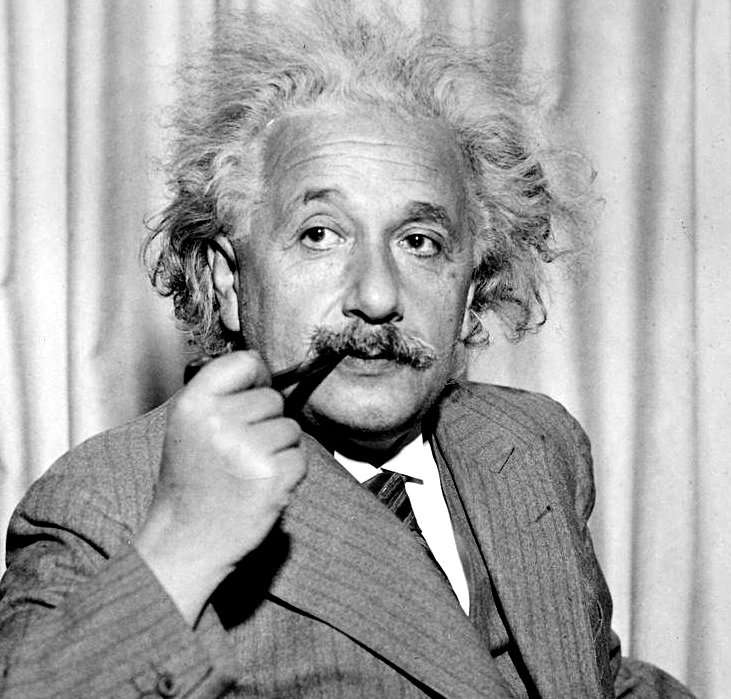
\includegraphics{AuthorIcon}

\latexprintindex

\end{document} 
